% 高一132_川沙中学_期中.tex
%   —— 高一上数学"2026-2027 年川沙中学高一上期中"（试卷版/答案版）
% 试卷版：xelatex 高一132_川沙中学_期中.tex
% 答案版：xelatex "\def\isanswer{1}% 高一132_川沙中学_期中.tex
%   —— 高一上数学"2026-2027 年川沙中学高一上期中"（试卷版/答案版）
% 试卷版：xelatex 高一132_川沙中学_期中.tex
% 答案版：xelatex "\def\isanswer{1}% 高一132_川沙中学_期中.tex
%   —— 高一上数学"2026-2027 年川沙中学高一上期中"（试卷版/答案版）
% 试卷版：xelatex 高一132_川沙中学_期中.tex
% 答案版：xelatex "\def\isanswer{1}% 高一132_川沙中学_期中.tex
%   —— 高一上数学"2026-2027 年川沙中学高一上期中"（试卷版/答案版）
% 试卷版：xelatex 高一132_川沙中学_期中.tex
% 答案版：xelatex "\def\isanswer{1}\input{高一132_川沙中学_期中.tex}"
% 紧凑版：xelatex "\def\iscompact{1}\input{高一132_川沙中学_期中.tex}"
%
% 原始材料：微信公众号"魔都数学加油站"文章，作者破晓，2026-11-14 19:00 发布；
% 连载"27学年高一132"，原文标题"27学年高一132——2026-2027年上海市川沙中学高一上期中"；
% 原文链接：https://mp.weixin.qq.com/s/VBG01CrUNMIYWWHhSfz8JQ。
% 正文为 11 张 PNG 页（01、04、06、07、09、11 为 2560x3620，02、03、05、08、10 为 4762x6735），
% 题目下印有【解析】，为讲评版。题目、解析均据原图转录；
% 卷面粉红色水印"魔都数学加油站"及公众号页脚未录入。全卷 2 幅插图：第 14 题四幅坐标图选项、
% 第 18 题矩形 OCPD 与小路 EF 示意图，均取原卷 04／07 页截图去水印。
%
% 卷首标题：原卷印作"2026-2027 年川沙中学高一上期中"（公众号标题中的"上海市"
% 卷面标题行没有，本稿照卷面），年份区间按全稿惯例排 en dash；原卷未印副标题，
% 本卷为期中卷、跨集合与常用逻辑用语／不等式／函数三章，按题目内容标为
% "集合与常用逻辑用语、不等式、函数"（与 125／126／128／129／131 同期中卷口径相同）：
% 集合与逻辑见 Q5、Q6、Q17、Q21，不等式见 Q3、Q4、Q9、Q10、Q12、Q13、Q15、Q16、Q19，
% 函数（幂函数、指数／对数、基本不等式应用）见 Q7、Q8、Q11、Q14、Q18、Q20。
%
% 题号体例：本卷共 19 题——一、填空题 3—12（10 题）、二、选择题 13—16（4 题）、
% 三、解答题 17—21（5 题）。三节分别 \setcounter{enumi}{2}／{12}／{16}。
%
% 与原卷的排版差异：
%   ① 原文从第 3 题起，本稿保留原题号（见上"题号体例"）；
%   ② 原卷每题下直接印【解析】，本稿按全稿惯例置于答案版；第 13 题答案 D 印在题干
%      括号内、无独立答案段，按 高一37／52／53／55／63／64／128／131 成例括号留空、
%      另提 \ans{$D$}；第 14—16 题答案在解析末句"故选 …"，括号内留空、不另提 \ans{}；
%   ③ 原卷未印副标题，本稿按"知识模块"口径补出；
%   ④ 原卷填空横线按全稿惯例排为 \blankline[4.4em]；选择题括号排 \mbox{（\quad）}、
%      选项段前按惯例加 \keepwithprev；解答题不留作答区（原卷为讲评版，与 109—131 同）；
%   ⑤ 原卷数集排斜体 $R^+$／$R$／$Z$／$N$，按全稿惯例改 \R^+／\R／\Z／\N；
%      绝对值排 \lvert…\rvert，集合描述竖线排 \mid；不等号按全稿惯例排 \leqslant／\geqslant；
%      补集照原卷上划线排 \overline{B}；
%   ⑥ 子题标号 (1)(2)(3) 原卷用半角括号，照录；第 14 题四幅坐标图选项按原卷 2×2 排布
%      合并裁为一张 \includegraphics（未用 TikZ 重绘，以保证与原卷一致），题前加
%      \needvspace{9cm} 守卫；第 18 题图取 07 页截图，题前按惯例加 \needvspace{7cm} 守卫
%      （照 高一120／127／129／131 成例），两者守卫都放在 \item 之前；
%   ⑦ 原卷 Q7 解析跨 01—02 页、Q10 解析跨 02—03 页、Q12 解析跨 03—04 页、
%      Q14 解析跨 04—05 页、Q16 解析在 06 页、Q18 解析跨 07—08 页、
%      Q20 解析跨 08—09 页、Q21 解析跨 10—11 页，本稿按题合并连续排版；
%      末页第 11 页为 Q21 (3) 解析的续尾，按实际印刷行单列。
%
% 判别式字形：第 10 题 $\triangle=4(a-1)^2+16(a-1)<0$、第 11 题
%   $\triangle=4(m-2)^2-4(m^2-3m+3)=-4m+4>0$ 两处原卷均排 $\triangle$（等边、扁），
%   逐处放大核对、字形一致，照录 \triangle；与 高一129／131 同题排 $\Delta$（等腰、高）不同。
%   全卷 \triangle 兼作第 18 题「$\triangle PCE\sim\triangle FDP$」「$\triangle OEF$」的几何
%   三角形记号，全卷未出现 \Delta。
%
% 子集符号：第 5 题解析 $B\subseteq A$、第 17 题 (2) 解析 $A\subseteq B$ 均印带下划线，
%   照录 \subseteq；全卷未出现单线 \subset。
%
% 原卷存疑照录：
%   第 9 题题干作"充分非必要条件"、解析作"充分不必要条件"，措辞不同，照录；
%   第 10 题解析"当 $a-1=0$ 时，$-4\geq0$，不等式不成立，$a=1$ 满足题意"照录；
%   第 11 题解析"所以 $2(m-1)+\dfrac1{m-1}\leq-2\sqrt2$"由上一行 $2(1-m)+\dfrac1{1-m}\geq2\sqrt2$
%     直接变号得到，照录；
%   第 12 题解析"由 $x\in Z$，$-7<-2\sqrt{10}<-6$"与"即 $k^2+7k+10\leq0$，解得 $-5\leq k\leq-2$"照录；
%   第 16 题解析"令 $52\times(930+a)=-52$，解得 $a=-931$"（按式应为 $a=-931$ 之外的解）照录；
%   第 19 题 (2) 解析"所以 $-2<a<1,-2<b<1$"数学式内半角逗号，照录；
%   第 20 题 (3) 解析"最小值为 $3-\dfrac12+\dfrac52-1+2-\dfrac32=\dfrac92$"与
%     "故 $M(2,6)=\dots$ 的最小值为 9"两处结论并列，照录；
%   第 21 题 (1) 解析"$0+2\in M,0+4\in M,4-2\in M,0\pm0=0\in M$"、
%     "$2+2=4\in M,2-2=0\in M,4-4=0\in M$"、(3) 各连写等式内半角逗号，照录；
%   第 21 题 (3) 解析"即 $a_1+a_2+a_3+\cdots+a_n=\dfrac n2 a_n$，"句末用半角逗号，照录。
%
% 行数复核：见文末"行数复核"注（逐题 \step 条数与原卷印刷行逐题相等，cases 块作一个印刷行计）。
%   第 13 题只印括号内答案、提 \ans{}，不计入 \step 账；第 14—16 题答案在解析末句，
%   括号内留空、不另提 \ans{}。
%
\documentclass[a4paper,11pt]{article}
\usepackage{common}

\begin{document}

\examtitlest[3]{2026--2027 年川沙中学高一上期中}{集合与常用逻辑用语、不等式、函数}

\bigsec{一、填空题}

\begin{enumerate}
\setcounter{enumi}{2}

\item 已知 $a$、$b\in\R^+$ 且 $ab=2$，则 $a+2b$ 的最小值为\blankline[4.4em].

\ifanswer
\solbegin
\step{因为 $a\in\R^+$，$b\in\R^+$ 且 $ab=2$，}
\step{由基本不等式得 $a+2b\geq2\sqrt{a\cdot2b}=2\sqrt{2ab}=2\sqrt4=4$.}
\step{等号当且仅当 $a=2b$ 时成立，结合 $ab=2$ 解得 $b=1$，$a=2$，}
\step{所以 $a+2b$ 的最小值为 $4$.}
\solend
\fi

\item 如果幂函数 $f(x)=(m^2-3m-3)x^{m^2+m-3}$ 在 $(0,+\infty)$ 上是增函数，则实数 $m=$\blankline[4.4em].

\ifanswer
\solbegin
\step{由已知得 $\begin{cases}m^2-3m-3=1\\m^2+m-3>0\end{cases}$，所以 $m=4$.}
\solend
\fi

\item 已知集合 $A=\{1,2\}$，集合 $B=\{x\mid ax=6\}$，若 $A\cup B=A$，则 $a$ 的所有取值构成的集合为\blankline[4.4em].

\ifanswer
\solbegin
\step{因为 $A\cup B=A$，所以 $B\subseteq A$，}
\step{当 $a=0$ 时，$B=\varnothing$，满足 $B\subseteq A$；}
\step{当 $a\ne0$ 时，$B=\left\{\dfrac6a\right\}$，则 $\dfrac6a=1$ 或 $\dfrac6a=2$，解得 $a=6$ 或 $a=3$，}
\step{综上所述，$a$ 的所有取值构成的集合为 $\{0,3,6\}$.}
\solend
\fi

\item 设全集为 $\R$，$A=\{y\mid y=-x^2+2x+1\}$，$B=\{x\mid y=\ln(x-1)\}$，则 $A\cap B=$\blankline[4.4em].

\ifanswer
\solbegin
\step{$A=\{y\mid y=-x^2+2x+1\}=\{y\mid y=-(x-1)^2+2\}=\{y\mid y\leq2\}$，}
\step{$B=\{x\mid y=\ln(x-1)\}=\{x\mid x>1\}$，则 $A\cap B=(1,2]$.}
\solend
\fi

\item 已知 $x\in\R$，则方程 $\lvert 6-x\rvert+\lvert 6x-3\rvert=\lvert 5x+3\rvert$ 的解集为\blankline[4.4em].

\ifanswer
\solbegin
\step{当 $x<-\dfrac35$ 时，$6-x>0$，$6x-3<0$，$5x+3<0$，}
\step{原方程为 $6-x-6x+3=-5x-3$，解得 $x=6$，不满足 $x<-\dfrac35$；}
\step{当 $-\dfrac35\leq x\leq\dfrac12$ 时，$5x+3\geq0$，$6x-3<0$，$6-x>0$，}
\step{原方程为 $6-x+3-6x=5x+3$，解得 $x=\dfrac12$；}
\step{当 $\dfrac12<x\leq6$ 时，$5x+3>0$，$6x-3>0$，$6-x\geq0$，}
\step{原方程为 $6-x+6x-3=5x+3$，即 $0=0$，恒成立，所以 $\dfrac12<x\leq6$；}
\step{当 $x>6$ 时，$5x+3\geq0$，$6x-3>0$，$6-x<0$，}
\step{原方程为 $x-6+6x-3=5x+3$，解得 $x=6$，不满足 $x>6$；}
\step{综上 $\dfrac12\leq x\leq6$，所以原方程的解集为 $\left\{x\mid\dfrac12\leq x\leq6\right\}$.}
\solend
\fi

\item 已知 $\log_2 3=a,2^b=7$，用 $a,b$ 表示 $\log_{42}56$ 为\blankline[4.4em].

\ifanswer
\solbegin
\step{$\log_{42}56=\dfrac{\log_2 56}{\log_2 42}=\dfrac{\log_2(7\times8)}{\log_2(6\times7)}=\dfrac{\log_2 7+\log_2 8}{\log_2 6+\log_2 7}$}
\step{$=\dfrac{\log_2 7+\log_2 2^3}{\log_2 2+\log_2 3+\log_2 7}=\dfrac{b+3}{1+a+b}$.}
\solend
\fi

\item 已知 $\dfrac13<x<\dfrac12$ 是不等式 $\lvert x-m\rvert<1$ 成立的充分非必要条件，则 $m$ 的取值范围是\blankline[4.4em].

\ifanswer
\solbegin
\step{因为 $\lvert x-m\rvert<1$，所以 $-1<x-m<1$，所以 $m-1<x<m+1$，}
\step{所以 $m-1<x<m+1$ 成立的充分不必要条件是 $\dfrac13<x<\dfrac12$，}
\step{所以 $\begin{cases}m-1\leq\dfrac13\\m+1\geq\dfrac12\end{cases}$，解得 $-\dfrac12\leq m\leq\dfrac43$，故 $m$ 的取值范围是 $\left[-\dfrac12,\dfrac43\right]$.}
\solend
\fi

\item 若关于 $x$ 的不等式 $(a-1)x^2+2(a-1)x-4\geq0$ 的解集为空集，则 $a$ 的取值范围是\blankline[4.4em].

\ifanswer
\solbegin
\step{关于 $x$ 的不等式 $(a-1)x^2+2(a-1)x-4\geq0$ 的解集为 $\varnothing$，}
\step{当 $a-1=0$ 时，$-4\geq0$，不等式不成立，$a=1$ 满足题意；}
\step{当 $a-1>0$ 时，$a>1$，不等式的解集不为空集，不满足题意；}
\step{当 $a-1<0$ 时，$a<1$，当 $\triangle=4(a-1)^2+16(a-1)<0$ 时，即 $(a-1)(a+3)<0$，}
\step{解得 $-3<a<1$，满足题意；}
\step{综上，实数 $a$ 的取值范围是 $\{a\mid-3<a\leq1\}$.}
\solend
\fi

\item 已知关于 $x$ 的方程 $x^2+2(m-2)x+m^2-3m+3=0$ 有两个不相等的实数根 $x_1$、$x_2$，则 $\dfrac{mx_1}{x_1-1}+\dfrac{mx_2}{x_2-1}-\dfrac{2}{x_1+x_2-2}$ 的最大值为\blankline[4.4em].

\ifanswer
\solbegin
\step{关于 $x$ 的方程 $x^2+2(m-2)x+m^2-3m+3=0$ 有两个不相等的实数根 $x_1$、$x_2$，}
\step{则 $\triangle=4(m-2)^2-4(m^2-3m+3)=-4m+4>0$，得 $m<1$，}
\step{且 $x_1+x_2=-2(m-2)$，$x_1x_2=m^2-3m+3$，}
\step{$\dfrac{mx_1}{x_1-1}+\dfrac{mx_2}{x_2-1}-\dfrac{2}{x_1+x_2-2}=\dfrac{m[2x_1x_2-(x_1+x_2)]}{x_1x_2-(x_1+x_2)+1}+\dfrac1{m-1}$}
\step{$=\dfrac{2m(m-1)^2}{m^2-m}+\dfrac1{m-1}=2(m-1)+\dfrac1{m-1}$，}
\step{又因为 $m<1$，所以 $m-1<0$，则 $1-m>0$，}
\step{所以 $2(1-m)+\dfrac1{1-m}\geq2\sqrt{2(1-m)\cdot\dfrac1{1-m}}=2\sqrt2$，}
\step{当且仅当 $2(1-m)=\dfrac1{1-m}$ 时，即 $m=1-\dfrac{\sqrt2}2$ 时取等号，}
\step{所以 $2(m-1)+\dfrac1{m-1}\leq-2\sqrt2$，即 $\dfrac{mx_1}{x_1-1}+\dfrac{mx_2}{x_2-1}-\dfrac2{x_1+x_2-2}$ 的最大值为 $-2\sqrt2$.}
\solend
\fi

\item 若使集合 $A=\{x\mid(kx-k^2-10)(x-1)>0,x\in\Z\}$ 中的元素个数最少，则实数 $k$ 的取值范围是\blankline[4.4em].

\ifanswer
\solbegin
\step{由题意集合 $A=\{x\mid(kx-k^2-10)(x-1)>0,\ x\in\Z\}$，}
\step{$k=0$ 时，不等式解得 $x<1$，有无数个整数解；}
\step{$k\ne0$ 时，则不等式变形为 $k\left(x-k-\dfrac{10}k\right)(x-1)>0$，}
\step{当 $k>0$ 时，$k+\dfrac{10}k\geq2\sqrt{10}$，仅当 $k=\sqrt{10}$ 时等号成立，}
\step{此时不等式解得 $x>k+\dfrac{10}k$ 或 $x<1$，有无数个整数解；}
\step{当 $k<0$ 时，$k+\dfrac{10}k=-\left[(-k)+\left(-\dfrac{10}k\right)\right]\leq-2\sqrt{10}$，仅当 $k=-\sqrt{10}$ 时等号成立，}
\step{此时不等式解得 $k+\dfrac{10}k<x<1$，}
\step{由 $x\in\Z$，$-7<-2\sqrt{10}<-6$，要使集合 $A$ 中的元素最少，则 $k+\dfrac{10}k\geq-7$，}
\step{即 $k^2+7k+10\leq0$，解得 $-5\leq k\leq-2$，故实数 $k$ 的取值范围是 $[-5,-2]$.}
\solend
\fi

\end{enumerate}

\bigsec{二、选择题}

\begin{enumerate}
\setcounter{enumi}{12}

\item 下列说法正确的是\mbox{（\quad）}

\keepwithprev
A. 若 $a>b$，则 $\dfrac1a<\dfrac1b$\qquad\qquad B. 若 $a>b$，$c>d$，则 $ac>bd$

C. 若 $a>b$，则 $ac^2>bc^2$\qquad\qquad D. 若 $ac^2>bc^2$，则 $a>b$

\ifanswer
\ans{$D$}
\fi

% 第 14 题四幅坐标图选项是一整块，守卫放在 \item 之前
\needvspace{9cm}
\item 在同一坐标系内，函数 $y=x^a(a\ne0)$ 和 $y=ax-\dfrac1a$ 的图象可能是\mbox{（\quad）}

\keepwithprev
\begin{center}
% 四幅坐标图选项取原卷 04 页截图去粉色水印，按原卷 2×2 排布合并为一张
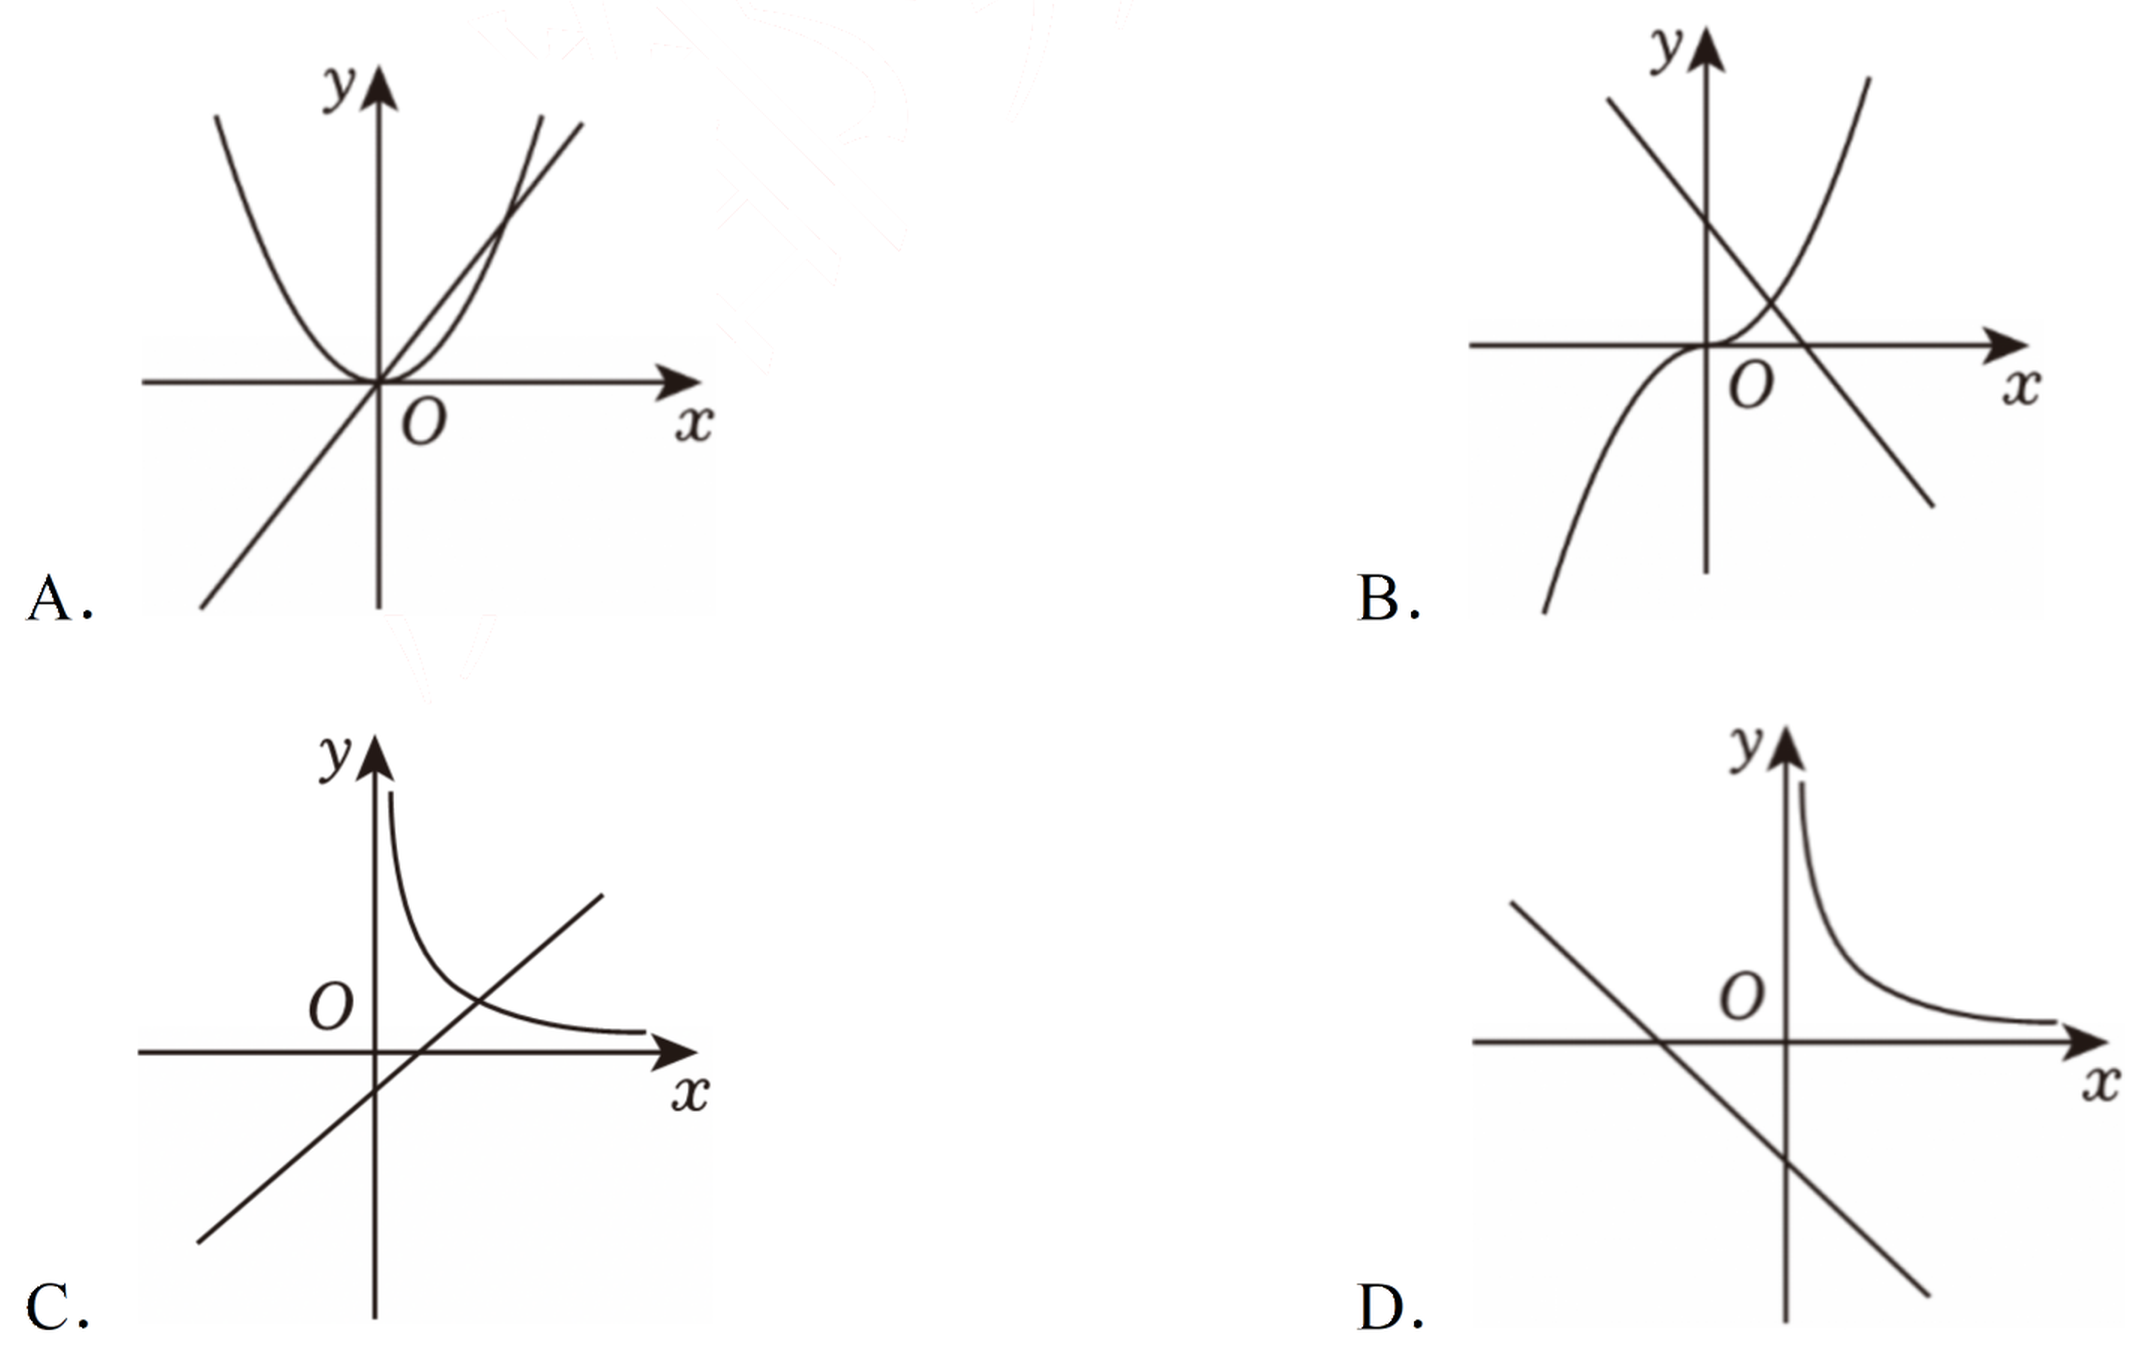
\includegraphics[width=0.80\textwidth]{figures/gao132_q14.png}
\end{center}

\ifanswer
\solbegin
\step{当 $a>0$ 时，$y=ax-\dfrac1a$ 严格增，当 $a<0$ 时，$y=ax-\dfrac1a$ 严格减，}
\step{对于 $A$，因为 $a\ne0$，所以直线 $y=ax-\dfrac1a$ 不过原点，故 $A$ 错误；}
\step{对于 $B$，由函数 $y=x^a(a\ne0)$ 的图象得 $a>1$，}
\step{由 $y=ax-\dfrac1a$ 的图象得 $a<0$，互相矛盾，故 $B$ 错误；}
\step{对于 $C$，由函数 $y=x^a(a\ne0)$ 的图象得 $a>1$，}
\step{由 $y=ax-\dfrac1a$ 的图象得 $a>0$ 且 $-\dfrac1a<0$，符合题意，故 $C$ 正确；}
\step{对于 $D$，由函数 $y=x^a(a\ne0)$ 的图象得 $a<0$，}
\step{由 $y=ax-\dfrac1a$ 的图象得 $a<0$ 且 $-\dfrac1a<0$，互相矛盾，故 $D$ 错误；}
\step{故选 $C$.}
\solend
\fi

\item 中国的 $5G$ 技术领先世界，在 $5G$ 技术中，最大数据传输速率 $C$ 取决于信道带宽 $W$，$C$ 与 $W$ 满足 $C=W\log_2\left(1+\dfrac SN\right)$，其中 $\dfrac SN$ 称为信噪比（单位：$dB$）. 若不改变带宽 $W$，初始信噪比 $\dfrac SN$ 为 $1000$，那么为了使 $C$ 增加 $30\%$，需要将信噪比 $\dfrac SN$ 从 $1000$ 提升至大约\mbox{（\quad）}

\keepwithprev
A. $5000$\qquad\qquad B. $6000$\qquad\qquad C. $7000$\qquad\qquad D. $8000$

\ifanswer
\solbegin
\step{由题意得 $\dfrac SN=1000$ 时，$C=W\log_2(1+1000)\approx W\log_2 1000$，}
\step{要使 $C$ 增加 $30\%$，则 $(1+30\%)C=W\log_2\left(1+\dfrac SN\right)$，即 $1.3C\approx W\log_2\dfrac SN$，}
\step{所以 $1.3\approx\log_{1000}\dfrac SN=\dfrac{\lg\frac SN}{\lg1000}$，所以 $\lg\dfrac SN=3.9$，所以 $\dfrac SN=10^{3.9}\approx8000$.}
\step{故选 $D$.}
\solend
\fi

\item 对于 $a\in\R$，设非空集合 $A=\left\{x\mid\dfrac{(x^2-930x+a)(x-52)}{x+a}=0\right\}$，记 $A$ 中的所有元素之和为 $S(a)$，所有元素之积为 $T(a)$，则下列说法中，不正确的是\mbox{（\quad）}

\keepwithprev
A. 存在实数 $a$，使得 $S(a)=930$

B. 存在实数 $a$，使得 $T(a)=517$

C. 不存在实数 $a$，使得 $T(a)=0$

D. 恰存在 $1$ 个实数 $a$，使得 $T(a)=-52$

\ifanswer
\solbegin
\step{由分式值为 $0$，得分子为 $0$ 且分母不为 $0$，}
\step{分子 $(x^2-930x+a)(x-52)=0$ 的根为 $x=52$}
\step{及方程 $x^2-930x+a=0$ 的两根 $x_1$，$x_2$，}
\step{由根与系数的关系得 $x_1+x_2=930$，$x_1\cdot x_2=a$，}
\step{分母限制 $x\ne-a$，需要剔除等于 $-a$ 的根，}
\step{选项 $A$，取 $a=-52$，$x=52$ 为增根舍去，集合 $A=\{x_1,x_2\}$，}
\step{元素之和 $S(a)=930$，故 $A$ 正确；}
\step{选项 $B$，当无增根时，$T(a)=52a$，令 $52a=517$，得 $a=\dfrac{517}{52}$，}
\step{验证无增根，存在这样的 $a$，故 $B$ 正确；}
\step{选项 $C$，若 $T(a)=0$，则 $0\in A$，代入分子得 $a=0$，}
\step{但 $a=0$ 时分母 $x\ne0$，$x=0$ 为增根，$0$ 不能属于集合 $A$，}
\step{故不存在 $a$ 使得 $T(a)=0$，故 $C$ 正确；}
\step{选项 $D$，当无增根时，令 $52a=-52$，得 $a=-1$；}
\step{当 $x=-a$ 是二次方程的根且不等于 $52$ 时，}
\step{令 $52\times(930+a)=-52$，解得 $a=-931$，验证符合条件；}
\step{当 $a=-52$ 时，$x=52$，舍去，}
\step{集合 $A=\{x_1,x_2\}$，$T(a)=a=-52$，得到两个满足条件的 $a$；}
\step{因此存在 $3$ 个满足条件的 $a$，故 $D$ 错误.}
\step{故选 $D$.}
\solend
\fi

\end{enumerate}

\bigsec{三、解答题}

\begin{enumerate}
\setcounter{enumi}{16}

\item 已知全集 $U=\R$，集合 $A=\left\{x\mid\dfrac{x}{x-3}<0\right\}$，$B=\{x\mid(x-a)(x+4-a)<0\}$.

(1) 当 $a=2$ 时，求 $\overline{B}$、$A\cap\overline{B}$；

(2) 若 $A\cap B=A$，求实数 $a$ 的取值范围.

\ifanswer
\solbegin
\step{(1) $\dfrac{x}{x-3}<0$，即 $x(x-3)<0$，解得 $A=\{x\mid0<x<3\}$，}
\step{当 $a=2$ 时，$B=\{x\mid(x-a)(x+4-a)<0\}=\{x\mid-2<x<2\}$，}
\step{则 $\overline{B}=\{x\mid x\leq-2$ 或 $x\geq2\}$，故 $A\cap\overline{B}=\{x\mid2\leq x<3\}$；}
\step{(2) $A\cap B=A$，则 $A\subseteq B$，故 $\begin{cases}a-4\leq0\\a\geq3\end{cases}$，解得 $3\leq a\leq4$，}
\step{故实数 $a$ 的取值范围是 $\{a\mid3\leq a\leq4\}$.}
\solend
\fi

% 第 18 题是"题干 + 图"约 7cm 的一整块，守卫放在 \item 之前
\needvspace{7cm}
\item 如图，$OA$、$OB$ 是两条长度足够长的互相垂直的笔直小路，矩形 $OCPD$ 的顶点 $C$、$D$ 分别在 $OA$、$OB$ 上，且该矩形区域内种满了荷花. 为了让观赏者有更好的观赏体验，现计划经过点 $P$ 修一条小路 $EF$，其中点 $E$ 在小路 $OA$ 上，点 $F$ 在小路 $OB$ 上，并在 $\triangle OEF$ 区域内种满荷花. 已知 $OD=25m$，$OC=40m$，且小路 $EF$ 要完全位于一个以 $O$ 为顶点的，边长为 $100$ m 的正方形内部（包括边界）. 记 $\triangle OEF$ 的面积为 $S$m$^2$.

(1) 设 $EC=x\cdot m$，试用 $x$ 表示 $OF$，并求 $x$ 的取值范围.

(2) 当 $EC$ 的长度为多少时，$S$ 取得最小值？最小值是多少？

\begin{center}
% 图取原卷 07 页截图去粉色水印，3× LANCZOS 放大
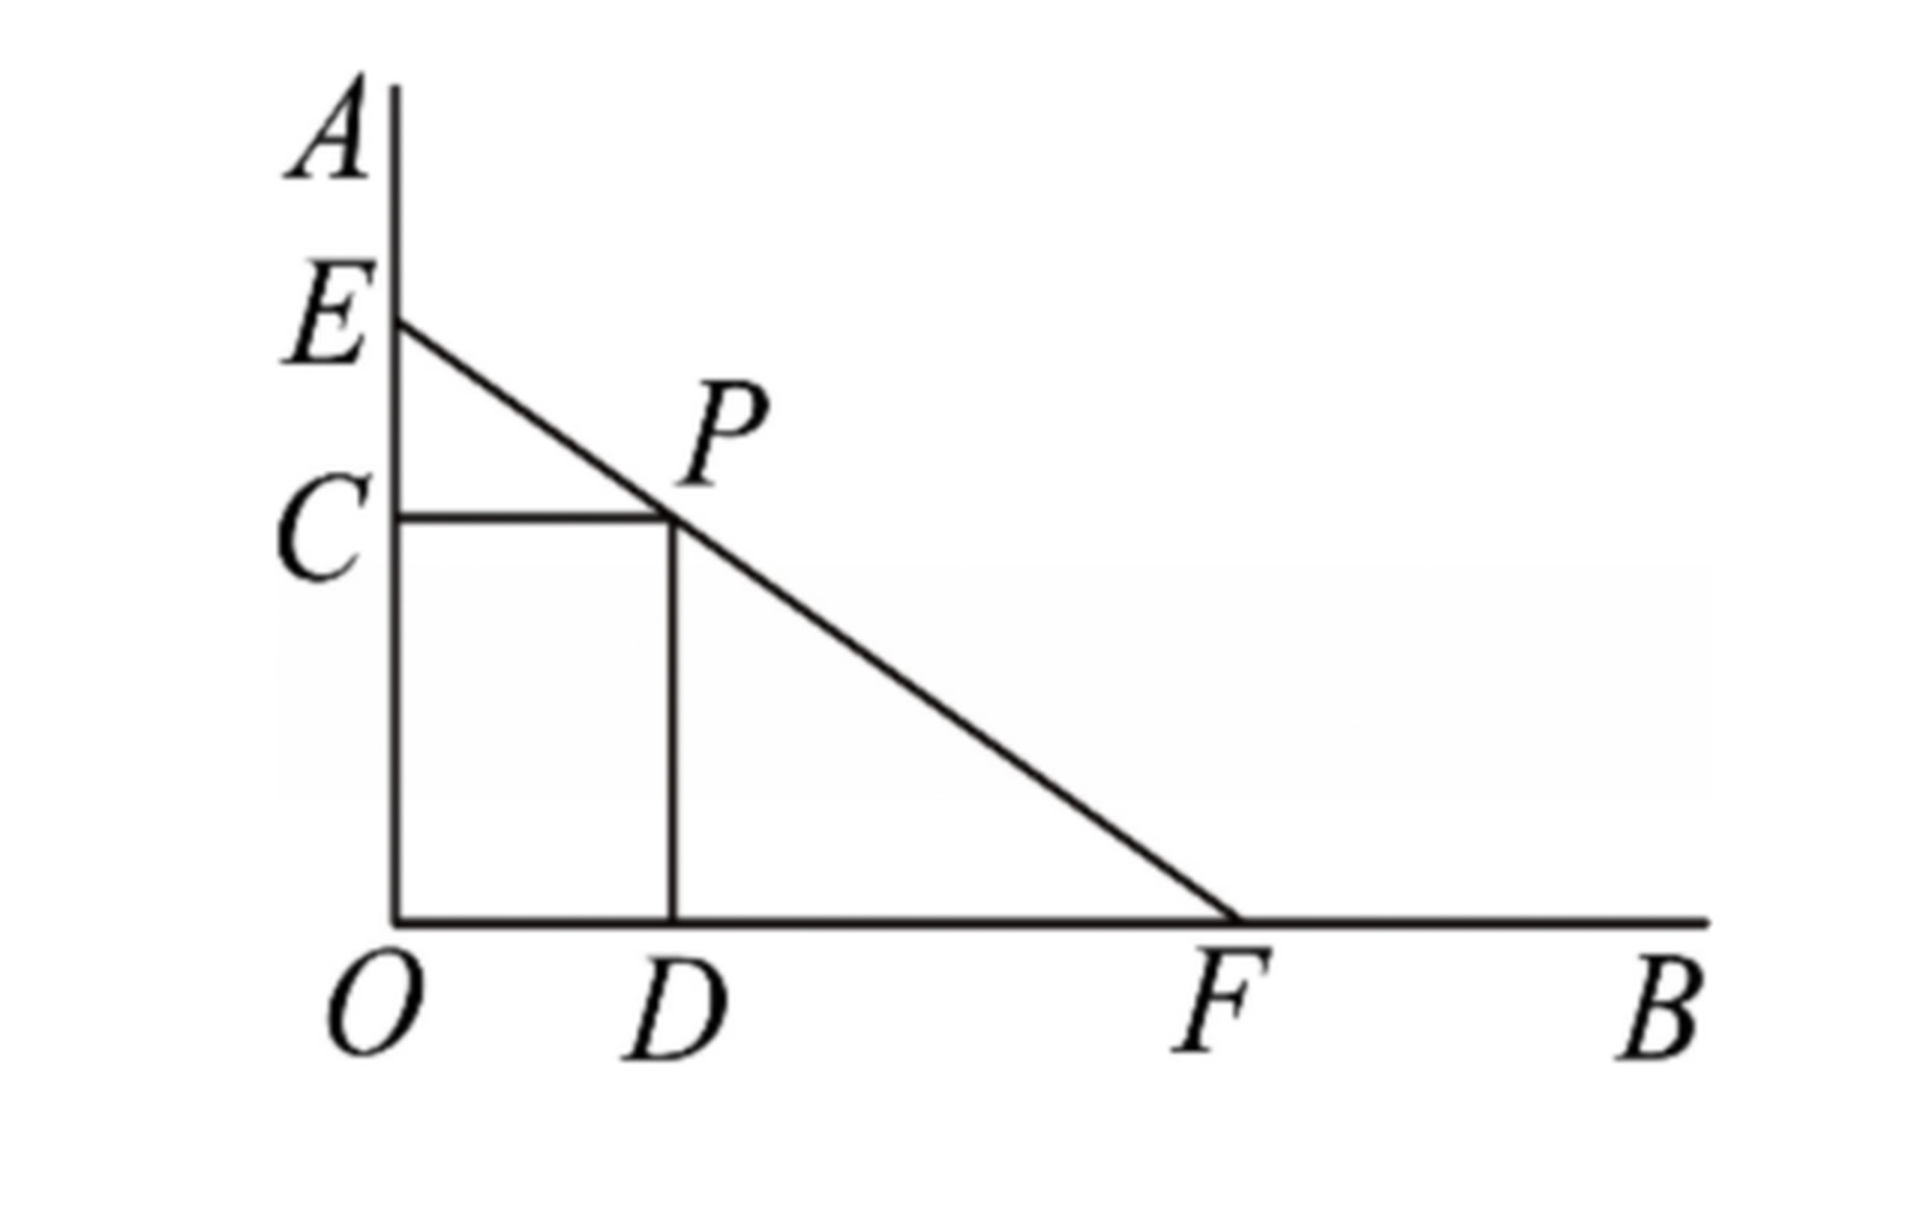
\includegraphics[width=0.32\textwidth]{figures/gao132_q18.png}
\end{center}

\ifanswer
\solbegin
\step{(1) 由题意得 $x\leq60$，}
\step{$\triangle PCE\sim\triangle FDP$，所以 $\dfrac{EC}{CP}=\dfrac{PD}{DF}$，即 $\dfrac{x}{25}=\dfrac{40}{DF}$，得 $DF=\dfrac{1000}{x}$m，}
\step{所以 $OF=OD+DF=\left(25+\dfrac{1000}x\right)$m，}
\step{所以 $25+\dfrac{1000}x\leq100$，解得 $x\geq\dfrac{40}3$；}
\step{综上，$\dfrac{40}3\leq x\leq60$；}
\step{(2) 由 $OE=OC+CE=(40+x)$m，}
\step{所以 $S=\dfrac12 OF\cdot OE=\dfrac12\left(25+\dfrac{1000}x\right)(40+x)$}
\step{$=\dfrac12\left(1000+25x+\dfrac{40000}x+1000\right)$m$^2$，}
\step{由基本不等式得 $S\geq\dfrac12\left(2000+2\sqrt{25x\cdot\dfrac{40000}x}\right)=2000$m$^2$，}
\step{当且仅当 $25x=\dfrac{40000}x$，即 $x=40$ 时取等号，}
\step{故 $EC=40$m 时，$S$ 取得最小值，为 $2000$m$^2$.}
\solend
\fi

\item 已知 $a>0$，$b>0$，请选择适当的方法证明.

(1) 若 $a\ne b$，证明：$a^3+b^3>a^2b+ab^2$；

(2) 若 $ab=1$，证明：$a^2+a<2$ 与 $b^2+b<2$ 不能同时成立.

\ifanswer
\solbegin
\step{(1) 因为 $a>0$，$b>0$，$a\ne b$，}
\step{所以 $a^3+b^3-a^2b-ab^2=a^2(a-b)+b^2(b-a)$}
\step{$=(a^2-b^2)(a-b)=(a-b)^2(a+b)>0$，所以 $a^3+b^3>a^2b+ab^2$.}
\step{(2) 假设 $a^2+a<2$ 与 $b^2+b<2$ 同时成立，所以 $-2<a<1,-2<b<1$，}
\step{又因为 $a>0,b>0$，所以 $0<a<1,0<b<1$，}
\step{所以 $0<ab<1$，这与 $ab=1$ 矛盾，}
\step{故 $a^2+a<2$ 与 $b^2+b<2$ 不可能同时成立.}
\solend
\fi

\item 若设 $M(a,n)=\lvert ax-1\rvert+\lvert ax-2\rvert+\cdots+\lvert ax-n\rvert$ 为曼哈顿扩张距离，它由 $n$ 个绝对值之和组成，其中 $n$ 为正整数.

(1) 若 $M(2,1)\leq5$，求 $x$ 的取值范围；

(2) 若 $k\leq M(2,2)$ 对一切实数 $x$ 恒成立，求实数 $k$ 的取值范围；

(3) $M(2,6)$ 是否存在最小值？若存在，求出该最小值与此时实数 $x$ 的取值范围；若不存在，说明理由.

\ifanswer
\solbegin
\step{(1) $M(2,1)=\lvert2x-1\rvert\leq5$，则不等式可化为 $-5\leq2x-1\leq5$，解得 $-2\leq x\leq3$，}
\step{所以 $x$ 的取值范围为 $[-2,3]$.}
\step{(2) 因为 $k\leq M(2,2)=\lvert2x-1\rvert+\lvert2x-2\rvert$ 对一切实数 $x$ 恒成立，}
\step{又 $\lvert2x-1\rvert+\lvert2x-2\rvert\geq\lvert(2x-1)-(2x-2)\rvert=1$，}
\step{当且仅当 $(2x-1)(2x-2)\leq0$，即 $\dfrac12\leq x\leq1$ 时取等号，}
\step{故 $k\leq1$，所以实数 $k$ 的取值范围为 $(-\infty,1]$.}
\step{(3) $M(2,6)=\lvert2x-1\rvert+\lvert2x-2\rvert+\lvert2x-3\rvert+\lvert2x-4\rvert+\lvert2x-5\rvert+\lvert2x-6\rvert$}
\step{$=2\left(\left\lvert x-\dfrac12\right\rvert+\lvert x-1\rvert+\left\lvert x-\dfrac32\right\rvert+\lvert x-2\rvert+\left\lvert x-\dfrac52\right\rvert+\lvert x-3\rvert\right)$，}
\step{其中 $\left\lvert x-\dfrac12\right\rvert+\lvert x-1\rvert+\left\lvert x-\dfrac32\right\rvert+\lvert x-2\rvert+\left\lvert x-\dfrac52\right\rvert+\lvert x-3\rvert$ 的几何意义为}
\step{在数轴上一点 $x$ 到 $\dfrac12,1,\dfrac32,2,\dfrac52,3$ 的距离之和，}
\step{要想距离之和最小，其中 $x\in\left[\dfrac12,3\right]$ 时，$\left\lvert x-\dfrac12\right\rvert+\lvert x-3\rvert$ 取得最小值，}
\step{当 $x\in\left[1,\dfrac52\right]$ 时，$\lvert x-1\rvert+\left\lvert x-\dfrac52\right\rvert$ 取得最小值，}
\step{当 $x\in\left[\dfrac32,2\right]$ 时，$\left\lvert x-\dfrac32\right\rvert+\lvert x-2\rvert$ 取得最小值，}
\step{综上，当 $x\in\left[\dfrac32,2\right]$ 时，$\left\lvert x-\dfrac12\right\rvert+\lvert x-1\rvert+\left\lvert x-\dfrac32\right\rvert+\lvert x-2\rvert+\left\lvert x-\dfrac52\right\rvert+\lvert x-3\rvert$}
\step{取得最小值，最小值为 $3-\dfrac12+\dfrac52-1+2-\dfrac32=\dfrac92$，}
\step{故 $M(2,6)=2\left(\left\lvert x-\dfrac12\right\rvert+\lvert x-1\rvert+\left\lvert x-\dfrac32\right\rvert+\lvert x-2\rvert+\left\lvert x-\dfrac52\right\rvert+\lvert x-3\rvert\right)$ 的}
\step{最小值为 $9$.}
\solend
\fi

\item 已知集合 $A=\{a_1,a_2,\cdots,a_n\}(0\leq a_1<a_2<\cdots<a_n,n\in\N,n\geq3)$ 具有性质 $Q$：对任意 $i,j(1\leq i\leq j\leq n)$，$a_i+a_j$ 与 $a_j-a_i$ 至少有一个属于集合 $A$；

(1) 判断集合 $M=\{0,2,4\}$ 与 $N=\{2,3,4\}$ 是否具有性质 $Q$，并说明理由；

(2) 已知 $A=\{a_1,a_2,a_3\}$ 具有性质 $Q$，当 $a_2=2026$ 时，求集合 $A$；

(3) 已知 $B=\{b_1,b_2,\cdots,b_{2026}\}$ 具有性质 $Q$，求 $\dfrac{b_1+b_2+\cdots+b_{2026}}{b_{2026}}$ 的值；

\ifanswer
\solbegin
\step{(1) 集合 $M=\{0,2,4\}$ 中，}
\step{因为 $0+2\in M,0+4\in M,4-2\in M,0\pm0=0\in M$，}
\step{$2+2=4\in M,2-2=0\in M,4-4=0\in M$，所以集合 $M$ 具有性质 $Q$；}
\step{集合 $N=\{2,3,4\}$ 中，因为 $3+3=6\notin N,3-3=0\notin N$，}
\step{所以集合 $N$ 不具有性质 $Q$.}
\step{(2) 因为 $a_1<a_2<a_3$，且 $A=\{a_1,a_2,a_3\}$ 具有性质 $Q$，}
\step{所以 $a_3+a_3\notin A,a_3-a_3=0\in A$，则 $a_1=0$，}
\step{又因为 $a_2+a_3>a_3$，所以 $a_2+a_3\notin A$，则 $a_3-a_2\in A$，}
\step{由集合的互异性得 $a_3-a_2=a_2$，而 $a_2=2026$，所以 $a_3=4052$，}
\step{故 $A=\{0,2026,4052\}$；}
\step{(3) 先证明一般结论：$A=\{a_1,a_2,\cdots,a_n\}(0\leq a_1<a_2<\cdots<a_n,n\in\N,n\geq3)$}
\step{具有性质 $Q$，则 $a_1+a_2+a_3+\cdots+a_n=\dfrac n2 a_n$.}
\step{因为 $A=\{a_1,a_2,\cdots,a_n\}(0\leq a_1<a_2<\cdots<a_n,n\in\N,n\geq3)$ 具有性质 $Q$，}
\step{所以 $a_n+a_n\notin A$，则 $a_n-a_n=0\in A$，则 $a_1=0$.}
\step{又因为 $0\leq a_1<a_2<\cdots<a_n$，所以 $0\leq a_n-a_n<a_n-a_{n-1}<\cdots<a_n-a_1$，}
\step{又因为 $a_n+a_{n-i}>a_n(i=1,2,\cdots,n-1)$，所以 $a_n+a_{n-i}\notin A$，}
\step{则 $a_n-a_{n-i}\in A$，}
\step{所以 $a_1=a_n-a_n,a_2=a_n-a_{n-1},a_3=a_n-a_{n-2},\cdots,a_n=a_n-a_1$.}
\step{所以 $a_1+a_2+a_3+\cdots+a_n$}
\step{$=(a_n-a_n)+(a_n-a_{n-1})+(a_n-a_{n-2})+\cdots+(a_n-a_1)$，}
\step{即 $a_1+a_2+a_3+\cdots+a_n=\dfrac n2 a_n$，}
\step{所以 $B=\{b_1,b_2,\cdots,b_{2026}\}$ 具有性质 $Q$，则 $b_1+b_2+\cdots+b_{2026}=\dfrac{2026}{2}b_{2026}$，}
\step{所以 $\dfrac{b_1+b_2+\cdots+b_{2026}}{b_{2026}}=\dfrac{2026}{2}=1013$.}
\solend
\fi

\end{enumerate}

% 行数复核：逐题数 \step 条数，合计 144 条（Q3：4；Q4：1；Q5：4；Q6：2；Q7：9；Q8：2；
% Q9：3；Q10：6；Q11：9；Q12：9；Q13：0；Q14：9；Q15：4；Q16：19；Q17：5；Q18：11；
% Q19：7；Q20：17；Q21：23），与原卷印刷行逐题相等（cases 块作一个印刷行计）。
% 第 13 题只印括号内答案、提 \ans{}，不计入 \step 账；第 14—16 题答案在解析末句，
% 括号内留空、不另提 \ans{}。

\end{document}
"
% 紧凑版：xelatex "\def\iscompact{1}% 高一132_川沙中学_期中.tex
%   —— 高一上数学"2026-2027 年川沙中学高一上期中"（试卷版/答案版）
% 试卷版：xelatex 高一132_川沙中学_期中.tex
% 答案版：xelatex "\def\isanswer{1}\input{高一132_川沙中学_期中.tex}"
% 紧凑版：xelatex "\def\iscompact{1}\input{高一132_川沙中学_期中.tex}"
%
% 原始材料：微信公众号"魔都数学加油站"文章，作者破晓，2026-11-14 19:00 发布；
% 连载"27学年高一132"，原文标题"27学年高一132——2026-2027年上海市川沙中学高一上期中"；
% 原文链接：https://mp.weixin.qq.com/s/VBG01CrUNMIYWWHhSfz8JQ。
% 正文为 11 张 PNG 页（01、04、06、07、09、11 为 2560x3620，02、03、05、08、10 为 4762x6735），
% 题目下印有【解析】，为讲评版。题目、解析均据原图转录；
% 卷面粉红色水印"魔都数学加油站"及公众号页脚未录入。全卷 2 幅插图：第 14 题四幅坐标图选项、
% 第 18 题矩形 OCPD 与小路 EF 示意图，均取原卷 04／07 页截图去水印。
%
% 卷首标题：原卷印作"2026-2027 年川沙中学高一上期中"（公众号标题中的"上海市"
% 卷面标题行没有，本稿照卷面），年份区间按全稿惯例排 en dash；原卷未印副标题，
% 本卷为期中卷、跨集合与常用逻辑用语／不等式／函数三章，按题目内容标为
% "集合与常用逻辑用语、不等式、函数"（与 125／126／128／129／131 同期中卷口径相同）：
% 集合与逻辑见 Q5、Q6、Q17、Q21，不等式见 Q3、Q4、Q9、Q10、Q12、Q13、Q15、Q16、Q19，
% 函数（幂函数、指数／对数、基本不等式应用）见 Q7、Q8、Q11、Q14、Q18、Q20。
%
% 题号体例：本卷共 19 题——一、填空题 3—12（10 题）、二、选择题 13—16（4 题）、
% 三、解答题 17—21（5 题）。三节分别 \setcounter{enumi}{2}／{12}／{16}。
%
% 与原卷的排版差异：
%   ① 原文从第 3 题起，本稿保留原题号（见上"题号体例"）；
%   ② 原卷每题下直接印【解析】，本稿按全稿惯例置于答案版；第 13 题答案 D 印在题干
%      括号内、无独立答案段，按 高一37／52／53／55／63／64／128／131 成例括号留空、
%      另提 \ans{$D$}；第 14—16 题答案在解析末句"故选 …"，括号内留空、不另提 \ans{}；
%   ③ 原卷未印副标题，本稿按"知识模块"口径补出；
%   ④ 原卷填空横线按全稿惯例排为 \blankline[4.4em]；选择题括号排 \mbox{（\quad）}、
%      选项段前按惯例加 \keepwithprev；解答题不留作答区（原卷为讲评版，与 109—131 同）；
%   ⑤ 原卷数集排斜体 $R^+$／$R$／$Z$／$N$，按全稿惯例改 \R^+／\R／\Z／\N；
%      绝对值排 \lvert…\rvert，集合描述竖线排 \mid；不等号按全稿惯例排 \leqslant／\geqslant；
%      补集照原卷上划线排 \overline{B}；
%   ⑥ 子题标号 (1)(2)(3) 原卷用半角括号，照录；第 14 题四幅坐标图选项按原卷 2×2 排布
%      合并裁为一张 \includegraphics（未用 TikZ 重绘，以保证与原卷一致），题前加
%      \needvspace{9cm} 守卫；第 18 题图取 07 页截图，题前按惯例加 \needvspace{7cm} 守卫
%      （照 高一120／127／129／131 成例），两者守卫都放在 \item 之前；
%   ⑦ 原卷 Q7 解析跨 01—02 页、Q10 解析跨 02—03 页、Q12 解析跨 03—04 页、
%      Q14 解析跨 04—05 页、Q16 解析在 06 页、Q18 解析跨 07—08 页、
%      Q20 解析跨 08—09 页、Q21 解析跨 10—11 页，本稿按题合并连续排版；
%      末页第 11 页为 Q21 (3) 解析的续尾，按实际印刷行单列。
%
% 判别式字形：第 10 题 $\triangle=4(a-1)^2+16(a-1)<0$、第 11 题
%   $\triangle=4(m-2)^2-4(m^2-3m+3)=-4m+4>0$ 两处原卷均排 $\triangle$（等边、扁），
%   逐处放大核对、字形一致，照录 \triangle；与 高一129／131 同题排 $\Delta$（等腰、高）不同。
%   全卷 \triangle 兼作第 18 题「$\triangle PCE\sim\triangle FDP$」「$\triangle OEF$」的几何
%   三角形记号，全卷未出现 \Delta。
%
% 子集符号：第 5 题解析 $B\subseteq A$、第 17 题 (2) 解析 $A\subseteq B$ 均印带下划线，
%   照录 \subseteq；全卷未出现单线 \subset。
%
% 原卷存疑照录：
%   第 9 题题干作"充分非必要条件"、解析作"充分不必要条件"，措辞不同，照录；
%   第 10 题解析"当 $a-1=0$ 时，$-4\geq0$，不等式不成立，$a=1$ 满足题意"照录；
%   第 11 题解析"所以 $2(m-1)+\dfrac1{m-1}\leq-2\sqrt2$"由上一行 $2(1-m)+\dfrac1{1-m}\geq2\sqrt2$
%     直接变号得到，照录；
%   第 12 题解析"由 $x\in Z$，$-7<-2\sqrt{10}<-6$"与"即 $k^2+7k+10\leq0$，解得 $-5\leq k\leq-2$"照录；
%   第 16 题解析"令 $52\times(930+a)=-52$，解得 $a=-931$"（按式应为 $a=-931$ 之外的解）照录；
%   第 19 题 (2) 解析"所以 $-2<a<1,-2<b<1$"数学式内半角逗号，照录；
%   第 20 题 (3) 解析"最小值为 $3-\dfrac12+\dfrac52-1+2-\dfrac32=\dfrac92$"与
%     "故 $M(2,6)=\dots$ 的最小值为 9"两处结论并列，照录；
%   第 21 题 (1) 解析"$0+2\in M,0+4\in M,4-2\in M,0\pm0=0\in M$"、
%     "$2+2=4\in M,2-2=0\in M,4-4=0\in M$"、(3) 各连写等式内半角逗号，照录；
%   第 21 题 (3) 解析"即 $a_1+a_2+a_3+\cdots+a_n=\dfrac n2 a_n$，"句末用半角逗号，照录。
%
% 行数复核：见文末"行数复核"注（逐题 \step 条数与原卷印刷行逐题相等，cases 块作一个印刷行计）。
%   第 13 题只印括号内答案、提 \ans{}，不计入 \step 账；第 14—16 题答案在解析末句，
%   括号内留空、不另提 \ans{}。
%
\documentclass[a4paper,11pt]{article}
\usepackage{common}

\begin{document}

\examtitlest[3]{2026--2027 年川沙中学高一上期中}{集合与常用逻辑用语、不等式、函数}

\bigsec{一、填空题}

\begin{enumerate}
\setcounter{enumi}{2}

\item 已知 $a$、$b\in\R^+$ 且 $ab=2$，则 $a+2b$ 的最小值为\blankline[4.4em].

\ifanswer
\solbegin
\step{因为 $a\in\R^+$，$b\in\R^+$ 且 $ab=2$，}
\step{由基本不等式得 $a+2b\geq2\sqrt{a\cdot2b}=2\sqrt{2ab}=2\sqrt4=4$.}
\step{等号当且仅当 $a=2b$ 时成立，结合 $ab=2$ 解得 $b=1$，$a=2$，}
\step{所以 $a+2b$ 的最小值为 $4$.}
\solend
\fi

\item 如果幂函数 $f(x)=(m^2-3m-3)x^{m^2+m-3}$ 在 $(0,+\infty)$ 上是增函数，则实数 $m=$\blankline[4.4em].

\ifanswer
\solbegin
\step{由已知得 $\begin{cases}m^2-3m-3=1\\m^2+m-3>0\end{cases}$，所以 $m=4$.}
\solend
\fi

\item 已知集合 $A=\{1,2\}$，集合 $B=\{x\mid ax=6\}$，若 $A\cup B=A$，则 $a$ 的所有取值构成的集合为\blankline[4.4em].

\ifanswer
\solbegin
\step{因为 $A\cup B=A$，所以 $B\subseteq A$，}
\step{当 $a=0$ 时，$B=\varnothing$，满足 $B\subseteq A$；}
\step{当 $a\ne0$ 时，$B=\left\{\dfrac6a\right\}$，则 $\dfrac6a=1$ 或 $\dfrac6a=2$，解得 $a=6$ 或 $a=3$，}
\step{综上所述，$a$ 的所有取值构成的集合为 $\{0,3,6\}$.}
\solend
\fi

\item 设全集为 $\R$，$A=\{y\mid y=-x^2+2x+1\}$，$B=\{x\mid y=\ln(x-1)\}$，则 $A\cap B=$\blankline[4.4em].

\ifanswer
\solbegin
\step{$A=\{y\mid y=-x^2+2x+1\}=\{y\mid y=-(x-1)^2+2\}=\{y\mid y\leq2\}$，}
\step{$B=\{x\mid y=\ln(x-1)\}=\{x\mid x>1\}$，则 $A\cap B=(1,2]$.}
\solend
\fi

\item 已知 $x\in\R$，则方程 $\lvert 6-x\rvert+\lvert 6x-3\rvert=\lvert 5x+3\rvert$ 的解集为\blankline[4.4em].

\ifanswer
\solbegin
\step{当 $x<-\dfrac35$ 时，$6-x>0$，$6x-3<0$，$5x+3<0$，}
\step{原方程为 $6-x-6x+3=-5x-3$，解得 $x=6$，不满足 $x<-\dfrac35$；}
\step{当 $-\dfrac35\leq x\leq\dfrac12$ 时，$5x+3\geq0$，$6x-3<0$，$6-x>0$，}
\step{原方程为 $6-x+3-6x=5x+3$，解得 $x=\dfrac12$；}
\step{当 $\dfrac12<x\leq6$ 时，$5x+3>0$，$6x-3>0$，$6-x\geq0$，}
\step{原方程为 $6-x+6x-3=5x+3$，即 $0=0$，恒成立，所以 $\dfrac12<x\leq6$；}
\step{当 $x>6$ 时，$5x+3\geq0$，$6x-3>0$，$6-x<0$，}
\step{原方程为 $x-6+6x-3=5x+3$，解得 $x=6$，不满足 $x>6$；}
\step{综上 $\dfrac12\leq x\leq6$，所以原方程的解集为 $\left\{x\mid\dfrac12\leq x\leq6\right\}$.}
\solend
\fi

\item 已知 $\log_2 3=a,2^b=7$，用 $a,b$ 表示 $\log_{42}56$ 为\blankline[4.4em].

\ifanswer
\solbegin
\step{$\log_{42}56=\dfrac{\log_2 56}{\log_2 42}=\dfrac{\log_2(7\times8)}{\log_2(6\times7)}=\dfrac{\log_2 7+\log_2 8}{\log_2 6+\log_2 7}$}
\step{$=\dfrac{\log_2 7+\log_2 2^3}{\log_2 2+\log_2 3+\log_2 7}=\dfrac{b+3}{1+a+b}$.}
\solend
\fi

\item 已知 $\dfrac13<x<\dfrac12$ 是不等式 $\lvert x-m\rvert<1$ 成立的充分非必要条件，则 $m$ 的取值范围是\blankline[4.4em].

\ifanswer
\solbegin
\step{因为 $\lvert x-m\rvert<1$，所以 $-1<x-m<1$，所以 $m-1<x<m+1$，}
\step{所以 $m-1<x<m+1$ 成立的充分不必要条件是 $\dfrac13<x<\dfrac12$，}
\step{所以 $\begin{cases}m-1\leq\dfrac13\\m+1\geq\dfrac12\end{cases}$，解得 $-\dfrac12\leq m\leq\dfrac43$，故 $m$ 的取值范围是 $\left[-\dfrac12,\dfrac43\right]$.}
\solend
\fi

\item 若关于 $x$ 的不等式 $(a-1)x^2+2(a-1)x-4\geq0$ 的解集为空集，则 $a$ 的取值范围是\blankline[4.4em].

\ifanswer
\solbegin
\step{关于 $x$ 的不等式 $(a-1)x^2+2(a-1)x-4\geq0$ 的解集为 $\varnothing$，}
\step{当 $a-1=0$ 时，$-4\geq0$，不等式不成立，$a=1$ 满足题意；}
\step{当 $a-1>0$ 时，$a>1$，不等式的解集不为空集，不满足题意；}
\step{当 $a-1<0$ 时，$a<1$，当 $\triangle=4(a-1)^2+16(a-1)<0$ 时，即 $(a-1)(a+3)<0$，}
\step{解得 $-3<a<1$，满足题意；}
\step{综上，实数 $a$ 的取值范围是 $\{a\mid-3<a\leq1\}$.}
\solend
\fi

\item 已知关于 $x$ 的方程 $x^2+2(m-2)x+m^2-3m+3=0$ 有两个不相等的实数根 $x_1$、$x_2$，则 $\dfrac{mx_1}{x_1-1}+\dfrac{mx_2}{x_2-1}-\dfrac{2}{x_1+x_2-2}$ 的最大值为\blankline[4.4em].

\ifanswer
\solbegin
\step{关于 $x$ 的方程 $x^2+2(m-2)x+m^2-3m+3=0$ 有两个不相等的实数根 $x_1$、$x_2$，}
\step{则 $\triangle=4(m-2)^2-4(m^2-3m+3)=-4m+4>0$，得 $m<1$，}
\step{且 $x_1+x_2=-2(m-2)$，$x_1x_2=m^2-3m+3$，}
\step{$\dfrac{mx_1}{x_1-1}+\dfrac{mx_2}{x_2-1}-\dfrac{2}{x_1+x_2-2}=\dfrac{m[2x_1x_2-(x_1+x_2)]}{x_1x_2-(x_1+x_2)+1}+\dfrac1{m-1}$}
\step{$=\dfrac{2m(m-1)^2}{m^2-m}+\dfrac1{m-1}=2(m-1)+\dfrac1{m-1}$，}
\step{又因为 $m<1$，所以 $m-1<0$，则 $1-m>0$，}
\step{所以 $2(1-m)+\dfrac1{1-m}\geq2\sqrt{2(1-m)\cdot\dfrac1{1-m}}=2\sqrt2$，}
\step{当且仅当 $2(1-m)=\dfrac1{1-m}$ 时，即 $m=1-\dfrac{\sqrt2}2$ 时取等号，}
\step{所以 $2(m-1)+\dfrac1{m-1}\leq-2\sqrt2$，即 $\dfrac{mx_1}{x_1-1}+\dfrac{mx_2}{x_2-1}-\dfrac2{x_1+x_2-2}$ 的最大值为 $-2\sqrt2$.}
\solend
\fi

\item 若使集合 $A=\{x\mid(kx-k^2-10)(x-1)>0,x\in\Z\}$ 中的元素个数最少，则实数 $k$ 的取值范围是\blankline[4.4em].

\ifanswer
\solbegin
\step{由题意集合 $A=\{x\mid(kx-k^2-10)(x-1)>0,\ x\in\Z\}$，}
\step{$k=0$ 时，不等式解得 $x<1$，有无数个整数解；}
\step{$k\ne0$ 时，则不等式变形为 $k\left(x-k-\dfrac{10}k\right)(x-1)>0$，}
\step{当 $k>0$ 时，$k+\dfrac{10}k\geq2\sqrt{10}$，仅当 $k=\sqrt{10}$ 时等号成立，}
\step{此时不等式解得 $x>k+\dfrac{10}k$ 或 $x<1$，有无数个整数解；}
\step{当 $k<0$ 时，$k+\dfrac{10}k=-\left[(-k)+\left(-\dfrac{10}k\right)\right]\leq-2\sqrt{10}$，仅当 $k=-\sqrt{10}$ 时等号成立，}
\step{此时不等式解得 $k+\dfrac{10}k<x<1$，}
\step{由 $x\in\Z$，$-7<-2\sqrt{10}<-6$，要使集合 $A$ 中的元素最少，则 $k+\dfrac{10}k\geq-7$，}
\step{即 $k^2+7k+10\leq0$，解得 $-5\leq k\leq-2$，故实数 $k$ 的取值范围是 $[-5,-2]$.}
\solend
\fi

\end{enumerate}

\bigsec{二、选择题}

\begin{enumerate}
\setcounter{enumi}{12}

\item 下列说法正确的是\mbox{（\quad）}

\keepwithprev
A. 若 $a>b$，则 $\dfrac1a<\dfrac1b$\qquad\qquad B. 若 $a>b$，$c>d$，则 $ac>bd$

C. 若 $a>b$，则 $ac^2>bc^2$\qquad\qquad D. 若 $ac^2>bc^2$，则 $a>b$

\ifanswer
\ans{$D$}
\fi

% 第 14 题四幅坐标图选项是一整块，守卫放在 \item 之前
\needvspace{9cm}
\item 在同一坐标系内，函数 $y=x^a(a\ne0)$ 和 $y=ax-\dfrac1a$ 的图象可能是\mbox{（\quad）}

\keepwithprev
\begin{center}
% 四幅坐标图选项取原卷 04 页截图去粉色水印，按原卷 2×2 排布合并为一张
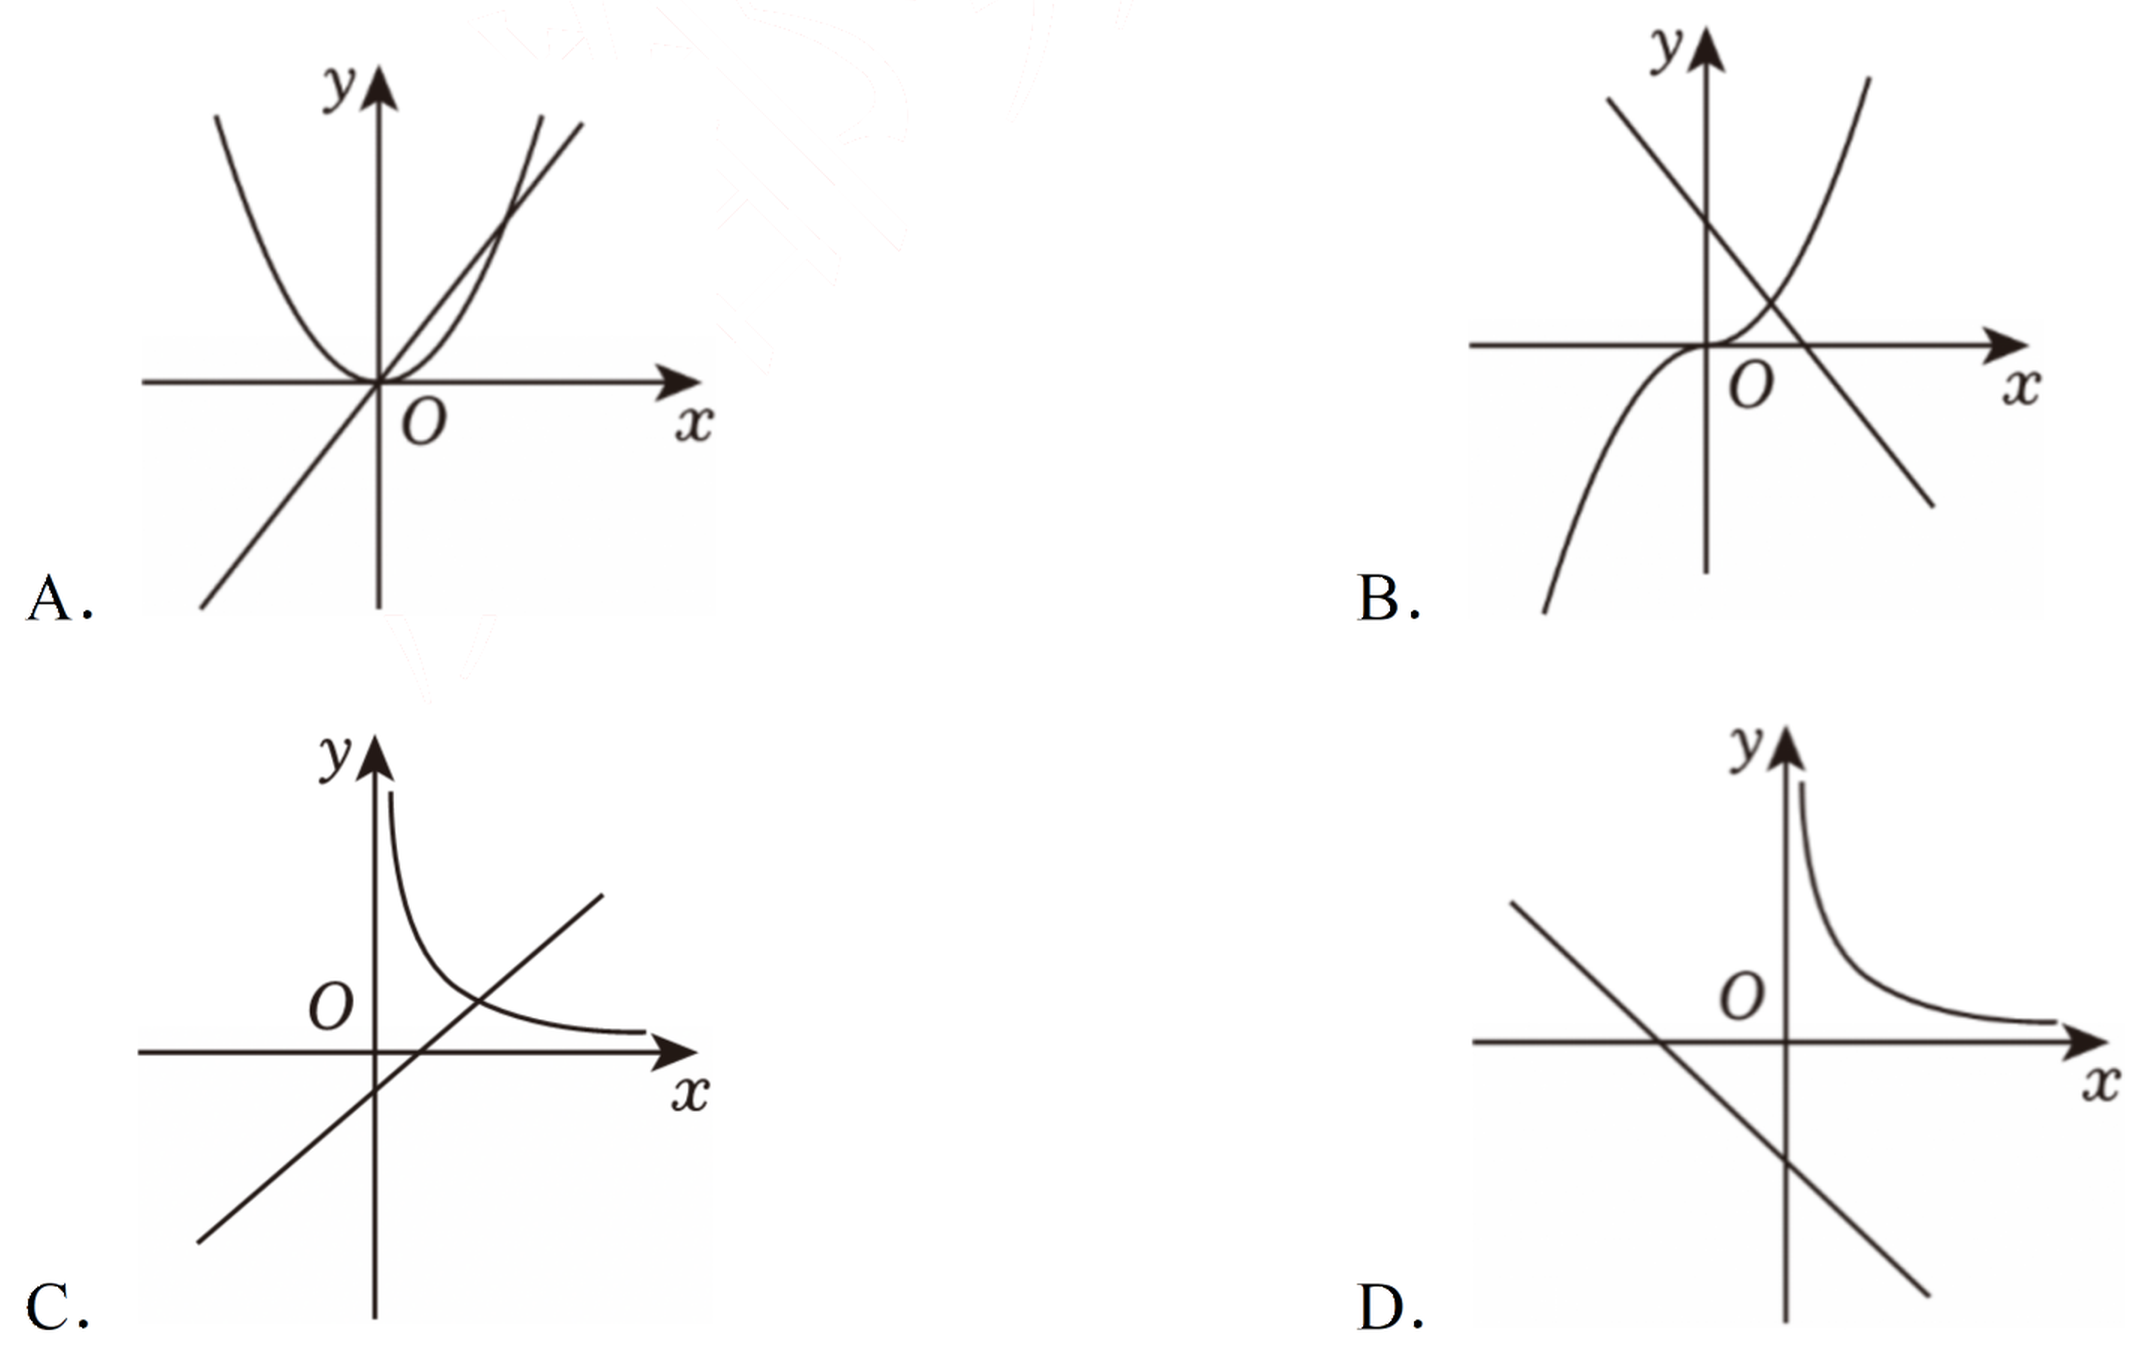
\includegraphics[width=0.80\textwidth]{figures/gao132_q14.png}
\end{center}

\ifanswer
\solbegin
\step{当 $a>0$ 时，$y=ax-\dfrac1a$ 严格增，当 $a<0$ 时，$y=ax-\dfrac1a$ 严格减，}
\step{对于 $A$，因为 $a\ne0$，所以直线 $y=ax-\dfrac1a$ 不过原点，故 $A$ 错误；}
\step{对于 $B$，由函数 $y=x^a(a\ne0)$ 的图象得 $a>1$，}
\step{由 $y=ax-\dfrac1a$ 的图象得 $a<0$，互相矛盾，故 $B$ 错误；}
\step{对于 $C$，由函数 $y=x^a(a\ne0)$ 的图象得 $a>1$，}
\step{由 $y=ax-\dfrac1a$ 的图象得 $a>0$ 且 $-\dfrac1a<0$，符合题意，故 $C$ 正确；}
\step{对于 $D$，由函数 $y=x^a(a\ne0)$ 的图象得 $a<0$，}
\step{由 $y=ax-\dfrac1a$ 的图象得 $a<0$ 且 $-\dfrac1a<0$，互相矛盾，故 $D$ 错误；}
\step{故选 $C$.}
\solend
\fi

\item 中国的 $5G$ 技术领先世界，在 $5G$ 技术中，最大数据传输速率 $C$ 取决于信道带宽 $W$，$C$ 与 $W$ 满足 $C=W\log_2\left(1+\dfrac SN\right)$，其中 $\dfrac SN$ 称为信噪比（单位：$dB$）. 若不改变带宽 $W$，初始信噪比 $\dfrac SN$ 为 $1000$，那么为了使 $C$ 增加 $30\%$，需要将信噪比 $\dfrac SN$ 从 $1000$ 提升至大约\mbox{（\quad）}

\keepwithprev
A. $5000$\qquad\qquad B. $6000$\qquad\qquad C. $7000$\qquad\qquad D. $8000$

\ifanswer
\solbegin
\step{由题意得 $\dfrac SN=1000$ 时，$C=W\log_2(1+1000)\approx W\log_2 1000$，}
\step{要使 $C$ 增加 $30\%$，则 $(1+30\%)C=W\log_2\left(1+\dfrac SN\right)$，即 $1.3C\approx W\log_2\dfrac SN$，}
\step{所以 $1.3\approx\log_{1000}\dfrac SN=\dfrac{\lg\frac SN}{\lg1000}$，所以 $\lg\dfrac SN=3.9$，所以 $\dfrac SN=10^{3.9}\approx8000$.}
\step{故选 $D$.}
\solend
\fi

\item 对于 $a\in\R$，设非空集合 $A=\left\{x\mid\dfrac{(x^2-930x+a)(x-52)}{x+a}=0\right\}$，记 $A$ 中的所有元素之和为 $S(a)$，所有元素之积为 $T(a)$，则下列说法中，不正确的是\mbox{（\quad）}

\keepwithprev
A. 存在实数 $a$，使得 $S(a)=930$

B. 存在实数 $a$，使得 $T(a)=517$

C. 不存在实数 $a$，使得 $T(a)=0$

D. 恰存在 $1$ 个实数 $a$，使得 $T(a)=-52$

\ifanswer
\solbegin
\step{由分式值为 $0$，得分子为 $0$ 且分母不为 $0$，}
\step{分子 $(x^2-930x+a)(x-52)=0$ 的根为 $x=52$}
\step{及方程 $x^2-930x+a=0$ 的两根 $x_1$，$x_2$，}
\step{由根与系数的关系得 $x_1+x_2=930$，$x_1\cdot x_2=a$，}
\step{分母限制 $x\ne-a$，需要剔除等于 $-a$ 的根，}
\step{选项 $A$，取 $a=-52$，$x=52$ 为增根舍去，集合 $A=\{x_1,x_2\}$，}
\step{元素之和 $S(a)=930$，故 $A$ 正确；}
\step{选项 $B$，当无增根时，$T(a)=52a$，令 $52a=517$，得 $a=\dfrac{517}{52}$，}
\step{验证无增根，存在这样的 $a$，故 $B$ 正确；}
\step{选项 $C$，若 $T(a)=0$，则 $0\in A$，代入分子得 $a=0$，}
\step{但 $a=0$ 时分母 $x\ne0$，$x=0$ 为增根，$0$ 不能属于集合 $A$，}
\step{故不存在 $a$ 使得 $T(a)=0$，故 $C$ 正确；}
\step{选项 $D$，当无增根时，令 $52a=-52$，得 $a=-1$；}
\step{当 $x=-a$ 是二次方程的根且不等于 $52$ 时，}
\step{令 $52\times(930+a)=-52$，解得 $a=-931$，验证符合条件；}
\step{当 $a=-52$ 时，$x=52$，舍去，}
\step{集合 $A=\{x_1,x_2\}$，$T(a)=a=-52$，得到两个满足条件的 $a$；}
\step{因此存在 $3$ 个满足条件的 $a$，故 $D$ 错误.}
\step{故选 $D$.}
\solend
\fi

\end{enumerate}

\bigsec{三、解答题}

\begin{enumerate}
\setcounter{enumi}{16}

\item 已知全集 $U=\R$，集合 $A=\left\{x\mid\dfrac{x}{x-3}<0\right\}$，$B=\{x\mid(x-a)(x+4-a)<0\}$.

(1) 当 $a=2$ 时，求 $\overline{B}$、$A\cap\overline{B}$；

(2) 若 $A\cap B=A$，求实数 $a$ 的取值范围.

\ifanswer
\solbegin
\step{(1) $\dfrac{x}{x-3}<0$，即 $x(x-3)<0$，解得 $A=\{x\mid0<x<3\}$，}
\step{当 $a=2$ 时，$B=\{x\mid(x-a)(x+4-a)<0\}=\{x\mid-2<x<2\}$，}
\step{则 $\overline{B}=\{x\mid x\leq-2$ 或 $x\geq2\}$，故 $A\cap\overline{B}=\{x\mid2\leq x<3\}$；}
\step{(2) $A\cap B=A$，则 $A\subseteq B$，故 $\begin{cases}a-4\leq0\\a\geq3\end{cases}$，解得 $3\leq a\leq4$，}
\step{故实数 $a$ 的取值范围是 $\{a\mid3\leq a\leq4\}$.}
\solend
\fi

% 第 18 题是"题干 + 图"约 7cm 的一整块，守卫放在 \item 之前
\needvspace{7cm}
\item 如图，$OA$、$OB$ 是两条长度足够长的互相垂直的笔直小路，矩形 $OCPD$ 的顶点 $C$、$D$ 分别在 $OA$、$OB$ 上，且该矩形区域内种满了荷花. 为了让观赏者有更好的观赏体验，现计划经过点 $P$ 修一条小路 $EF$，其中点 $E$ 在小路 $OA$ 上，点 $F$ 在小路 $OB$ 上，并在 $\triangle OEF$ 区域内种满荷花. 已知 $OD=25m$，$OC=40m$，且小路 $EF$ 要完全位于一个以 $O$ 为顶点的，边长为 $100$ m 的正方形内部（包括边界）. 记 $\triangle OEF$ 的面积为 $S$m$^2$.

(1) 设 $EC=x\cdot m$，试用 $x$ 表示 $OF$，并求 $x$ 的取值范围.

(2) 当 $EC$ 的长度为多少时，$S$ 取得最小值？最小值是多少？

\begin{center}
% 图取原卷 07 页截图去粉色水印，3× LANCZOS 放大
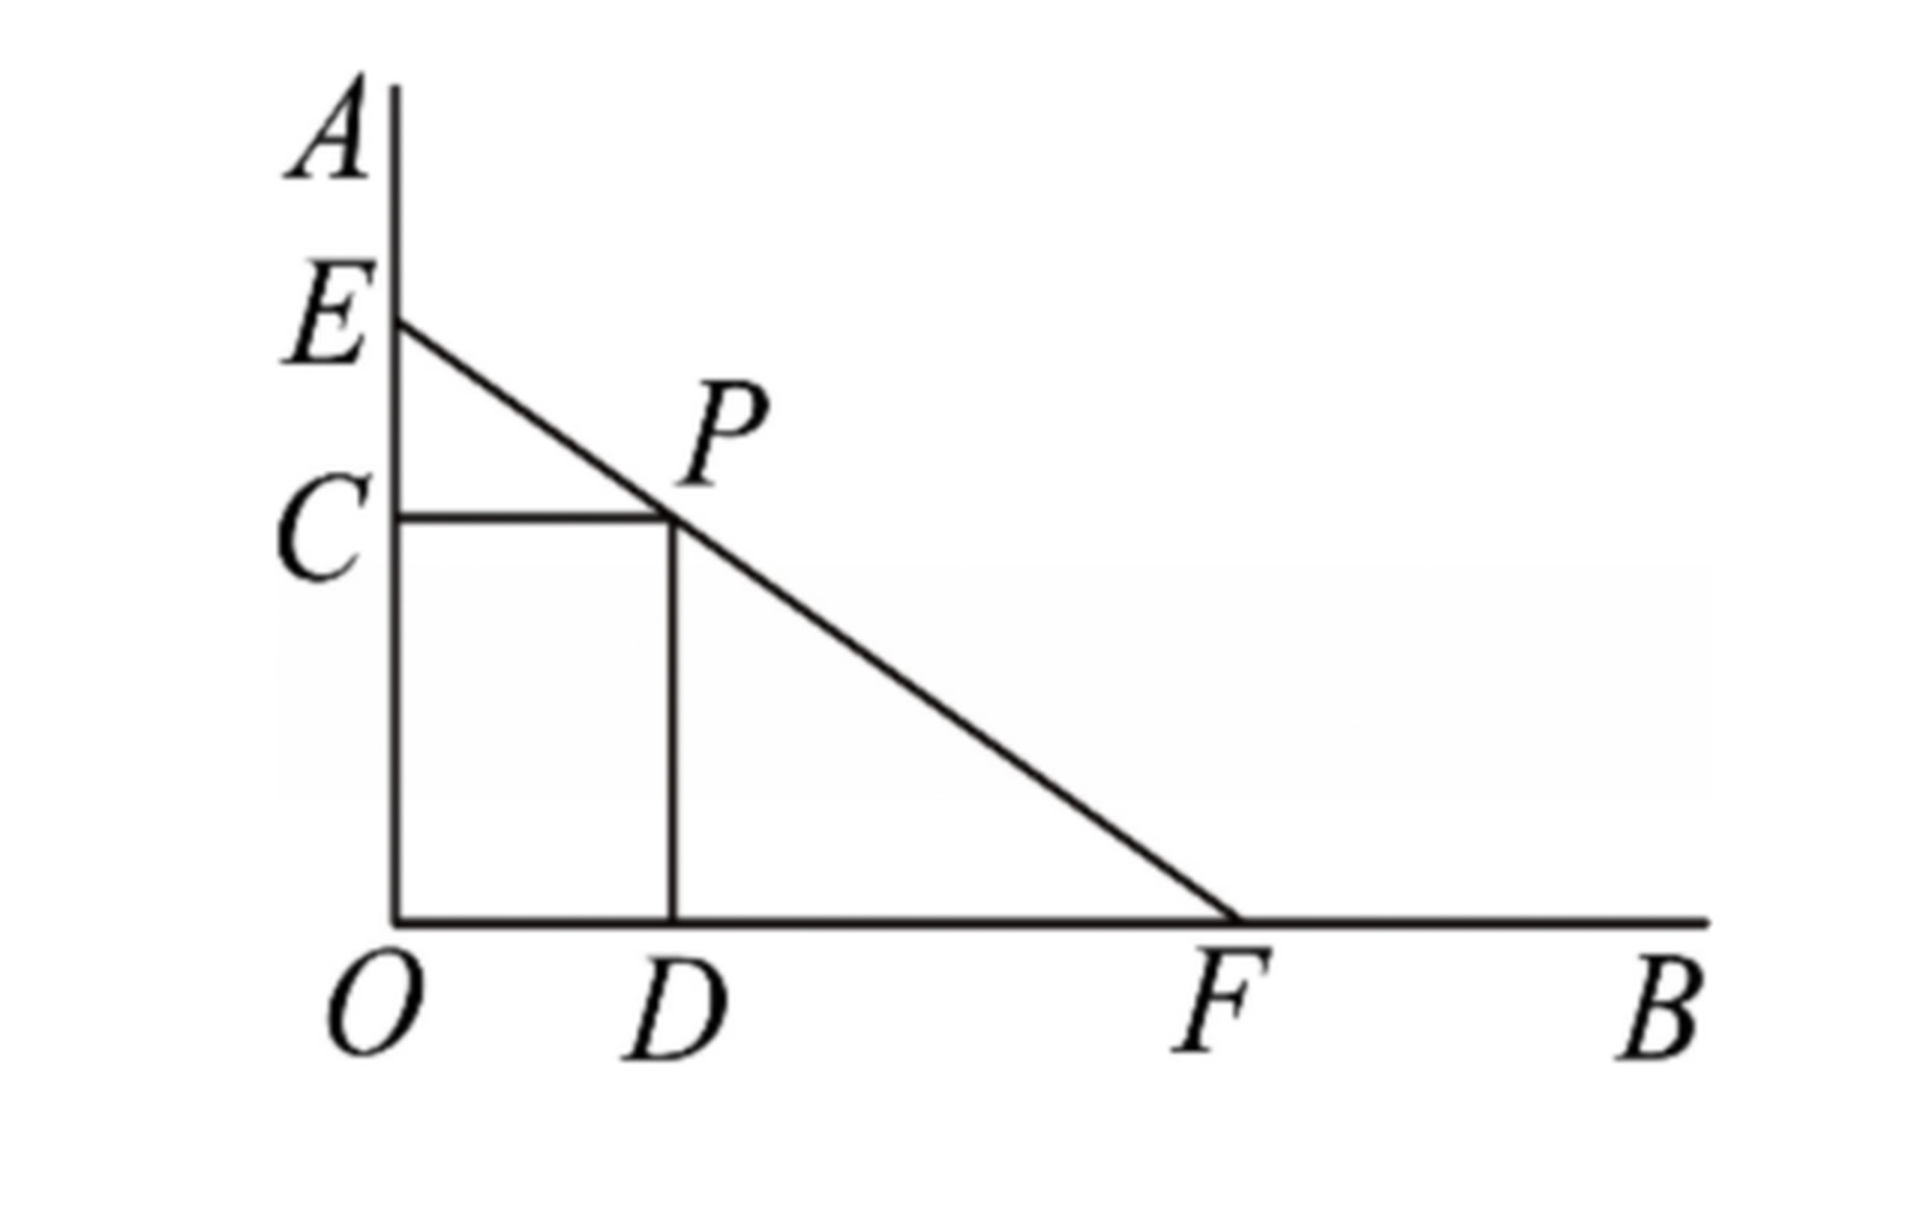
\includegraphics[width=0.32\textwidth]{figures/gao132_q18.png}
\end{center}

\ifanswer
\solbegin
\step{(1) 由题意得 $x\leq60$，}
\step{$\triangle PCE\sim\triangle FDP$，所以 $\dfrac{EC}{CP}=\dfrac{PD}{DF}$，即 $\dfrac{x}{25}=\dfrac{40}{DF}$，得 $DF=\dfrac{1000}{x}$m，}
\step{所以 $OF=OD+DF=\left(25+\dfrac{1000}x\right)$m，}
\step{所以 $25+\dfrac{1000}x\leq100$，解得 $x\geq\dfrac{40}3$；}
\step{综上，$\dfrac{40}3\leq x\leq60$；}
\step{(2) 由 $OE=OC+CE=(40+x)$m，}
\step{所以 $S=\dfrac12 OF\cdot OE=\dfrac12\left(25+\dfrac{1000}x\right)(40+x)$}
\step{$=\dfrac12\left(1000+25x+\dfrac{40000}x+1000\right)$m$^2$，}
\step{由基本不等式得 $S\geq\dfrac12\left(2000+2\sqrt{25x\cdot\dfrac{40000}x}\right)=2000$m$^2$，}
\step{当且仅当 $25x=\dfrac{40000}x$，即 $x=40$ 时取等号，}
\step{故 $EC=40$m 时，$S$ 取得最小值，为 $2000$m$^2$.}
\solend
\fi

\item 已知 $a>0$，$b>0$，请选择适当的方法证明.

(1) 若 $a\ne b$，证明：$a^3+b^3>a^2b+ab^2$；

(2) 若 $ab=1$，证明：$a^2+a<2$ 与 $b^2+b<2$ 不能同时成立.

\ifanswer
\solbegin
\step{(1) 因为 $a>0$，$b>0$，$a\ne b$，}
\step{所以 $a^3+b^3-a^2b-ab^2=a^2(a-b)+b^2(b-a)$}
\step{$=(a^2-b^2)(a-b)=(a-b)^2(a+b)>0$，所以 $a^3+b^3>a^2b+ab^2$.}
\step{(2) 假设 $a^2+a<2$ 与 $b^2+b<2$ 同时成立，所以 $-2<a<1,-2<b<1$，}
\step{又因为 $a>0,b>0$，所以 $0<a<1,0<b<1$，}
\step{所以 $0<ab<1$，这与 $ab=1$ 矛盾，}
\step{故 $a^2+a<2$ 与 $b^2+b<2$ 不可能同时成立.}
\solend
\fi

\item 若设 $M(a,n)=\lvert ax-1\rvert+\lvert ax-2\rvert+\cdots+\lvert ax-n\rvert$ 为曼哈顿扩张距离，它由 $n$ 个绝对值之和组成，其中 $n$ 为正整数.

(1) 若 $M(2,1)\leq5$，求 $x$ 的取值范围；

(2) 若 $k\leq M(2,2)$ 对一切实数 $x$ 恒成立，求实数 $k$ 的取值范围；

(3) $M(2,6)$ 是否存在最小值？若存在，求出该最小值与此时实数 $x$ 的取值范围；若不存在，说明理由.

\ifanswer
\solbegin
\step{(1) $M(2,1)=\lvert2x-1\rvert\leq5$，则不等式可化为 $-5\leq2x-1\leq5$，解得 $-2\leq x\leq3$，}
\step{所以 $x$ 的取值范围为 $[-2,3]$.}
\step{(2) 因为 $k\leq M(2,2)=\lvert2x-1\rvert+\lvert2x-2\rvert$ 对一切实数 $x$ 恒成立，}
\step{又 $\lvert2x-1\rvert+\lvert2x-2\rvert\geq\lvert(2x-1)-(2x-2)\rvert=1$，}
\step{当且仅当 $(2x-1)(2x-2)\leq0$，即 $\dfrac12\leq x\leq1$ 时取等号，}
\step{故 $k\leq1$，所以实数 $k$ 的取值范围为 $(-\infty,1]$.}
\step{(3) $M(2,6)=\lvert2x-1\rvert+\lvert2x-2\rvert+\lvert2x-3\rvert+\lvert2x-4\rvert+\lvert2x-5\rvert+\lvert2x-6\rvert$}
\step{$=2\left(\left\lvert x-\dfrac12\right\rvert+\lvert x-1\rvert+\left\lvert x-\dfrac32\right\rvert+\lvert x-2\rvert+\left\lvert x-\dfrac52\right\rvert+\lvert x-3\rvert\right)$，}
\step{其中 $\left\lvert x-\dfrac12\right\rvert+\lvert x-1\rvert+\left\lvert x-\dfrac32\right\rvert+\lvert x-2\rvert+\left\lvert x-\dfrac52\right\rvert+\lvert x-3\rvert$ 的几何意义为}
\step{在数轴上一点 $x$ 到 $\dfrac12,1,\dfrac32,2,\dfrac52,3$ 的距离之和，}
\step{要想距离之和最小，其中 $x\in\left[\dfrac12,3\right]$ 时，$\left\lvert x-\dfrac12\right\rvert+\lvert x-3\rvert$ 取得最小值，}
\step{当 $x\in\left[1,\dfrac52\right]$ 时，$\lvert x-1\rvert+\left\lvert x-\dfrac52\right\rvert$ 取得最小值，}
\step{当 $x\in\left[\dfrac32,2\right]$ 时，$\left\lvert x-\dfrac32\right\rvert+\lvert x-2\rvert$ 取得最小值，}
\step{综上，当 $x\in\left[\dfrac32,2\right]$ 时，$\left\lvert x-\dfrac12\right\rvert+\lvert x-1\rvert+\left\lvert x-\dfrac32\right\rvert+\lvert x-2\rvert+\left\lvert x-\dfrac52\right\rvert+\lvert x-3\rvert$}
\step{取得最小值，最小值为 $3-\dfrac12+\dfrac52-1+2-\dfrac32=\dfrac92$，}
\step{故 $M(2,6)=2\left(\left\lvert x-\dfrac12\right\rvert+\lvert x-1\rvert+\left\lvert x-\dfrac32\right\rvert+\lvert x-2\rvert+\left\lvert x-\dfrac52\right\rvert+\lvert x-3\rvert\right)$ 的}
\step{最小值为 $9$.}
\solend
\fi

\item 已知集合 $A=\{a_1,a_2,\cdots,a_n\}(0\leq a_1<a_2<\cdots<a_n,n\in\N,n\geq3)$ 具有性质 $Q$：对任意 $i,j(1\leq i\leq j\leq n)$，$a_i+a_j$ 与 $a_j-a_i$ 至少有一个属于集合 $A$；

(1) 判断集合 $M=\{0,2,4\}$ 与 $N=\{2,3,4\}$ 是否具有性质 $Q$，并说明理由；

(2) 已知 $A=\{a_1,a_2,a_3\}$ 具有性质 $Q$，当 $a_2=2026$ 时，求集合 $A$；

(3) 已知 $B=\{b_1,b_2,\cdots,b_{2026}\}$ 具有性质 $Q$，求 $\dfrac{b_1+b_2+\cdots+b_{2026}}{b_{2026}}$ 的值；

\ifanswer
\solbegin
\step{(1) 集合 $M=\{0,2,4\}$ 中，}
\step{因为 $0+2\in M,0+4\in M,4-2\in M,0\pm0=0\in M$，}
\step{$2+2=4\in M,2-2=0\in M,4-4=0\in M$，所以集合 $M$ 具有性质 $Q$；}
\step{集合 $N=\{2,3,4\}$ 中，因为 $3+3=6\notin N,3-3=0\notin N$，}
\step{所以集合 $N$ 不具有性质 $Q$.}
\step{(2) 因为 $a_1<a_2<a_3$，且 $A=\{a_1,a_2,a_3\}$ 具有性质 $Q$，}
\step{所以 $a_3+a_3\notin A,a_3-a_3=0\in A$，则 $a_1=0$，}
\step{又因为 $a_2+a_3>a_3$，所以 $a_2+a_3\notin A$，则 $a_3-a_2\in A$，}
\step{由集合的互异性得 $a_3-a_2=a_2$，而 $a_2=2026$，所以 $a_3=4052$，}
\step{故 $A=\{0,2026,4052\}$；}
\step{(3) 先证明一般结论：$A=\{a_1,a_2,\cdots,a_n\}(0\leq a_1<a_2<\cdots<a_n,n\in\N,n\geq3)$}
\step{具有性质 $Q$，则 $a_1+a_2+a_3+\cdots+a_n=\dfrac n2 a_n$.}
\step{因为 $A=\{a_1,a_2,\cdots,a_n\}(0\leq a_1<a_2<\cdots<a_n,n\in\N,n\geq3)$ 具有性质 $Q$，}
\step{所以 $a_n+a_n\notin A$，则 $a_n-a_n=0\in A$，则 $a_1=0$.}
\step{又因为 $0\leq a_1<a_2<\cdots<a_n$，所以 $0\leq a_n-a_n<a_n-a_{n-1}<\cdots<a_n-a_1$，}
\step{又因为 $a_n+a_{n-i}>a_n(i=1,2,\cdots,n-1)$，所以 $a_n+a_{n-i}\notin A$，}
\step{则 $a_n-a_{n-i}\in A$，}
\step{所以 $a_1=a_n-a_n,a_2=a_n-a_{n-1},a_3=a_n-a_{n-2},\cdots,a_n=a_n-a_1$.}
\step{所以 $a_1+a_2+a_3+\cdots+a_n$}
\step{$=(a_n-a_n)+(a_n-a_{n-1})+(a_n-a_{n-2})+\cdots+(a_n-a_1)$，}
\step{即 $a_1+a_2+a_3+\cdots+a_n=\dfrac n2 a_n$，}
\step{所以 $B=\{b_1,b_2,\cdots,b_{2026}\}$ 具有性质 $Q$，则 $b_1+b_2+\cdots+b_{2026}=\dfrac{2026}{2}b_{2026}$，}
\step{所以 $\dfrac{b_1+b_2+\cdots+b_{2026}}{b_{2026}}=\dfrac{2026}{2}=1013$.}
\solend
\fi

\end{enumerate}

% 行数复核：逐题数 \step 条数，合计 144 条（Q3：4；Q4：1；Q5：4；Q6：2；Q7：9；Q8：2；
% Q9：3；Q10：6；Q11：9；Q12：9；Q13：0；Q14：9；Q15：4；Q16：19；Q17：5；Q18：11；
% Q19：7；Q20：17；Q21：23），与原卷印刷行逐题相等（cases 块作一个印刷行计）。
% 第 13 题只印括号内答案、提 \ans{}，不计入 \step 账；第 14—16 题答案在解析末句，
% 括号内留空、不另提 \ans{}。

\end{document}
"
%
% 原始材料：微信公众号"魔都数学加油站"文章，作者破晓，2026-11-14 19:00 发布；
% 连载"27学年高一132"，原文标题"27学年高一132——2026-2027年上海市川沙中学高一上期中"；
% 原文链接：https://mp.weixin.qq.com/s/VBG01CrUNMIYWWHhSfz8JQ。
% 正文为 11 张 PNG 页（01、04、06、07、09、11 为 2560x3620，02、03、05、08、10 为 4762x6735），
% 题目下印有【解析】，为讲评版。题目、解析均据原图转录；
% 卷面粉红色水印"魔都数学加油站"及公众号页脚未录入。全卷 2 幅插图：第 14 题四幅坐标图选项、
% 第 18 题矩形 OCPD 与小路 EF 示意图，均取原卷 04／07 页截图去水印。
%
% 卷首标题：原卷印作"2026-2027 年川沙中学高一上期中"（公众号标题中的"上海市"
% 卷面标题行没有，本稿照卷面），年份区间按全稿惯例排 en dash；原卷未印副标题，
% 本卷为期中卷、跨集合与常用逻辑用语／不等式／函数三章，按题目内容标为
% "集合与常用逻辑用语、不等式、函数"（与 125／126／128／129／131 同期中卷口径相同）：
% 集合与逻辑见 Q5、Q6、Q17、Q21，不等式见 Q3、Q4、Q9、Q10、Q12、Q13、Q15、Q16、Q19，
% 函数（幂函数、指数／对数、基本不等式应用）见 Q7、Q8、Q11、Q14、Q18、Q20。
%
% 题号体例：本卷共 19 题——一、填空题 3—12（10 题）、二、选择题 13—16（4 题）、
% 三、解答题 17—21（5 题）。三节分别 \setcounter{enumi}{2}／{12}／{16}。
%
% 与原卷的排版差异：
%   ① 原文从第 3 题起，本稿保留原题号（见上"题号体例"）；
%   ② 原卷每题下直接印【解析】，本稿按全稿惯例置于答案版；第 13 题答案 D 印在题干
%      括号内、无独立答案段，按 高一37／52／53／55／63／64／128／131 成例括号留空、
%      另提 \ans{$D$}；第 14—16 题答案在解析末句"故选 …"，括号内留空、不另提 \ans{}；
%   ③ 原卷未印副标题，本稿按"知识模块"口径补出；
%   ④ 原卷填空横线按全稿惯例排为 \blankline[4.4em]；选择题括号排 \mbox{（\quad）}、
%      选项段前按惯例加 \keepwithprev；解答题不留作答区（原卷为讲评版，与 109—131 同）；
%   ⑤ 原卷数集排斜体 $R^+$／$R$／$Z$／$N$，按全稿惯例改 \R^+／\R／\Z／\N；
%      绝对值排 \lvert…\rvert，集合描述竖线排 \mid；不等号按全稿惯例排 \leqslant／\geqslant；
%      补集照原卷上划线排 \overline{B}；
%   ⑥ 子题标号 (1)(2)(3) 原卷用半角括号，照录；第 14 题四幅坐标图选项按原卷 2×2 排布
%      合并裁为一张 \includegraphics（未用 TikZ 重绘，以保证与原卷一致），题前加
%      \needvspace{9cm} 守卫；第 18 题图取 07 页截图，题前按惯例加 \needvspace{7cm} 守卫
%      （照 高一120／127／129／131 成例），两者守卫都放在 \item 之前；
%   ⑦ 原卷 Q7 解析跨 01—02 页、Q10 解析跨 02—03 页、Q12 解析跨 03—04 页、
%      Q14 解析跨 04—05 页、Q16 解析在 06 页、Q18 解析跨 07—08 页、
%      Q20 解析跨 08—09 页、Q21 解析跨 10—11 页，本稿按题合并连续排版；
%      末页第 11 页为 Q21 (3) 解析的续尾，按实际印刷行单列。
%
% 判别式字形：第 10 题 $\triangle=4(a-1)^2+16(a-1)<0$、第 11 题
%   $\triangle=4(m-2)^2-4(m^2-3m+3)=-4m+4>0$ 两处原卷均排 $\triangle$（等边、扁），
%   逐处放大核对、字形一致，照录 \triangle；与 高一129／131 同题排 $\Delta$（等腰、高）不同。
%   全卷 \triangle 兼作第 18 题「$\triangle PCE\sim\triangle FDP$」「$\triangle OEF$」的几何
%   三角形记号，全卷未出现 \Delta。
%
% 子集符号：第 5 题解析 $B\subseteq A$、第 17 题 (2) 解析 $A\subseteq B$ 均印带下划线，
%   照录 \subseteq；全卷未出现单线 \subset。
%
% 原卷存疑照录：
%   第 9 题题干作"充分非必要条件"、解析作"充分不必要条件"，措辞不同，照录；
%   第 10 题解析"当 $a-1=0$ 时，$-4\geq0$，不等式不成立，$a=1$ 满足题意"照录；
%   第 11 题解析"所以 $2(m-1)+\dfrac1{m-1}\leq-2\sqrt2$"由上一行 $2(1-m)+\dfrac1{1-m}\geq2\sqrt2$
%     直接变号得到，照录；
%   第 12 题解析"由 $x\in Z$，$-7<-2\sqrt{10}<-6$"与"即 $k^2+7k+10\leq0$，解得 $-5\leq k\leq-2$"照录；
%   第 16 题解析"令 $52\times(930+a)=-52$，解得 $a=-931$"（按式应为 $a=-931$ 之外的解）照录；
%   第 19 题 (2) 解析"所以 $-2<a<1,-2<b<1$"数学式内半角逗号，照录；
%   第 20 题 (3) 解析"最小值为 $3-\dfrac12+\dfrac52-1+2-\dfrac32=\dfrac92$"与
%     "故 $M(2,6)=\dots$ 的最小值为 9"两处结论并列，照录；
%   第 21 题 (1) 解析"$0+2\in M,0+4\in M,4-2\in M,0\pm0=0\in M$"、
%     "$2+2=4\in M,2-2=0\in M,4-4=0\in M$"、(3) 各连写等式内半角逗号，照录；
%   第 21 题 (3) 解析"即 $a_1+a_2+a_3+\cdots+a_n=\dfrac n2 a_n$，"句末用半角逗号，照录。
%
% 行数复核：见文末"行数复核"注（逐题 \step 条数与原卷印刷行逐题相等，cases 块作一个印刷行计）。
%   第 13 题只印括号内答案、提 \ans{}，不计入 \step 账；第 14—16 题答案在解析末句，
%   括号内留空、不另提 \ans{}。
%
\documentclass[a4paper,11pt]{article}
\usepackage{common}

\begin{document}

\examtitlest[3]{2026--2027 年川沙中学高一上期中}{集合与常用逻辑用语、不等式、函数}

\bigsec{一、填空题}

\begin{enumerate}
\setcounter{enumi}{2}

\item 已知 $a$、$b\in\R^+$ 且 $ab=2$，则 $a+2b$ 的最小值为\blankline[4.4em].

\ifanswer
\solbegin
\step{因为 $a\in\R^+$，$b\in\R^+$ 且 $ab=2$，}
\step{由基本不等式得 $a+2b\geq2\sqrt{a\cdot2b}=2\sqrt{2ab}=2\sqrt4=4$.}
\step{等号当且仅当 $a=2b$ 时成立，结合 $ab=2$ 解得 $b=1$，$a=2$，}
\step{所以 $a+2b$ 的最小值为 $4$.}
\solend
\fi

\item 如果幂函数 $f(x)=(m^2-3m-3)x^{m^2+m-3}$ 在 $(0,+\infty)$ 上是增函数，则实数 $m=$\blankline[4.4em].

\ifanswer
\solbegin
\step{由已知得 $\begin{cases}m^2-3m-3=1\\m^2+m-3>0\end{cases}$，所以 $m=4$.}
\solend
\fi

\item 已知集合 $A=\{1,2\}$，集合 $B=\{x\mid ax=6\}$，若 $A\cup B=A$，则 $a$ 的所有取值构成的集合为\blankline[4.4em].

\ifanswer
\solbegin
\step{因为 $A\cup B=A$，所以 $B\subseteq A$，}
\step{当 $a=0$ 时，$B=\varnothing$，满足 $B\subseteq A$；}
\step{当 $a\ne0$ 时，$B=\left\{\dfrac6a\right\}$，则 $\dfrac6a=1$ 或 $\dfrac6a=2$，解得 $a=6$ 或 $a=3$，}
\step{综上所述，$a$ 的所有取值构成的集合为 $\{0,3,6\}$.}
\solend
\fi

\item 设全集为 $\R$，$A=\{y\mid y=-x^2+2x+1\}$，$B=\{x\mid y=\ln(x-1)\}$，则 $A\cap B=$\blankline[4.4em].

\ifanswer
\solbegin
\step{$A=\{y\mid y=-x^2+2x+1\}=\{y\mid y=-(x-1)^2+2\}=\{y\mid y\leq2\}$，}
\step{$B=\{x\mid y=\ln(x-1)\}=\{x\mid x>1\}$，则 $A\cap B=(1,2]$.}
\solend
\fi

\item 已知 $x\in\R$，则方程 $\lvert 6-x\rvert+\lvert 6x-3\rvert=\lvert 5x+3\rvert$ 的解集为\blankline[4.4em].

\ifanswer
\solbegin
\step{当 $x<-\dfrac35$ 时，$6-x>0$，$6x-3<0$，$5x+3<0$，}
\step{原方程为 $6-x-6x+3=-5x-3$，解得 $x=6$，不满足 $x<-\dfrac35$；}
\step{当 $-\dfrac35\leq x\leq\dfrac12$ 时，$5x+3\geq0$，$6x-3<0$，$6-x>0$，}
\step{原方程为 $6-x+3-6x=5x+3$，解得 $x=\dfrac12$；}
\step{当 $\dfrac12<x\leq6$ 时，$5x+3>0$，$6x-3>0$，$6-x\geq0$，}
\step{原方程为 $6-x+6x-3=5x+3$，即 $0=0$，恒成立，所以 $\dfrac12<x\leq6$；}
\step{当 $x>6$ 时，$5x+3\geq0$，$6x-3>0$，$6-x<0$，}
\step{原方程为 $x-6+6x-3=5x+3$，解得 $x=6$，不满足 $x>6$；}
\step{综上 $\dfrac12\leq x\leq6$，所以原方程的解集为 $\left\{x\mid\dfrac12\leq x\leq6\right\}$.}
\solend
\fi

\item 已知 $\log_2 3=a,2^b=7$，用 $a,b$ 表示 $\log_{42}56$ 为\blankline[4.4em].

\ifanswer
\solbegin
\step{$\log_{42}56=\dfrac{\log_2 56}{\log_2 42}=\dfrac{\log_2(7\times8)}{\log_2(6\times7)}=\dfrac{\log_2 7+\log_2 8}{\log_2 6+\log_2 7}$}
\step{$=\dfrac{\log_2 7+\log_2 2^3}{\log_2 2+\log_2 3+\log_2 7}=\dfrac{b+3}{1+a+b}$.}
\solend
\fi

\item 已知 $\dfrac13<x<\dfrac12$ 是不等式 $\lvert x-m\rvert<1$ 成立的充分非必要条件，则 $m$ 的取值范围是\blankline[4.4em].

\ifanswer
\solbegin
\step{因为 $\lvert x-m\rvert<1$，所以 $-1<x-m<1$，所以 $m-1<x<m+1$，}
\step{所以 $m-1<x<m+1$ 成立的充分不必要条件是 $\dfrac13<x<\dfrac12$，}
\step{所以 $\begin{cases}m-1\leq\dfrac13\\m+1\geq\dfrac12\end{cases}$，解得 $-\dfrac12\leq m\leq\dfrac43$，故 $m$ 的取值范围是 $\left[-\dfrac12,\dfrac43\right]$.}
\solend
\fi

\item 若关于 $x$ 的不等式 $(a-1)x^2+2(a-1)x-4\geq0$ 的解集为空集，则 $a$ 的取值范围是\blankline[4.4em].

\ifanswer
\solbegin
\step{关于 $x$ 的不等式 $(a-1)x^2+2(a-1)x-4\geq0$ 的解集为 $\varnothing$，}
\step{当 $a-1=0$ 时，$-4\geq0$，不等式不成立，$a=1$ 满足题意；}
\step{当 $a-1>0$ 时，$a>1$，不等式的解集不为空集，不满足题意；}
\step{当 $a-1<0$ 时，$a<1$，当 $\triangle=4(a-1)^2+16(a-1)<0$ 时，即 $(a-1)(a+3)<0$，}
\step{解得 $-3<a<1$，满足题意；}
\step{综上，实数 $a$ 的取值范围是 $\{a\mid-3<a\leq1\}$.}
\solend
\fi

\item 已知关于 $x$ 的方程 $x^2+2(m-2)x+m^2-3m+3=0$ 有两个不相等的实数根 $x_1$、$x_2$，则 $\dfrac{mx_1}{x_1-1}+\dfrac{mx_2}{x_2-1}-\dfrac{2}{x_1+x_2-2}$ 的最大值为\blankline[4.4em].

\ifanswer
\solbegin
\step{关于 $x$ 的方程 $x^2+2(m-2)x+m^2-3m+3=0$ 有两个不相等的实数根 $x_1$、$x_2$，}
\step{则 $\triangle=4(m-2)^2-4(m^2-3m+3)=-4m+4>0$，得 $m<1$，}
\step{且 $x_1+x_2=-2(m-2)$，$x_1x_2=m^2-3m+3$，}
\step{$\dfrac{mx_1}{x_1-1}+\dfrac{mx_2}{x_2-1}-\dfrac{2}{x_1+x_2-2}=\dfrac{m[2x_1x_2-(x_1+x_2)]}{x_1x_2-(x_1+x_2)+1}+\dfrac1{m-1}$}
\step{$=\dfrac{2m(m-1)^2}{m^2-m}+\dfrac1{m-1}=2(m-1)+\dfrac1{m-1}$，}
\step{又因为 $m<1$，所以 $m-1<0$，则 $1-m>0$，}
\step{所以 $2(1-m)+\dfrac1{1-m}\geq2\sqrt{2(1-m)\cdot\dfrac1{1-m}}=2\sqrt2$，}
\step{当且仅当 $2(1-m)=\dfrac1{1-m}$ 时，即 $m=1-\dfrac{\sqrt2}2$ 时取等号，}
\step{所以 $2(m-1)+\dfrac1{m-1}\leq-2\sqrt2$，即 $\dfrac{mx_1}{x_1-1}+\dfrac{mx_2}{x_2-1}-\dfrac2{x_1+x_2-2}$ 的最大值为 $-2\sqrt2$.}
\solend
\fi

\item 若使集合 $A=\{x\mid(kx-k^2-10)(x-1)>0,x\in\Z\}$ 中的元素个数最少，则实数 $k$ 的取值范围是\blankline[4.4em].

\ifanswer
\solbegin
\step{由题意集合 $A=\{x\mid(kx-k^2-10)(x-1)>0,\ x\in\Z\}$，}
\step{$k=0$ 时，不等式解得 $x<1$，有无数个整数解；}
\step{$k\ne0$ 时，则不等式变形为 $k\left(x-k-\dfrac{10}k\right)(x-1)>0$，}
\step{当 $k>0$ 时，$k+\dfrac{10}k\geq2\sqrt{10}$，仅当 $k=\sqrt{10}$ 时等号成立，}
\step{此时不等式解得 $x>k+\dfrac{10}k$ 或 $x<1$，有无数个整数解；}
\step{当 $k<0$ 时，$k+\dfrac{10}k=-\left[(-k)+\left(-\dfrac{10}k\right)\right]\leq-2\sqrt{10}$，仅当 $k=-\sqrt{10}$ 时等号成立，}
\step{此时不等式解得 $k+\dfrac{10}k<x<1$，}
\step{由 $x\in\Z$，$-7<-2\sqrt{10}<-6$，要使集合 $A$ 中的元素最少，则 $k+\dfrac{10}k\geq-7$，}
\step{即 $k^2+7k+10\leq0$，解得 $-5\leq k\leq-2$，故实数 $k$ 的取值范围是 $[-5,-2]$.}
\solend
\fi

\end{enumerate}

\bigsec{二、选择题}

\begin{enumerate}
\setcounter{enumi}{12}

\item 下列说法正确的是\mbox{（\quad）}

\keepwithprev
A. 若 $a>b$，则 $\dfrac1a<\dfrac1b$\qquad\qquad B. 若 $a>b$，$c>d$，则 $ac>bd$

C. 若 $a>b$，则 $ac^2>bc^2$\qquad\qquad D. 若 $ac^2>bc^2$，则 $a>b$

\ifanswer
\ans{$D$}
\fi

% 第 14 题四幅坐标图选项是一整块，守卫放在 \item 之前
\needvspace{9cm}
\item 在同一坐标系内，函数 $y=x^a(a\ne0)$ 和 $y=ax-\dfrac1a$ 的图象可能是\mbox{（\quad）}

\keepwithprev
\begin{center}
% 四幅坐标图选项取原卷 04 页截图去粉色水印，按原卷 2×2 排布合并为一张
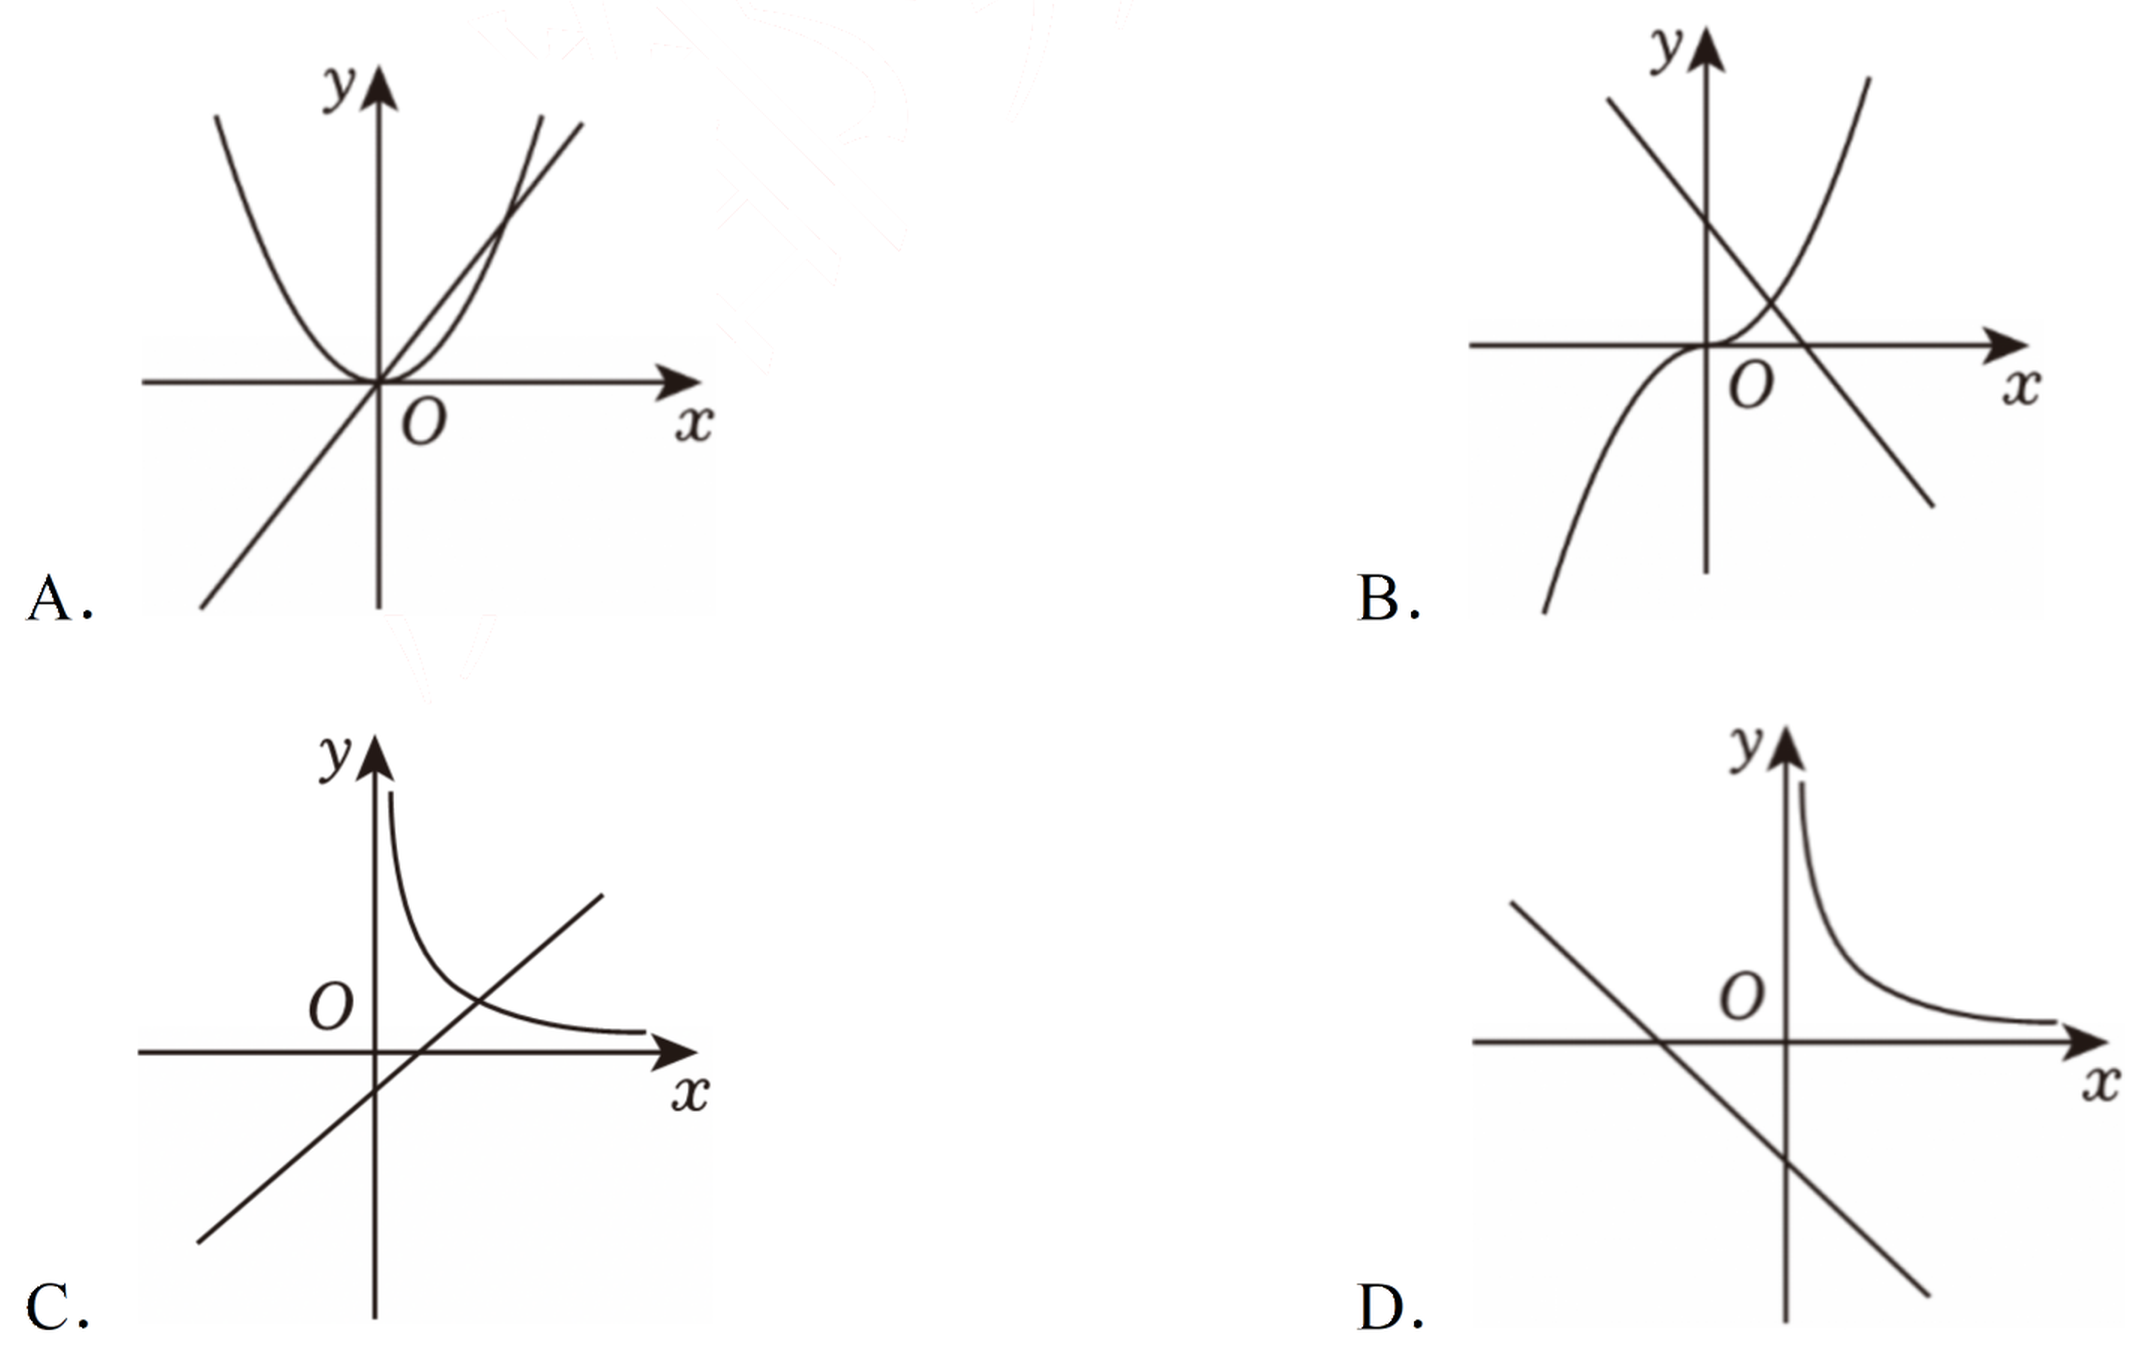
\includegraphics[width=0.80\textwidth]{figures/gao132_q14.png}
\end{center}

\ifanswer
\solbegin
\step{当 $a>0$ 时，$y=ax-\dfrac1a$ 严格增，当 $a<0$ 时，$y=ax-\dfrac1a$ 严格减，}
\step{对于 $A$，因为 $a\ne0$，所以直线 $y=ax-\dfrac1a$ 不过原点，故 $A$ 错误；}
\step{对于 $B$，由函数 $y=x^a(a\ne0)$ 的图象得 $a>1$，}
\step{由 $y=ax-\dfrac1a$ 的图象得 $a<0$，互相矛盾，故 $B$ 错误；}
\step{对于 $C$，由函数 $y=x^a(a\ne0)$ 的图象得 $a>1$，}
\step{由 $y=ax-\dfrac1a$ 的图象得 $a>0$ 且 $-\dfrac1a<0$，符合题意，故 $C$ 正确；}
\step{对于 $D$，由函数 $y=x^a(a\ne0)$ 的图象得 $a<0$，}
\step{由 $y=ax-\dfrac1a$ 的图象得 $a<0$ 且 $-\dfrac1a<0$，互相矛盾，故 $D$ 错误；}
\step{故选 $C$.}
\solend
\fi

\item 中国的 $5G$ 技术领先世界，在 $5G$ 技术中，最大数据传输速率 $C$ 取决于信道带宽 $W$，$C$ 与 $W$ 满足 $C=W\log_2\left(1+\dfrac SN\right)$，其中 $\dfrac SN$ 称为信噪比（单位：$dB$）. 若不改变带宽 $W$，初始信噪比 $\dfrac SN$ 为 $1000$，那么为了使 $C$ 增加 $30\%$，需要将信噪比 $\dfrac SN$ 从 $1000$ 提升至大约\mbox{（\quad）}

\keepwithprev
A. $5000$\qquad\qquad B. $6000$\qquad\qquad C. $7000$\qquad\qquad D. $8000$

\ifanswer
\solbegin
\step{由题意得 $\dfrac SN=1000$ 时，$C=W\log_2(1+1000)\approx W\log_2 1000$，}
\step{要使 $C$ 增加 $30\%$，则 $(1+30\%)C=W\log_2\left(1+\dfrac SN\right)$，即 $1.3C\approx W\log_2\dfrac SN$，}
\step{所以 $1.3\approx\log_{1000}\dfrac SN=\dfrac{\lg\frac SN}{\lg1000}$，所以 $\lg\dfrac SN=3.9$，所以 $\dfrac SN=10^{3.9}\approx8000$.}
\step{故选 $D$.}
\solend
\fi

\item 对于 $a\in\R$，设非空集合 $A=\left\{x\mid\dfrac{(x^2-930x+a)(x-52)}{x+a}=0\right\}$，记 $A$ 中的所有元素之和为 $S(a)$，所有元素之积为 $T(a)$，则下列说法中，不正确的是\mbox{（\quad）}

\keepwithprev
A. 存在实数 $a$，使得 $S(a)=930$

B. 存在实数 $a$，使得 $T(a)=517$

C. 不存在实数 $a$，使得 $T(a)=0$

D. 恰存在 $1$ 个实数 $a$，使得 $T(a)=-52$

\ifanswer
\solbegin
\step{由分式值为 $0$，得分子为 $0$ 且分母不为 $0$，}
\step{分子 $(x^2-930x+a)(x-52)=0$ 的根为 $x=52$}
\step{及方程 $x^2-930x+a=0$ 的两根 $x_1$，$x_2$，}
\step{由根与系数的关系得 $x_1+x_2=930$，$x_1\cdot x_2=a$，}
\step{分母限制 $x\ne-a$，需要剔除等于 $-a$ 的根，}
\step{选项 $A$，取 $a=-52$，$x=52$ 为增根舍去，集合 $A=\{x_1,x_2\}$，}
\step{元素之和 $S(a)=930$，故 $A$ 正确；}
\step{选项 $B$，当无增根时，$T(a)=52a$，令 $52a=517$，得 $a=\dfrac{517}{52}$，}
\step{验证无增根，存在这样的 $a$，故 $B$ 正确；}
\step{选项 $C$，若 $T(a)=0$，则 $0\in A$，代入分子得 $a=0$，}
\step{但 $a=0$ 时分母 $x\ne0$，$x=0$ 为增根，$0$ 不能属于集合 $A$，}
\step{故不存在 $a$ 使得 $T(a)=0$，故 $C$ 正确；}
\step{选项 $D$，当无增根时，令 $52a=-52$，得 $a=-1$；}
\step{当 $x=-a$ 是二次方程的根且不等于 $52$ 时，}
\step{令 $52\times(930+a)=-52$，解得 $a=-931$，验证符合条件；}
\step{当 $a=-52$ 时，$x=52$，舍去，}
\step{集合 $A=\{x_1,x_2\}$，$T(a)=a=-52$，得到两个满足条件的 $a$；}
\step{因此存在 $3$ 个满足条件的 $a$，故 $D$ 错误.}
\step{故选 $D$.}
\solend
\fi

\end{enumerate}

\bigsec{三、解答题}

\begin{enumerate}
\setcounter{enumi}{16}

\item 已知全集 $U=\R$，集合 $A=\left\{x\mid\dfrac{x}{x-3}<0\right\}$，$B=\{x\mid(x-a)(x+4-a)<0\}$.

(1) 当 $a=2$ 时，求 $\overline{B}$、$A\cap\overline{B}$；

(2) 若 $A\cap B=A$，求实数 $a$ 的取值范围.

\ifanswer
\solbegin
\step{(1) $\dfrac{x}{x-3}<0$，即 $x(x-3)<0$，解得 $A=\{x\mid0<x<3\}$，}
\step{当 $a=2$ 时，$B=\{x\mid(x-a)(x+4-a)<0\}=\{x\mid-2<x<2\}$，}
\step{则 $\overline{B}=\{x\mid x\leq-2$ 或 $x\geq2\}$，故 $A\cap\overline{B}=\{x\mid2\leq x<3\}$；}
\step{(2) $A\cap B=A$，则 $A\subseteq B$，故 $\begin{cases}a-4\leq0\\a\geq3\end{cases}$，解得 $3\leq a\leq4$，}
\step{故实数 $a$ 的取值范围是 $\{a\mid3\leq a\leq4\}$.}
\solend
\fi

% 第 18 题是"题干 + 图"约 7cm 的一整块，守卫放在 \item 之前
\needvspace{7cm}
\item 如图，$OA$、$OB$ 是两条长度足够长的互相垂直的笔直小路，矩形 $OCPD$ 的顶点 $C$、$D$ 分别在 $OA$、$OB$ 上，且该矩形区域内种满了荷花. 为了让观赏者有更好的观赏体验，现计划经过点 $P$ 修一条小路 $EF$，其中点 $E$ 在小路 $OA$ 上，点 $F$ 在小路 $OB$ 上，并在 $\triangle OEF$ 区域内种满荷花. 已知 $OD=25m$，$OC=40m$，且小路 $EF$ 要完全位于一个以 $O$ 为顶点的，边长为 $100$ m 的正方形内部（包括边界）. 记 $\triangle OEF$ 的面积为 $S$m$^2$.

(1) 设 $EC=x\cdot m$，试用 $x$ 表示 $OF$，并求 $x$ 的取值范围.

(2) 当 $EC$ 的长度为多少时，$S$ 取得最小值？最小值是多少？

\begin{center}
% 图取原卷 07 页截图去粉色水印，3× LANCZOS 放大
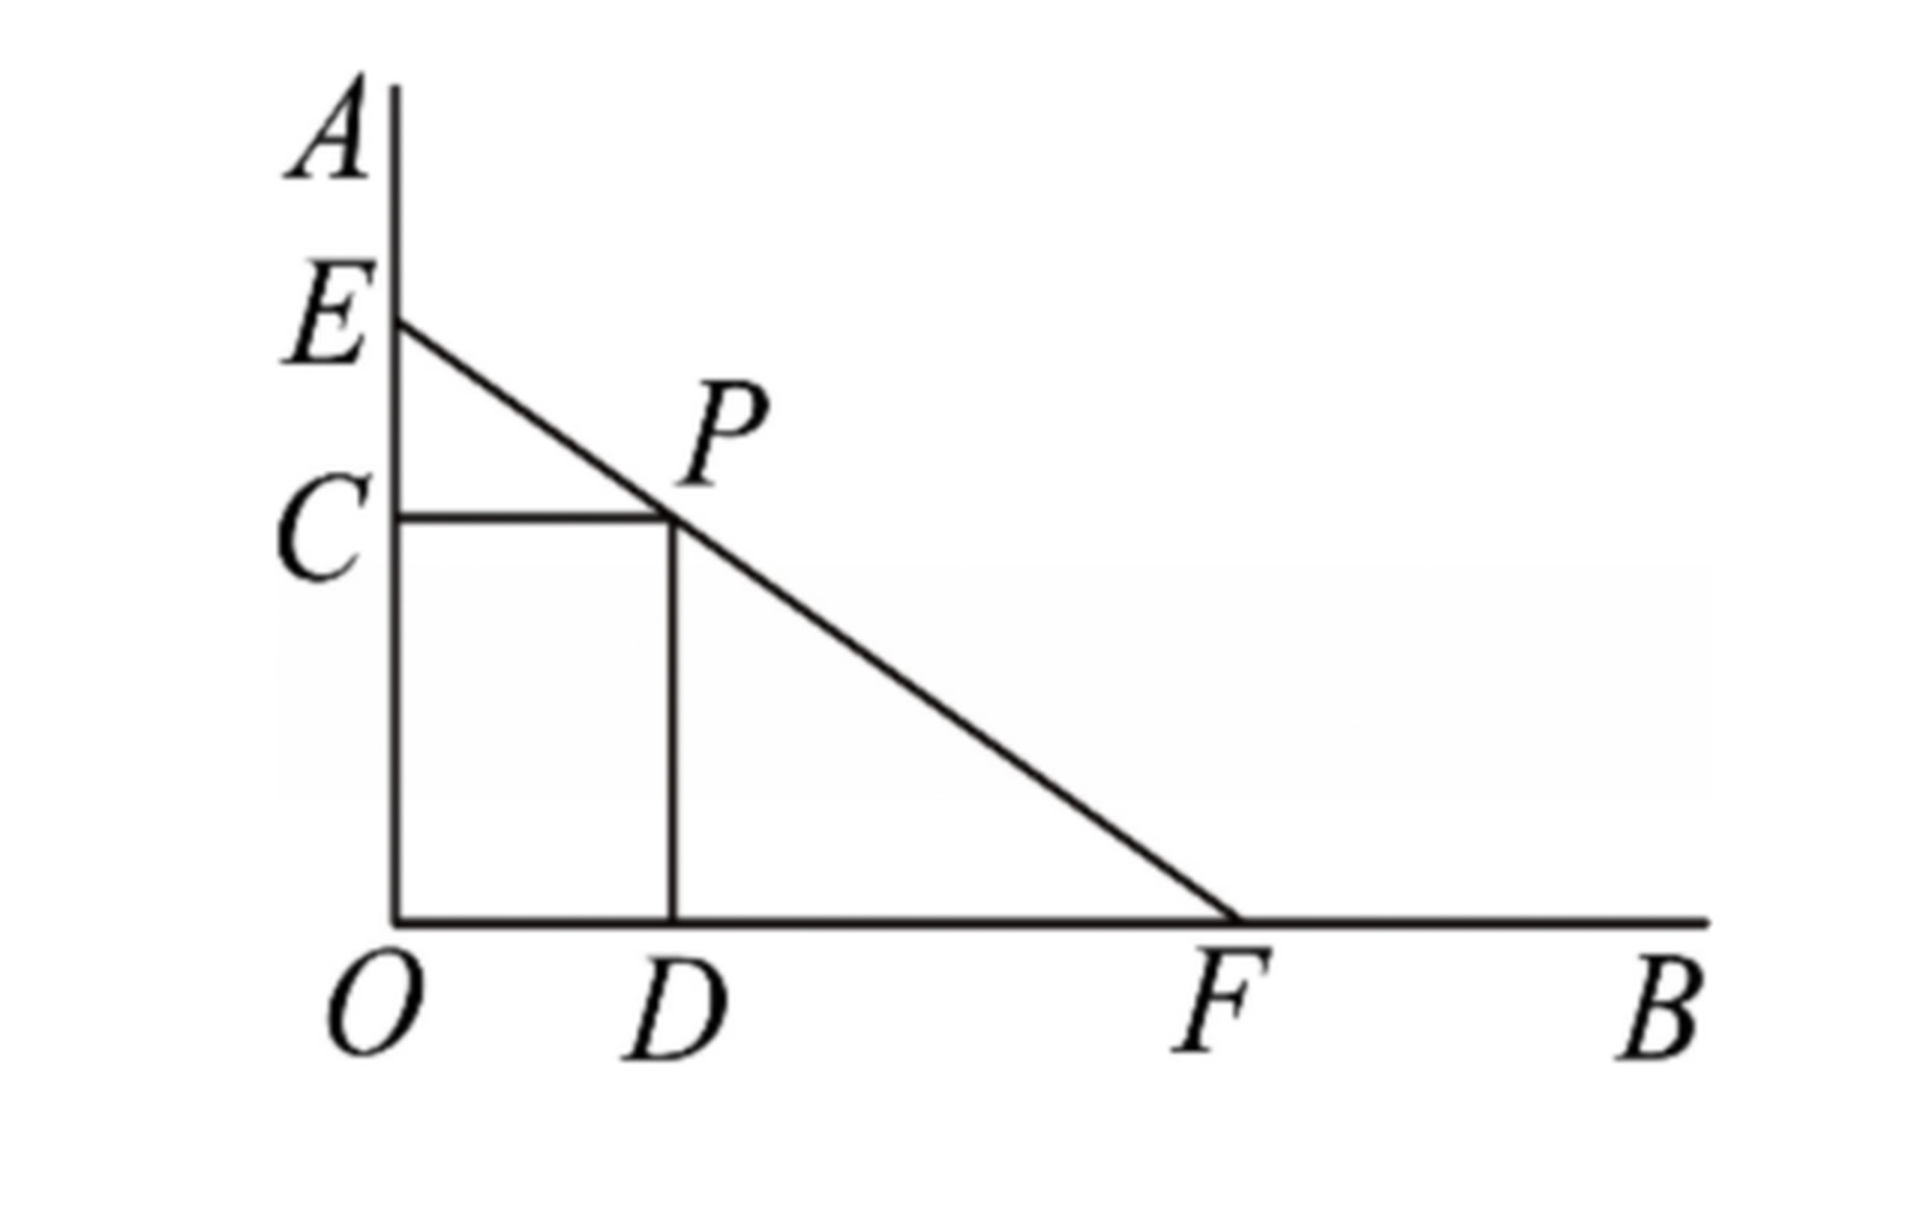
\includegraphics[width=0.32\textwidth]{figures/gao132_q18.png}
\end{center}

\ifanswer
\solbegin
\step{(1) 由题意得 $x\leq60$，}
\step{$\triangle PCE\sim\triangle FDP$，所以 $\dfrac{EC}{CP}=\dfrac{PD}{DF}$，即 $\dfrac{x}{25}=\dfrac{40}{DF}$，得 $DF=\dfrac{1000}{x}$m，}
\step{所以 $OF=OD+DF=\left(25+\dfrac{1000}x\right)$m，}
\step{所以 $25+\dfrac{1000}x\leq100$，解得 $x\geq\dfrac{40}3$；}
\step{综上，$\dfrac{40}3\leq x\leq60$；}
\step{(2) 由 $OE=OC+CE=(40+x)$m，}
\step{所以 $S=\dfrac12 OF\cdot OE=\dfrac12\left(25+\dfrac{1000}x\right)(40+x)$}
\step{$=\dfrac12\left(1000+25x+\dfrac{40000}x+1000\right)$m$^2$，}
\step{由基本不等式得 $S\geq\dfrac12\left(2000+2\sqrt{25x\cdot\dfrac{40000}x}\right)=2000$m$^2$，}
\step{当且仅当 $25x=\dfrac{40000}x$，即 $x=40$ 时取等号，}
\step{故 $EC=40$m 时，$S$ 取得最小值，为 $2000$m$^2$.}
\solend
\fi

\item 已知 $a>0$，$b>0$，请选择适当的方法证明.

(1) 若 $a\ne b$，证明：$a^3+b^3>a^2b+ab^2$；

(2) 若 $ab=1$，证明：$a^2+a<2$ 与 $b^2+b<2$ 不能同时成立.

\ifanswer
\solbegin
\step{(1) 因为 $a>0$，$b>0$，$a\ne b$，}
\step{所以 $a^3+b^3-a^2b-ab^2=a^2(a-b)+b^2(b-a)$}
\step{$=(a^2-b^2)(a-b)=(a-b)^2(a+b)>0$，所以 $a^3+b^3>a^2b+ab^2$.}
\step{(2) 假设 $a^2+a<2$ 与 $b^2+b<2$ 同时成立，所以 $-2<a<1,-2<b<1$，}
\step{又因为 $a>0,b>0$，所以 $0<a<1,0<b<1$，}
\step{所以 $0<ab<1$，这与 $ab=1$ 矛盾，}
\step{故 $a^2+a<2$ 与 $b^2+b<2$ 不可能同时成立.}
\solend
\fi

\item 若设 $M(a,n)=\lvert ax-1\rvert+\lvert ax-2\rvert+\cdots+\lvert ax-n\rvert$ 为曼哈顿扩张距离，它由 $n$ 个绝对值之和组成，其中 $n$ 为正整数.

(1) 若 $M(2,1)\leq5$，求 $x$ 的取值范围；

(2) 若 $k\leq M(2,2)$ 对一切实数 $x$ 恒成立，求实数 $k$ 的取值范围；

(3) $M(2,6)$ 是否存在最小值？若存在，求出该最小值与此时实数 $x$ 的取值范围；若不存在，说明理由.

\ifanswer
\solbegin
\step{(1) $M(2,1)=\lvert2x-1\rvert\leq5$，则不等式可化为 $-5\leq2x-1\leq5$，解得 $-2\leq x\leq3$，}
\step{所以 $x$ 的取值范围为 $[-2,3]$.}
\step{(2) 因为 $k\leq M(2,2)=\lvert2x-1\rvert+\lvert2x-2\rvert$ 对一切实数 $x$ 恒成立，}
\step{又 $\lvert2x-1\rvert+\lvert2x-2\rvert\geq\lvert(2x-1)-(2x-2)\rvert=1$，}
\step{当且仅当 $(2x-1)(2x-2)\leq0$，即 $\dfrac12\leq x\leq1$ 时取等号，}
\step{故 $k\leq1$，所以实数 $k$ 的取值范围为 $(-\infty,1]$.}
\step{(3) $M(2,6)=\lvert2x-1\rvert+\lvert2x-2\rvert+\lvert2x-3\rvert+\lvert2x-4\rvert+\lvert2x-5\rvert+\lvert2x-6\rvert$}
\step{$=2\left(\left\lvert x-\dfrac12\right\rvert+\lvert x-1\rvert+\left\lvert x-\dfrac32\right\rvert+\lvert x-2\rvert+\left\lvert x-\dfrac52\right\rvert+\lvert x-3\rvert\right)$，}
\step{其中 $\left\lvert x-\dfrac12\right\rvert+\lvert x-1\rvert+\left\lvert x-\dfrac32\right\rvert+\lvert x-2\rvert+\left\lvert x-\dfrac52\right\rvert+\lvert x-3\rvert$ 的几何意义为}
\step{在数轴上一点 $x$ 到 $\dfrac12,1,\dfrac32,2,\dfrac52,3$ 的距离之和，}
\step{要想距离之和最小，其中 $x\in\left[\dfrac12,3\right]$ 时，$\left\lvert x-\dfrac12\right\rvert+\lvert x-3\rvert$ 取得最小值，}
\step{当 $x\in\left[1,\dfrac52\right]$ 时，$\lvert x-1\rvert+\left\lvert x-\dfrac52\right\rvert$ 取得最小值，}
\step{当 $x\in\left[\dfrac32,2\right]$ 时，$\left\lvert x-\dfrac32\right\rvert+\lvert x-2\rvert$ 取得最小值，}
\step{综上，当 $x\in\left[\dfrac32,2\right]$ 时，$\left\lvert x-\dfrac12\right\rvert+\lvert x-1\rvert+\left\lvert x-\dfrac32\right\rvert+\lvert x-2\rvert+\left\lvert x-\dfrac52\right\rvert+\lvert x-3\rvert$}
\step{取得最小值，最小值为 $3-\dfrac12+\dfrac52-1+2-\dfrac32=\dfrac92$，}
\step{故 $M(2,6)=2\left(\left\lvert x-\dfrac12\right\rvert+\lvert x-1\rvert+\left\lvert x-\dfrac32\right\rvert+\lvert x-2\rvert+\left\lvert x-\dfrac52\right\rvert+\lvert x-3\rvert\right)$ 的}
\step{最小值为 $9$.}
\solend
\fi

\item 已知集合 $A=\{a_1,a_2,\cdots,a_n\}(0\leq a_1<a_2<\cdots<a_n,n\in\N,n\geq3)$ 具有性质 $Q$：对任意 $i,j(1\leq i\leq j\leq n)$，$a_i+a_j$ 与 $a_j-a_i$ 至少有一个属于集合 $A$；

(1) 判断集合 $M=\{0,2,4\}$ 与 $N=\{2,3,4\}$ 是否具有性质 $Q$，并说明理由；

(2) 已知 $A=\{a_1,a_2,a_3\}$ 具有性质 $Q$，当 $a_2=2026$ 时，求集合 $A$；

(3) 已知 $B=\{b_1,b_2,\cdots,b_{2026}\}$ 具有性质 $Q$，求 $\dfrac{b_1+b_2+\cdots+b_{2026}}{b_{2026}}$ 的值；

\ifanswer
\solbegin
\step{(1) 集合 $M=\{0,2,4\}$ 中，}
\step{因为 $0+2\in M,0+4\in M,4-2\in M,0\pm0=0\in M$，}
\step{$2+2=4\in M,2-2=0\in M,4-4=0\in M$，所以集合 $M$ 具有性质 $Q$；}
\step{集合 $N=\{2,3,4\}$ 中，因为 $3+3=6\notin N,3-3=0\notin N$，}
\step{所以集合 $N$ 不具有性质 $Q$.}
\step{(2) 因为 $a_1<a_2<a_3$，且 $A=\{a_1,a_2,a_3\}$ 具有性质 $Q$，}
\step{所以 $a_3+a_3\notin A,a_3-a_3=0\in A$，则 $a_1=0$，}
\step{又因为 $a_2+a_3>a_3$，所以 $a_2+a_3\notin A$，则 $a_3-a_2\in A$，}
\step{由集合的互异性得 $a_3-a_2=a_2$，而 $a_2=2026$，所以 $a_3=4052$，}
\step{故 $A=\{0,2026,4052\}$；}
\step{(3) 先证明一般结论：$A=\{a_1,a_2,\cdots,a_n\}(0\leq a_1<a_2<\cdots<a_n,n\in\N,n\geq3)$}
\step{具有性质 $Q$，则 $a_1+a_2+a_3+\cdots+a_n=\dfrac n2 a_n$.}
\step{因为 $A=\{a_1,a_2,\cdots,a_n\}(0\leq a_1<a_2<\cdots<a_n,n\in\N,n\geq3)$ 具有性质 $Q$，}
\step{所以 $a_n+a_n\notin A$，则 $a_n-a_n=0\in A$，则 $a_1=0$.}
\step{又因为 $0\leq a_1<a_2<\cdots<a_n$，所以 $0\leq a_n-a_n<a_n-a_{n-1}<\cdots<a_n-a_1$，}
\step{又因为 $a_n+a_{n-i}>a_n(i=1,2,\cdots,n-1)$，所以 $a_n+a_{n-i}\notin A$，}
\step{则 $a_n-a_{n-i}\in A$，}
\step{所以 $a_1=a_n-a_n,a_2=a_n-a_{n-1},a_3=a_n-a_{n-2},\cdots,a_n=a_n-a_1$.}
\step{所以 $a_1+a_2+a_3+\cdots+a_n$}
\step{$=(a_n-a_n)+(a_n-a_{n-1})+(a_n-a_{n-2})+\cdots+(a_n-a_1)$，}
\step{即 $a_1+a_2+a_3+\cdots+a_n=\dfrac n2 a_n$，}
\step{所以 $B=\{b_1,b_2,\cdots,b_{2026}\}$ 具有性质 $Q$，则 $b_1+b_2+\cdots+b_{2026}=\dfrac{2026}{2}b_{2026}$，}
\step{所以 $\dfrac{b_1+b_2+\cdots+b_{2026}}{b_{2026}}=\dfrac{2026}{2}=1013$.}
\solend
\fi

\end{enumerate}

% 行数复核：逐题数 \step 条数，合计 144 条（Q3：4；Q4：1；Q5：4；Q6：2；Q7：9；Q8：2；
% Q9：3；Q10：6；Q11：9；Q12：9；Q13：0；Q14：9；Q15：4；Q16：19；Q17：5；Q18：11；
% Q19：7；Q20：17；Q21：23），与原卷印刷行逐题相等（cases 块作一个印刷行计）。
% 第 13 题只印括号内答案、提 \ans{}，不计入 \step 账；第 14—16 题答案在解析末句，
% 括号内留空、不另提 \ans{}。

\end{document}
"
% 紧凑版：xelatex "\def\iscompact{1}% 高一132_川沙中学_期中.tex
%   —— 高一上数学"2026-2027 年川沙中学高一上期中"（试卷版/答案版）
% 试卷版：xelatex 高一132_川沙中学_期中.tex
% 答案版：xelatex "\def\isanswer{1}% 高一132_川沙中学_期中.tex
%   —— 高一上数学"2026-2027 年川沙中学高一上期中"（试卷版/答案版）
% 试卷版：xelatex 高一132_川沙中学_期中.tex
% 答案版：xelatex "\def\isanswer{1}\input{高一132_川沙中学_期中.tex}"
% 紧凑版：xelatex "\def\iscompact{1}\input{高一132_川沙中学_期中.tex}"
%
% 原始材料：微信公众号"魔都数学加油站"文章，作者破晓，2026-11-14 19:00 发布；
% 连载"27学年高一132"，原文标题"27学年高一132——2026-2027年上海市川沙中学高一上期中"；
% 原文链接：https://mp.weixin.qq.com/s/VBG01CrUNMIYWWHhSfz8JQ。
% 正文为 11 张 PNG 页（01、04、06、07、09、11 为 2560x3620，02、03、05、08、10 为 4762x6735），
% 题目下印有【解析】，为讲评版。题目、解析均据原图转录；
% 卷面粉红色水印"魔都数学加油站"及公众号页脚未录入。全卷 2 幅插图：第 14 题四幅坐标图选项、
% 第 18 题矩形 OCPD 与小路 EF 示意图，均取原卷 04／07 页截图去水印。
%
% 卷首标题：原卷印作"2026-2027 年川沙中学高一上期中"（公众号标题中的"上海市"
% 卷面标题行没有，本稿照卷面），年份区间按全稿惯例排 en dash；原卷未印副标题，
% 本卷为期中卷、跨集合与常用逻辑用语／不等式／函数三章，按题目内容标为
% "集合与常用逻辑用语、不等式、函数"（与 125／126／128／129／131 同期中卷口径相同）：
% 集合与逻辑见 Q5、Q6、Q17、Q21，不等式见 Q3、Q4、Q9、Q10、Q12、Q13、Q15、Q16、Q19，
% 函数（幂函数、指数／对数、基本不等式应用）见 Q7、Q8、Q11、Q14、Q18、Q20。
%
% 题号体例：本卷共 19 题——一、填空题 3—12（10 题）、二、选择题 13—16（4 题）、
% 三、解答题 17—21（5 题）。三节分别 \setcounter{enumi}{2}／{12}／{16}。
%
% 与原卷的排版差异：
%   ① 原文从第 3 题起，本稿保留原题号（见上"题号体例"）；
%   ② 原卷每题下直接印【解析】，本稿按全稿惯例置于答案版；第 13 题答案 D 印在题干
%      括号内、无独立答案段，按 高一37／52／53／55／63／64／128／131 成例括号留空、
%      另提 \ans{$D$}；第 14—16 题答案在解析末句"故选 …"，括号内留空、不另提 \ans{}；
%   ③ 原卷未印副标题，本稿按"知识模块"口径补出；
%   ④ 原卷填空横线按全稿惯例排为 \blankline[4.4em]；选择题括号排 \mbox{（\quad）}、
%      选项段前按惯例加 \keepwithprev；解答题不留作答区（原卷为讲评版，与 109—131 同）；
%   ⑤ 原卷数集排斜体 $R^+$／$R$／$Z$／$N$，按全稿惯例改 \R^+／\R／\Z／\N；
%      绝对值排 \lvert…\rvert，集合描述竖线排 \mid；不等号按全稿惯例排 \leqslant／\geqslant；
%      补集照原卷上划线排 \overline{B}；
%   ⑥ 子题标号 (1)(2)(3) 原卷用半角括号，照录；第 14 题四幅坐标图选项按原卷 2×2 排布
%      合并裁为一张 \includegraphics（未用 TikZ 重绘，以保证与原卷一致），题前加
%      \needvspace{9cm} 守卫；第 18 题图取 07 页截图，题前按惯例加 \needvspace{7cm} 守卫
%      （照 高一120／127／129／131 成例），两者守卫都放在 \item 之前；
%   ⑦ 原卷 Q7 解析跨 01—02 页、Q10 解析跨 02—03 页、Q12 解析跨 03—04 页、
%      Q14 解析跨 04—05 页、Q16 解析在 06 页、Q18 解析跨 07—08 页、
%      Q20 解析跨 08—09 页、Q21 解析跨 10—11 页，本稿按题合并连续排版；
%      末页第 11 页为 Q21 (3) 解析的续尾，按实际印刷行单列。
%
% 判别式字形：第 10 题 $\triangle=4(a-1)^2+16(a-1)<0$、第 11 题
%   $\triangle=4(m-2)^2-4(m^2-3m+3)=-4m+4>0$ 两处原卷均排 $\triangle$（等边、扁），
%   逐处放大核对、字形一致，照录 \triangle；与 高一129／131 同题排 $\Delta$（等腰、高）不同。
%   全卷 \triangle 兼作第 18 题「$\triangle PCE\sim\triangle FDP$」「$\triangle OEF$」的几何
%   三角形记号，全卷未出现 \Delta。
%
% 子集符号：第 5 题解析 $B\subseteq A$、第 17 题 (2) 解析 $A\subseteq B$ 均印带下划线，
%   照录 \subseteq；全卷未出现单线 \subset。
%
% 原卷存疑照录：
%   第 9 题题干作"充分非必要条件"、解析作"充分不必要条件"，措辞不同，照录；
%   第 10 题解析"当 $a-1=0$ 时，$-4\geq0$，不等式不成立，$a=1$ 满足题意"照录；
%   第 11 题解析"所以 $2(m-1)+\dfrac1{m-1}\leq-2\sqrt2$"由上一行 $2(1-m)+\dfrac1{1-m}\geq2\sqrt2$
%     直接变号得到，照录；
%   第 12 题解析"由 $x\in Z$，$-7<-2\sqrt{10}<-6$"与"即 $k^2+7k+10\leq0$，解得 $-5\leq k\leq-2$"照录；
%   第 16 题解析"令 $52\times(930+a)=-52$，解得 $a=-931$"（按式应为 $a=-931$ 之外的解）照录；
%   第 19 题 (2) 解析"所以 $-2<a<1,-2<b<1$"数学式内半角逗号，照录；
%   第 20 题 (3) 解析"最小值为 $3-\dfrac12+\dfrac52-1+2-\dfrac32=\dfrac92$"与
%     "故 $M(2,6)=\dots$ 的最小值为 9"两处结论并列，照录；
%   第 21 题 (1) 解析"$0+2\in M,0+4\in M,4-2\in M,0\pm0=0\in M$"、
%     "$2+2=4\in M,2-2=0\in M,4-4=0\in M$"、(3) 各连写等式内半角逗号，照录；
%   第 21 题 (3) 解析"即 $a_1+a_2+a_3+\cdots+a_n=\dfrac n2 a_n$，"句末用半角逗号，照录。
%
% 行数复核：见文末"行数复核"注（逐题 \step 条数与原卷印刷行逐题相等，cases 块作一个印刷行计）。
%   第 13 题只印括号内答案、提 \ans{}，不计入 \step 账；第 14—16 题答案在解析末句，
%   括号内留空、不另提 \ans{}。
%
\documentclass[a4paper,11pt]{article}
\usepackage{common}

\begin{document}

\examtitlest[3]{2026--2027 年川沙中学高一上期中}{集合与常用逻辑用语、不等式、函数}

\bigsec{一、填空题}

\begin{enumerate}
\setcounter{enumi}{2}

\item 已知 $a$、$b\in\R^+$ 且 $ab=2$，则 $a+2b$ 的最小值为\blankline[4.4em].

\ifanswer
\solbegin
\step{因为 $a\in\R^+$，$b\in\R^+$ 且 $ab=2$，}
\step{由基本不等式得 $a+2b\geq2\sqrt{a\cdot2b}=2\sqrt{2ab}=2\sqrt4=4$.}
\step{等号当且仅当 $a=2b$ 时成立，结合 $ab=2$ 解得 $b=1$，$a=2$，}
\step{所以 $a+2b$ 的最小值为 $4$.}
\solend
\fi

\item 如果幂函数 $f(x)=(m^2-3m-3)x^{m^2+m-3}$ 在 $(0,+\infty)$ 上是增函数，则实数 $m=$\blankline[4.4em].

\ifanswer
\solbegin
\step{由已知得 $\begin{cases}m^2-3m-3=1\\m^2+m-3>0\end{cases}$，所以 $m=4$.}
\solend
\fi

\item 已知集合 $A=\{1,2\}$，集合 $B=\{x\mid ax=6\}$，若 $A\cup B=A$，则 $a$ 的所有取值构成的集合为\blankline[4.4em].

\ifanswer
\solbegin
\step{因为 $A\cup B=A$，所以 $B\subseteq A$，}
\step{当 $a=0$ 时，$B=\varnothing$，满足 $B\subseteq A$；}
\step{当 $a\ne0$ 时，$B=\left\{\dfrac6a\right\}$，则 $\dfrac6a=1$ 或 $\dfrac6a=2$，解得 $a=6$ 或 $a=3$，}
\step{综上所述，$a$ 的所有取值构成的集合为 $\{0,3,6\}$.}
\solend
\fi

\item 设全集为 $\R$，$A=\{y\mid y=-x^2+2x+1\}$，$B=\{x\mid y=\ln(x-1)\}$，则 $A\cap B=$\blankline[4.4em].

\ifanswer
\solbegin
\step{$A=\{y\mid y=-x^2+2x+1\}=\{y\mid y=-(x-1)^2+2\}=\{y\mid y\leq2\}$，}
\step{$B=\{x\mid y=\ln(x-1)\}=\{x\mid x>1\}$，则 $A\cap B=(1,2]$.}
\solend
\fi

\item 已知 $x\in\R$，则方程 $\lvert 6-x\rvert+\lvert 6x-3\rvert=\lvert 5x+3\rvert$ 的解集为\blankline[4.4em].

\ifanswer
\solbegin
\step{当 $x<-\dfrac35$ 时，$6-x>0$，$6x-3<0$，$5x+3<0$，}
\step{原方程为 $6-x-6x+3=-5x-3$，解得 $x=6$，不满足 $x<-\dfrac35$；}
\step{当 $-\dfrac35\leq x\leq\dfrac12$ 时，$5x+3\geq0$，$6x-3<0$，$6-x>0$，}
\step{原方程为 $6-x+3-6x=5x+3$，解得 $x=\dfrac12$；}
\step{当 $\dfrac12<x\leq6$ 时，$5x+3>0$，$6x-3>0$，$6-x\geq0$，}
\step{原方程为 $6-x+6x-3=5x+3$，即 $0=0$，恒成立，所以 $\dfrac12<x\leq6$；}
\step{当 $x>6$ 时，$5x+3\geq0$，$6x-3>0$，$6-x<0$，}
\step{原方程为 $x-6+6x-3=5x+3$，解得 $x=6$，不满足 $x>6$；}
\step{综上 $\dfrac12\leq x\leq6$，所以原方程的解集为 $\left\{x\mid\dfrac12\leq x\leq6\right\}$.}
\solend
\fi

\item 已知 $\log_2 3=a,2^b=7$，用 $a,b$ 表示 $\log_{42}56$ 为\blankline[4.4em].

\ifanswer
\solbegin
\step{$\log_{42}56=\dfrac{\log_2 56}{\log_2 42}=\dfrac{\log_2(7\times8)}{\log_2(6\times7)}=\dfrac{\log_2 7+\log_2 8}{\log_2 6+\log_2 7}$}
\step{$=\dfrac{\log_2 7+\log_2 2^3}{\log_2 2+\log_2 3+\log_2 7}=\dfrac{b+3}{1+a+b}$.}
\solend
\fi

\item 已知 $\dfrac13<x<\dfrac12$ 是不等式 $\lvert x-m\rvert<1$ 成立的充分非必要条件，则 $m$ 的取值范围是\blankline[4.4em].

\ifanswer
\solbegin
\step{因为 $\lvert x-m\rvert<1$，所以 $-1<x-m<1$，所以 $m-1<x<m+1$，}
\step{所以 $m-1<x<m+1$ 成立的充分不必要条件是 $\dfrac13<x<\dfrac12$，}
\step{所以 $\begin{cases}m-1\leq\dfrac13\\m+1\geq\dfrac12\end{cases}$，解得 $-\dfrac12\leq m\leq\dfrac43$，故 $m$ 的取值范围是 $\left[-\dfrac12,\dfrac43\right]$.}
\solend
\fi

\item 若关于 $x$ 的不等式 $(a-1)x^2+2(a-1)x-4\geq0$ 的解集为空集，则 $a$ 的取值范围是\blankline[4.4em].

\ifanswer
\solbegin
\step{关于 $x$ 的不等式 $(a-1)x^2+2(a-1)x-4\geq0$ 的解集为 $\varnothing$，}
\step{当 $a-1=0$ 时，$-4\geq0$，不等式不成立，$a=1$ 满足题意；}
\step{当 $a-1>0$ 时，$a>1$，不等式的解集不为空集，不满足题意；}
\step{当 $a-1<0$ 时，$a<1$，当 $\triangle=4(a-1)^2+16(a-1)<0$ 时，即 $(a-1)(a+3)<0$，}
\step{解得 $-3<a<1$，满足题意；}
\step{综上，实数 $a$ 的取值范围是 $\{a\mid-3<a\leq1\}$.}
\solend
\fi

\item 已知关于 $x$ 的方程 $x^2+2(m-2)x+m^2-3m+3=0$ 有两个不相等的实数根 $x_1$、$x_2$，则 $\dfrac{mx_1}{x_1-1}+\dfrac{mx_2}{x_2-1}-\dfrac{2}{x_1+x_2-2}$ 的最大值为\blankline[4.4em].

\ifanswer
\solbegin
\step{关于 $x$ 的方程 $x^2+2(m-2)x+m^2-3m+3=0$ 有两个不相等的实数根 $x_1$、$x_2$，}
\step{则 $\triangle=4(m-2)^2-4(m^2-3m+3)=-4m+4>0$，得 $m<1$，}
\step{且 $x_1+x_2=-2(m-2)$，$x_1x_2=m^2-3m+3$，}
\step{$\dfrac{mx_1}{x_1-1}+\dfrac{mx_2}{x_2-1}-\dfrac{2}{x_1+x_2-2}=\dfrac{m[2x_1x_2-(x_1+x_2)]}{x_1x_2-(x_1+x_2)+1}+\dfrac1{m-1}$}
\step{$=\dfrac{2m(m-1)^2}{m^2-m}+\dfrac1{m-1}=2(m-1)+\dfrac1{m-1}$，}
\step{又因为 $m<1$，所以 $m-1<0$，则 $1-m>0$，}
\step{所以 $2(1-m)+\dfrac1{1-m}\geq2\sqrt{2(1-m)\cdot\dfrac1{1-m}}=2\sqrt2$，}
\step{当且仅当 $2(1-m)=\dfrac1{1-m}$ 时，即 $m=1-\dfrac{\sqrt2}2$ 时取等号，}
\step{所以 $2(m-1)+\dfrac1{m-1}\leq-2\sqrt2$，即 $\dfrac{mx_1}{x_1-1}+\dfrac{mx_2}{x_2-1}-\dfrac2{x_1+x_2-2}$ 的最大值为 $-2\sqrt2$.}
\solend
\fi

\item 若使集合 $A=\{x\mid(kx-k^2-10)(x-1)>0,x\in\Z\}$ 中的元素个数最少，则实数 $k$ 的取值范围是\blankline[4.4em].

\ifanswer
\solbegin
\step{由题意集合 $A=\{x\mid(kx-k^2-10)(x-1)>0,\ x\in\Z\}$，}
\step{$k=0$ 时，不等式解得 $x<1$，有无数个整数解；}
\step{$k\ne0$ 时，则不等式变形为 $k\left(x-k-\dfrac{10}k\right)(x-1)>0$，}
\step{当 $k>0$ 时，$k+\dfrac{10}k\geq2\sqrt{10}$，仅当 $k=\sqrt{10}$ 时等号成立，}
\step{此时不等式解得 $x>k+\dfrac{10}k$ 或 $x<1$，有无数个整数解；}
\step{当 $k<0$ 时，$k+\dfrac{10}k=-\left[(-k)+\left(-\dfrac{10}k\right)\right]\leq-2\sqrt{10}$，仅当 $k=-\sqrt{10}$ 时等号成立，}
\step{此时不等式解得 $k+\dfrac{10}k<x<1$，}
\step{由 $x\in\Z$，$-7<-2\sqrt{10}<-6$，要使集合 $A$ 中的元素最少，则 $k+\dfrac{10}k\geq-7$，}
\step{即 $k^2+7k+10\leq0$，解得 $-5\leq k\leq-2$，故实数 $k$ 的取值范围是 $[-5,-2]$.}
\solend
\fi

\end{enumerate}

\bigsec{二、选择题}

\begin{enumerate}
\setcounter{enumi}{12}

\item 下列说法正确的是\mbox{（\quad）}

\keepwithprev
A. 若 $a>b$，则 $\dfrac1a<\dfrac1b$\qquad\qquad B. 若 $a>b$，$c>d$，则 $ac>bd$

C. 若 $a>b$，则 $ac^2>bc^2$\qquad\qquad D. 若 $ac^2>bc^2$，则 $a>b$

\ifanswer
\ans{$D$}
\fi

% 第 14 题四幅坐标图选项是一整块，守卫放在 \item 之前
\needvspace{9cm}
\item 在同一坐标系内，函数 $y=x^a(a\ne0)$ 和 $y=ax-\dfrac1a$ 的图象可能是\mbox{（\quad）}

\keepwithprev
\begin{center}
% 四幅坐标图选项取原卷 04 页截图去粉色水印，按原卷 2×2 排布合并为一张
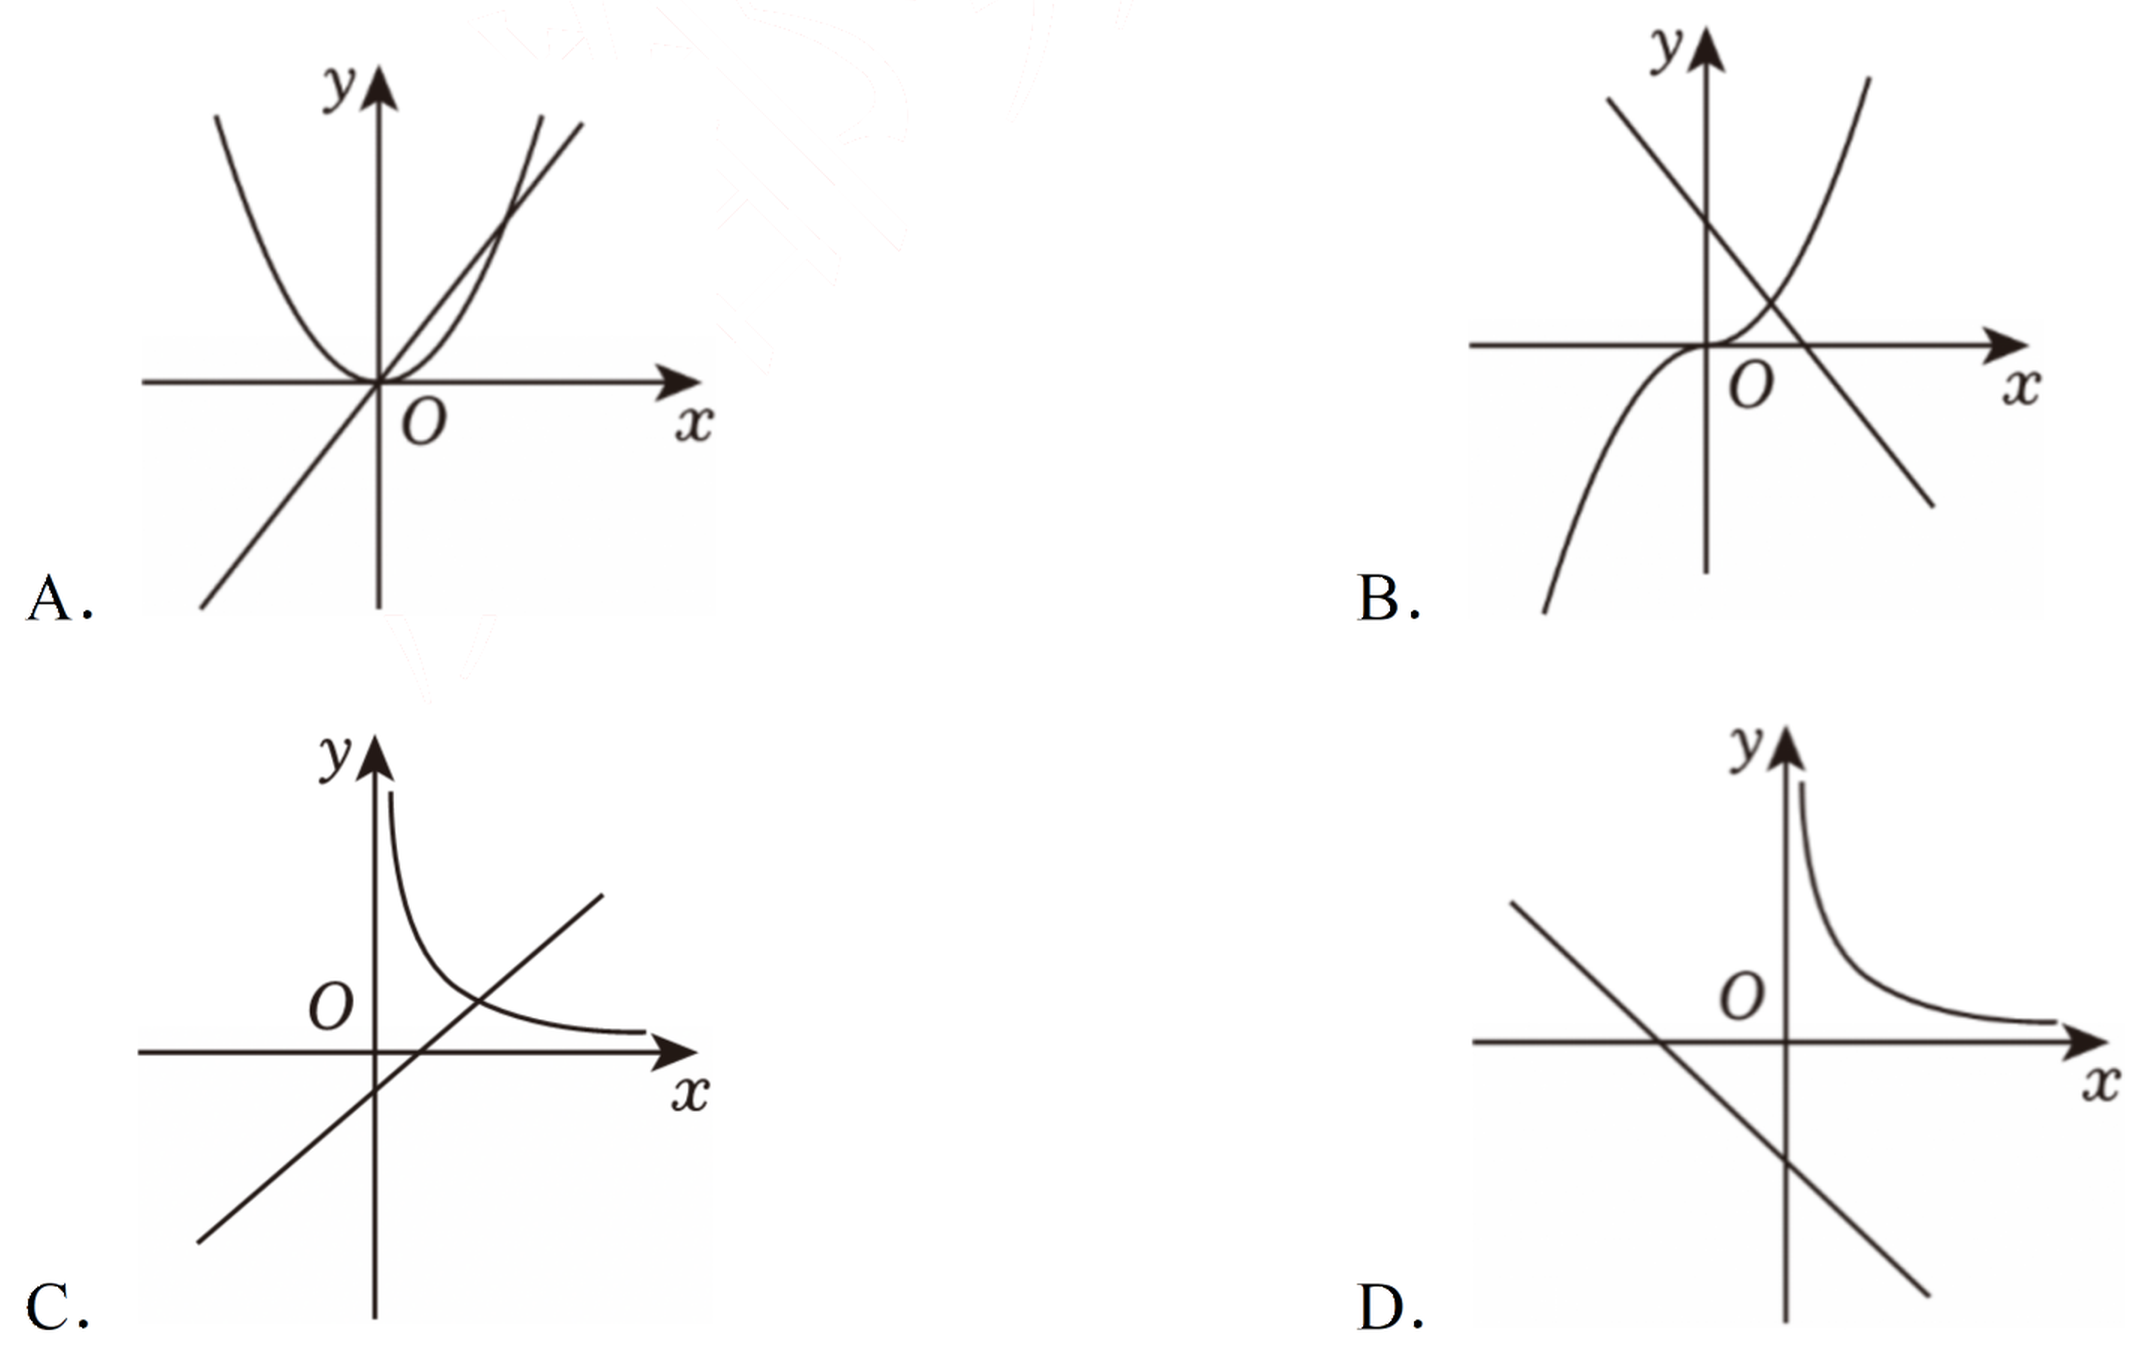
\includegraphics[width=0.80\textwidth]{figures/gao132_q14.png}
\end{center}

\ifanswer
\solbegin
\step{当 $a>0$ 时，$y=ax-\dfrac1a$ 严格增，当 $a<0$ 时，$y=ax-\dfrac1a$ 严格减，}
\step{对于 $A$，因为 $a\ne0$，所以直线 $y=ax-\dfrac1a$ 不过原点，故 $A$ 错误；}
\step{对于 $B$，由函数 $y=x^a(a\ne0)$ 的图象得 $a>1$，}
\step{由 $y=ax-\dfrac1a$ 的图象得 $a<0$，互相矛盾，故 $B$ 错误；}
\step{对于 $C$，由函数 $y=x^a(a\ne0)$ 的图象得 $a>1$，}
\step{由 $y=ax-\dfrac1a$ 的图象得 $a>0$ 且 $-\dfrac1a<0$，符合题意，故 $C$ 正确；}
\step{对于 $D$，由函数 $y=x^a(a\ne0)$ 的图象得 $a<0$，}
\step{由 $y=ax-\dfrac1a$ 的图象得 $a<0$ 且 $-\dfrac1a<0$，互相矛盾，故 $D$ 错误；}
\step{故选 $C$.}
\solend
\fi

\item 中国的 $5G$ 技术领先世界，在 $5G$ 技术中，最大数据传输速率 $C$ 取决于信道带宽 $W$，$C$ 与 $W$ 满足 $C=W\log_2\left(1+\dfrac SN\right)$，其中 $\dfrac SN$ 称为信噪比（单位：$dB$）. 若不改变带宽 $W$，初始信噪比 $\dfrac SN$ 为 $1000$，那么为了使 $C$ 增加 $30\%$，需要将信噪比 $\dfrac SN$ 从 $1000$ 提升至大约\mbox{（\quad）}

\keepwithprev
A. $5000$\qquad\qquad B. $6000$\qquad\qquad C. $7000$\qquad\qquad D. $8000$

\ifanswer
\solbegin
\step{由题意得 $\dfrac SN=1000$ 时，$C=W\log_2(1+1000)\approx W\log_2 1000$，}
\step{要使 $C$ 增加 $30\%$，则 $(1+30\%)C=W\log_2\left(1+\dfrac SN\right)$，即 $1.3C\approx W\log_2\dfrac SN$，}
\step{所以 $1.3\approx\log_{1000}\dfrac SN=\dfrac{\lg\frac SN}{\lg1000}$，所以 $\lg\dfrac SN=3.9$，所以 $\dfrac SN=10^{3.9}\approx8000$.}
\step{故选 $D$.}
\solend
\fi

\item 对于 $a\in\R$，设非空集合 $A=\left\{x\mid\dfrac{(x^2-930x+a)(x-52)}{x+a}=0\right\}$，记 $A$ 中的所有元素之和为 $S(a)$，所有元素之积为 $T(a)$，则下列说法中，不正确的是\mbox{（\quad）}

\keepwithprev
A. 存在实数 $a$，使得 $S(a)=930$

B. 存在实数 $a$，使得 $T(a)=517$

C. 不存在实数 $a$，使得 $T(a)=0$

D. 恰存在 $1$ 个实数 $a$，使得 $T(a)=-52$

\ifanswer
\solbegin
\step{由分式值为 $0$，得分子为 $0$ 且分母不为 $0$，}
\step{分子 $(x^2-930x+a)(x-52)=0$ 的根为 $x=52$}
\step{及方程 $x^2-930x+a=0$ 的两根 $x_1$，$x_2$，}
\step{由根与系数的关系得 $x_1+x_2=930$，$x_1\cdot x_2=a$，}
\step{分母限制 $x\ne-a$，需要剔除等于 $-a$ 的根，}
\step{选项 $A$，取 $a=-52$，$x=52$ 为增根舍去，集合 $A=\{x_1,x_2\}$，}
\step{元素之和 $S(a)=930$，故 $A$ 正确；}
\step{选项 $B$，当无增根时，$T(a)=52a$，令 $52a=517$，得 $a=\dfrac{517}{52}$，}
\step{验证无增根，存在这样的 $a$，故 $B$ 正确；}
\step{选项 $C$，若 $T(a)=0$，则 $0\in A$，代入分子得 $a=0$，}
\step{但 $a=0$ 时分母 $x\ne0$，$x=0$ 为增根，$0$ 不能属于集合 $A$，}
\step{故不存在 $a$ 使得 $T(a)=0$，故 $C$ 正确；}
\step{选项 $D$，当无增根时，令 $52a=-52$，得 $a=-1$；}
\step{当 $x=-a$ 是二次方程的根且不等于 $52$ 时，}
\step{令 $52\times(930+a)=-52$，解得 $a=-931$，验证符合条件；}
\step{当 $a=-52$ 时，$x=52$，舍去，}
\step{集合 $A=\{x_1,x_2\}$，$T(a)=a=-52$，得到两个满足条件的 $a$；}
\step{因此存在 $3$ 个满足条件的 $a$，故 $D$ 错误.}
\step{故选 $D$.}
\solend
\fi

\end{enumerate}

\bigsec{三、解答题}

\begin{enumerate}
\setcounter{enumi}{16}

\item 已知全集 $U=\R$，集合 $A=\left\{x\mid\dfrac{x}{x-3}<0\right\}$，$B=\{x\mid(x-a)(x+4-a)<0\}$.

(1) 当 $a=2$ 时，求 $\overline{B}$、$A\cap\overline{B}$；

(2) 若 $A\cap B=A$，求实数 $a$ 的取值范围.

\ifanswer
\solbegin
\step{(1) $\dfrac{x}{x-3}<0$，即 $x(x-3)<0$，解得 $A=\{x\mid0<x<3\}$，}
\step{当 $a=2$ 时，$B=\{x\mid(x-a)(x+4-a)<0\}=\{x\mid-2<x<2\}$，}
\step{则 $\overline{B}=\{x\mid x\leq-2$ 或 $x\geq2\}$，故 $A\cap\overline{B}=\{x\mid2\leq x<3\}$；}
\step{(2) $A\cap B=A$，则 $A\subseteq B$，故 $\begin{cases}a-4\leq0\\a\geq3\end{cases}$，解得 $3\leq a\leq4$，}
\step{故实数 $a$ 的取值范围是 $\{a\mid3\leq a\leq4\}$.}
\solend
\fi

% 第 18 题是"题干 + 图"约 7cm 的一整块，守卫放在 \item 之前
\needvspace{7cm}
\item 如图，$OA$、$OB$ 是两条长度足够长的互相垂直的笔直小路，矩形 $OCPD$ 的顶点 $C$、$D$ 分别在 $OA$、$OB$ 上，且该矩形区域内种满了荷花. 为了让观赏者有更好的观赏体验，现计划经过点 $P$ 修一条小路 $EF$，其中点 $E$ 在小路 $OA$ 上，点 $F$ 在小路 $OB$ 上，并在 $\triangle OEF$ 区域内种满荷花. 已知 $OD=25m$，$OC=40m$，且小路 $EF$ 要完全位于一个以 $O$ 为顶点的，边长为 $100$ m 的正方形内部（包括边界）. 记 $\triangle OEF$ 的面积为 $S$m$^2$.

(1) 设 $EC=x\cdot m$，试用 $x$ 表示 $OF$，并求 $x$ 的取值范围.

(2) 当 $EC$ 的长度为多少时，$S$ 取得最小值？最小值是多少？

\begin{center}
% 图取原卷 07 页截图去粉色水印，3× LANCZOS 放大
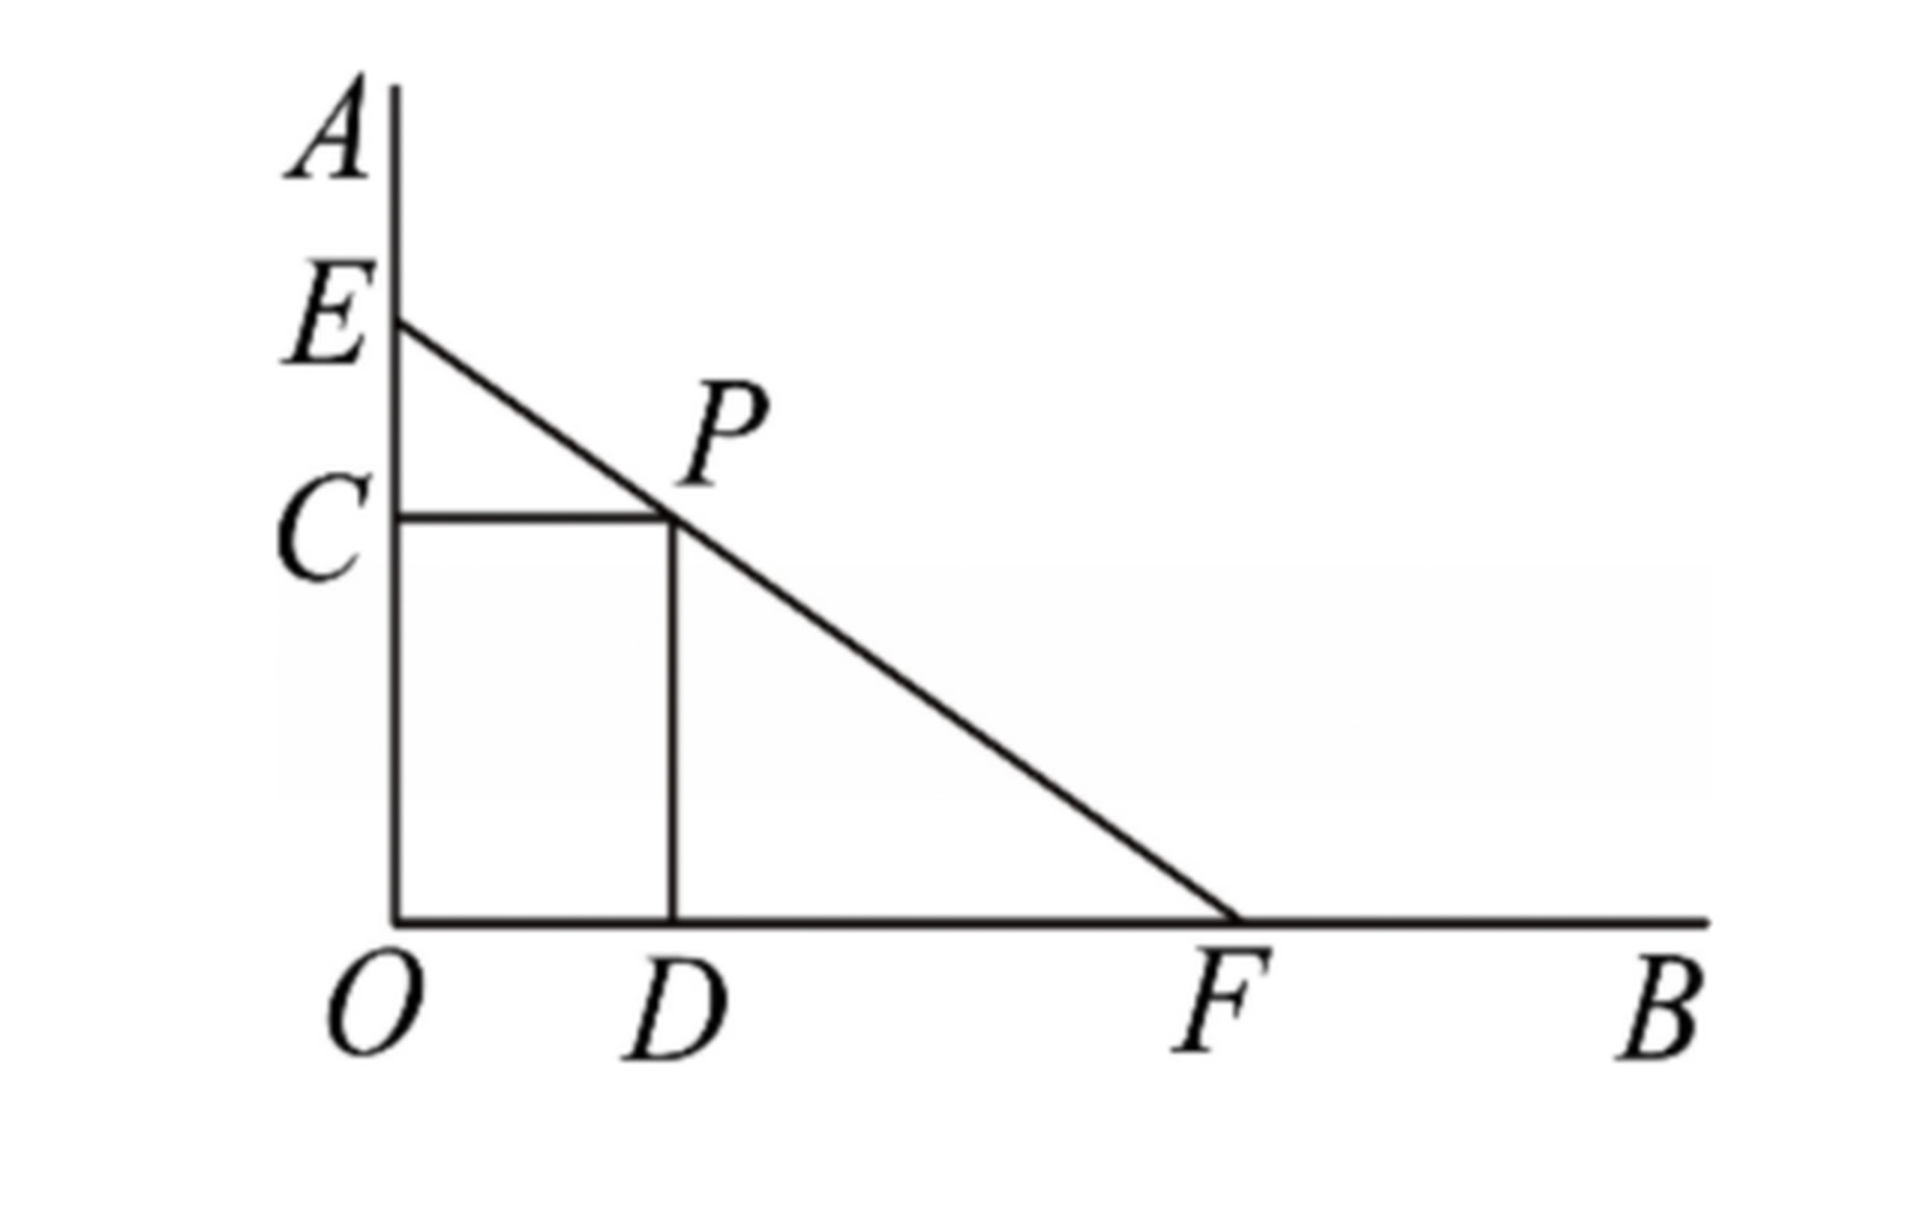
\includegraphics[width=0.32\textwidth]{figures/gao132_q18.png}
\end{center}

\ifanswer
\solbegin
\step{(1) 由题意得 $x\leq60$，}
\step{$\triangle PCE\sim\triangle FDP$，所以 $\dfrac{EC}{CP}=\dfrac{PD}{DF}$，即 $\dfrac{x}{25}=\dfrac{40}{DF}$，得 $DF=\dfrac{1000}{x}$m，}
\step{所以 $OF=OD+DF=\left(25+\dfrac{1000}x\right)$m，}
\step{所以 $25+\dfrac{1000}x\leq100$，解得 $x\geq\dfrac{40}3$；}
\step{综上，$\dfrac{40}3\leq x\leq60$；}
\step{(2) 由 $OE=OC+CE=(40+x)$m，}
\step{所以 $S=\dfrac12 OF\cdot OE=\dfrac12\left(25+\dfrac{1000}x\right)(40+x)$}
\step{$=\dfrac12\left(1000+25x+\dfrac{40000}x+1000\right)$m$^2$，}
\step{由基本不等式得 $S\geq\dfrac12\left(2000+2\sqrt{25x\cdot\dfrac{40000}x}\right)=2000$m$^2$，}
\step{当且仅当 $25x=\dfrac{40000}x$，即 $x=40$ 时取等号，}
\step{故 $EC=40$m 时，$S$ 取得最小值，为 $2000$m$^2$.}
\solend
\fi

\item 已知 $a>0$，$b>0$，请选择适当的方法证明.

(1) 若 $a\ne b$，证明：$a^3+b^3>a^2b+ab^2$；

(2) 若 $ab=1$，证明：$a^2+a<2$ 与 $b^2+b<2$ 不能同时成立.

\ifanswer
\solbegin
\step{(1) 因为 $a>0$，$b>0$，$a\ne b$，}
\step{所以 $a^3+b^3-a^2b-ab^2=a^2(a-b)+b^2(b-a)$}
\step{$=(a^2-b^2)(a-b)=(a-b)^2(a+b)>0$，所以 $a^3+b^3>a^2b+ab^2$.}
\step{(2) 假设 $a^2+a<2$ 与 $b^2+b<2$ 同时成立，所以 $-2<a<1,-2<b<1$，}
\step{又因为 $a>0,b>0$，所以 $0<a<1,0<b<1$，}
\step{所以 $0<ab<1$，这与 $ab=1$ 矛盾，}
\step{故 $a^2+a<2$ 与 $b^2+b<2$ 不可能同时成立.}
\solend
\fi

\item 若设 $M(a,n)=\lvert ax-1\rvert+\lvert ax-2\rvert+\cdots+\lvert ax-n\rvert$ 为曼哈顿扩张距离，它由 $n$ 个绝对值之和组成，其中 $n$ 为正整数.

(1) 若 $M(2,1)\leq5$，求 $x$ 的取值范围；

(2) 若 $k\leq M(2,2)$ 对一切实数 $x$ 恒成立，求实数 $k$ 的取值范围；

(3) $M(2,6)$ 是否存在最小值？若存在，求出该最小值与此时实数 $x$ 的取值范围；若不存在，说明理由.

\ifanswer
\solbegin
\step{(1) $M(2,1)=\lvert2x-1\rvert\leq5$，则不等式可化为 $-5\leq2x-1\leq5$，解得 $-2\leq x\leq3$，}
\step{所以 $x$ 的取值范围为 $[-2,3]$.}
\step{(2) 因为 $k\leq M(2,2)=\lvert2x-1\rvert+\lvert2x-2\rvert$ 对一切实数 $x$ 恒成立，}
\step{又 $\lvert2x-1\rvert+\lvert2x-2\rvert\geq\lvert(2x-1)-(2x-2)\rvert=1$，}
\step{当且仅当 $(2x-1)(2x-2)\leq0$，即 $\dfrac12\leq x\leq1$ 时取等号，}
\step{故 $k\leq1$，所以实数 $k$ 的取值范围为 $(-\infty,1]$.}
\step{(3) $M(2,6)=\lvert2x-1\rvert+\lvert2x-2\rvert+\lvert2x-3\rvert+\lvert2x-4\rvert+\lvert2x-5\rvert+\lvert2x-6\rvert$}
\step{$=2\left(\left\lvert x-\dfrac12\right\rvert+\lvert x-1\rvert+\left\lvert x-\dfrac32\right\rvert+\lvert x-2\rvert+\left\lvert x-\dfrac52\right\rvert+\lvert x-3\rvert\right)$，}
\step{其中 $\left\lvert x-\dfrac12\right\rvert+\lvert x-1\rvert+\left\lvert x-\dfrac32\right\rvert+\lvert x-2\rvert+\left\lvert x-\dfrac52\right\rvert+\lvert x-3\rvert$ 的几何意义为}
\step{在数轴上一点 $x$ 到 $\dfrac12,1,\dfrac32,2,\dfrac52,3$ 的距离之和，}
\step{要想距离之和最小，其中 $x\in\left[\dfrac12,3\right]$ 时，$\left\lvert x-\dfrac12\right\rvert+\lvert x-3\rvert$ 取得最小值，}
\step{当 $x\in\left[1,\dfrac52\right]$ 时，$\lvert x-1\rvert+\left\lvert x-\dfrac52\right\rvert$ 取得最小值，}
\step{当 $x\in\left[\dfrac32,2\right]$ 时，$\left\lvert x-\dfrac32\right\rvert+\lvert x-2\rvert$ 取得最小值，}
\step{综上，当 $x\in\left[\dfrac32,2\right]$ 时，$\left\lvert x-\dfrac12\right\rvert+\lvert x-1\rvert+\left\lvert x-\dfrac32\right\rvert+\lvert x-2\rvert+\left\lvert x-\dfrac52\right\rvert+\lvert x-3\rvert$}
\step{取得最小值，最小值为 $3-\dfrac12+\dfrac52-1+2-\dfrac32=\dfrac92$，}
\step{故 $M(2,6)=2\left(\left\lvert x-\dfrac12\right\rvert+\lvert x-1\rvert+\left\lvert x-\dfrac32\right\rvert+\lvert x-2\rvert+\left\lvert x-\dfrac52\right\rvert+\lvert x-3\rvert\right)$ 的}
\step{最小值为 $9$.}
\solend
\fi

\item 已知集合 $A=\{a_1,a_2,\cdots,a_n\}(0\leq a_1<a_2<\cdots<a_n,n\in\N,n\geq3)$ 具有性质 $Q$：对任意 $i,j(1\leq i\leq j\leq n)$，$a_i+a_j$ 与 $a_j-a_i$ 至少有一个属于集合 $A$；

(1) 判断集合 $M=\{0,2,4\}$ 与 $N=\{2,3,4\}$ 是否具有性质 $Q$，并说明理由；

(2) 已知 $A=\{a_1,a_2,a_3\}$ 具有性质 $Q$，当 $a_2=2026$ 时，求集合 $A$；

(3) 已知 $B=\{b_1,b_2,\cdots,b_{2026}\}$ 具有性质 $Q$，求 $\dfrac{b_1+b_2+\cdots+b_{2026}}{b_{2026}}$ 的值；

\ifanswer
\solbegin
\step{(1) 集合 $M=\{0,2,4\}$ 中，}
\step{因为 $0+2\in M,0+4\in M,4-2\in M,0\pm0=0\in M$，}
\step{$2+2=4\in M,2-2=0\in M,4-4=0\in M$，所以集合 $M$ 具有性质 $Q$；}
\step{集合 $N=\{2,3,4\}$ 中，因为 $3+3=6\notin N,3-3=0\notin N$，}
\step{所以集合 $N$ 不具有性质 $Q$.}
\step{(2) 因为 $a_1<a_2<a_3$，且 $A=\{a_1,a_2,a_3\}$ 具有性质 $Q$，}
\step{所以 $a_3+a_3\notin A,a_3-a_3=0\in A$，则 $a_1=0$，}
\step{又因为 $a_2+a_3>a_3$，所以 $a_2+a_3\notin A$，则 $a_3-a_2\in A$，}
\step{由集合的互异性得 $a_3-a_2=a_2$，而 $a_2=2026$，所以 $a_3=4052$，}
\step{故 $A=\{0,2026,4052\}$；}
\step{(3) 先证明一般结论：$A=\{a_1,a_2,\cdots,a_n\}(0\leq a_1<a_2<\cdots<a_n,n\in\N,n\geq3)$}
\step{具有性质 $Q$，则 $a_1+a_2+a_3+\cdots+a_n=\dfrac n2 a_n$.}
\step{因为 $A=\{a_1,a_2,\cdots,a_n\}(0\leq a_1<a_2<\cdots<a_n,n\in\N,n\geq3)$ 具有性质 $Q$，}
\step{所以 $a_n+a_n\notin A$，则 $a_n-a_n=0\in A$，则 $a_1=0$.}
\step{又因为 $0\leq a_1<a_2<\cdots<a_n$，所以 $0\leq a_n-a_n<a_n-a_{n-1}<\cdots<a_n-a_1$，}
\step{又因为 $a_n+a_{n-i}>a_n(i=1,2,\cdots,n-1)$，所以 $a_n+a_{n-i}\notin A$，}
\step{则 $a_n-a_{n-i}\in A$，}
\step{所以 $a_1=a_n-a_n,a_2=a_n-a_{n-1},a_3=a_n-a_{n-2},\cdots,a_n=a_n-a_1$.}
\step{所以 $a_1+a_2+a_3+\cdots+a_n$}
\step{$=(a_n-a_n)+(a_n-a_{n-1})+(a_n-a_{n-2})+\cdots+(a_n-a_1)$，}
\step{即 $a_1+a_2+a_3+\cdots+a_n=\dfrac n2 a_n$，}
\step{所以 $B=\{b_1,b_2,\cdots,b_{2026}\}$ 具有性质 $Q$，则 $b_1+b_2+\cdots+b_{2026}=\dfrac{2026}{2}b_{2026}$，}
\step{所以 $\dfrac{b_1+b_2+\cdots+b_{2026}}{b_{2026}}=\dfrac{2026}{2}=1013$.}
\solend
\fi

\end{enumerate}

% 行数复核：逐题数 \step 条数，合计 144 条（Q3：4；Q4：1；Q5：4；Q6：2；Q7：9；Q8：2；
% Q9：3；Q10：6；Q11：9；Q12：9；Q13：0；Q14：9；Q15：4；Q16：19；Q17：5；Q18：11；
% Q19：7；Q20：17；Q21：23），与原卷印刷行逐题相等（cases 块作一个印刷行计）。
% 第 13 题只印括号内答案、提 \ans{}，不计入 \step 账；第 14—16 题答案在解析末句，
% 括号内留空、不另提 \ans{}。

\end{document}
"
% 紧凑版：xelatex "\def\iscompact{1}% 高一132_川沙中学_期中.tex
%   —— 高一上数学"2026-2027 年川沙中学高一上期中"（试卷版/答案版）
% 试卷版：xelatex 高一132_川沙中学_期中.tex
% 答案版：xelatex "\def\isanswer{1}\input{高一132_川沙中学_期中.tex}"
% 紧凑版：xelatex "\def\iscompact{1}\input{高一132_川沙中学_期中.tex}"
%
% 原始材料：微信公众号"魔都数学加油站"文章，作者破晓，2026-11-14 19:00 发布；
% 连载"27学年高一132"，原文标题"27学年高一132——2026-2027年上海市川沙中学高一上期中"；
% 原文链接：https://mp.weixin.qq.com/s/VBG01CrUNMIYWWHhSfz8JQ。
% 正文为 11 张 PNG 页（01、04、06、07、09、11 为 2560x3620，02、03、05、08、10 为 4762x6735），
% 题目下印有【解析】，为讲评版。题目、解析均据原图转录；
% 卷面粉红色水印"魔都数学加油站"及公众号页脚未录入。全卷 2 幅插图：第 14 题四幅坐标图选项、
% 第 18 题矩形 OCPD 与小路 EF 示意图，均取原卷 04／07 页截图去水印。
%
% 卷首标题：原卷印作"2026-2027 年川沙中学高一上期中"（公众号标题中的"上海市"
% 卷面标题行没有，本稿照卷面），年份区间按全稿惯例排 en dash；原卷未印副标题，
% 本卷为期中卷、跨集合与常用逻辑用语／不等式／函数三章，按题目内容标为
% "集合与常用逻辑用语、不等式、函数"（与 125／126／128／129／131 同期中卷口径相同）：
% 集合与逻辑见 Q5、Q6、Q17、Q21，不等式见 Q3、Q4、Q9、Q10、Q12、Q13、Q15、Q16、Q19，
% 函数（幂函数、指数／对数、基本不等式应用）见 Q7、Q8、Q11、Q14、Q18、Q20。
%
% 题号体例：本卷共 19 题——一、填空题 3—12（10 题）、二、选择题 13—16（4 题）、
% 三、解答题 17—21（5 题）。三节分别 \setcounter{enumi}{2}／{12}／{16}。
%
% 与原卷的排版差异：
%   ① 原文从第 3 题起，本稿保留原题号（见上"题号体例"）；
%   ② 原卷每题下直接印【解析】，本稿按全稿惯例置于答案版；第 13 题答案 D 印在题干
%      括号内、无独立答案段，按 高一37／52／53／55／63／64／128／131 成例括号留空、
%      另提 \ans{$D$}；第 14—16 题答案在解析末句"故选 …"，括号内留空、不另提 \ans{}；
%   ③ 原卷未印副标题，本稿按"知识模块"口径补出；
%   ④ 原卷填空横线按全稿惯例排为 \blankline[4.4em]；选择题括号排 \mbox{（\quad）}、
%      选项段前按惯例加 \keepwithprev；解答题不留作答区（原卷为讲评版，与 109—131 同）；
%   ⑤ 原卷数集排斜体 $R^+$／$R$／$Z$／$N$，按全稿惯例改 \R^+／\R／\Z／\N；
%      绝对值排 \lvert…\rvert，集合描述竖线排 \mid；不等号按全稿惯例排 \leqslant／\geqslant；
%      补集照原卷上划线排 \overline{B}；
%   ⑥ 子题标号 (1)(2)(3) 原卷用半角括号，照录；第 14 题四幅坐标图选项按原卷 2×2 排布
%      合并裁为一张 \includegraphics（未用 TikZ 重绘，以保证与原卷一致），题前加
%      \needvspace{9cm} 守卫；第 18 题图取 07 页截图，题前按惯例加 \needvspace{7cm} 守卫
%      （照 高一120／127／129／131 成例），两者守卫都放在 \item 之前；
%   ⑦ 原卷 Q7 解析跨 01—02 页、Q10 解析跨 02—03 页、Q12 解析跨 03—04 页、
%      Q14 解析跨 04—05 页、Q16 解析在 06 页、Q18 解析跨 07—08 页、
%      Q20 解析跨 08—09 页、Q21 解析跨 10—11 页，本稿按题合并连续排版；
%      末页第 11 页为 Q21 (3) 解析的续尾，按实际印刷行单列。
%
% 判别式字形：第 10 题 $\triangle=4(a-1)^2+16(a-1)<0$、第 11 题
%   $\triangle=4(m-2)^2-4(m^2-3m+3)=-4m+4>0$ 两处原卷均排 $\triangle$（等边、扁），
%   逐处放大核对、字形一致，照录 \triangle；与 高一129／131 同题排 $\Delta$（等腰、高）不同。
%   全卷 \triangle 兼作第 18 题「$\triangle PCE\sim\triangle FDP$」「$\triangle OEF$」的几何
%   三角形记号，全卷未出现 \Delta。
%
% 子集符号：第 5 题解析 $B\subseteq A$、第 17 题 (2) 解析 $A\subseteq B$ 均印带下划线，
%   照录 \subseteq；全卷未出现单线 \subset。
%
% 原卷存疑照录：
%   第 9 题题干作"充分非必要条件"、解析作"充分不必要条件"，措辞不同，照录；
%   第 10 题解析"当 $a-1=0$ 时，$-4\geq0$，不等式不成立，$a=1$ 满足题意"照录；
%   第 11 题解析"所以 $2(m-1)+\dfrac1{m-1}\leq-2\sqrt2$"由上一行 $2(1-m)+\dfrac1{1-m}\geq2\sqrt2$
%     直接变号得到，照录；
%   第 12 题解析"由 $x\in Z$，$-7<-2\sqrt{10}<-6$"与"即 $k^2+7k+10\leq0$，解得 $-5\leq k\leq-2$"照录；
%   第 16 题解析"令 $52\times(930+a)=-52$，解得 $a=-931$"（按式应为 $a=-931$ 之外的解）照录；
%   第 19 题 (2) 解析"所以 $-2<a<1,-2<b<1$"数学式内半角逗号，照录；
%   第 20 题 (3) 解析"最小值为 $3-\dfrac12+\dfrac52-1+2-\dfrac32=\dfrac92$"与
%     "故 $M(2,6)=\dots$ 的最小值为 9"两处结论并列，照录；
%   第 21 题 (1) 解析"$0+2\in M,0+4\in M,4-2\in M,0\pm0=0\in M$"、
%     "$2+2=4\in M,2-2=0\in M,4-4=0\in M$"、(3) 各连写等式内半角逗号，照录；
%   第 21 题 (3) 解析"即 $a_1+a_2+a_3+\cdots+a_n=\dfrac n2 a_n$，"句末用半角逗号，照录。
%
% 行数复核：见文末"行数复核"注（逐题 \step 条数与原卷印刷行逐题相等，cases 块作一个印刷行计）。
%   第 13 题只印括号内答案、提 \ans{}，不计入 \step 账；第 14—16 题答案在解析末句，
%   括号内留空、不另提 \ans{}。
%
\documentclass[a4paper,11pt]{article}
\usepackage{common}

\begin{document}

\examtitlest[3]{2026--2027 年川沙中学高一上期中}{集合与常用逻辑用语、不等式、函数}

\bigsec{一、填空题}

\begin{enumerate}
\setcounter{enumi}{2}

\item 已知 $a$、$b\in\R^+$ 且 $ab=2$，则 $a+2b$ 的最小值为\blankline[4.4em].

\ifanswer
\solbegin
\step{因为 $a\in\R^+$，$b\in\R^+$ 且 $ab=2$，}
\step{由基本不等式得 $a+2b\geq2\sqrt{a\cdot2b}=2\sqrt{2ab}=2\sqrt4=4$.}
\step{等号当且仅当 $a=2b$ 时成立，结合 $ab=2$ 解得 $b=1$，$a=2$，}
\step{所以 $a+2b$ 的最小值为 $4$.}
\solend
\fi

\item 如果幂函数 $f(x)=(m^2-3m-3)x^{m^2+m-3}$ 在 $(0,+\infty)$ 上是增函数，则实数 $m=$\blankline[4.4em].

\ifanswer
\solbegin
\step{由已知得 $\begin{cases}m^2-3m-3=1\\m^2+m-3>0\end{cases}$，所以 $m=4$.}
\solend
\fi

\item 已知集合 $A=\{1,2\}$，集合 $B=\{x\mid ax=6\}$，若 $A\cup B=A$，则 $a$ 的所有取值构成的集合为\blankline[4.4em].

\ifanswer
\solbegin
\step{因为 $A\cup B=A$，所以 $B\subseteq A$，}
\step{当 $a=0$ 时，$B=\varnothing$，满足 $B\subseteq A$；}
\step{当 $a\ne0$ 时，$B=\left\{\dfrac6a\right\}$，则 $\dfrac6a=1$ 或 $\dfrac6a=2$，解得 $a=6$ 或 $a=3$，}
\step{综上所述，$a$ 的所有取值构成的集合为 $\{0,3,6\}$.}
\solend
\fi

\item 设全集为 $\R$，$A=\{y\mid y=-x^2+2x+1\}$，$B=\{x\mid y=\ln(x-1)\}$，则 $A\cap B=$\blankline[4.4em].

\ifanswer
\solbegin
\step{$A=\{y\mid y=-x^2+2x+1\}=\{y\mid y=-(x-1)^2+2\}=\{y\mid y\leq2\}$，}
\step{$B=\{x\mid y=\ln(x-1)\}=\{x\mid x>1\}$，则 $A\cap B=(1,2]$.}
\solend
\fi

\item 已知 $x\in\R$，则方程 $\lvert 6-x\rvert+\lvert 6x-3\rvert=\lvert 5x+3\rvert$ 的解集为\blankline[4.4em].

\ifanswer
\solbegin
\step{当 $x<-\dfrac35$ 时，$6-x>0$，$6x-3<0$，$5x+3<0$，}
\step{原方程为 $6-x-6x+3=-5x-3$，解得 $x=6$，不满足 $x<-\dfrac35$；}
\step{当 $-\dfrac35\leq x\leq\dfrac12$ 时，$5x+3\geq0$，$6x-3<0$，$6-x>0$，}
\step{原方程为 $6-x+3-6x=5x+3$，解得 $x=\dfrac12$；}
\step{当 $\dfrac12<x\leq6$ 时，$5x+3>0$，$6x-3>0$，$6-x\geq0$，}
\step{原方程为 $6-x+6x-3=5x+3$，即 $0=0$，恒成立，所以 $\dfrac12<x\leq6$；}
\step{当 $x>6$ 时，$5x+3\geq0$，$6x-3>0$，$6-x<0$，}
\step{原方程为 $x-6+6x-3=5x+3$，解得 $x=6$，不满足 $x>6$；}
\step{综上 $\dfrac12\leq x\leq6$，所以原方程的解集为 $\left\{x\mid\dfrac12\leq x\leq6\right\}$.}
\solend
\fi

\item 已知 $\log_2 3=a,2^b=7$，用 $a,b$ 表示 $\log_{42}56$ 为\blankline[4.4em].

\ifanswer
\solbegin
\step{$\log_{42}56=\dfrac{\log_2 56}{\log_2 42}=\dfrac{\log_2(7\times8)}{\log_2(6\times7)}=\dfrac{\log_2 7+\log_2 8}{\log_2 6+\log_2 7}$}
\step{$=\dfrac{\log_2 7+\log_2 2^3}{\log_2 2+\log_2 3+\log_2 7}=\dfrac{b+3}{1+a+b}$.}
\solend
\fi

\item 已知 $\dfrac13<x<\dfrac12$ 是不等式 $\lvert x-m\rvert<1$ 成立的充分非必要条件，则 $m$ 的取值范围是\blankline[4.4em].

\ifanswer
\solbegin
\step{因为 $\lvert x-m\rvert<1$，所以 $-1<x-m<1$，所以 $m-1<x<m+1$，}
\step{所以 $m-1<x<m+1$ 成立的充分不必要条件是 $\dfrac13<x<\dfrac12$，}
\step{所以 $\begin{cases}m-1\leq\dfrac13\\m+1\geq\dfrac12\end{cases}$，解得 $-\dfrac12\leq m\leq\dfrac43$，故 $m$ 的取值范围是 $\left[-\dfrac12,\dfrac43\right]$.}
\solend
\fi

\item 若关于 $x$ 的不等式 $(a-1)x^2+2(a-1)x-4\geq0$ 的解集为空集，则 $a$ 的取值范围是\blankline[4.4em].

\ifanswer
\solbegin
\step{关于 $x$ 的不等式 $(a-1)x^2+2(a-1)x-4\geq0$ 的解集为 $\varnothing$，}
\step{当 $a-1=0$ 时，$-4\geq0$，不等式不成立，$a=1$ 满足题意；}
\step{当 $a-1>0$ 时，$a>1$，不等式的解集不为空集，不满足题意；}
\step{当 $a-1<0$ 时，$a<1$，当 $\triangle=4(a-1)^2+16(a-1)<0$ 时，即 $(a-1)(a+3)<0$，}
\step{解得 $-3<a<1$，满足题意；}
\step{综上，实数 $a$ 的取值范围是 $\{a\mid-3<a\leq1\}$.}
\solend
\fi

\item 已知关于 $x$ 的方程 $x^2+2(m-2)x+m^2-3m+3=0$ 有两个不相等的实数根 $x_1$、$x_2$，则 $\dfrac{mx_1}{x_1-1}+\dfrac{mx_2}{x_2-1}-\dfrac{2}{x_1+x_2-2}$ 的最大值为\blankline[4.4em].

\ifanswer
\solbegin
\step{关于 $x$ 的方程 $x^2+2(m-2)x+m^2-3m+3=0$ 有两个不相等的实数根 $x_1$、$x_2$，}
\step{则 $\triangle=4(m-2)^2-4(m^2-3m+3)=-4m+4>0$，得 $m<1$，}
\step{且 $x_1+x_2=-2(m-2)$，$x_1x_2=m^2-3m+3$，}
\step{$\dfrac{mx_1}{x_1-1}+\dfrac{mx_2}{x_2-1}-\dfrac{2}{x_1+x_2-2}=\dfrac{m[2x_1x_2-(x_1+x_2)]}{x_1x_2-(x_1+x_2)+1}+\dfrac1{m-1}$}
\step{$=\dfrac{2m(m-1)^2}{m^2-m}+\dfrac1{m-1}=2(m-1)+\dfrac1{m-1}$，}
\step{又因为 $m<1$，所以 $m-1<0$，则 $1-m>0$，}
\step{所以 $2(1-m)+\dfrac1{1-m}\geq2\sqrt{2(1-m)\cdot\dfrac1{1-m}}=2\sqrt2$，}
\step{当且仅当 $2(1-m)=\dfrac1{1-m}$ 时，即 $m=1-\dfrac{\sqrt2}2$ 时取等号，}
\step{所以 $2(m-1)+\dfrac1{m-1}\leq-2\sqrt2$，即 $\dfrac{mx_1}{x_1-1}+\dfrac{mx_2}{x_2-1}-\dfrac2{x_1+x_2-2}$ 的最大值为 $-2\sqrt2$.}
\solend
\fi

\item 若使集合 $A=\{x\mid(kx-k^2-10)(x-1)>0,x\in\Z\}$ 中的元素个数最少，则实数 $k$ 的取值范围是\blankline[4.4em].

\ifanswer
\solbegin
\step{由题意集合 $A=\{x\mid(kx-k^2-10)(x-1)>0,\ x\in\Z\}$，}
\step{$k=0$ 时，不等式解得 $x<1$，有无数个整数解；}
\step{$k\ne0$ 时，则不等式变形为 $k\left(x-k-\dfrac{10}k\right)(x-1)>0$，}
\step{当 $k>0$ 时，$k+\dfrac{10}k\geq2\sqrt{10}$，仅当 $k=\sqrt{10}$ 时等号成立，}
\step{此时不等式解得 $x>k+\dfrac{10}k$ 或 $x<1$，有无数个整数解；}
\step{当 $k<0$ 时，$k+\dfrac{10}k=-\left[(-k)+\left(-\dfrac{10}k\right)\right]\leq-2\sqrt{10}$，仅当 $k=-\sqrt{10}$ 时等号成立，}
\step{此时不等式解得 $k+\dfrac{10}k<x<1$，}
\step{由 $x\in\Z$，$-7<-2\sqrt{10}<-6$，要使集合 $A$ 中的元素最少，则 $k+\dfrac{10}k\geq-7$，}
\step{即 $k^2+7k+10\leq0$，解得 $-5\leq k\leq-2$，故实数 $k$ 的取值范围是 $[-5,-2]$.}
\solend
\fi

\end{enumerate}

\bigsec{二、选择题}

\begin{enumerate}
\setcounter{enumi}{12}

\item 下列说法正确的是\mbox{（\quad）}

\keepwithprev
A. 若 $a>b$，则 $\dfrac1a<\dfrac1b$\qquad\qquad B. 若 $a>b$，$c>d$，则 $ac>bd$

C. 若 $a>b$，则 $ac^2>bc^2$\qquad\qquad D. 若 $ac^2>bc^2$，则 $a>b$

\ifanswer
\ans{$D$}
\fi

% 第 14 题四幅坐标图选项是一整块，守卫放在 \item 之前
\needvspace{9cm}
\item 在同一坐标系内，函数 $y=x^a(a\ne0)$ 和 $y=ax-\dfrac1a$ 的图象可能是\mbox{（\quad）}

\keepwithprev
\begin{center}
% 四幅坐标图选项取原卷 04 页截图去粉色水印，按原卷 2×2 排布合并为一张
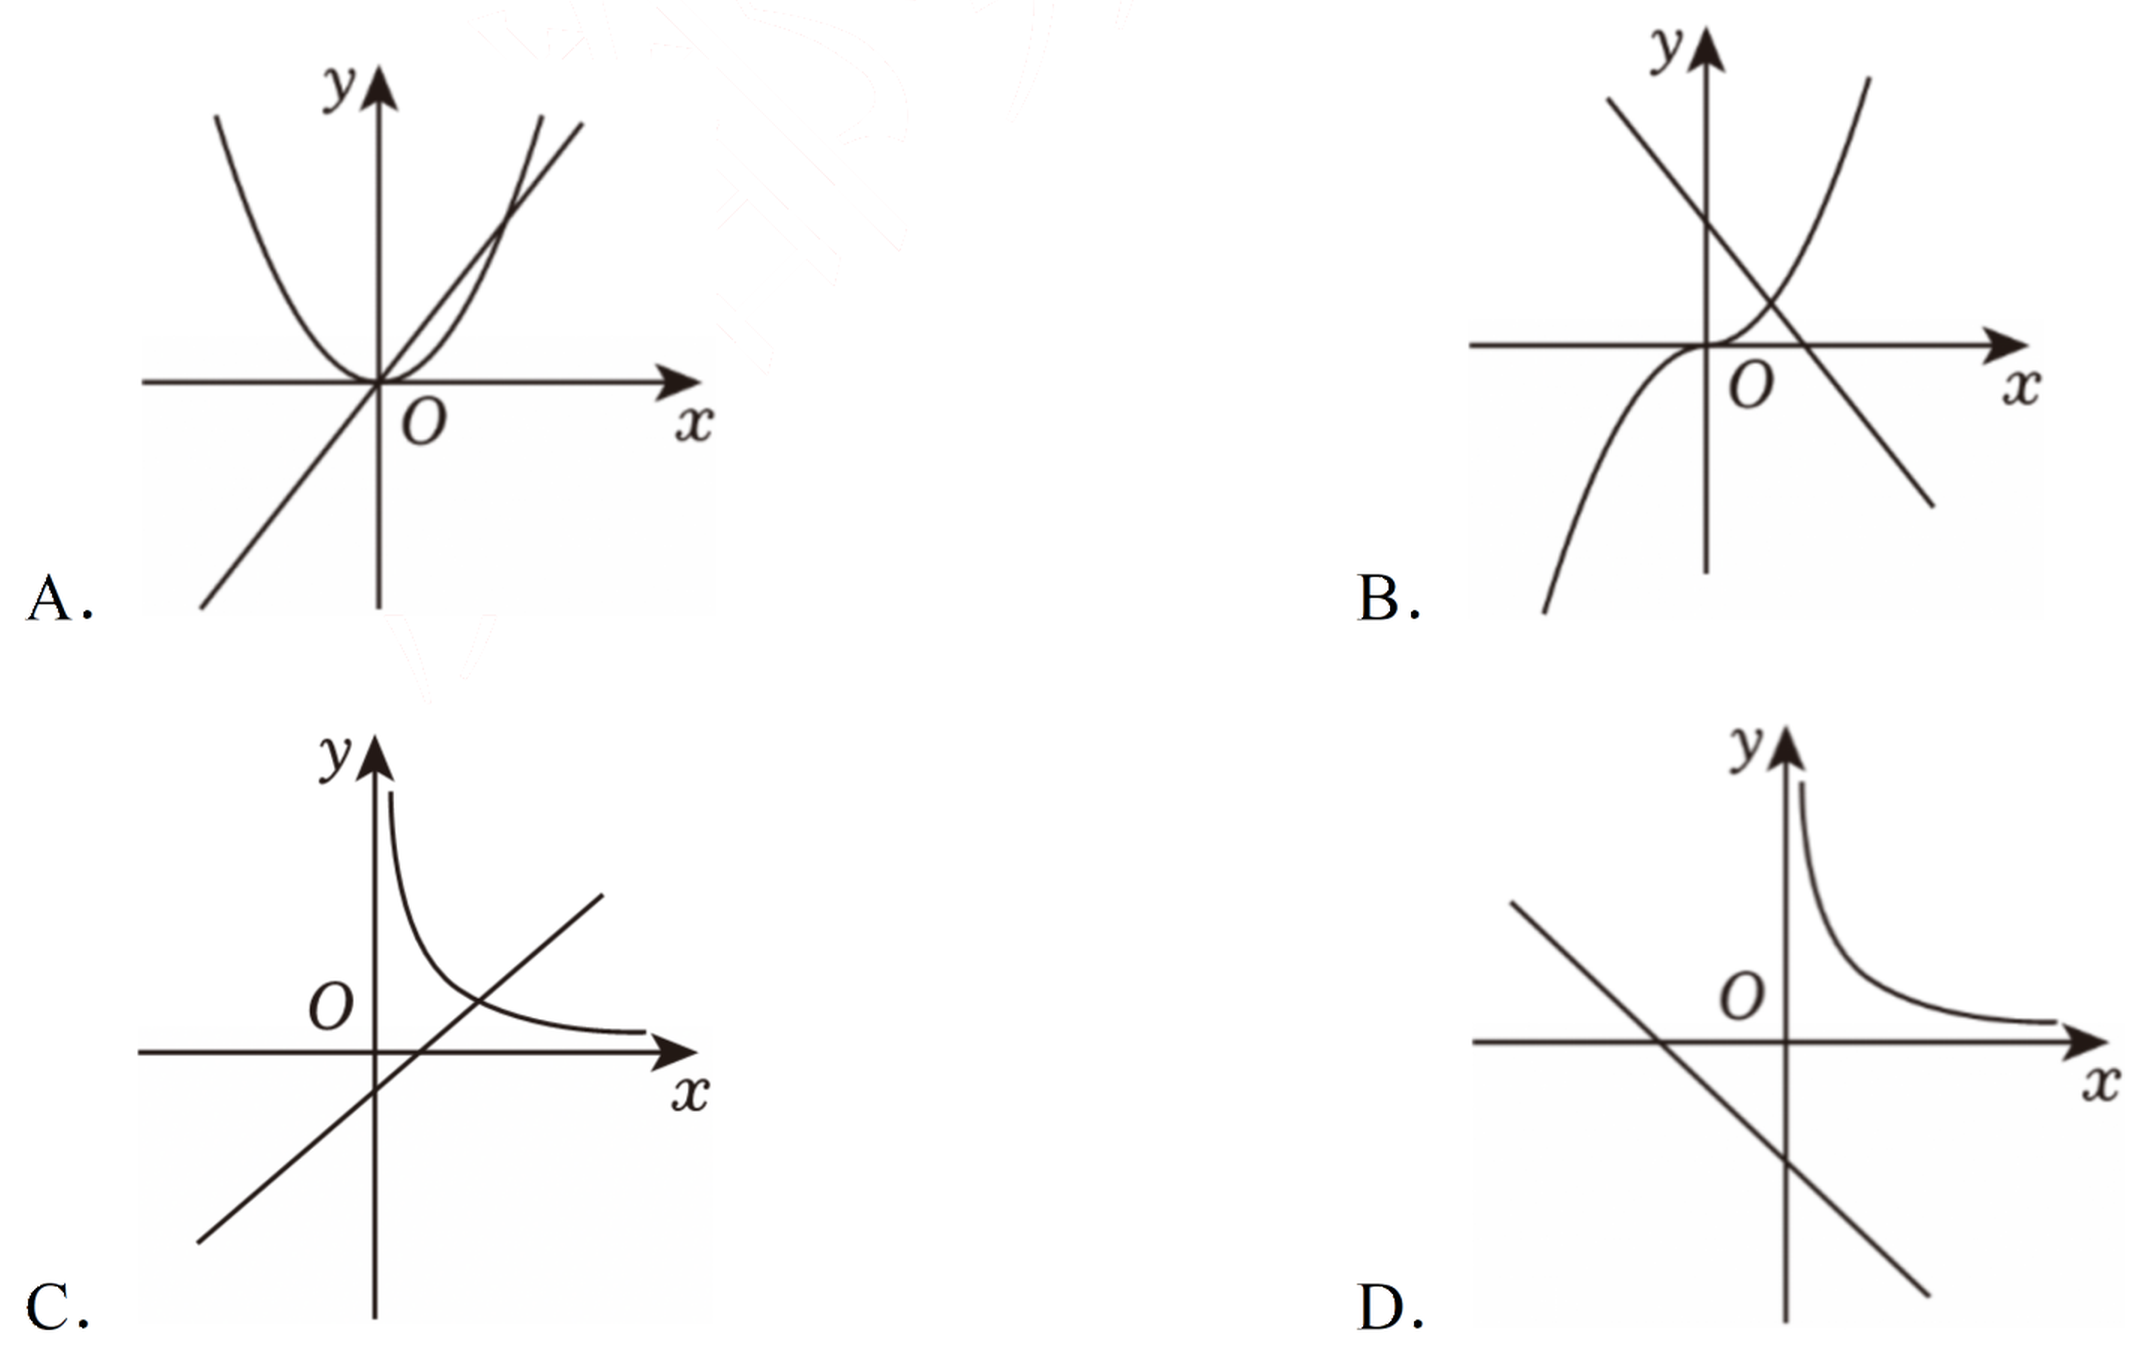
\includegraphics[width=0.80\textwidth]{figures/gao132_q14.png}
\end{center}

\ifanswer
\solbegin
\step{当 $a>0$ 时，$y=ax-\dfrac1a$ 严格增，当 $a<0$ 时，$y=ax-\dfrac1a$ 严格减，}
\step{对于 $A$，因为 $a\ne0$，所以直线 $y=ax-\dfrac1a$ 不过原点，故 $A$ 错误；}
\step{对于 $B$，由函数 $y=x^a(a\ne0)$ 的图象得 $a>1$，}
\step{由 $y=ax-\dfrac1a$ 的图象得 $a<0$，互相矛盾，故 $B$ 错误；}
\step{对于 $C$，由函数 $y=x^a(a\ne0)$ 的图象得 $a>1$，}
\step{由 $y=ax-\dfrac1a$ 的图象得 $a>0$ 且 $-\dfrac1a<0$，符合题意，故 $C$ 正确；}
\step{对于 $D$，由函数 $y=x^a(a\ne0)$ 的图象得 $a<0$，}
\step{由 $y=ax-\dfrac1a$ 的图象得 $a<0$ 且 $-\dfrac1a<0$，互相矛盾，故 $D$ 错误；}
\step{故选 $C$.}
\solend
\fi

\item 中国的 $5G$ 技术领先世界，在 $5G$ 技术中，最大数据传输速率 $C$ 取决于信道带宽 $W$，$C$ 与 $W$ 满足 $C=W\log_2\left(1+\dfrac SN\right)$，其中 $\dfrac SN$ 称为信噪比（单位：$dB$）. 若不改变带宽 $W$，初始信噪比 $\dfrac SN$ 为 $1000$，那么为了使 $C$ 增加 $30\%$，需要将信噪比 $\dfrac SN$ 从 $1000$ 提升至大约\mbox{（\quad）}

\keepwithprev
A. $5000$\qquad\qquad B. $6000$\qquad\qquad C. $7000$\qquad\qquad D. $8000$

\ifanswer
\solbegin
\step{由题意得 $\dfrac SN=1000$ 时，$C=W\log_2(1+1000)\approx W\log_2 1000$，}
\step{要使 $C$ 增加 $30\%$，则 $(1+30\%)C=W\log_2\left(1+\dfrac SN\right)$，即 $1.3C\approx W\log_2\dfrac SN$，}
\step{所以 $1.3\approx\log_{1000}\dfrac SN=\dfrac{\lg\frac SN}{\lg1000}$，所以 $\lg\dfrac SN=3.9$，所以 $\dfrac SN=10^{3.9}\approx8000$.}
\step{故选 $D$.}
\solend
\fi

\item 对于 $a\in\R$，设非空集合 $A=\left\{x\mid\dfrac{(x^2-930x+a)(x-52)}{x+a}=0\right\}$，记 $A$ 中的所有元素之和为 $S(a)$，所有元素之积为 $T(a)$，则下列说法中，不正确的是\mbox{（\quad）}

\keepwithprev
A. 存在实数 $a$，使得 $S(a)=930$

B. 存在实数 $a$，使得 $T(a)=517$

C. 不存在实数 $a$，使得 $T(a)=0$

D. 恰存在 $1$ 个实数 $a$，使得 $T(a)=-52$

\ifanswer
\solbegin
\step{由分式值为 $0$，得分子为 $0$ 且分母不为 $0$，}
\step{分子 $(x^2-930x+a)(x-52)=0$ 的根为 $x=52$}
\step{及方程 $x^2-930x+a=0$ 的两根 $x_1$，$x_2$，}
\step{由根与系数的关系得 $x_1+x_2=930$，$x_1\cdot x_2=a$，}
\step{分母限制 $x\ne-a$，需要剔除等于 $-a$ 的根，}
\step{选项 $A$，取 $a=-52$，$x=52$ 为增根舍去，集合 $A=\{x_1,x_2\}$，}
\step{元素之和 $S(a)=930$，故 $A$ 正确；}
\step{选项 $B$，当无增根时，$T(a)=52a$，令 $52a=517$，得 $a=\dfrac{517}{52}$，}
\step{验证无增根，存在这样的 $a$，故 $B$ 正确；}
\step{选项 $C$，若 $T(a)=0$，则 $0\in A$，代入分子得 $a=0$，}
\step{但 $a=0$ 时分母 $x\ne0$，$x=0$ 为增根，$0$ 不能属于集合 $A$，}
\step{故不存在 $a$ 使得 $T(a)=0$，故 $C$ 正确；}
\step{选项 $D$，当无增根时，令 $52a=-52$，得 $a=-1$；}
\step{当 $x=-a$ 是二次方程的根且不等于 $52$ 时，}
\step{令 $52\times(930+a)=-52$，解得 $a=-931$，验证符合条件；}
\step{当 $a=-52$ 时，$x=52$，舍去，}
\step{集合 $A=\{x_1,x_2\}$，$T(a)=a=-52$，得到两个满足条件的 $a$；}
\step{因此存在 $3$ 个满足条件的 $a$，故 $D$ 错误.}
\step{故选 $D$.}
\solend
\fi

\end{enumerate}

\bigsec{三、解答题}

\begin{enumerate}
\setcounter{enumi}{16}

\item 已知全集 $U=\R$，集合 $A=\left\{x\mid\dfrac{x}{x-3}<0\right\}$，$B=\{x\mid(x-a)(x+4-a)<0\}$.

(1) 当 $a=2$ 时，求 $\overline{B}$、$A\cap\overline{B}$；

(2) 若 $A\cap B=A$，求实数 $a$ 的取值范围.

\ifanswer
\solbegin
\step{(1) $\dfrac{x}{x-3}<0$，即 $x(x-3)<0$，解得 $A=\{x\mid0<x<3\}$，}
\step{当 $a=2$ 时，$B=\{x\mid(x-a)(x+4-a)<0\}=\{x\mid-2<x<2\}$，}
\step{则 $\overline{B}=\{x\mid x\leq-2$ 或 $x\geq2\}$，故 $A\cap\overline{B}=\{x\mid2\leq x<3\}$；}
\step{(2) $A\cap B=A$，则 $A\subseteq B$，故 $\begin{cases}a-4\leq0\\a\geq3\end{cases}$，解得 $3\leq a\leq4$，}
\step{故实数 $a$ 的取值范围是 $\{a\mid3\leq a\leq4\}$.}
\solend
\fi

% 第 18 题是"题干 + 图"约 7cm 的一整块，守卫放在 \item 之前
\needvspace{7cm}
\item 如图，$OA$、$OB$ 是两条长度足够长的互相垂直的笔直小路，矩形 $OCPD$ 的顶点 $C$、$D$ 分别在 $OA$、$OB$ 上，且该矩形区域内种满了荷花. 为了让观赏者有更好的观赏体验，现计划经过点 $P$ 修一条小路 $EF$，其中点 $E$ 在小路 $OA$ 上，点 $F$ 在小路 $OB$ 上，并在 $\triangle OEF$ 区域内种满荷花. 已知 $OD=25m$，$OC=40m$，且小路 $EF$ 要完全位于一个以 $O$ 为顶点的，边长为 $100$ m 的正方形内部（包括边界）. 记 $\triangle OEF$ 的面积为 $S$m$^2$.

(1) 设 $EC=x\cdot m$，试用 $x$ 表示 $OF$，并求 $x$ 的取值范围.

(2) 当 $EC$ 的长度为多少时，$S$ 取得最小值？最小值是多少？

\begin{center}
% 图取原卷 07 页截图去粉色水印，3× LANCZOS 放大
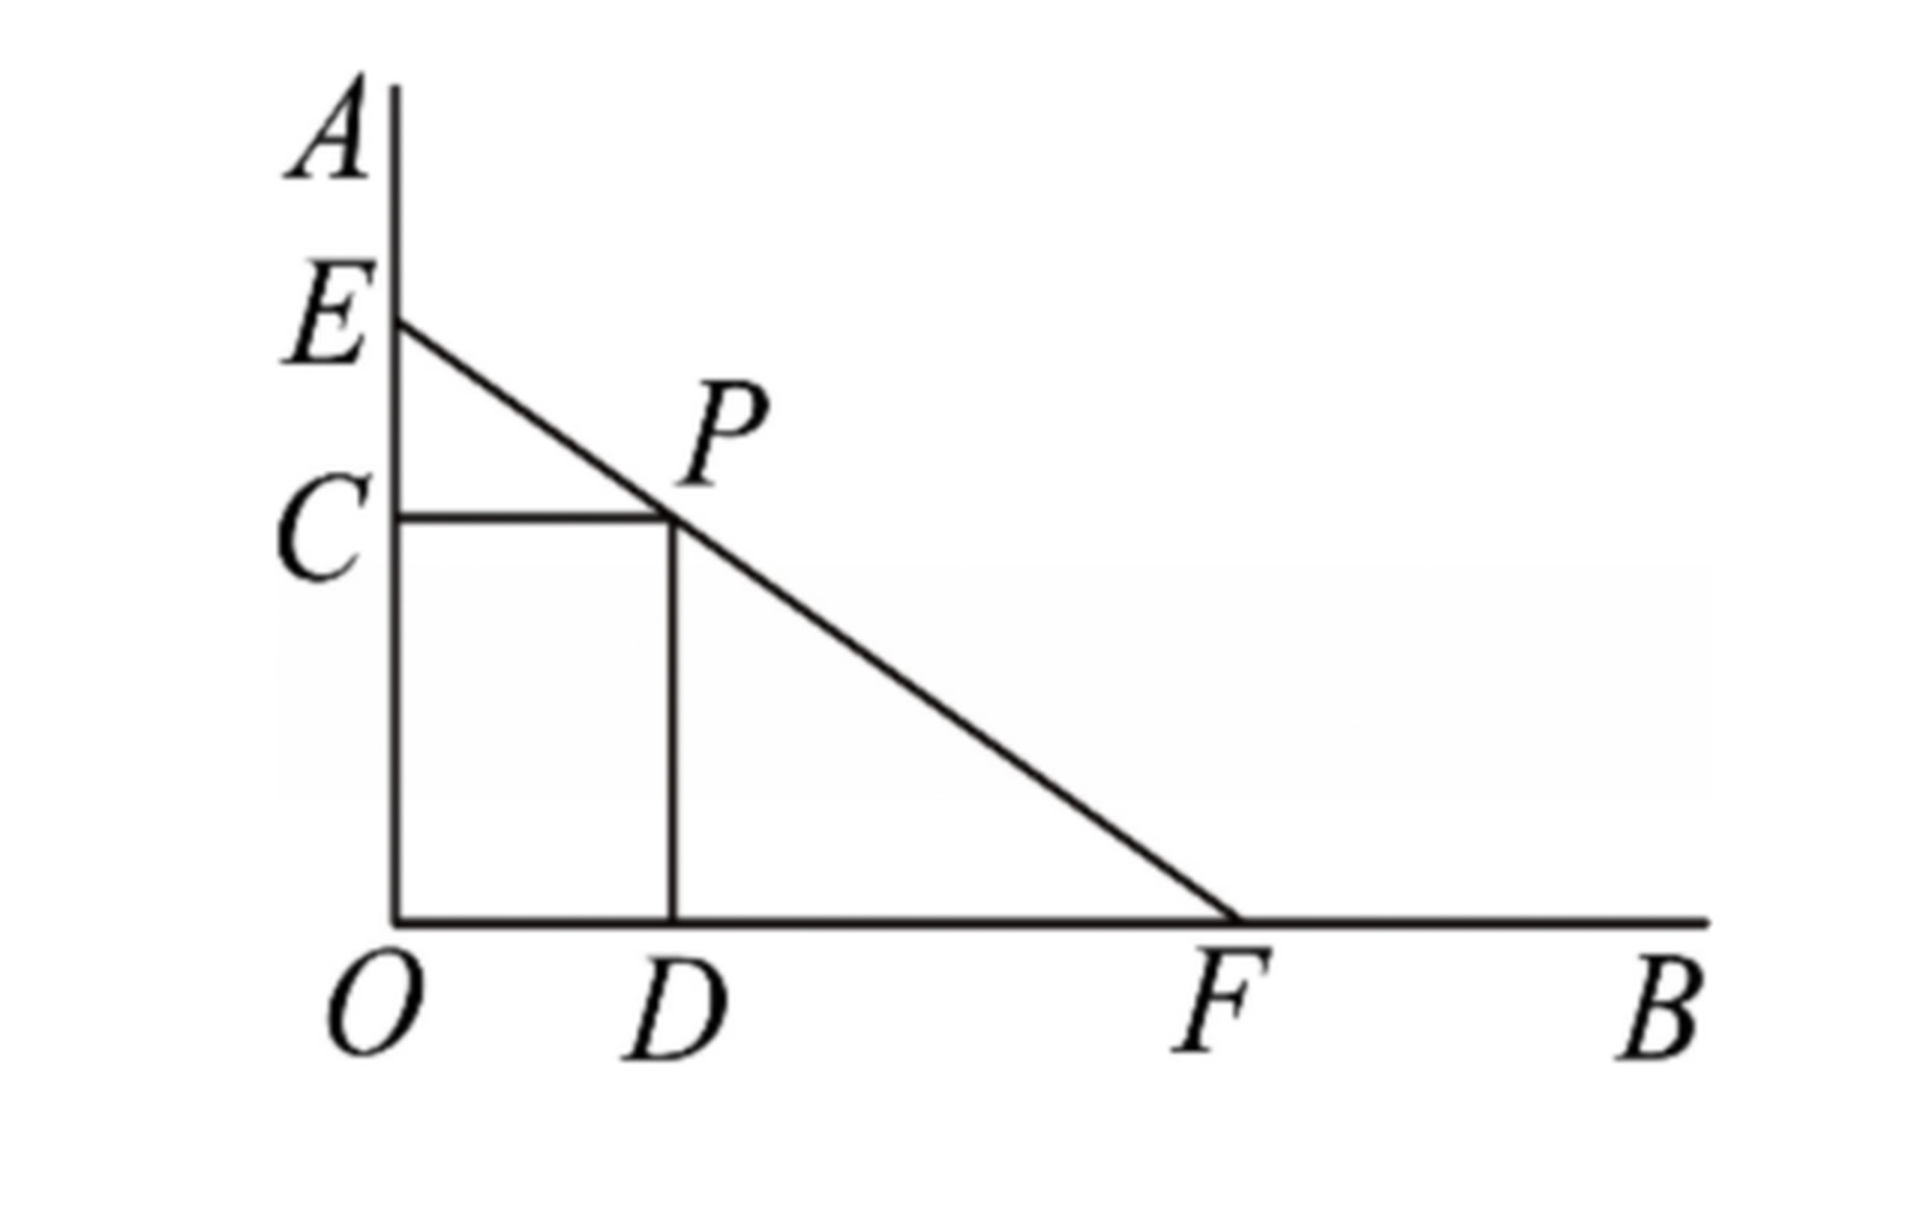
\includegraphics[width=0.32\textwidth]{figures/gao132_q18.png}
\end{center}

\ifanswer
\solbegin
\step{(1) 由题意得 $x\leq60$，}
\step{$\triangle PCE\sim\triangle FDP$，所以 $\dfrac{EC}{CP}=\dfrac{PD}{DF}$，即 $\dfrac{x}{25}=\dfrac{40}{DF}$，得 $DF=\dfrac{1000}{x}$m，}
\step{所以 $OF=OD+DF=\left(25+\dfrac{1000}x\right)$m，}
\step{所以 $25+\dfrac{1000}x\leq100$，解得 $x\geq\dfrac{40}3$；}
\step{综上，$\dfrac{40}3\leq x\leq60$；}
\step{(2) 由 $OE=OC+CE=(40+x)$m，}
\step{所以 $S=\dfrac12 OF\cdot OE=\dfrac12\left(25+\dfrac{1000}x\right)(40+x)$}
\step{$=\dfrac12\left(1000+25x+\dfrac{40000}x+1000\right)$m$^2$，}
\step{由基本不等式得 $S\geq\dfrac12\left(2000+2\sqrt{25x\cdot\dfrac{40000}x}\right)=2000$m$^2$，}
\step{当且仅当 $25x=\dfrac{40000}x$，即 $x=40$ 时取等号，}
\step{故 $EC=40$m 时，$S$ 取得最小值，为 $2000$m$^2$.}
\solend
\fi

\item 已知 $a>0$，$b>0$，请选择适当的方法证明.

(1) 若 $a\ne b$，证明：$a^3+b^3>a^2b+ab^2$；

(2) 若 $ab=1$，证明：$a^2+a<2$ 与 $b^2+b<2$ 不能同时成立.

\ifanswer
\solbegin
\step{(1) 因为 $a>0$，$b>0$，$a\ne b$，}
\step{所以 $a^3+b^3-a^2b-ab^2=a^2(a-b)+b^2(b-a)$}
\step{$=(a^2-b^2)(a-b)=(a-b)^2(a+b)>0$，所以 $a^3+b^3>a^2b+ab^2$.}
\step{(2) 假设 $a^2+a<2$ 与 $b^2+b<2$ 同时成立，所以 $-2<a<1,-2<b<1$，}
\step{又因为 $a>0,b>0$，所以 $0<a<1,0<b<1$，}
\step{所以 $0<ab<1$，这与 $ab=1$ 矛盾，}
\step{故 $a^2+a<2$ 与 $b^2+b<2$ 不可能同时成立.}
\solend
\fi

\item 若设 $M(a,n)=\lvert ax-1\rvert+\lvert ax-2\rvert+\cdots+\lvert ax-n\rvert$ 为曼哈顿扩张距离，它由 $n$ 个绝对值之和组成，其中 $n$ 为正整数.

(1) 若 $M(2,1)\leq5$，求 $x$ 的取值范围；

(2) 若 $k\leq M(2,2)$ 对一切实数 $x$ 恒成立，求实数 $k$ 的取值范围；

(3) $M(2,6)$ 是否存在最小值？若存在，求出该最小值与此时实数 $x$ 的取值范围；若不存在，说明理由.

\ifanswer
\solbegin
\step{(1) $M(2,1)=\lvert2x-1\rvert\leq5$，则不等式可化为 $-5\leq2x-1\leq5$，解得 $-2\leq x\leq3$，}
\step{所以 $x$ 的取值范围为 $[-2,3]$.}
\step{(2) 因为 $k\leq M(2,2)=\lvert2x-1\rvert+\lvert2x-2\rvert$ 对一切实数 $x$ 恒成立，}
\step{又 $\lvert2x-1\rvert+\lvert2x-2\rvert\geq\lvert(2x-1)-(2x-2)\rvert=1$，}
\step{当且仅当 $(2x-1)(2x-2)\leq0$，即 $\dfrac12\leq x\leq1$ 时取等号，}
\step{故 $k\leq1$，所以实数 $k$ 的取值范围为 $(-\infty,1]$.}
\step{(3) $M(2,6)=\lvert2x-1\rvert+\lvert2x-2\rvert+\lvert2x-3\rvert+\lvert2x-4\rvert+\lvert2x-5\rvert+\lvert2x-6\rvert$}
\step{$=2\left(\left\lvert x-\dfrac12\right\rvert+\lvert x-1\rvert+\left\lvert x-\dfrac32\right\rvert+\lvert x-2\rvert+\left\lvert x-\dfrac52\right\rvert+\lvert x-3\rvert\right)$，}
\step{其中 $\left\lvert x-\dfrac12\right\rvert+\lvert x-1\rvert+\left\lvert x-\dfrac32\right\rvert+\lvert x-2\rvert+\left\lvert x-\dfrac52\right\rvert+\lvert x-3\rvert$ 的几何意义为}
\step{在数轴上一点 $x$ 到 $\dfrac12,1,\dfrac32,2,\dfrac52,3$ 的距离之和，}
\step{要想距离之和最小，其中 $x\in\left[\dfrac12,3\right]$ 时，$\left\lvert x-\dfrac12\right\rvert+\lvert x-3\rvert$ 取得最小值，}
\step{当 $x\in\left[1,\dfrac52\right]$ 时，$\lvert x-1\rvert+\left\lvert x-\dfrac52\right\rvert$ 取得最小值，}
\step{当 $x\in\left[\dfrac32,2\right]$ 时，$\left\lvert x-\dfrac32\right\rvert+\lvert x-2\rvert$ 取得最小值，}
\step{综上，当 $x\in\left[\dfrac32,2\right]$ 时，$\left\lvert x-\dfrac12\right\rvert+\lvert x-1\rvert+\left\lvert x-\dfrac32\right\rvert+\lvert x-2\rvert+\left\lvert x-\dfrac52\right\rvert+\lvert x-3\rvert$}
\step{取得最小值，最小值为 $3-\dfrac12+\dfrac52-1+2-\dfrac32=\dfrac92$，}
\step{故 $M(2,6)=2\left(\left\lvert x-\dfrac12\right\rvert+\lvert x-1\rvert+\left\lvert x-\dfrac32\right\rvert+\lvert x-2\rvert+\left\lvert x-\dfrac52\right\rvert+\lvert x-3\rvert\right)$ 的}
\step{最小值为 $9$.}
\solend
\fi

\item 已知集合 $A=\{a_1,a_2,\cdots,a_n\}(0\leq a_1<a_2<\cdots<a_n,n\in\N,n\geq3)$ 具有性质 $Q$：对任意 $i,j(1\leq i\leq j\leq n)$，$a_i+a_j$ 与 $a_j-a_i$ 至少有一个属于集合 $A$；

(1) 判断集合 $M=\{0,2,4\}$ 与 $N=\{2,3,4\}$ 是否具有性质 $Q$，并说明理由；

(2) 已知 $A=\{a_1,a_2,a_3\}$ 具有性质 $Q$，当 $a_2=2026$ 时，求集合 $A$；

(3) 已知 $B=\{b_1,b_2,\cdots,b_{2026}\}$ 具有性质 $Q$，求 $\dfrac{b_1+b_2+\cdots+b_{2026}}{b_{2026}}$ 的值；

\ifanswer
\solbegin
\step{(1) 集合 $M=\{0,2,4\}$ 中，}
\step{因为 $0+2\in M,0+4\in M,4-2\in M,0\pm0=0\in M$，}
\step{$2+2=4\in M,2-2=0\in M,4-4=0\in M$，所以集合 $M$ 具有性质 $Q$；}
\step{集合 $N=\{2,3,4\}$ 中，因为 $3+3=6\notin N,3-3=0\notin N$，}
\step{所以集合 $N$ 不具有性质 $Q$.}
\step{(2) 因为 $a_1<a_2<a_3$，且 $A=\{a_1,a_2,a_3\}$ 具有性质 $Q$，}
\step{所以 $a_3+a_3\notin A,a_3-a_3=0\in A$，则 $a_1=0$，}
\step{又因为 $a_2+a_3>a_3$，所以 $a_2+a_3\notin A$，则 $a_3-a_2\in A$，}
\step{由集合的互异性得 $a_3-a_2=a_2$，而 $a_2=2026$，所以 $a_3=4052$，}
\step{故 $A=\{0,2026,4052\}$；}
\step{(3) 先证明一般结论：$A=\{a_1,a_2,\cdots,a_n\}(0\leq a_1<a_2<\cdots<a_n,n\in\N,n\geq3)$}
\step{具有性质 $Q$，则 $a_1+a_2+a_3+\cdots+a_n=\dfrac n2 a_n$.}
\step{因为 $A=\{a_1,a_2,\cdots,a_n\}(0\leq a_1<a_2<\cdots<a_n,n\in\N,n\geq3)$ 具有性质 $Q$，}
\step{所以 $a_n+a_n\notin A$，则 $a_n-a_n=0\in A$，则 $a_1=0$.}
\step{又因为 $0\leq a_1<a_2<\cdots<a_n$，所以 $0\leq a_n-a_n<a_n-a_{n-1}<\cdots<a_n-a_1$，}
\step{又因为 $a_n+a_{n-i}>a_n(i=1,2,\cdots,n-1)$，所以 $a_n+a_{n-i}\notin A$，}
\step{则 $a_n-a_{n-i}\in A$，}
\step{所以 $a_1=a_n-a_n,a_2=a_n-a_{n-1},a_3=a_n-a_{n-2},\cdots,a_n=a_n-a_1$.}
\step{所以 $a_1+a_2+a_3+\cdots+a_n$}
\step{$=(a_n-a_n)+(a_n-a_{n-1})+(a_n-a_{n-2})+\cdots+(a_n-a_1)$，}
\step{即 $a_1+a_2+a_3+\cdots+a_n=\dfrac n2 a_n$，}
\step{所以 $B=\{b_1,b_2,\cdots,b_{2026}\}$ 具有性质 $Q$，则 $b_1+b_2+\cdots+b_{2026}=\dfrac{2026}{2}b_{2026}$，}
\step{所以 $\dfrac{b_1+b_2+\cdots+b_{2026}}{b_{2026}}=\dfrac{2026}{2}=1013$.}
\solend
\fi

\end{enumerate}

% 行数复核：逐题数 \step 条数，合计 144 条（Q3：4；Q4：1；Q5：4；Q6：2；Q7：9；Q8：2；
% Q9：3；Q10：6；Q11：9；Q12：9；Q13：0；Q14：9；Q15：4；Q16：19；Q17：5；Q18：11；
% Q19：7；Q20：17；Q21：23），与原卷印刷行逐题相等（cases 块作一个印刷行计）。
% 第 13 题只印括号内答案、提 \ans{}，不计入 \step 账；第 14—16 题答案在解析末句，
% 括号内留空、不另提 \ans{}。

\end{document}
"
%
% 原始材料：微信公众号"魔都数学加油站"文章，作者破晓，2026-11-14 19:00 发布；
% 连载"27学年高一132"，原文标题"27学年高一132——2026-2027年上海市川沙中学高一上期中"；
% 原文链接：https://mp.weixin.qq.com/s/VBG01CrUNMIYWWHhSfz8JQ。
% 正文为 11 张 PNG 页（01、04、06、07、09、11 为 2560x3620，02、03、05、08、10 为 4762x6735），
% 题目下印有【解析】，为讲评版。题目、解析均据原图转录；
% 卷面粉红色水印"魔都数学加油站"及公众号页脚未录入。全卷 2 幅插图：第 14 题四幅坐标图选项、
% 第 18 题矩形 OCPD 与小路 EF 示意图，均取原卷 04／07 页截图去水印。
%
% 卷首标题：原卷印作"2026-2027 年川沙中学高一上期中"（公众号标题中的"上海市"
% 卷面标题行没有，本稿照卷面），年份区间按全稿惯例排 en dash；原卷未印副标题，
% 本卷为期中卷、跨集合与常用逻辑用语／不等式／函数三章，按题目内容标为
% "集合与常用逻辑用语、不等式、函数"（与 125／126／128／129／131 同期中卷口径相同）：
% 集合与逻辑见 Q5、Q6、Q17、Q21，不等式见 Q3、Q4、Q9、Q10、Q12、Q13、Q15、Q16、Q19，
% 函数（幂函数、指数／对数、基本不等式应用）见 Q7、Q8、Q11、Q14、Q18、Q20。
%
% 题号体例：本卷共 19 题——一、填空题 3—12（10 题）、二、选择题 13—16（4 题）、
% 三、解答题 17—21（5 题）。三节分别 \setcounter{enumi}{2}／{12}／{16}。
%
% 与原卷的排版差异：
%   ① 原文从第 3 题起，本稿保留原题号（见上"题号体例"）；
%   ② 原卷每题下直接印【解析】，本稿按全稿惯例置于答案版；第 13 题答案 D 印在题干
%      括号内、无独立答案段，按 高一37／52／53／55／63／64／128／131 成例括号留空、
%      另提 \ans{$D$}；第 14—16 题答案在解析末句"故选 …"，括号内留空、不另提 \ans{}；
%   ③ 原卷未印副标题，本稿按"知识模块"口径补出；
%   ④ 原卷填空横线按全稿惯例排为 \blankline[4.4em]；选择题括号排 \mbox{（\quad）}、
%      选项段前按惯例加 \keepwithprev；解答题不留作答区（原卷为讲评版，与 109—131 同）；
%   ⑤ 原卷数集排斜体 $R^+$／$R$／$Z$／$N$，按全稿惯例改 \R^+／\R／\Z／\N；
%      绝对值排 \lvert…\rvert，集合描述竖线排 \mid；不等号按全稿惯例排 \leqslant／\geqslant；
%      补集照原卷上划线排 \overline{B}；
%   ⑥ 子题标号 (1)(2)(3) 原卷用半角括号，照录；第 14 题四幅坐标图选项按原卷 2×2 排布
%      合并裁为一张 \includegraphics（未用 TikZ 重绘，以保证与原卷一致），题前加
%      \needvspace{9cm} 守卫；第 18 题图取 07 页截图，题前按惯例加 \needvspace{7cm} 守卫
%      （照 高一120／127／129／131 成例），两者守卫都放在 \item 之前；
%   ⑦ 原卷 Q7 解析跨 01—02 页、Q10 解析跨 02—03 页、Q12 解析跨 03—04 页、
%      Q14 解析跨 04—05 页、Q16 解析在 06 页、Q18 解析跨 07—08 页、
%      Q20 解析跨 08—09 页、Q21 解析跨 10—11 页，本稿按题合并连续排版；
%      末页第 11 页为 Q21 (3) 解析的续尾，按实际印刷行单列。
%
% 判别式字形：第 10 题 $\triangle=4(a-1)^2+16(a-1)<0$、第 11 题
%   $\triangle=4(m-2)^2-4(m^2-3m+3)=-4m+4>0$ 两处原卷均排 $\triangle$（等边、扁），
%   逐处放大核对、字形一致，照录 \triangle；与 高一129／131 同题排 $\Delta$（等腰、高）不同。
%   全卷 \triangle 兼作第 18 题「$\triangle PCE\sim\triangle FDP$」「$\triangle OEF$」的几何
%   三角形记号，全卷未出现 \Delta。
%
% 子集符号：第 5 题解析 $B\subseteq A$、第 17 题 (2) 解析 $A\subseteq B$ 均印带下划线，
%   照录 \subseteq；全卷未出现单线 \subset。
%
% 原卷存疑照录：
%   第 9 题题干作"充分非必要条件"、解析作"充分不必要条件"，措辞不同，照录；
%   第 10 题解析"当 $a-1=0$ 时，$-4\geq0$，不等式不成立，$a=1$ 满足题意"照录；
%   第 11 题解析"所以 $2(m-1)+\dfrac1{m-1}\leq-2\sqrt2$"由上一行 $2(1-m)+\dfrac1{1-m}\geq2\sqrt2$
%     直接变号得到，照录；
%   第 12 题解析"由 $x\in Z$，$-7<-2\sqrt{10}<-6$"与"即 $k^2+7k+10\leq0$，解得 $-5\leq k\leq-2$"照录；
%   第 16 题解析"令 $52\times(930+a)=-52$，解得 $a=-931$"（按式应为 $a=-931$ 之外的解）照录；
%   第 19 题 (2) 解析"所以 $-2<a<1,-2<b<1$"数学式内半角逗号，照录；
%   第 20 题 (3) 解析"最小值为 $3-\dfrac12+\dfrac52-1+2-\dfrac32=\dfrac92$"与
%     "故 $M(2,6)=\dots$ 的最小值为 9"两处结论并列，照录；
%   第 21 题 (1) 解析"$0+2\in M,0+4\in M,4-2\in M,0\pm0=0\in M$"、
%     "$2+2=4\in M,2-2=0\in M,4-4=0\in M$"、(3) 各连写等式内半角逗号，照录；
%   第 21 题 (3) 解析"即 $a_1+a_2+a_3+\cdots+a_n=\dfrac n2 a_n$，"句末用半角逗号，照录。
%
% 行数复核：见文末"行数复核"注（逐题 \step 条数与原卷印刷行逐题相等，cases 块作一个印刷行计）。
%   第 13 题只印括号内答案、提 \ans{}，不计入 \step 账；第 14—16 题答案在解析末句，
%   括号内留空、不另提 \ans{}。
%
\documentclass[a4paper,11pt]{article}
\usepackage{common}

\begin{document}

\examtitlest[3]{2026--2027 年川沙中学高一上期中}{集合与常用逻辑用语、不等式、函数}

\bigsec{一、填空题}

\begin{enumerate}
\setcounter{enumi}{2}

\item 已知 $a$、$b\in\R^+$ 且 $ab=2$，则 $a+2b$ 的最小值为\blankline[4.4em].

\ifanswer
\solbegin
\step{因为 $a\in\R^+$，$b\in\R^+$ 且 $ab=2$，}
\step{由基本不等式得 $a+2b\geq2\sqrt{a\cdot2b}=2\sqrt{2ab}=2\sqrt4=4$.}
\step{等号当且仅当 $a=2b$ 时成立，结合 $ab=2$ 解得 $b=1$，$a=2$，}
\step{所以 $a+2b$ 的最小值为 $4$.}
\solend
\fi

\item 如果幂函数 $f(x)=(m^2-3m-3)x^{m^2+m-3}$ 在 $(0,+\infty)$ 上是增函数，则实数 $m=$\blankline[4.4em].

\ifanswer
\solbegin
\step{由已知得 $\begin{cases}m^2-3m-3=1\\m^2+m-3>0\end{cases}$，所以 $m=4$.}
\solend
\fi

\item 已知集合 $A=\{1,2\}$，集合 $B=\{x\mid ax=6\}$，若 $A\cup B=A$，则 $a$ 的所有取值构成的集合为\blankline[4.4em].

\ifanswer
\solbegin
\step{因为 $A\cup B=A$，所以 $B\subseteq A$，}
\step{当 $a=0$ 时，$B=\varnothing$，满足 $B\subseteq A$；}
\step{当 $a\ne0$ 时，$B=\left\{\dfrac6a\right\}$，则 $\dfrac6a=1$ 或 $\dfrac6a=2$，解得 $a=6$ 或 $a=3$，}
\step{综上所述，$a$ 的所有取值构成的集合为 $\{0,3,6\}$.}
\solend
\fi

\item 设全集为 $\R$，$A=\{y\mid y=-x^2+2x+1\}$，$B=\{x\mid y=\ln(x-1)\}$，则 $A\cap B=$\blankline[4.4em].

\ifanswer
\solbegin
\step{$A=\{y\mid y=-x^2+2x+1\}=\{y\mid y=-(x-1)^2+2\}=\{y\mid y\leq2\}$，}
\step{$B=\{x\mid y=\ln(x-1)\}=\{x\mid x>1\}$，则 $A\cap B=(1,2]$.}
\solend
\fi

\item 已知 $x\in\R$，则方程 $\lvert 6-x\rvert+\lvert 6x-3\rvert=\lvert 5x+3\rvert$ 的解集为\blankline[4.4em].

\ifanswer
\solbegin
\step{当 $x<-\dfrac35$ 时，$6-x>0$，$6x-3<0$，$5x+3<0$，}
\step{原方程为 $6-x-6x+3=-5x-3$，解得 $x=6$，不满足 $x<-\dfrac35$；}
\step{当 $-\dfrac35\leq x\leq\dfrac12$ 时，$5x+3\geq0$，$6x-3<0$，$6-x>0$，}
\step{原方程为 $6-x+3-6x=5x+3$，解得 $x=\dfrac12$；}
\step{当 $\dfrac12<x\leq6$ 时，$5x+3>0$，$6x-3>0$，$6-x\geq0$，}
\step{原方程为 $6-x+6x-3=5x+3$，即 $0=0$，恒成立，所以 $\dfrac12<x\leq6$；}
\step{当 $x>6$ 时，$5x+3\geq0$，$6x-3>0$，$6-x<0$，}
\step{原方程为 $x-6+6x-3=5x+3$，解得 $x=6$，不满足 $x>6$；}
\step{综上 $\dfrac12\leq x\leq6$，所以原方程的解集为 $\left\{x\mid\dfrac12\leq x\leq6\right\}$.}
\solend
\fi

\item 已知 $\log_2 3=a,2^b=7$，用 $a,b$ 表示 $\log_{42}56$ 为\blankline[4.4em].

\ifanswer
\solbegin
\step{$\log_{42}56=\dfrac{\log_2 56}{\log_2 42}=\dfrac{\log_2(7\times8)}{\log_2(6\times7)}=\dfrac{\log_2 7+\log_2 8}{\log_2 6+\log_2 7}$}
\step{$=\dfrac{\log_2 7+\log_2 2^3}{\log_2 2+\log_2 3+\log_2 7}=\dfrac{b+3}{1+a+b}$.}
\solend
\fi

\item 已知 $\dfrac13<x<\dfrac12$ 是不等式 $\lvert x-m\rvert<1$ 成立的充分非必要条件，则 $m$ 的取值范围是\blankline[4.4em].

\ifanswer
\solbegin
\step{因为 $\lvert x-m\rvert<1$，所以 $-1<x-m<1$，所以 $m-1<x<m+1$，}
\step{所以 $m-1<x<m+1$ 成立的充分不必要条件是 $\dfrac13<x<\dfrac12$，}
\step{所以 $\begin{cases}m-1\leq\dfrac13\\m+1\geq\dfrac12\end{cases}$，解得 $-\dfrac12\leq m\leq\dfrac43$，故 $m$ 的取值范围是 $\left[-\dfrac12,\dfrac43\right]$.}
\solend
\fi

\item 若关于 $x$ 的不等式 $(a-1)x^2+2(a-1)x-4\geq0$ 的解集为空集，则 $a$ 的取值范围是\blankline[4.4em].

\ifanswer
\solbegin
\step{关于 $x$ 的不等式 $(a-1)x^2+2(a-1)x-4\geq0$ 的解集为 $\varnothing$，}
\step{当 $a-1=0$ 时，$-4\geq0$，不等式不成立，$a=1$ 满足题意；}
\step{当 $a-1>0$ 时，$a>1$，不等式的解集不为空集，不满足题意；}
\step{当 $a-1<0$ 时，$a<1$，当 $\triangle=4(a-1)^2+16(a-1)<0$ 时，即 $(a-1)(a+3)<0$，}
\step{解得 $-3<a<1$，满足题意；}
\step{综上，实数 $a$ 的取值范围是 $\{a\mid-3<a\leq1\}$.}
\solend
\fi

\item 已知关于 $x$ 的方程 $x^2+2(m-2)x+m^2-3m+3=0$ 有两个不相等的实数根 $x_1$、$x_2$，则 $\dfrac{mx_1}{x_1-1}+\dfrac{mx_2}{x_2-1}-\dfrac{2}{x_1+x_2-2}$ 的最大值为\blankline[4.4em].

\ifanswer
\solbegin
\step{关于 $x$ 的方程 $x^2+2(m-2)x+m^2-3m+3=0$ 有两个不相等的实数根 $x_1$、$x_2$，}
\step{则 $\triangle=4(m-2)^2-4(m^2-3m+3)=-4m+4>0$，得 $m<1$，}
\step{且 $x_1+x_2=-2(m-2)$，$x_1x_2=m^2-3m+3$，}
\step{$\dfrac{mx_1}{x_1-1}+\dfrac{mx_2}{x_2-1}-\dfrac{2}{x_1+x_2-2}=\dfrac{m[2x_1x_2-(x_1+x_2)]}{x_1x_2-(x_1+x_2)+1}+\dfrac1{m-1}$}
\step{$=\dfrac{2m(m-1)^2}{m^2-m}+\dfrac1{m-1}=2(m-1)+\dfrac1{m-1}$，}
\step{又因为 $m<1$，所以 $m-1<0$，则 $1-m>0$，}
\step{所以 $2(1-m)+\dfrac1{1-m}\geq2\sqrt{2(1-m)\cdot\dfrac1{1-m}}=2\sqrt2$，}
\step{当且仅当 $2(1-m)=\dfrac1{1-m}$ 时，即 $m=1-\dfrac{\sqrt2}2$ 时取等号，}
\step{所以 $2(m-1)+\dfrac1{m-1}\leq-2\sqrt2$，即 $\dfrac{mx_1}{x_1-1}+\dfrac{mx_2}{x_2-1}-\dfrac2{x_1+x_2-2}$ 的最大值为 $-2\sqrt2$.}
\solend
\fi

\item 若使集合 $A=\{x\mid(kx-k^2-10)(x-1)>0,x\in\Z\}$ 中的元素个数最少，则实数 $k$ 的取值范围是\blankline[4.4em].

\ifanswer
\solbegin
\step{由题意集合 $A=\{x\mid(kx-k^2-10)(x-1)>0,\ x\in\Z\}$，}
\step{$k=0$ 时，不等式解得 $x<1$，有无数个整数解；}
\step{$k\ne0$ 时，则不等式变形为 $k\left(x-k-\dfrac{10}k\right)(x-1)>0$，}
\step{当 $k>0$ 时，$k+\dfrac{10}k\geq2\sqrt{10}$，仅当 $k=\sqrt{10}$ 时等号成立，}
\step{此时不等式解得 $x>k+\dfrac{10}k$ 或 $x<1$，有无数个整数解；}
\step{当 $k<0$ 时，$k+\dfrac{10}k=-\left[(-k)+\left(-\dfrac{10}k\right)\right]\leq-2\sqrt{10}$，仅当 $k=-\sqrt{10}$ 时等号成立，}
\step{此时不等式解得 $k+\dfrac{10}k<x<1$，}
\step{由 $x\in\Z$，$-7<-2\sqrt{10}<-6$，要使集合 $A$ 中的元素最少，则 $k+\dfrac{10}k\geq-7$，}
\step{即 $k^2+7k+10\leq0$，解得 $-5\leq k\leq-2$，故实数 $k$ 的取值范围是 $[-5,-2]$.}
\solend
\fi

\end{enumerate}

\bigsec{二、选择题}

\begin{enumerate}
\setcounter{enumi}{12}

\item 下列说法正确的是\mbox{（\quad）}

\keepwithprev
A. 若 $a>b$，则 $\dfrac1a<\dfrac1b$\qquad\qquad B. 若 $a>b$，$c>d$，则 $ac>bd$

C. 若 $a>b$，则 $ac^2>bc^2$\qquad\qquad D. 若 $ac^2>bc^2$，则 $a>b$

\ifanswer
\ans{$D$}
\fi

% 第 14 题四幅坐标图选项是一整块，守卫放在 \item 之前
\needvspace{9cm}
\item 在同一坐标系内，函数 $y=x^a(a\ne0)$ 和 $y=ax-\dfrac1a$ 的图象可能是\mbox{（\quad）}

\keepwithprev
\begin{center}
% 四幅坐标图选项取原卷 04 页截图去粉色水印，按原卷 2×2 排布合并为一张
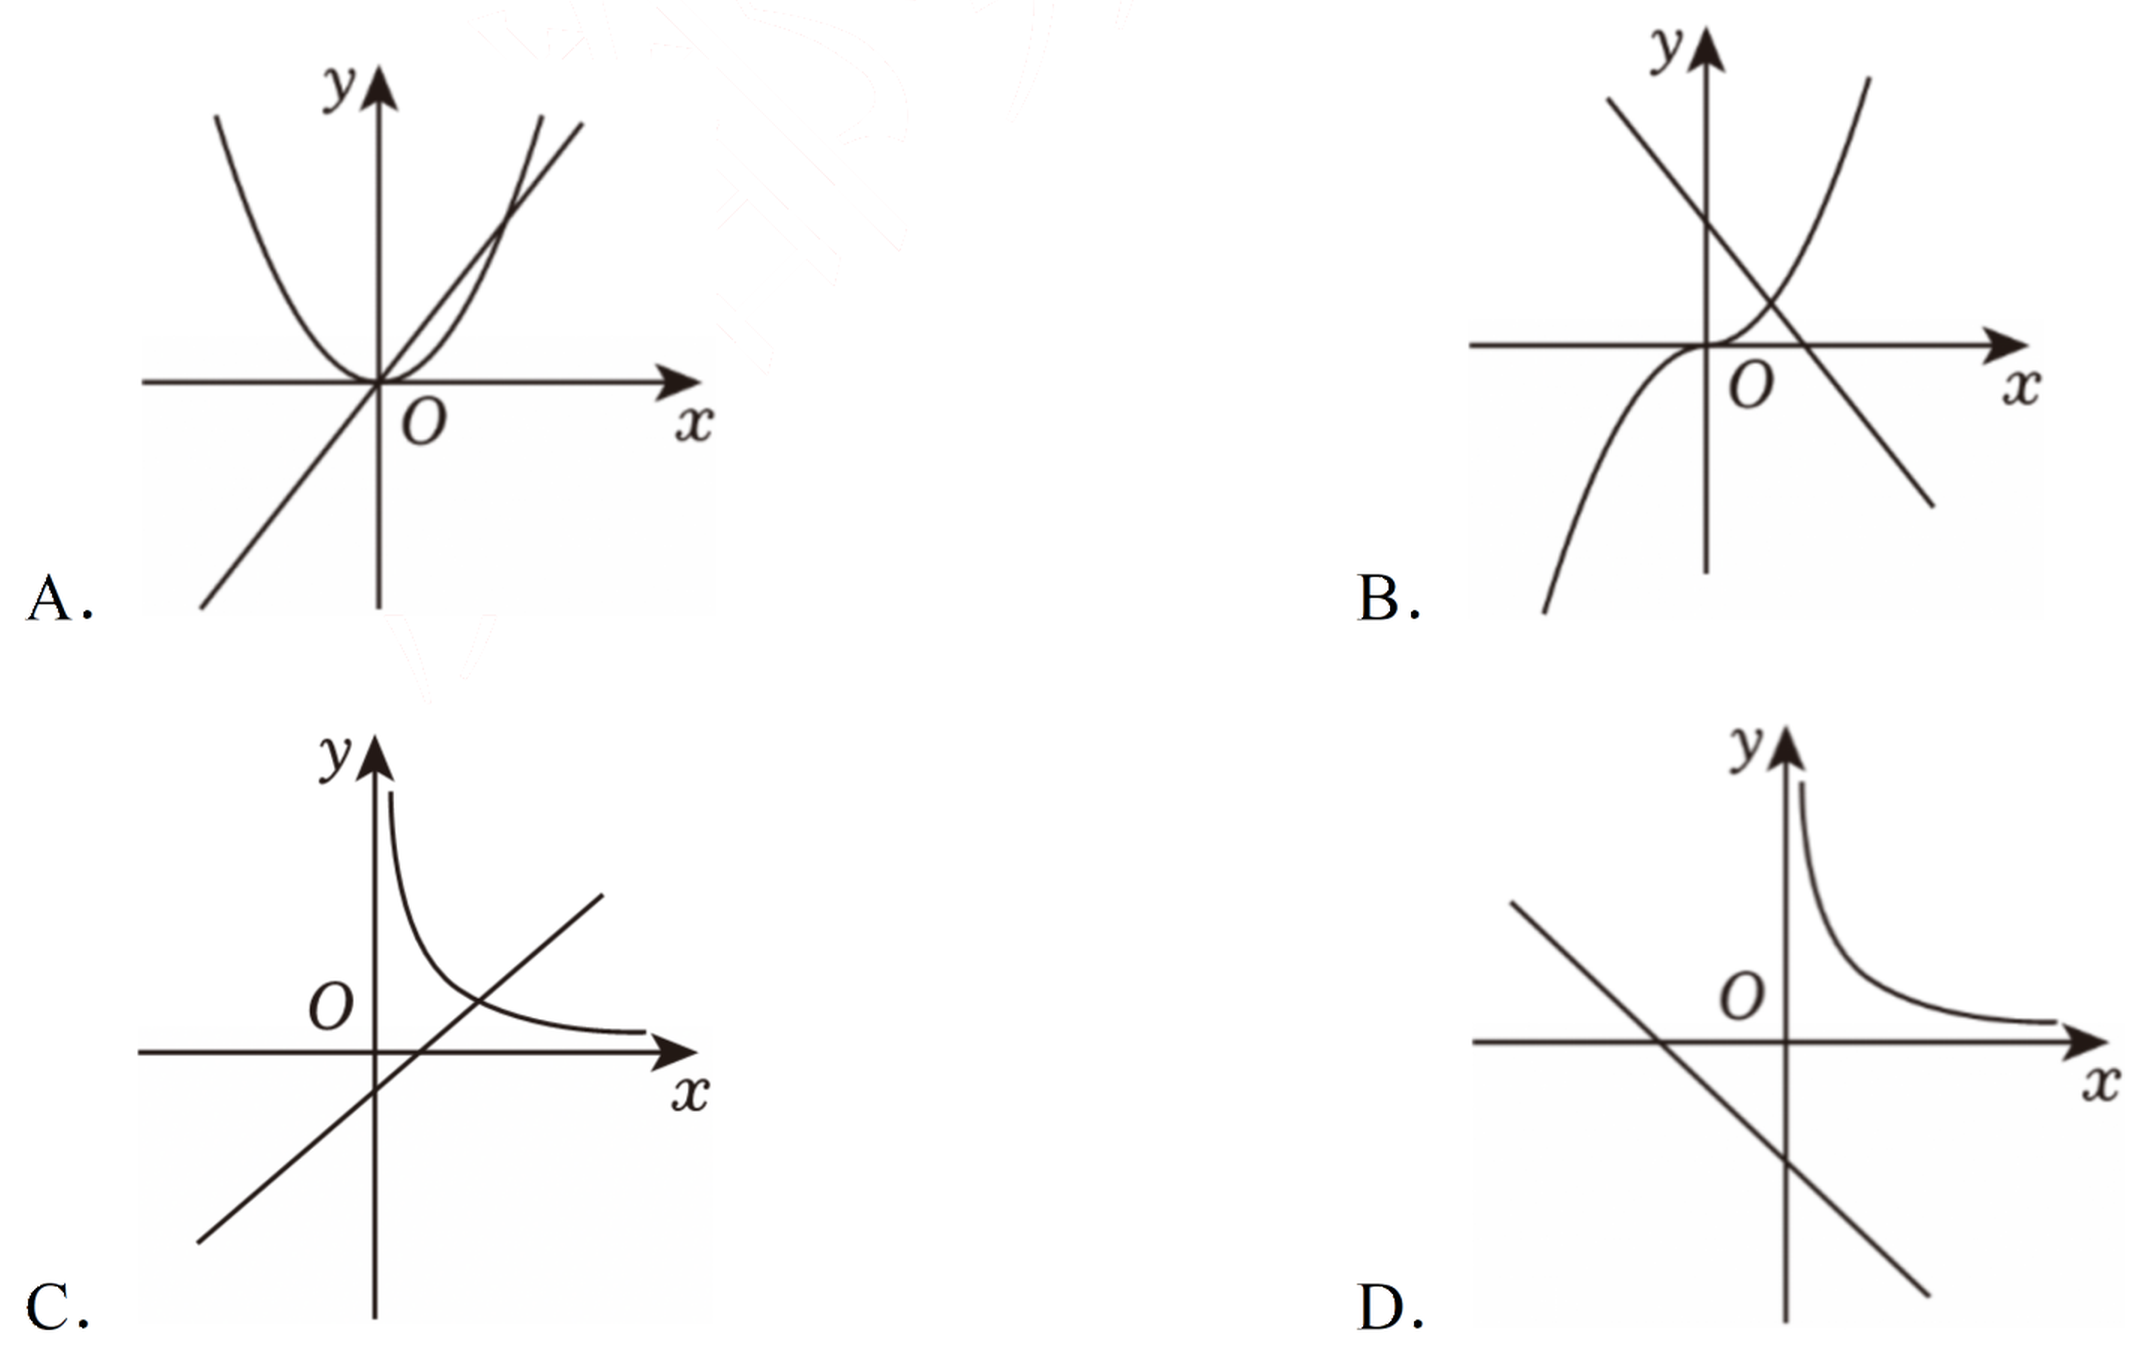
\includegraphics[width=0.80\textwidth]{figures/gao132_q14.png}
\end{center}

\ifanswer
\solbegin
\step{当 $a>0$ 时，$y=ax-\dfrac1a$ 严格增，当 $a<0$ 时，$y=ax-\dfrac1a$ 严格减，}
\step{对于 $A$，因为 $a\ne0$，所以直线 $y=ax-\dfrac1a$ 不过原点，故 $A$ 错误；}
\step{对于 $B$，由函数 $y=x^a(a\ne0)$ 的图象得 $a>1$，}
\step{由 $y=ax-\dfrac1a$ 的图象得 $a<0$，互相矛盾，故 $B$ 错误；}
\step{对于 $C$，由函数 $y=x^a(a\ne0)$ 的图象得 $a>1$，}
\step{由 $y=ax-\dfrac1a$ 的图象得 $a>0$ 且 $-\dfrac1a<0$，符合题意，故 $C$ 正确；}
\step{对于 $D$，由函数 $y=x^a(a\ne0)$ 的图象得 $a<0$，}
\step{由 $y=ax-\dfrac1a$ 的图象得 $a<0$ 且 $-\dfrac1a<0$，互相矛盾，故 $D$ 错误；}
\step{故选 $C$.}
\solend
\fi

\item 中国的 $5G$ 技术领先世界，在 $5G$ 技术中，最大数据传输速率 $C$ 取决于信道带宽 $W$，$C$ 与 $W$ 满足 $C=W\log_2\left(1+\dfrac SN\right)$，其中 $\dfrac SN$ 称为信噪比（单位：$dB$）. 若不改变带宽 $W$，初始信噪比 $\dfrac SN$ 为 $1000$，那么为了使 $C$ 增加 $30\%$，需要将信噪比 $\dfrac SN$ 从 $1000$ 提升至大约\mbox{（\quad）}

\keepwithprev
A. $5000$\qquad\qquad B. $6000$\qquad\qquad C. $7000$\qquad\qquad D. $8000$

\ifanswer
\solbegin
\step{由题意得 $\dfrac SN=1000$ 时，$C=W\log_2(1+1000)\approx W\log_2 1000$，}
\step{要使 $C$ 增加 $30\%$，则 $(1+30\%)C=W\log_2\left(1+\dfrac SN\right)$，即 $1.3C\approx W\log_2\dfrac SN$，}
\step{所以 $1.3\approx\log_{1000}\dfrac SN=\dfrac{\lg\frac SN}{\lg1000}$，所以 $\lg\dfrac SN=3.9$，所以 $\dfrac SN=10^{3.9}\approx8000$.}
\step{故选 $D$.}
\solend
\fi

\item 对于 $a\in\R$，设非空集合 $A=\left\{x\mid\dfrac{(x^2-930x+a)(x-52)}{x+a}=0\right\}$，记 $A$ 中的所有元素之和为 $S(a)$，所有元素之积为 $T(a)$，则下列说法中，不正确的是\mbox{（\quad）}

\keepwithprev
A. 存在实数 $a$，使得 $S(a)=930$

B. 存在实数 $a$，使得 $T(a)=517$

C. 不存在实数 $a$，使得 $T(a)=0$

D. 恰存在 $1$ 个实数 $a$，使得 $T(a)=-52$

\ifanswer
\solbegin
\step{由分式值为 $0$，得分子为 $0$ 且分母不为 $0$，}
\step{分子 $(x^2-930x+a)(x-52)=0$ 的根为 $x=52$}
\step{及方程 $x^2-930x+a=0$ 的两根 $x_1$，$x_2$，}
\step{由根与系数的关系得 $x_1+x_2=930$，$x_1\cdot x_2=a$，}
\step{分母限制 $x\ne-a$，需要剔除等于 $-a$ 的根，}
\step{选项 $A$，取 $a=-52$，$x=52$ 为增根舍去，集合 $A=\{x_1,x_2\}$，}
\step{元素之和 $S(a)=930$，故 $A$ 正确；}
\step{选项 $B$，当无增根时，$T(a)=52a$，令 $52a=517$，得 $a=\dfrac{517}{52}$，}
\step{验证无增根，存在这样的 $a$，故 $B$ 正确；}
\step{选项 $C$，若 $T(a)=0$，则 $0\in A$，代入分子得 $a=0$，}
\step{但 $a=0$ 时分母 $x\ne0$，$x=0$ 为增根，$0$ 不能属于集合 $A$，}
\step{故不存在 $a$ 使得 $T(a)=0$，故 $C$ 正确；}
\step{选项 $D$，当无增根时，令 $52a=-52$，得 $a=-1$；}
\step{当 $x=-a$ 是二次方程的根且不等于 $52$ 时，}
\step{令 $52\times(930+a)=-52$，解得 $a=-931$，验证符合条件；}
\step{当 $a=-52$ 时，$x=52$，舍去，}
\step{集合 $A=\{x_1,x_2\}$，$T(a)=a=-52$，得到两个满足条件的 $a$；}
\step{因此存在 $3$ 个满足条件的 $a$，故 $D$ 错误.}
\step{故选 $D$.}
\solend
\fi

\end{enumerate}

\bigsec{三、解答题}

\begin{enumerate}
\setcounter{enumi}{16}

\item 已知全集 $U=\R$，集合 $A=\left\{x\mid\dfrac{x}{x-3}<0\right\}$，$B=\{x\mid(x-a)(x+4-a)<0\}$.

(1) 当 $a=2$ 时，求 $\overline{B}$、$A\cap\overline{B}$；

(2) 若 $A\cap B=A$，求实数 $a$ 的取值范围.

\ifanswer
\solbegin
\step{(1) $\dfrac{x}{x-3}<0$，即 $x(x-3)<0$，解得 $A=\{x\mid0<x<3\}$，}
\step{当 $a=2$ 时，$B=\{x\mid(x-a)(x+4-a)<0\}=\{x\mid-2<x<2\}$，}
\step{则 $\overline{B}=\{x\mid x\leq-2$ 或 $x\geq2\}$，故 $A\cap\overline{B}=\{x\mid2\leq x<3\}$；}
\step{(2) $A\cap B=A$，则 $A\subseteq B$，故 $\begin{cases}a-4\leq0\\a\geq3\end{cases}$，解得 $3\leq a\leq4$，}
\step{故实数 $a$ 的取值范围是 $\{a\mid3\leq a\leq4\}$.}
\solend
\fi

% 第 18 题是"题干 + 图"约 7cm 的一整块，守卫放在 \item 之前
\needvspace{7cm}
\item 如图，$OA$、$OB$ 是两条长度足够长的互相垂直的笔直小路，矩形 $OCPD$ 的顶点 $C$、$D$ 分别在 $OA$、$OB$ 上，且该矩形区域内种满了荷花. 为了让观赏者有更好的观赏体验，现计划经过点 $P$ 修一条小路 $EF$，其中点 $E$ 在小路 $OA$ 上，点 $F$ 在小路 $OB$ 上，并在 $\triangle OEF$ 区域内种满荷花. 已知 $OD=25m$，$OC=40m$，且小路 $EF$ 要完全位于一个以 $O$ 为顶点的，边长为 $100$ m 的正方形内部（包括边界）. 记 $\triangle OEF$ 的面积为 $S$m$^2$.

(1) 设 $EC=x\cdot m$，试用 $x$ 表示 $OF$，并求 $x$ 的取值范围.

(2) 当 $EC$ 的长度为多少时，$S$ 取得最小值？最小值是多少？

\begin{center}
% 图取原卷 07 页截图去粉色水印，3× LANCZOS 放大
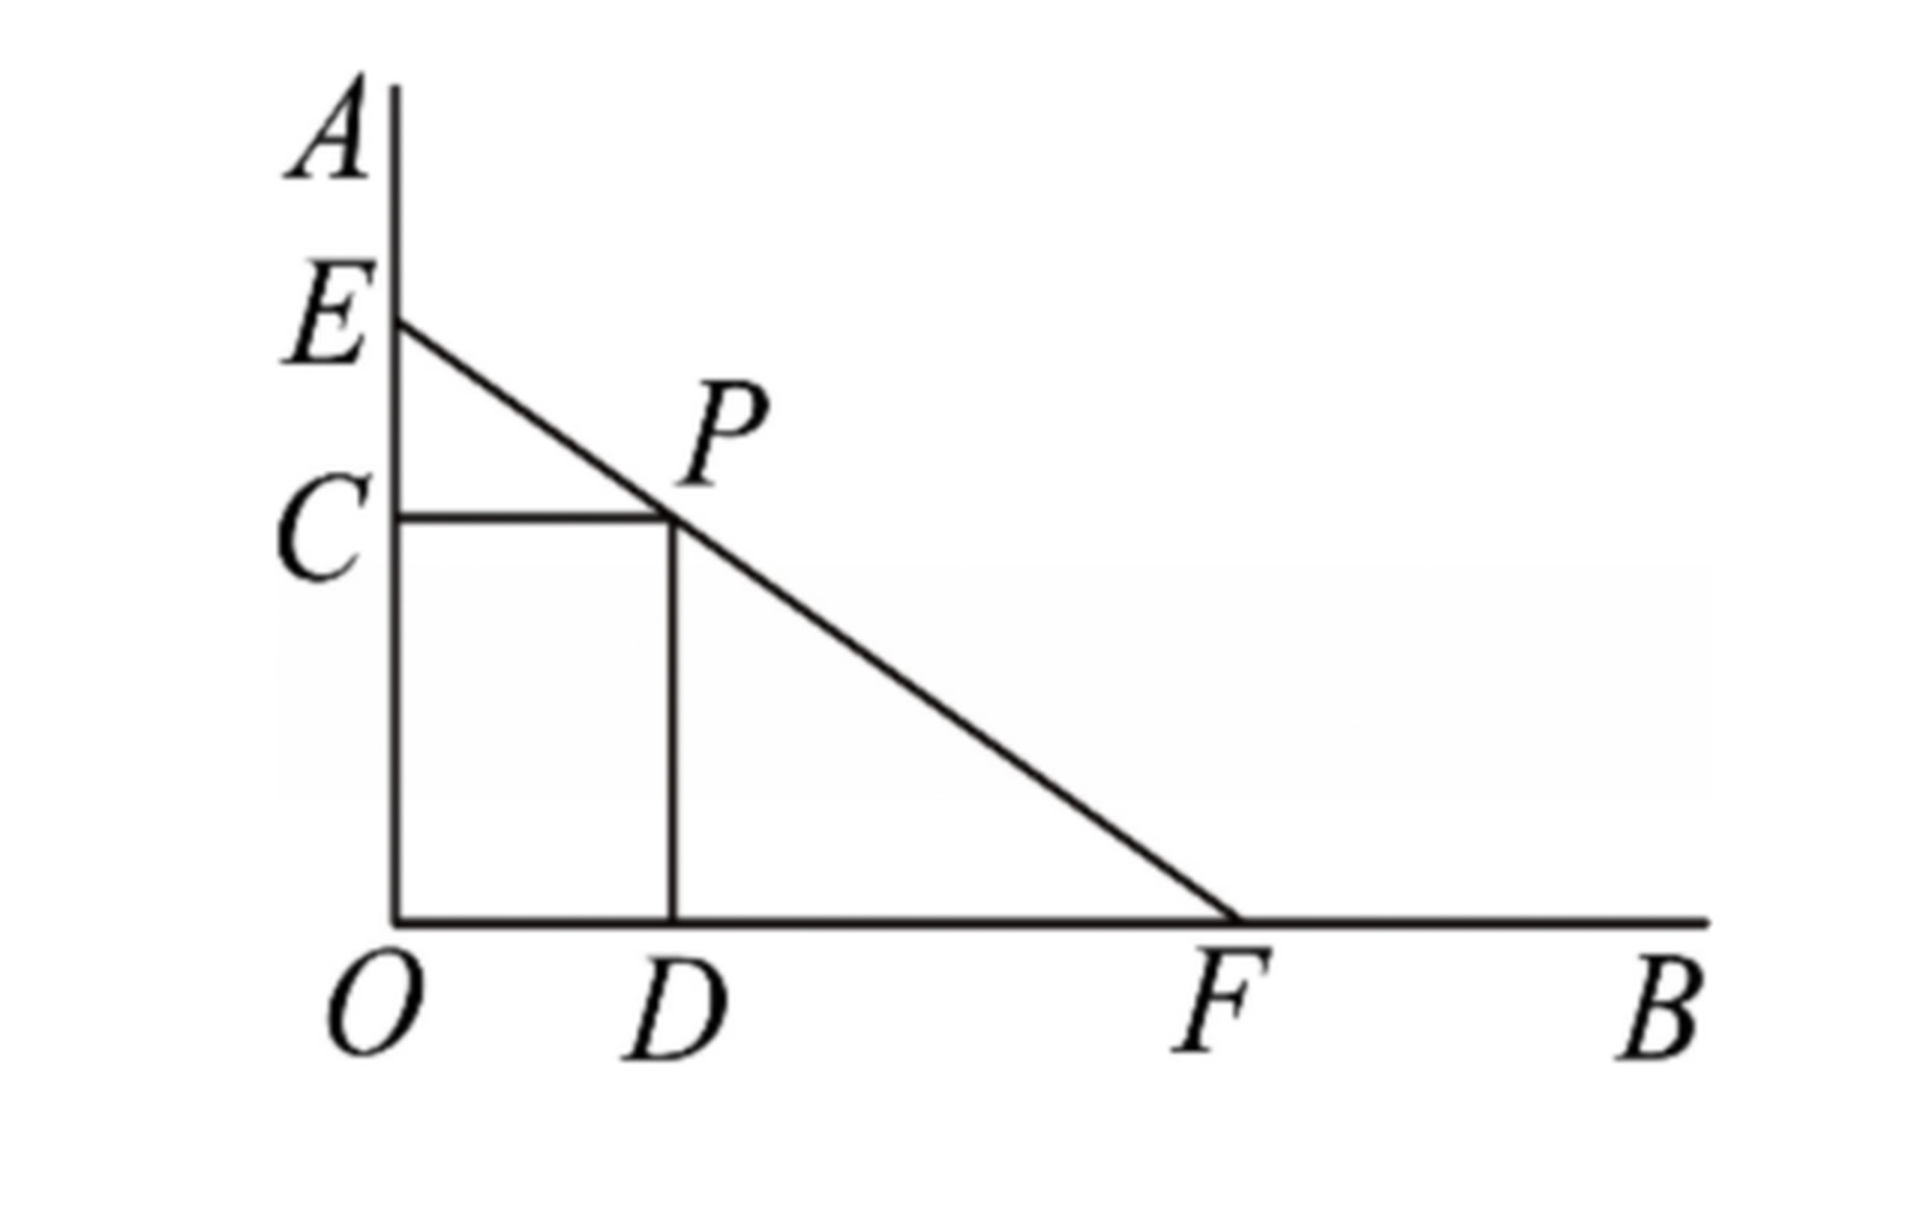
\includegraphics[width=0.32\textwidth]{figures/gao132_q18.png}
\end{center}

\ifanswer
\solbegin
\step{(1) 由题意得 $x\leq60$，}
\step{$\triangle PCE\sim\triangle FDP$，所以 $\dfrac{EC}{CP}=\dfrac{PD}{DF}$，即 $\dfrac{x}{25}=\dfrac{40}{DF}$，得 $DF=\dfrac{1000}{x}$m，}
\step{所以 $OF=OD+DF=\left(25+\dfrac{1000}x\right)$m，}
\step{所以 $25+\dfrac{1000}x\leq100$，解得 $x\geq\dfrac{40}3$；}
\step{综上，$\dfrac{40}3\leq x\leq60$；}
\step{(2) 由 $OE=OC+CE=(40+x)$m，}
\step{所以 $S=\dfrac12 OF\cdot OE=\dfrac12\left(25+\dfrac{1000}x\right)(40+x)$}
\step{$=\dfrac12\left(1000+25x+\dfrac{40000}x+1000\right)$m$^2$，}
\step{由基本不等式得 $S\geq\dfrac12\left(2000+2\sqrt{25x\cdot\dfrac{40000}x}\right)=2000$m$^2$，}
\step{当且仅当 $25x=\dfrac{40000}x$，即 $x=40$ 时取等号，}
\step{故 $EC=40$m 时，$S$ 取得最小值，为 $2000$m$^2$.}
\solend
\fi

\item 已知 $a>0$，$b>0$，请选择适当的方法证明.

(1) 若 $a\ne b$，证明：$a^3+b^3>a^2b+ab^2$；

(2) 若 $ab=1$，证明：$a^2+a<2$ 与 $b^2+b<2$ 不能同时成立.

\ifanswer
\solbegin
\step{(1) 因为 $a>0$，$b>0$，$a\ne b$，}
\step{所以 $a^3+b^3-a^2b-ab^2=a^2(a-b)+b^2(b-a)$}
\step{$=(a^2-b^2)(a-b)=(a-b)^2(a+b)>0$，所以 $a^3+b^3>a^2b+ab^2$.}
\step{(2) 假设 $a^2+a<2$ 与 $b^2+b<2$ 同时成立，所以 $-2<a<1,-2<b<1$，}
\step{又因为 $a>0,b>0$，所以 $0<a<1,0<b<1$，}
\step{所以 $0<ab<1$，这与 $ab=1$ 矛盾，}
\step{故 $a^2+a<2$ 与 $b^2+b<2$ 不可能同时成立.}
\solend
\fi

\item 若设 $M(a,n)=\lvert ax-1\rvert+\lvert ax-2\rvert+\cdots+\lvert ax-n\rvert$ 为曼哈顿扩张距离，它由 $n$ 个绝对值之和组成，其中 $n$ 为正整数.

(1) 若 $M(2,1)\leq5$，求 $x$ 的取值范围；

(2) 若 $k\leq M(2,2)$ 对一切实数 $x$ 恒成立，求实数 $k$ 的取值范围；

(3) $M(2,6)$ 是否存在最小值？若存在，求出该最小值与此时实数 $x$ 的取值范围；若不存在，说明理由.

\ifanswer
\solbegin
\step{(1) $M(2,1)=\lvert2x-1\rvert\leq5$，则不等式可化为 $-5\leq2x-1\leq5$，解得 $-2\leq x\leq3$，}
\step{所以 $x$ 的取值范围为 $[-2,3]$.}
\step{(2) 因为 $k\leq M(2,2)=\lvert2x-1\rvert+\lvert2x-2\rvert$ 对一切实数 $x$ 恒成立，}
\step{又 $\lvert2x-1\rvert+\lvert2x-2\rvert\geq\lvert(2x-1)-(2x-2)\rvert=1$，}
\step{当且仅当 $(2x-1)(2x-2)\leq0$，即 $\dfrac12\leq x\leq1$ 时取等号，}
\step{故 $k\leq1$，所以实数 $k$ 的取值范围为 $(-\infty,1]$.}
\step{(3) $M(2,6)=\lvert2x-1\rvert+\lvert2x-2\rvert+\lvert2x-3\rvert+\lvert2x-4\rvert+\lvert2x-5\rvert+\lvert2x-6\rvert$}
\step{$=2\left(\left\lvert x-\dfrac12\right\rvert+\lvert x-1\rvert+\left\lvert x-\dfrac32\right\rvert+\lvert x-2\rvert+\left\lvert x-\dfrac52\right\rvert+\lvert x-3\rvert\right)$，}
\step{其中 $\left\lvert x-\dfrac12\right\rvert+\lvert x-1\rvert+\left\lvert x-\dfrac32\right\rvert+\lvert x-2\rvert+\left\lvert x-\dfrac52\right\rvert+\lvert x-3\rvert$ 的几何意义为}
\step{在数轴上一点 $x$ 到 $\dfrac12,1,\dfrac32,2,\dfrac52,3$ 的距离之和，}
\step{要想距离之和最小，其中 $x\in\left[\dfrac12,3\right]$ 时，$\left\lvert x-\dfrac12\right\rvert+\lvert x-3\rvert$ 取得最小值，}
\step{当 $x\in\left[1,\dfrac52\right]$ 时，$\lvert x-1\rvert+\left\lvert x-\dfrac52\right\rvert$ 取得最小值，}
\step{当 $x\in\left[\dfrac32,2\right]$ 时，$\left\lvert x-\dfrac32\right\rvert+\lvert x-2\rvert$ 取得最小值，}
\step{综上，当 $x\in\left[\dfrac32,2\right]$ 时，$\left\lvert x-\dfrac12\right\rvert+\lvert x-1\rvert+\left\lvert x-\dfrac32\right\rvert+\lvert x-2\rvert+\left\lvert x-\dfrac52\right\rvert+\lvert x-3\rvert$}
\step{取得最小值，最小值为 $3-\dfrac12+\dfrac52-1+2-\dfrac32=\dfrac92$，}
\step{故 $M(2,6)=2\left(\left\lvert x-\dfrac12\right\rvert+\lvert x-1\rvert+\left\lvert x-\dfrac32\right\rvert+\lvert x-2\rvert+\left\lvert x-\dfrac52\right\rvert+\lvert x-3\rvert\right)$ 的}
\step{最小值为 $9$.}
\solend
\fi

\item 已知集合 $A=\{a_1,a_2,\cdots,a_n\}(0\leq a_1<a_2<\cdots<a_n,n\in\N,n\geq3)$ 具有性质 $Q$：对任意 $i,j(1\leq i\leq j\leq n)$，$a_i+a_j$ 与 $a_j-a_i$ 至少有一个属于集合 $A$；

(1) 判断集合 $M=\{0,2,4\}$ 与 $N=\{2,3,4\}$ 是否具有性质 $Q$，并说明理由；

(2) 已知 $A=\{a_1,a_2,a_3\}$ 具有性质 $Q$，当 $a_2=2026$ 时，求集合 $A$；

(3) 已知 $B=\{b_1,b_2,\cdots,b_{2026}\}$ 具有性质 $Q$，求 $\dfrac{b_1+b_2+\cdots+b_{2026}}{b_{2026}}$ 的值；

\ifanswer
\solbegin
\step{(1) 集合 $M=\{0,2,4\}$ 中，}
\step{因为 $0+2\in M,0+4\in M,4-2\in M,0\pm0=0\in M$，}
\step{$2+2=4\in M,2-2=0\in M,4-4=0\in M$，所以集合 $M$ 具有性质 $Q$；}
\step{集合 $N=\{2,3,4\}$ 中，因为 $3+3=6\notin N,3-3=0\notin N$，}
\step{所以集合 $N$ 不具有性质 $Q$.}
\step{(2) 因为 $a_1<a_2<a_3$，且 $A=\{a_1,a_2,a_3\}$ 具有性质 $Q$，}
\step{所以 $a_3+a_3\notin A,a_3-a_3=0\in A$，则 $a_1=0$，}
\step{又因为 $a_2+a_3>a_3$，所以 $a_2+a_3\notin A$，则 $a_3-a_2\in A$，}
\step{由集合的互异性得 $a_3-a_2=a_2$，而 $a_2=2026$，所以 $a_3=4052$，}
\step{故 $A=\{0,2026,4052\}$；}
\step{(3) 先证明一般结论：$A=\{a_1,a_2,\cdots,a_n\}(0\leq a_1<a_2<\cdots<a_n,n\in\N,n\geq3)$}
\step{具有性质 $Q$，则 $a_1+a_2+a_3+\cdots+a_n=\dfrac n2 a_n$.}
\step{因为 $A=\{a_1,a_2,\cdots,a_n\}(0\leq a_1<a_2<\cdots<a_n,n\in\N,n\geq3)$ 具有性质 $Q$，}
\step{所以 $a_n+a_n\notin A$，则 $a_n-a_n=0\in A$，则 $a_1=0$.}
\step{又因为 $0\leq a_1<a_2<\cdots<a_n$，所以 $0\leq a_n-a_n<a_n-a_{n-1}<\cdots<a_n-a_1$，}
\step{又因为 $a_n+a_{n-i}>a_n(i=1,2,\cdots,n-1)$，所以 $a_n+a_{n-i}\notin A$，}
\step{则 $a_n-a_{n-i}\in A$，}
\step{所以 $a_1=a_n-a_n,a_2=a_n-a_{n-1},a_3=a_n-a_{n-2},\cdots,a_n=a_n-a_1$.}
\step{所以 $a_1+a_2+a_3+\cdots+a_n$}
\step{$=(a_n-a_n)+(a_n-a_{n-1})+(a_n-a_{n-2})+\cdots+(a_n-a_1)$，}
\step{即 $a_1+a_2+a_3+\cdots+a_n=\dfrac n2 a_n$，}
\step{所以 $B=\{b_1,b_2,\cdots,b_{2026}\}$ 具有性质 $Q$，则 $b_1+b_2+\cdots+b_{2026}=\dfrac{2026}{2}b_{2026}$，}
\step{所以 $\dfrac{b_1+b_2+\cdots+b_{2026}}{b_{2026}}=\dfrac{2026}{2}=1013$.}
\solend
\fi

\end{enumerate}

% 行数复核：逐题数 \step 条数，合计 144 条（Q3：4；Q4：1；Q5：4；Q6：2；Q7：9；Q8：2；
% Q9：3；Q10：6；Q11：9；Q12：9；Q13：0；Q14：9；Q15：4；Q16：19；Q17：5；Q18：11；
% Q19：7；Q20：17；Q21：23），与原卷印刷行逐题相等（cases 块作一个印刷行计）。
% 第 13 题只印括号内答案、提 \ans{}，不计入 \step 账；第 14—16 题答案在解析末句，
% 括号内留空、不另提 \ans{}。

\end{document}
"
%
% 原始材料：微信公众号"魔都数学加油站"文章，作者破晓，2026-11-14 19:00 发布；
% 连载"27学年高一132"，原文标题"27学年高一132——2026-2027年上海市川沙中学高一上期中"；
% 原文链接：https://mp.weixin.qq.com/s/VBG01CrUNMIYWWHhSfz8JQ。
% 正文为 11 张 PNG 页（01、04、06、07、09、11 为 2560x3620，02、03、05、08、10 为 4762x6735），
% 题目下印有【解析】，为讲评版。题目、解析均据原图转录；
% 卷面粉红色水印"魔都数学加油站"及公众号页脚未录入。全卷 2 幅插图：第 14 题四幅坐标图选项、
% 第 18 题矩形 OCPD 与小路 EF 示意图，均取原卷 04／07 页截图去水印。
%
% 卷首标题：原卷印作"2026-2027 年川沙中学高一上期中"（公众号标题中的"上海市"
% 卷面标题行没有，本稿照卷面），年份区间按全稿惯例排 en dash；原卷未印副标题，
% 本卷为期中卷、跨集合与常用逻辑用语／不等式／函数三章，按题目内容标为
% "集合与常用逻辑用语、不等式、函数"（与 125／126／128／129／131 同期中卷口径相同）：
% 集合与逻辑见 Q5、Q6、Q17、Q21，不等式见 Q3、Q4、Q9、Q10、Q12、Q13、Q15、Q16、Q19，
% 函数（幂函数、指数／对数、基本不等式应用）见 Q7、Q8、Q11、Q14、Q18、Q20。
%
% 题号体例：本卷共 19 题——一、填空题 3—12（10 题）、二、选择题 13—16（4 题）、
% 三、解答题 17—21（5 题）。三节分别 \setcounter{enumi}{2}／{12}／{16}。
%
% 与原卷的排版差异：
%   ① 原文从第 3 题起，本稿保留原题号（见上"题号体例"）；
%   ② 原卷每题下直接印【解析】，本稿按全稿惯例置于答案版；第 13 题答案 D 印在题干
%      括号内、无独立答案段，按 高一37／52／53／55／63／64／128／131 成例括号留空、
%      另提 \ans{$D$}；第 14—16 题答案在解析末句"故选 …"，括号内留空、不另提 \ans{}；
%   ③ 原卷未印副标题，本稿按"知识模块"口径补出；
%   ④ 原卷填空横线按全稿惯例排为 \blankline[4.4em]；选择题括号排 \mbox{（\quad）}、
%      选项段前按惯例加 \keepwithprev；解答题不留作答区（原卷为讲评版，与 109—131 同）；
%   ⑤ 原卷数集排斜体 $R^+$／$R$／$Z$／$N$，按全稿惯例改 \R^+／\R／\Z／\N；
%      绝对值排 \lvert…\rvert，集合描述竖线排 \mid；不等号按全稿惯例排 \leqslant／\geqslant；
%      补集照原卷上划线排 \overline{B}；
%   ⑥ 子题标号 (1)(2)(3) 原卷用半角括号，照录；第 14 题四幅坐标图选项按原卷 2×2 排布
%      合并裁为一张 \includegraphics（未用 TikZ 重绘，以保证与原卷一致），题前加
%      \needvspace{9cm} 守卫；第 18 题图取 07 页截图，题前按惯例加 \needvspace{7cm} 守卫
%      （照 高一120／127／129／131 成例），两者守卫都放在 \item 之前；
%   ⑦ 原卷 Q7 解析跨 01—02 页、Q10 解析跨 02—03 页、Q12 解析跨 03—04 页、
%      Q14 解析跨 04—05 页、Q16 解析在 06 页、Q18 解析跨 07—08 页、
%      Q20 解析跨 08—09 页、Q21 解析跨 10—11 页，本稿按题合并连续排版；
%      末页第 11 页为 Q21 (3) 解析的续尾，按实际印刷行单列。
%
% 判别式字形：第 10 题 $\triangle=4(a-1)^2+16(a-1)<0$、第 11 题
%   $\triangle=4(m-2)^2-4(m^2-3m+3)=-4m+4>0$ 两处原卷均排 $\triangle$（等边、扁），
%   逐处放大核对、字形一致，照录 \triangle；与 高一129／131 同题排 $\Delta$（等腰、高）不同。
%   全卷 \triangle 兼作第 18 题「$\triangle PCE\sim\triangle FDP$」「$\triangle OEF$」的几何
%   三角形记号，全卷未出现 \Delta。
%
% 子集符号：第 5 题解析 $B\subseteq A$、第 17 题 (2) 解析 $A\subseteq B$ 均印带下划线，
%   照录 \subseteq；全卷未出现单线 \subset。
%
% 原卷存疑照录：
%   第 9 题题干作"充分非必要条件"、解析作"充分不必要条件"，措辞不同，照录；
%   第 10 题解析"当 $a-1=0$ 时，$-4\geq0$，不等式不成立，$a=1$ 满足题意"照录；
%   第 11 题解析"所以 $2(m-1)+\dfrac1{m-1}\leq-2\sqrt2$"由上一行 $2(1-m)+\dfrac1{1-m}\geq2\sqrt2$
%     直接变号得到，照录；
%   第 12 题解析"由 $x\in Z$，$-7<-2\sqrt{10}<-6$"与"即 $k^2+7k+10\leq0$，解得 $-5\leq k\leq-2$"照录；
%   第 16 题解析"令 $52\times(930+a)=-52$，解得 $a=-931$"（按式应为 $a=-931$ 之外的解）照录；
%   第 19 题 (2) 解析"所以 $-2<a<1,-2<b<1$"数学式内半角逗号，照录；
%   第 20 题 (3) 解析"最小值为 $3-\dfrac12+\dfrac52-1+2-\dfrac32=\dfrac92$"与
%     "故 $M(2,6)=\dots$ 的最小值为 9"两处结论并列，照录；
%   第 21 题 (1) 解析"$0+2\in M,0+4\in M,4-2\in M,0\pm0=0\in M$"、
%     "$2+2=4\in M,2-2=0\in M,4-4=0\in M$"、(3) 各连写等式内半角逗号，照录；
%   第 21 题 (3) 解析"即 $a_1+a_2+a_3+\cdots+a_n=\dfrac n2 a_n$，"句末用半角逗号，照录。
%
% 行数复核：见文末"行数复核"注（逐题 \step 条数与原卷印刷行逐题相等，cases 块作一个印刷行计）。
%   第 13 题只印括号内答案、提 \ans{}，不计入 \step 账；第 14—16 题答案在解析末句，
%   括号内留空、不另提 \ans{}。
%
\documentclass[a4paper,11pt]{article}
\usepackage{common}

\begin{document}

\examtitlest[3]{2026--2027 年川沙中学高一上期中}{集合与常用逻辑用语、不等式、函数}

\bigsec{一、填空题}

\begin{enumerate}
\setcounter{enumi}{2}

\item 已知 $a$、$b\in\R^+$ 且 $ab=2$，则 $a+2b$ 的最小值为\blankline[4.4em].

\ifanswer
\solbegin
\step{因为 $a\in\R^+$，$b\in\R^+$ 且 $ab=2$，}
\step{由基本不等式得 $a+2b\geq2\sqrt{a\cdot2b}=2\sqrt{2ab}=2\sqrt4=4$.}
\step{等号当且仅当 $a=2b$ 时成立，结合 $ab=2$ 解得 $b=1$，$a=2$，}
\step{所以 $a+2b$ 的最小值为 $4$.}
\solend
\fi

\item 如果幂函数 $f(x)=(m^2-3m-3)x^{m^2+m-3}$ 在 $(0,+\infty)$ 上是增函数，则实数 $m=$\blankline[4.4em].

\ifanswer
\solbegin
\step{由已知得 $\begin{cases}m^2-3m-3=1\\m^2+m-3>0\end{cases}$，所以 $m=4$.}
\solend
\fi

\item 已知集合 $A=\{1,2\}$，集合 $B=\{x\mid ax=6\}$，若 $A\cup B=A$，则 $a$ 的所有取值构成的集合为\blankline[4.4em].

\ifanswer
\solbegin
\step{因为 $A\cup B=A$，所以 $B\subseteq A$，}
\step{当 $a=0$ 时，$B=\varnothing$，满足 $B\subseteq A$；}
\step{当 $a\ne0$ 时，$B=\left\{\dfrac6a\right\}$，则 $\dfrac6a=1$ 或 $\dfrac6a=2$，解得 $a=6$ 或 $a=3$，}
\step{综上所述，$a$ 的所有取值构成的集合为 $\{0,3,6\}$.}
\solend
\fi

\item 设全集为 $\R$，$A=\{y\mid y=-x^2+2x+1\}$，$B=\{x\mid y=\ln(x-1)\}$，则 $A\cap B=$\blankline[4.4em].

\ifanswer
\solbegin
\step{$A=\{y\mid y=-x^2+2x+1\}=\{y\mid y=-(x-1)^2+2\}=\{y\mid y\leq2\}$，}
\step{$B=\{x\mid y=\ln(x-1)\}=\{x\mid x>1\}$，则 $A\cap B=(1,2]$.}
\solend
\fi

\item 已知 $x\in\R$，则方程 $\lvert 6-x\rvert+\lvert 6x-3\rvert=\lvert 5x+3\rvert$ 的解集为\blankline[4.4em].

\ifanswer
\solbegin
\step{当 $x<-\dfrac35$ 时，$6-x>0$，$6x-3<0$，$5x+3<0$，}
\step{原方程为 $6-x-6x+3=-5x-3$，解得 $x=6$，不满足 $x<-\dfrac35$；}
\step{当 $-\dfrac35\leq x\leq\dfrac12$ 时，$5x+3\geq0$，$6x-3<0$，$6-x>0$，}
\step{原方程为 $6-x+3-6x=5x+3$，解得 $x=\dfrac12$；}
\step{当 $\dfrac12<x\leq6$ 时，$5x+3>0$，$6x-3>0$，$6-x\geq0$，}
\step{原方程为 $6-x+6x-3=5x+3$，即 $0=0$，恒成立，所以 $\dfrac12<x\leq6$；}
\step{当 $x>6$ 时，$5x+3\geq0$，$6x-3>0$，$6-x<0$，}
\step{原方程为 $x-6+6x-3=5x+3$，解得 $x=6$，不满足 $x>6$；}
\step{综上 $\dfrac12\leq x\leq6$，所以原方程的解集为 $\left\{x\mid\dfrac12\leq x\leq6\right\}$.}
\solend
\fi

\item 已知 $\log_2 3=a,2^b=7$，用 $a,b$ 表示 $\log_{42}56$ 为\blankline[4.4em].

\ifanswer
\solbegin
\step{$\log_{42}56=\dfrac{\log_2 56}{\log_2 42}=\dfrac{\log_2(7\times8)}{\log_2(6\times7)}=\dfrac{\log_2 7+\log_2 8}{\log_2 6+\log_2 7}$}
\step{$=\dfrac{\log_2 7+\log_2 2^3}{\log_2 2+\log_2 3+\log_2 7}=\dfrac{b+3}{1+a+b}$.}
\solend
\fi

\item 已知 $\dfrac13<x<\dfrac12$ 是不等式 $\lvert x-m\rvert<1$ 成立的充分非必要条件，则 $m$ 的取值范围是\blankline[4.4em].

\ifanswer
\solbegin
\step{因为 $\lvert x-m\rvert<1$，所以 $-1<x-m<1$，所以 $m-1<x<m+1$，}
\step{所以 $m-1<x<m+1$ 成立的充分不必要条件是 $\dfrac13<x<\dfrac12$，}
\step{所以 $\begin{cases}m-1\leq\dfrac13\\m+1\geq\dfrac12\end{cases}$，解得 $-\dfrac12\leq m\leq\dfrac43$，故 $m$ 的取值范围是 $\left[-\dfrac12,\dfrac43\right]$.}
\solend
\fi

\item 若关于 $x$ 的不等式 $(a-1)x^2+2(a-1)x-4\geq0$ 的解集为空集，则 $a$ 的取值范围是\blankline[4.4em].

\ifanswer
\solbegin
\step{关于 $x$ 的不等式 $(a-1)x^2+2(a-1)x-4\geq0$ 的解集为 $\varnothing$，}
\step{当 $a-1=0$ 时，$-4\geq0$，不等式不成立，$a=1$ 满足题意；}
\step{当 $a-1>0$ 时，$a>1$，不等式的解集不为空集，不满足题意；}
\step{当 $a-1<0$ 时，$a<1$，当 $\triangle=4(a-1)^2+16(a-1)<0$ 时，即 $(a-1)(a+3)<0$，}
\step{解得 $-3<a<1$，满足题意；}
\step{综上，实数 $a$ 的取值范围是 $\{a\mid-3<a\leq1\}$.}
\solend
\fi

\item 已知关于 $x$ 的方程 $x^2+2(m-2)x+m^2-3m+3=0$ 有两个不相等的实数根 $x_1$、$x_2$，则 $\dfrac{mx_1}{x_1-1}+\dfrac{mx_2}{x_2-1}-\dfrac{2}{x_1+x_2-2}$ 的最大值为\blankline[4.4em].

\ifanswer
\solbegin
\step{关于 $x$ 的方程 $x^2+2(m-2)x+m^2-3m+3=0$ 有两个不相等的实数根 $x_1$、$x_2$，}
\step{则 $\triangle=4(m-2)^2-4(m^2-3m+3)=-4m+4>0$，得 $m<1$，}
\step{且 $x_1+x_2=-2(m-2)$，$x_1x_2=m^2-3m+3$，}
\step{$\dfrac{mx_1}{x_1-1}+\dfrac{mx_2}{x_2-1}-\dfrac{2}{x_1+x_2-2}=\dfrac{m[2x_1x_2-(x_1+x_2)]}{x_1x_2-(x_1+x_2)+1}+\dfrac1{m-1}$}
\step{$=\dfrac{2m(m-1)^2}{m^2-m}+\dfrac1{m-1}=2(m-1)+\dfrac1{m-1}$，}
\step{又因为 $m<1$，所以 $m-1<0$，则 $1-m>0$，}
\step{所以 $2(1-m)+\dfrac1{1-m}\geq2\sqrt{2(1-m)\cdot\dfrac1{1-m}}=2\sqrt2$，}
\step{当且仅当 $2(1-m)=\dfrac1{1-m}$ 时，即 $m=1-\dfrac{\sqrt2}2$ 时取等号，}
\step{所以 $2(m-1)+\dfrac1{m-1}\leq-2\sqrt2$，即 $\dfrac{mx_1}{x_1-1}+\dfrac{mx_2}{x_2-1}-\dfrac2{x_1+x_2-2}$ 的最大值为 $-2\sqrt2$.}
\solend
\fi

\item 若使集合 $A=\{x\mid(kx-k^2-10)(x-1)>0,x\in\Z\}$ 中的元素个数最少，则实数 $k$ 的取值范围是\blankline[4.4em].

\ifanswer
\solbegin
\step{由题意集合 $A=\{x\mid(kx-k^2-10)(x-1)>0,\ x\in\Z\}$，}
\step{$k=0$ 时，不等式解得 $x<1$，有无数个整数解；}
\step{$k\ne0$ 时，则不等式变形为 $k\left(x-k-\dfrac{10}k\right)(x-1)>0$，}
\step{当 $k>0$ 时，$k+\dfrac{10}k\geq2\sqrt{10}$，仅当 $k=\sqrt{10}$ 时等号成立，}
\step{此时不等式解得 $x>k+\dfrac{10}k$ 或 $x<1$，有无数个整数解；}
\step{当 $k<0$ 时，$k+\dfrac{10}k=-\left[(-k)+\left(-\dfrac{10}k\right)\right]\leq-2\sqrt{10}$，仅当 $k=-\sqrt{10}$ 时等号成立，}
\step{此时不等式解得 $k+\dfrac{10}k<x<1$，}
\step{由 $x\in\Z$，$-7<-2\sqrt{10}<-6$，要使集合 $A$ 中的元素最少，则 $k+\dfrac{10}k\geq-7$，}
\step{即 $k^2+7k+10\leq0$，解得 $-5\leq k\leq-2$，故实数 $k$ 的取值范围是 $[-5,-2]$.}
\solend
\fi

\end{enumerate}

\bigsec{二、选择题}

\begin{enumerate}
\setcounter{enumi}{12}

\item 下列说法正确的是\mbox{（\quad）}

\keepwithprev
A. 若 $a>b$，则 $\dfrac1a<\dfrac1b$\qquad\qquad B. 若 $a>b$，$c>d$，则 $ac>bd$

C. 若 $a>b$，则 $ac^2>bc^2$\qquad\qquad D. 若 $ac^2>bc^2$，则 $a>b$

\ifanswer
\ans{$D$}
\fi

% 第 14 题四幅坐标图选项是一整块，守卫放在 \item 之前
\needvspace{9cm}
\item 在同一坐标系内，函数 $y=x^a(a\ne0)$ 和 $y=ax-\dfrac1a$ 的图象可能是\mbox{（\quad）}

\keepwithprev
\begin{center}
% 四幅坐标图选项取原卷 04 页截图去粉色水印，按原卷 2×2 排布合并为一张
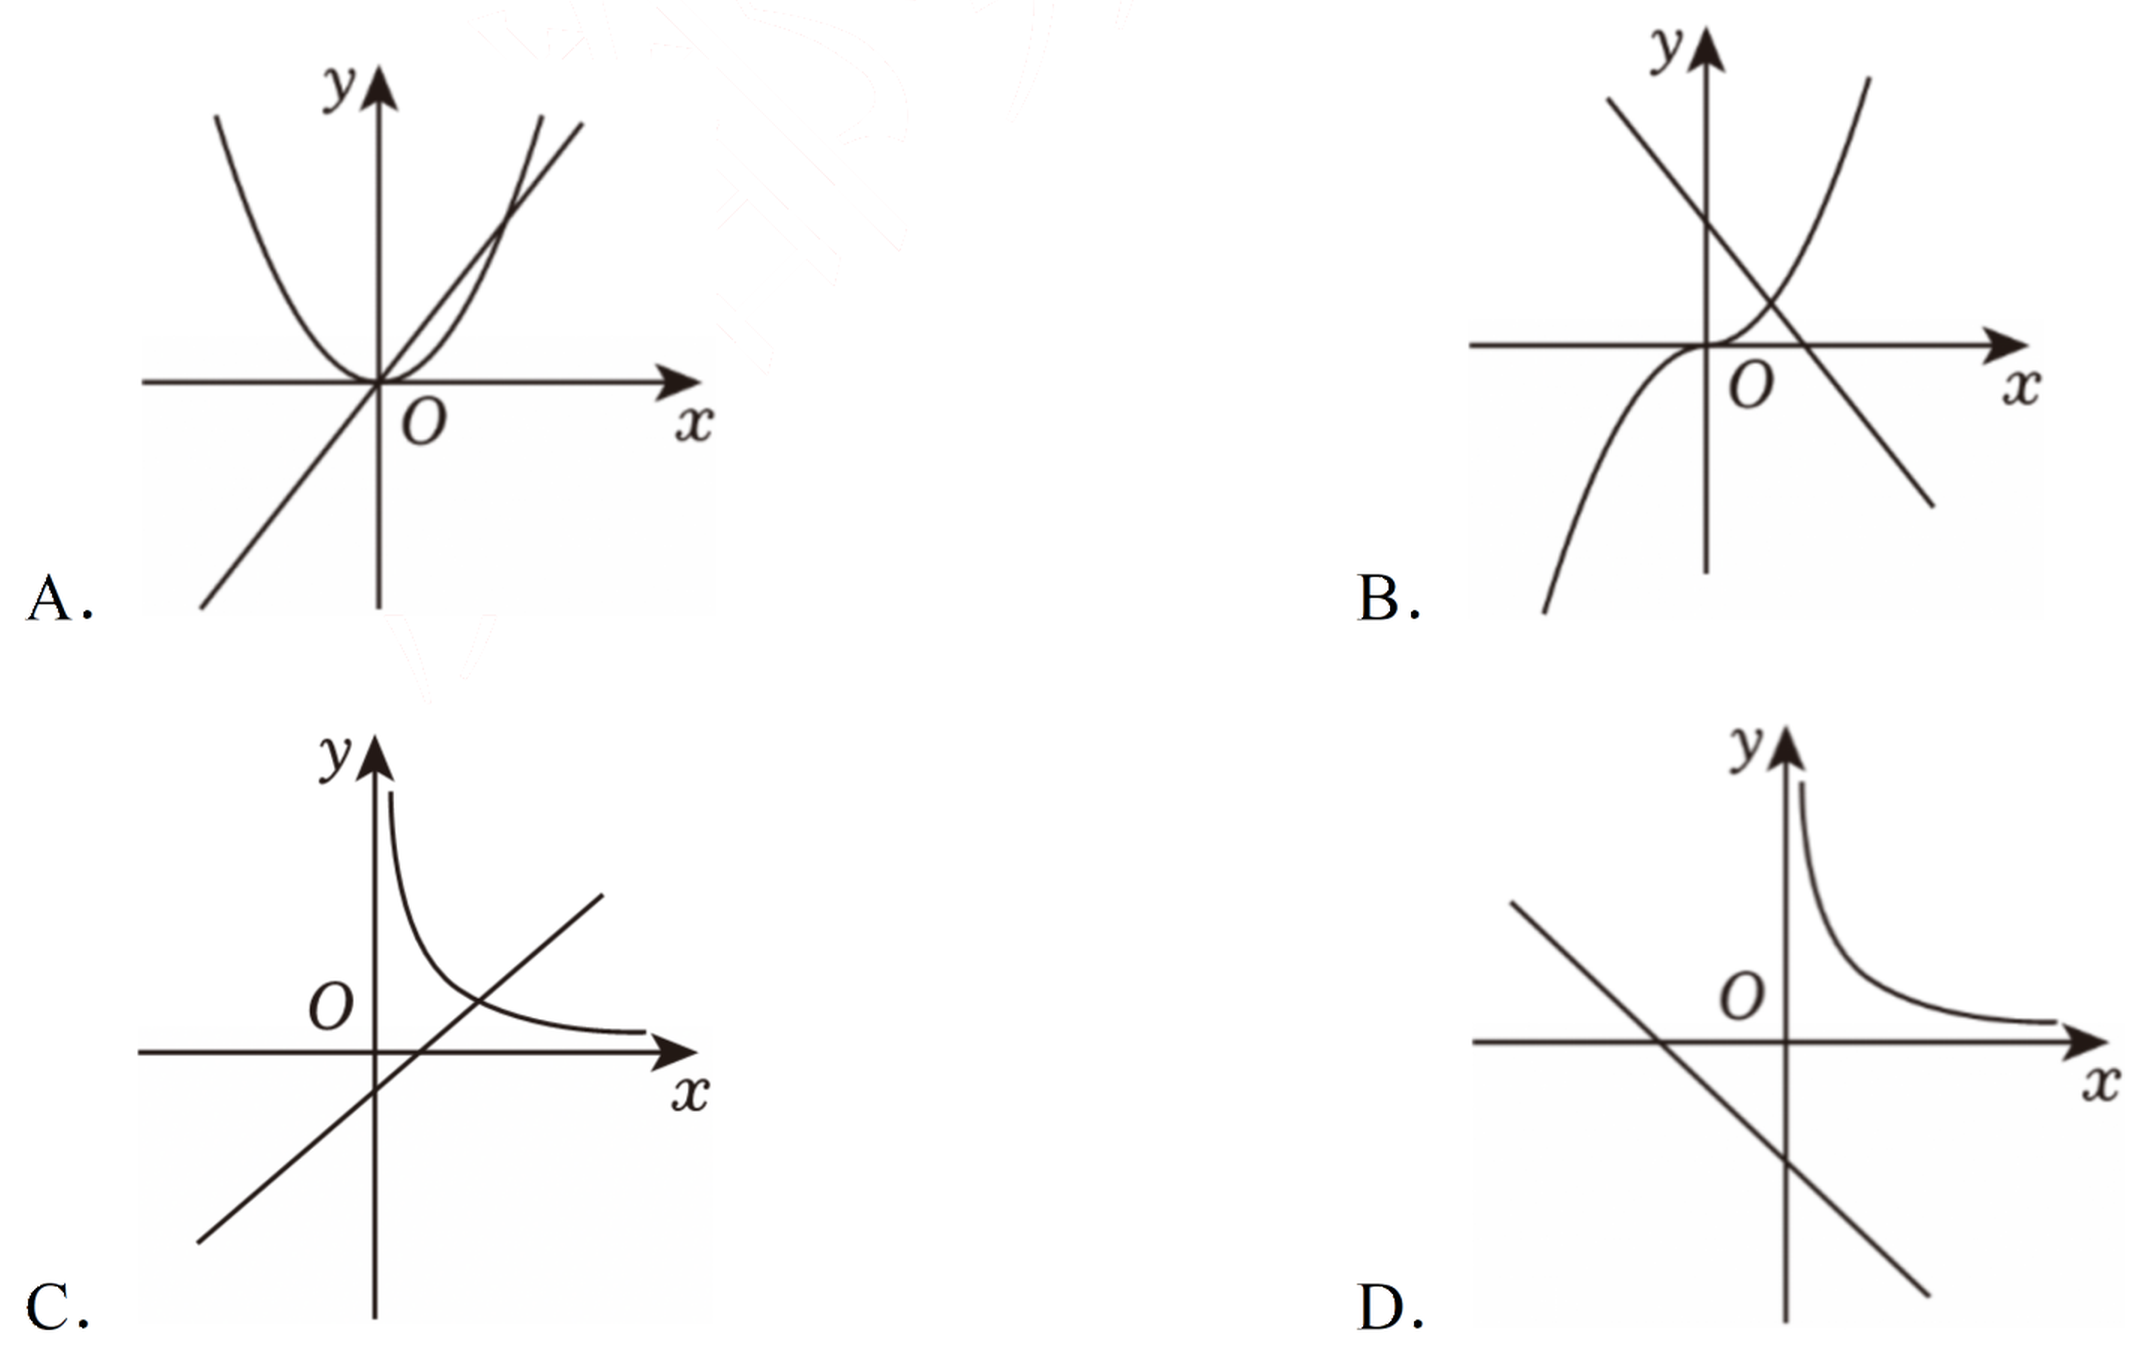
\includegraphics[width=0.80\textwidth]{figures/gao132_q14.png}
\end{center}

\ifanswer
\solbegin
\step{当 $a>0$ 时，$y=ax-\dfrac1a$ 严格增，当 $a<0$ 时，$y=ax-\dfrac1a$ 严格减，}
\step{对于 $A$，因为 $a\ne0$，所以直线 $y=ax-\dfrac1a$ 不过原点，故 $A$ 错误；}
\step{对于 $B$，由函数 $y=x^a(a\ne0)$ 的图象得 $a>1$，}
\step{由 $y=ax-\dfrac1a$ 的图象得 $a<0$，互相矛盾，故 $B$ 错误；}
\step{对于 $C$，由函数 $y=x^a(a\ne0)$ 的图象得 $a>1$，}
\step{由 $y=ax-\dfrac1a$ 的图象得 $a>0$ 且 $-\dfrac1a<0$，符合题意，故 $C$ 正确；}
\step{对于 $D$，由函数 $y=x^a(a\ne0)$ 的图象得 $a<0$，}
\step{由 $y=ax-\dfrac1a$ 的图象得 $a<0$ 且 $-\dfrac1a<0$，互相矛盾，故 $D$ 错误；}
\step{故选 $C$.}
\solend
\fi

\item 中国的 $5G$ 技术领先世界，在 $5G$ 技术中，最大数据传输速率 $C$ 取决于信道带宽 $W$，$C$ 与 $W$ 满足 $C=W\log_2\left(1+\dfrac SN\right)$，其中 $\dfrac SN$ 称为信噪比（单位：$dB$）. 若不改变带宽 $W$，初始信噪比 $\dfrac SN$ 为 $1000$，那么为了使 $C$ 增加 $30\%$，需要将信噪比 $\dfrac SN$ 从 $1000$ 提升至大约\mbox{（\quad）}

\keepwithprev
A. $5000$\qquad\qquad B. $6000$\qquad\qquad C. $7000$\qquad\qquad D. $8000$

\ifanswer
\solbegin
\step{由题意得 $\dfrac SN=1000$ 时，$C=W\log_2(1+1000)\approx W\log_2 1000$，}
\step{要使 $C$ 增加 $30\%$，则 $(1+30\%)C=W\log_2\left(1+\dfrac SN\right)$，即 $1.3C\approx W\log_2\dfrac SN$，}
\step{所以 $1.3\approx\log_{1000}\dfrac SN=\dfrac{\lg\frac SN}{\lg1000}$，所以 $\lg\dfrac SN=3.9$，所以 $\dfrac SN=10^{3.9}\approx8000$.}
\step{故选 $D$.}
\solend
\fi

\item 对于 $a\in\R$，设非空集合 $A=\left\{x\mid\dfrac{(x^2-930x+a)(x-52)}{x+a}=0\right\}$，记 $A$ 中的所有元素之和为 $S(a)$，所有元素之积为 $T(a)$，则下列说法中，不正确的是\mbox{（\quad）}

\keepwithprev
A. 存在实数 $a$，使得 $S(a)=930$

B. 存在实数 $a$，使得 $T(a)=517$

C. 不存在实数 $a$，使得 $T(a)=0$

D. 恰存在 $1$ 个实数 $a$，使得 $T(a)=-52$

\ifanswer
\solbegin
\step{由分式值为 $0$，得分子为 $0$ 且分母不为 $0$，}
\step{分子 $(x^2-930x+a)(x-52)=0$ 的根为 $x=52$}
\step{及方程 $x^2-930x+a=0$ 的两根 $x_1$，$x_2$，}
\step{由根与系数的关系得 $x_1+x_2=930$，$x_1\cdot x_2=a$，}
\step{分母限制 $x\ne-a$，需要剔除等于 $-a$ 的根，}
\step{选项 $A$，取 $a=-52$，$x=52$ 为增根舍去，集合 $A=\{x_1,x_2\}$，}
\step{元素之和 $S(a)=930$，故 $A$ 正确；}
\step{选项 $B$，当无增根时，$T(a)=52a$，令 $52a=517$，得 $a=\dfrac{517}{52}$，}
\step{验证无增根，存在这样的 $a$，故 $B$ 正确；}
\step{选项 $C$，若 $T(a)=0$，则 $0\in A$，代入分子得 $a=0$，}
\step{但 $a=0$ 时分母 $x\ne0$，$x=0$ 为增根，$0$ 不能属于集合 $A$，}
\step{故不存在 $a$ 使得 $T(a)=0$，故 $C$ 正确；}
\step{选项 $D$，当无增根时，令 $52a=-52$，得 $a=-1$；}
\step{当 $x=-a$ 是二次方程的根且不等于 $52$ 时，}
\step{令 $52\times(930+a)=-52$，解得 $a=-931$，验证符合条件；}
\step{当 $a=-52$ 时，$x=52$，舍去，}
\step{集合 $A=\{x_1,x_2\}$，$T(a)=a=-52$，得到两个满足条件的 $a$；}
\step{因此存在 $3$ 个满足条件的 $a$，故 $D$ 错误.}
\step{故选 $D$.}
\solend
\fi

\end{enumerate}

\bigsec{三、解答题}

\begin{enumerate}
\setcounter{enumi}{16}

\item 已知全集 $U=\R$，集合 $A=\left\{x\mid\dfrac{x}{x-3}<0\right\}$，$B=\{x\mid(x-a)(x+4-a)<0\}$.

(1) 当 $a=2$ 时，求 $\overline{B}$、$A\cap\overline{B}$；

(2) 若 $A\cap B=A$，求实数 $a$ 的取值范围.

\ifanswer
\solbegin
\step{(1) $\dfrac{x}{x-3}<0$，即 $x(x-3)<0$，解得 $A=\{x\mid0<x<3\}$，}
\step{当 $a=2$ 时，$B=\{x\mid(x-a)(x+4-a)<0\}=\{x\mid-2<x<2\}$，}
\step{则 $\overline{B}=\{x\mid x\leq-2$ 或 $x\geq2\}$，故 $A\cap\overline{B}=\{x\mid2\leq x<3\}$；}
\step{(2) $A\cap B=A$，则 $A\subseteq B$，故 $\begin{cases}a-4\leq0\\a\geq3\end{cases}$，解得 $3\leq a\leq4$，}
\step{故实数 $a$ 的取值范围是 $\{a\mid3\leq a\leq4\}$.}
\solend
\fi

% 第 18 题是"题干 + 图"约 7cm 的一整块，守卫放在 \item 之前
\needvspace{7cm}
\item 如图，$OA$、$OB$ 是两条长度足够长的互相垂直的笔直小路，矩形 $OCPD$ 的顶点 $C$、$D$ 分别在 $OA$、$OB$ 上，且该矩形区域内种满了荷花. 为了让观赏者有更好的观赏体验，现计划经过点 $P$ 修一条小路 $EF$，其中点 $E$ 在小路 $OA$ 上，点 $F$ 在小路 $OB$ 上，并在 $\triangle OEF$ 区域内种满荷花. 已知 $OD=25m$，$OC=40m$，且小路 $EF$ 要完全位于一个以 $O$ 为顶点的，边长为 $100$ m 的正方形内部（包括边界）. 记 $\triangle OEF$ 的面积为 $S$m$^2$.

(1) 设 $EC=x\cdot m$，试用 $x$ 表示 $OF$，并求 $x$ 的取值范围.

(2) 当 $EC$ 的长度为多少时，$S$ 取得最小值？最小值是多少？

\begin{center}
% 图取原卷 07 页截图去粉色水印，3× LANCZOS 放大
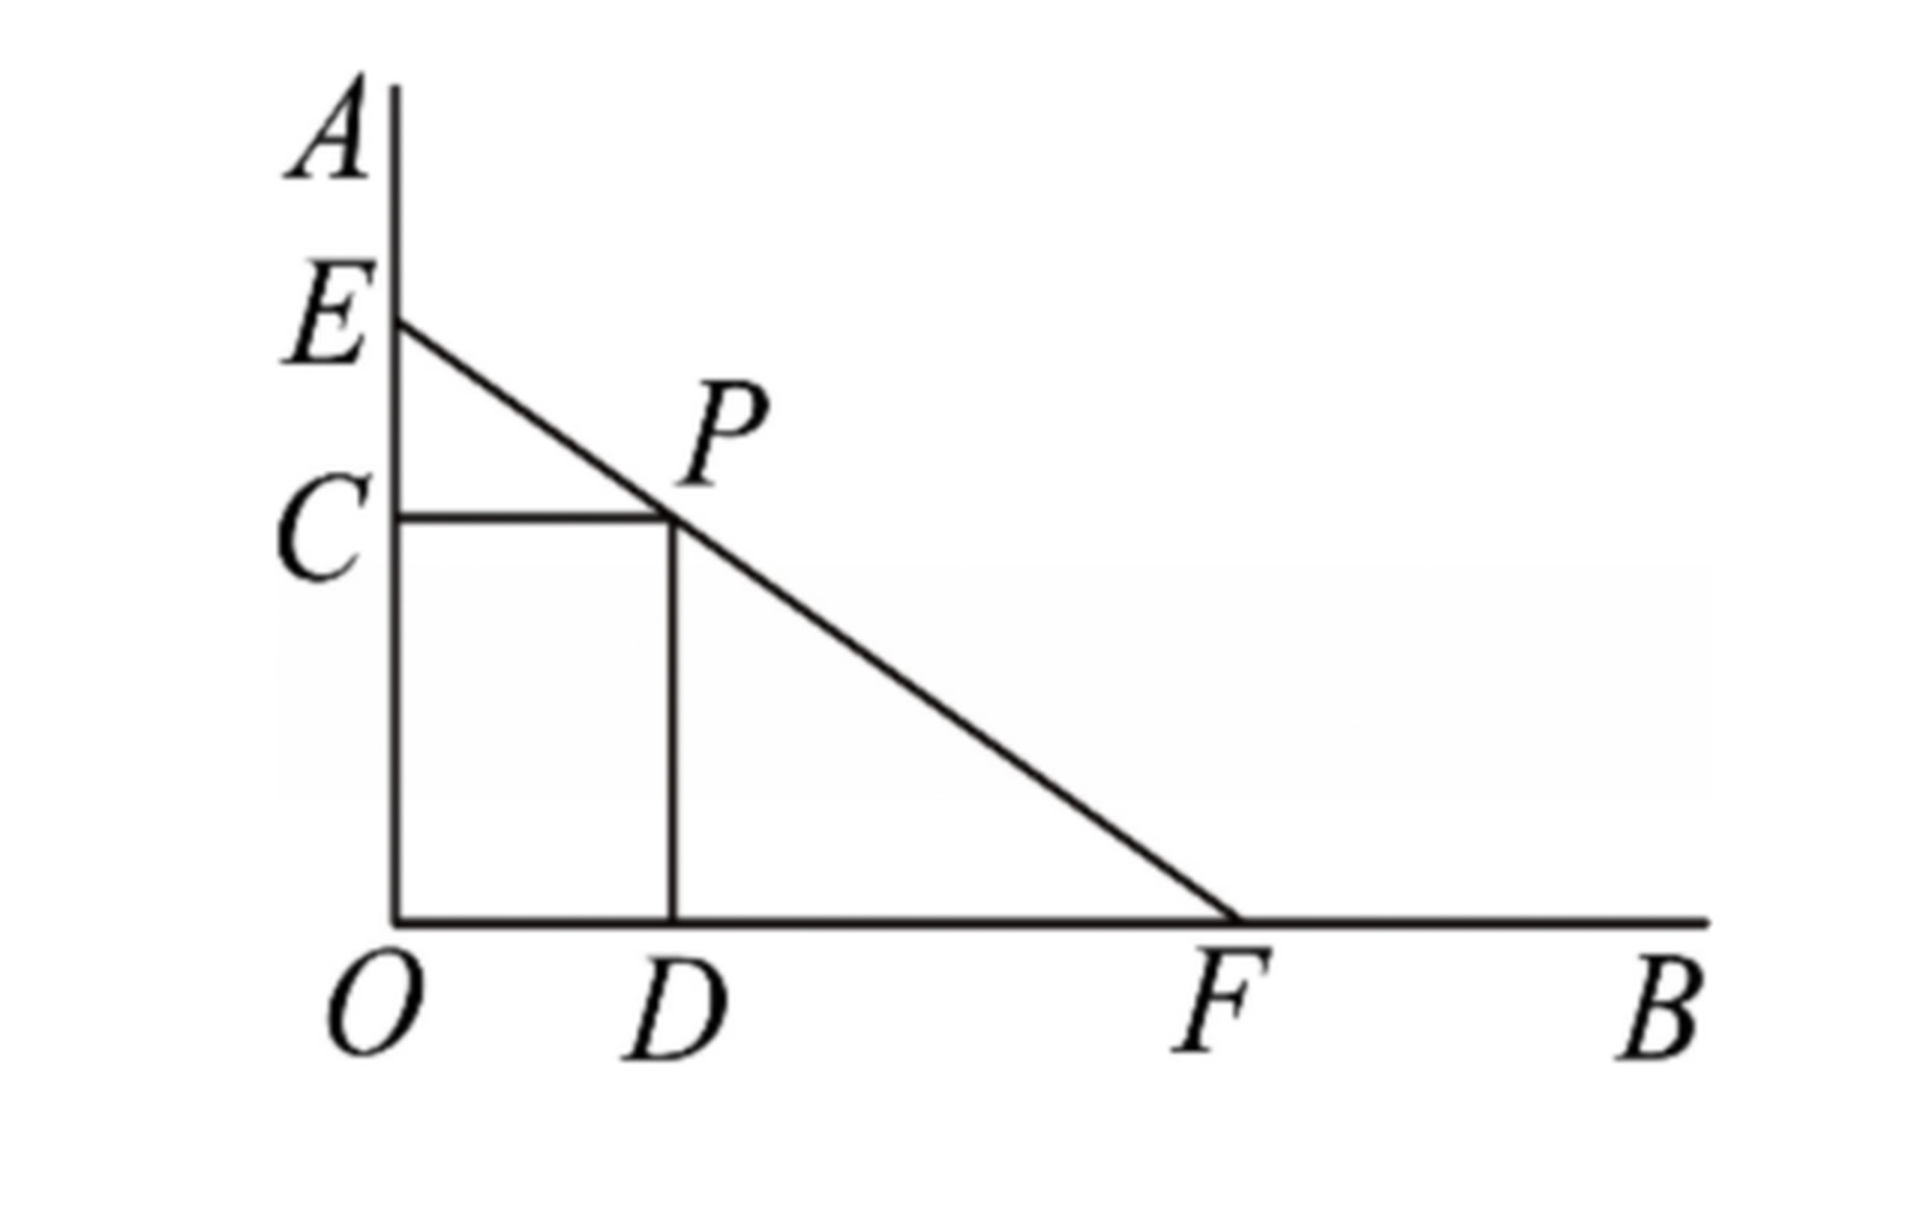
\includegraphics[width=0.32\textwidth]{figures/gao132_q18.png}
\end{center}

\ifanswer
\solbegin
\step{(1) 由题意得 $x\leq60$，}
\step{$\triangle PCE\sim\triangle FDP$，所以 $\dfrac{EC}{CP}=\dfrac{PD}{DF}$，即 $\dfrac{x}{25}=\dfrac{40}{DF}$，得 $DF=\dfrac{1000}{x}$m，}
\step{所以 $OF=OD+DF=\left(25+\dfrac{1000}x\right)$m，}
\step{所以 $25+\dfrac{1000}x\leq100$，解得 $x\geq\dfrac{40}3$；}
\step{综上，$\dfrac{40}3\leq x\leq60$；}
\step{(2) 由 $OE=OC+CE=(40+x)$m，}
\step{所以 $S=\dfrac12 OF\cdot OE=\dfrac12\left(25+\dfrac{1000}x\right)(40+x)$}
\step{$=\dfrac12\left(1000+25x+\dfrac{40000}x+1000\right)$m$^2$，}
\step{由基本不等式得 $S\geq\dfrac12\left(2000+2\sqrt{25x\cdot\dfrac{40000}x}\right)=2000$m$^2$，}
\step{当且仅当 $25x=\dfrac{40000}x$，即 $x=40$ 时取等号，}
\step{故 $EC=40$m 时，$S$ 取得最小值，为 $2000$m$^2$.}
\solend
\fi

\item 已知 $a>0$，$b>0$，请选择适当的方法证明.

(1) 若 $a\ne b$，证明：$a^3+b^3>a^2b+ab^2$；

(2) 若 $ab=1$，证明：$a^2+a<2$ 与 $b^2+b<2$ 不能同时成立.

\ifanswer
\solbegin
\step{(1) 因为 $a>0$，$b>0$，$a\ne b$，}
\step{所以 $a^3+b^3-a^2b-ab^2=a^2(a-b)+b^2(b-a)$}
\step{$=(a^2-b^2)(a-b)=(a-b)^2(a+b)>0$，所以 $a^3+b^3>a^2b+ab^2$.}
\step{(2) 假设 $a^2+a<2$ 与 $b^2+b<2$ 同时成立，所以 $-2<a<1,-2<b<1$，}
\step{又因为 $a>0,b>0$，所以 $0<a<1,0<b<1$，}
\step{所以 $0<ab<1$，这与 $ab=1$ 矛盾，}
\step{故 $a^2+a<2$ 与 $b^2+b<2$ 不可能同时成立.}
\solend
\fi

\item 若设 $M(a,n)=\lvert ax-1\rvert+\lvert ax-2\rvert+\cdots+\lvert ax-n\rvert$ 为曼哈顿扩张距离，它由 $n$ 个绝对值之和组成，其中 $n$ 为正整数.

(1) 若 $M(2,1)\leq5$，求 $x$ 的取值范围；

(2) 若 $k\leq M(2,2)$ 对一切实数 $x$ 恒成立，求实数 $k$ 的取值范围；

(3) $M(2,6)$ 是否存在最小值？若存在，求出该最小值与此时实数 $x$ 的取值范围；若不存在，说明理由.

\ifanswer
\solbegin
\step{(1) $M(2,1)=\lvert2x-1\rvert\leq5$，则不等式可化为 $-5\leq2x-1\leq5$，解得 $-2\leq x\leq3$，}
\step{所以 $x$ 的取值范围为 $[-2,3]$.}
\step{(2) 因为 $k\leq M(2,2)=\lvert2x-1\rvert+\lvert2x-2\rvert$ 对一切实数 $x$ 恒成立，}
\step{又 $\lvert2x-1\rvert+\lvert2x-2\rvert\geq\lvert(2x-1)-(2x-2)\rvert=1$，}
\step{当且仅当 $(2x-1)(2x-2)\leq0$，即 $\dfrac12\leq x\leq1$ 时取等号，}
\step{故 $k\leq1$，所以实数 $k$ 的取值范围为 $(-\infty,1]$.}
\step{(3) $M(2,6)=\lvert2x-1\rvert+\lvert2x-2\rvert+\lvert2x-3\rvert+\lvert2x-4\rvert+\lvert2x-5\rvert+\lvert2x-6\rvert$}
\step{$=2\left(\left\lvert x-\dfrac12\right\rvert+\lvert x-1\rvert+\left\lvert x-\dfrac32\right\rvert+\lvert x-2\rvert+\left\lvert x-\dfrac52\right\rvert+\lvert x-3\rvert\right)$，}
\step{其中 $\left\lvert x-\dfrac12\right\rvert+\lvert x-1\rvert+\left\lvert x-\dfrac32\right\rvert+\lvert x-2\rvert+\left\lvert x-\dfrac52\right\rvert+\lvert x-3\rvert$ 的几何意义为}
\step{在数轴上一点 $x$ 到 $\dfrac12,1,\dfrac32,2,\dfrac52,3$ 的距离之和，}
\step{要想距离之和最小，其中 $x\in\left[\dfrac12,3\right]$ 时，$\left\lvert x-\dfrac12\right\rvert+\lvert x-3\rvert$ 取得最小值，}
\step{当 $x\in\left[1,\dfrac52\right]$ 时，$\lvert x-1\rvert+\left\lvert x-\dfrac52\right\rvert$ 取得最小值，}
\step{当 $x\in\left[\dfrac32,2\right]$ 时，$\left\lvert x-\dfrac32\right\rvert+\lvert x-2\rvert$ 取得最小值，}
\step{综上，当 $x\in\left[\dfrac32,2\right]$ 时，$\left\lvert x-\dfrac12\right\rvert+\lvert x-1\rvert+\left\lvert x-\dfrac32\right\rvert+\lvert x-2\rvert+\left\lvert x-\dfrac52\right\rvert+\lvert x-3\rvert$}
\step{取得最小值，最小值为 $3-\dfrac12+\dfrac52-1+2-\dfrac32=\dfrac92$，}
\step{故 $M(2,6)=2\left(\left\lvert x-\dfrac12\right\rvert+\lvert x-1\rvert+\left\lvert x-\dfrac32\right\rvert+\lvert x-2\rvert+\left\lvert x-\dfrac52\right\rvert+\lvert x-3\rvert\right)$ 的}
\step{最小值为 $9$.}
\solend
\fi

\item 已知集合 $A=\{a_1,a_2,\cdots,a_n\}(0\leq a_1<a_2<\cdots<a_n,n\in\N,n\geq3)$ 具有性质 $Q$：对任意 $i,j(1\leq i\leq j\leq n)$，$a_i+a_j$ 与 $a_j-a_i$ 至少有一个属于集合 $A$；

(1) 判断集合 $M=\{0,2,4\}$ 与 $N=\{2,3,4\}$ 是否具有性质 $Q$，并说明理由；

(2) 已知 $A=\{a_1,a_2,a_3\}$ 具有性质 $Q$，当 $a_2=2026$ 时，求集合 $A$；

(3) 已知 $B=\{b_1,b_2,\cdots,b_{2026}\}$ 具有性质 $Q$，求 $\dfrac{b_1+b_2+\cdots+b_{2026}}{b_{2026}}$ 的值；

\ifanswer
\solbegin
\step{(1) 集合 $M=\{0,2,4\}$ 中，}
\step{因为 $0+2\in M,0+4\in M,4-2\in M,0\pm0=0\in M$，}
\step{$2+2=4\in M,2-2=0\in M,4-4=0\in M$，所以集合 $M$ 具有性质 $Q$；}
\step{集合 $N=\{2,3,4\}$ 中，因为 $3+3=6\notin N,3-3=0\notin N$，}
\step{所以集合 $N$ 不具有性质 $Q$.}
\step{(2) 因为 $a_1<a_2<a_3$，且 $A=\{a_1,a_2,a_3\}$ 具有性质 $Q$，}
\step{所以 $a_3+a_3\notin A,a_3-a_3=0\in A$，则 $a_1=0$，}
\step{又因为 $a_2+a_3>a_3$，所以 $a_2+a_3\notin A$，则 $a_3-a_2\in A$，}
\step{由集合的互异性得 $a_3-a_2=a_2$，而 $a_2=2026$，所以 $a_3=4052$，}
\step{故 $A=\{0,2026,4052\}$；}
\step{(3) 先证明一般结论：$A=\{a_1,a_2,\cdots,a_n\}(0\leq a_1<a_2<\cdots<a_n,n\in\N,n\geq3)$}
\step{具有性质 $Q$，则 $a_1+a_2+a_3+\cdots+a_n=\dfrac n2 a_n$.}
\step{因为 $A=\{a_1,a_2,\cdots,a_n\}(0\leq a_1<a_2<\cdots<a_n,n\in\N,n\geq3)$ 具有性质 $Q$，}
\step{所以 $a_n+a_n\notin A$，则 $a_n-a_n=0\in A$，则 $a_1=0$.}
\step{又因为 $0\leq a_1<a_2<\cdots<a_n$，所以 $0\leq a_n-a_n<a_n-a_{n-1}<\cdots<a_n-a_1$，}
\step{又因为 $a_n+a_{n-i}>a_n(i=1,2,\cdots,n-1)$，所以 $a_n+a_{n-i}\notin A$，}
\step{则 $a_n-a_{n-i}\in A$，}
\step{所以 $a_1=a_n-a_n,a_2=a_n-a_{n-1},a_3=a_n-a_{n-2},\cdots,a_n=a_n-a_1$.}
\step{所以 $a_1+a_2+a_3+\cdots+a_n$}
\step{$=(a_n-a_n)+(a_n-a_{n-1})+(a_n-a_{n-2})+\cdots+(a_n-a_1)$，}
\step{即 $a_1+a_2+a_3+\cdots+a_n=\dfrac n2 a_n$，}
\step{所以 $B=\{b_1,b_2,\cdots,b_{2026}\}$ 具有性质 $Q$，则 $b_1+b_2+\cdots+b_{2026}=\dfrac{2026}{2}b_{2026}$，}
\step{所以 $\dfrac{b_1+b_2+\cdots+b_{2026}}{b_{2026}}=\dfrac{2026}{2}=1013$.}
\solend
\fi

\end{enumerate}

% 行数复核：逐题数 \step 条数，合计 144 条（Q3：4；Q4：1；Q5：4；Q6：2；Q7：9；Q8：2；
% Q9：3；Q10：6；Q11：9；Q12：9；Q13：0；Q14：9；Q15：4；Q16：19；Q17：5；Q18：11；
% Q19：7；Q20：17；Q21：23），与原卷印刷行逐题相等（cases 块作一个印刷行计）。
% 第 13 题只印括号内答案、提 \ans{}，不计入 \step 账；第 14—16 题答案在解析末句，
% 括号内留空、不另提 \ans{}。

\end{document}
"
% 紧凑版：xelatex "\def\iscompact{1}% 高一132_川沙中学_期中.tex
%   —— 高一上数学"2026-2027 年川沙中学高一上期中"（试卷版/答案版）
% 试卷版：xelatex 高一132_川沙中学_期中.tex
% 答案版：xelatex "\def\isanswer{1}% 高一132_川沙中学_期中.tex
%   —— 高一上数学"2026-2027 年川沙中学高一上期中"（试卷版/答案版）
% 试卷版：xelatex 高一132_川沙中学_期中.tex
% 答案版：xelatex "\def\isanswer{1}% 高一132_川沙中学_期中.tex
%   —— 高一上数学"2026-2027 年川沙中学高一上期中"（试卷版/答案版）
% 试卷版：xelatex 高一132_川沙中学_期中.tex
% 答案版：xelatex "\def\isanswer{1}\input{高一132_川沙中学_期中.tex}"
% 紧凑版：xelatex "\def\iscompact{1}\input{高一132_川沙中学_期中.tex}"
%
% 原始材料：微信公众号"魔都数学加油站"文章，作者破晓，2026-11-14 19:00 发布；
% 连载"27学年高一132"，原文标题"27学年高一132——2026-2027年上海市川沙中学高一上期中"；
% 原文链接：https://mp.weixin.qq.com/s/VBG01CrUNMIYWWHhSfz8JQ。
% 正文为 11 张 PNG 页（01、04、06、07、09、11 为 2560x3620，02、03、05、08、10 为 4762x6735），
% 题目下印有【解析】，为讲评版。题目、解析均据原图转录；
% 卷面粉红色水印"魔都数学加油站"及公众号页脚未录入。全卷 2 幅插图：第 14 题四幅坐标图选项、
% 第 18 题矩形 OCPD 与小路 EF 示意图，均取原卷 04／07 页截图去水印。
%
% 卷首标题：原卷印作"2026-2027 年川沙中学高一上期中"（公众号标题中的"上海市"
% 卷面标题行没有，本稿照卷面），年份区间按全稿惯例排 en dash；原卷未印副标题，
% 本卷为期中卷、跨集合与常用逻辑用语／不等式／函数三章，按题目内容标为
% "集合与常用逻辑用语、不等式、函数"（与 125／126／128／129／131 同期中卷口径相同）：
% 集合与逻辑见 Q5、Q6、Q17、Q21，不等式见 Q3、Q4、Q9、Q10、Q12、Q13、Q15、Q16、Q19，
% 函数（幂函数、指数／对数、基本不等式应用）见 Q7、Q8、Q11、Q14、Q18、Q20。
%
% 题号体例：本卷共 19 题——一、填空题 3—12（10 题）、二、选择题 13—16（4 题）、
% 三、解答题 17—21（5 题）。三节分别 \setcounter{enumi}{2}／{12}／{16}。
%
% 与原卷的排版差异：
%   ① 原文从第 3 题起，本稿保留原题号（见上"题号体例"）；
%   ② 原卷每题下直接印【解析】，本稿按全稿惯例置于答案版；第 13 题答案 D 印在题干
%      括号内、无独立答案段，按 高一37／52／53／55／63／64／128／131 成例括号留空、
%      另提 \ans{$D$}；第 14—16 题答案在解析末句"故选 …"，括号内留空、不另提 \ans{}；
%   ③ 原卷未印副标题，本稿按"知识模块"口径补出；
%   ④ 原卷填空横线按全稿惯例排为 \blankline[4.4em]；选择题括号排 \mbox{（\quad）}、
%      选项段前按惯例加 \keepwithprev；解答题不留作答区（原卷为讲评版，与 109—131 同）；
%   ⑤ 原卷数集排斜体 $R^+$／$R$／$Z$／$N$，按全稿惯例改 \R^+／\R／\Z／\N；
%      绝对值排 \lvert…\rvert，集合描述竖线排 \mid；不等号按全稿惯例排 \leqslant／\geqslant；
%      补集照原卷上划线排 \overline{B}；
%   ⑥ 子题标号 (1)(2)(3) 原卷用半角括号，照录；第 14 题四幅坐标图选项按原卷 2×2 排布
%      合并裁为一张 \includegraphics（未用 TikZ 重绘，以保证与原卷一致），题前加
%      \needvspace{9cm} 守卫；第 18 题图取 07 页截图，题前按惯例加 \needvspace{7cm} 守卫
%      （照 高一120／127／129／131 成例），两者守卫都放在 \item 之前；
%   ⑦ 原卷 Q7 解析跨 01—02 页、Q10 解析跨 02—03 页、Q12 解析跨 03—04 页、
%      Q14 解析跨 04—05 页、Q16 解析在 06 页、Q18 解析跨 07—08 页、
%      Q20 解析跨 08—09 页、Q21 解析跨 10—11 页，本稿按题合并连续排版；
%      末页第 11 页为 Q21 (3) 解析的续尾，按实际印刷行单列。
%
% 判别式字形：第 10 题 $\triangle=4(a-1)^2+16(a-1)<0$、第 11 题
%   $\triangle=4(m-2)^2-4(m^2-3m+3)=-4m+4>0$ 两处原卷均排 $\triangle$（等边、扁），
%   逐处放大核对、字形一致，照录 \triangle；与 高一129／131 同题排 $\Delta$（等腰、高）不同。
%   全卷 \triangle 兼作第 18 题「$\triangle PCE\sim\triangle FDP$」「$\triangle OEF$」的几何
%   三角形记号，全卷未出现 \Delta。
%
% 子集符号：第 5 题解析 $B\subseteq A$、第 17 题 (2) 解析 $A\subseteq B$ 均印带下划线，
%   照录 \subseteq；全卷未出现单线 \subset。
%
% 原卷存疑照录：
%   第 9 题题干作"充分非必要条件"、解析作"充分不必要条件"，措辞不同，照录；
%   第 10 题解析"当 $a-1=0$ 时，$-4\geq0$，不等式不成立，$a=1$ 满足题意"照录；
%   第 11 题解析"所以 $2(m-1)+\dfrac1{m-1}\leq-2\sqrt2$"由上一行 $2(1-m)+\dfrac1{1-m}\geq2\sqrt2$
%     直接变号得到，照录；
%   第 12 题解析"由 $x\in Z$，$-7<-2\sqrt{10}<-6$"与"即 $k^2+7k+10\leq0$，解得 $-5\leq k\leq-2$"照录；
%   第 16 题解析"令 $52\times(930+a)=-52$，解得 $a=-931$"（按式应为 $a=-931$ 之外的解）照录；
%   第 19 题 (2) 解析"所以 $-2<a<1,-2<b<1$"数学式内半角逗号，照录；
%   第 20 题 (3) 解析"最小值为 $3-\dfrac12+\dfrac52-1+2-\dfrac32=\dfrac92$"与
%     "故 $M(2,6)=\dots$ 的最小值为 9"两处结论并列，照录；
%   第 21 题 (1) 解析"$0+2\in M,0+4\in M,4-2\in M,0\pm0=0\in M$"、
%     "$2+2=4\in M,2-2=0\in M,4-4=0\in M$"、(3) 各连写等式内半角逗号，照录；
%   第 21 题 (3) 解析"即 $a_1+a_2+a_3+\cdots+a_n=\dfrac n2 a_n$，"句末用半角逗号，照录。
%
% 行数复核：见文末"行数复核"注（逐题 \step 条数与原卷印刷行逐题相等，cases 块作一个印刷行计）。
%   第 13 题只印括号内答案、提 \ans{}，不计入 \step 账；第 14—16 题答案在解析末句，
%   括号内留空、不另提 \ans{}。
%
\documentclass[a4paper,11pt]{article}
\usepackage{common}

\begin{document}

\examtitlest[3]{2026--2027 年川沙中学高一上期中}{集合与常用逻辑用语、不等式、函数}

\bigsec{一、填空题}

\begin{enumerate}
\setcounter{enumi}{2}

\item 已知 $a$、$b\in\R^+$ 且 $ab=2$，则 $a+2b$ 的最小值为\blankline[4.4em].

\ifanswer
\solbegin
\step{因为 $a\in\R^+$，$b\in\R^+$ 且 $ab=2$，}
\step{由基本不等式得 $a+2b\geq2\sqrt{a\cdot2b}=2\sqrt{2ab}=2\sqrt4=4$.}
\step{等号当且仅当 $a=2b$ 时成立，结合 $ab=2$ 解得 $b=1$，$a=2$，}
\step{所以 $a+2b$ 的最小值为 $4$.}
\solend
\fi

\item 如果幂函数 $f(x)=(m^2-3m-3)x^{m^2+m-3}$ 在 $(0,+\infty)$ 上是增函数，则实数 $m=$\blankline[4.4em].

\ifanswer
\solbegin
\step{由已知得 $\begin{cases}m^2-3m-3=1\\m^2+m-3>0\end{cases}$，所以 $m=4$.}
\solend
\fi

\item 已知集合 $A=\{1,2\}$，集合 $B=\{x\mid ax=6\}$，若 $A\cup B=A$，则 $a$ 的所有取值构成的集合为\blankline[4.4em].

\ifanswer
\solbegin
\step{因为 $A\cup B=A$，所以 $B\subseteq A$，}
\step{当 $a=0$ 时，$B=\varnothing$，满足 $B\subseteq A$；}
\step{当 $a\ne0$ 时，$B=\left\{\dfrac6a\right\}$，则 $\dfrac6a=1$ 或 $\dfrac6a=2$，解得 $a=6$ 或 $a=3$，}
\step{综上所述，$a$ 的所有取值构成的集合为 $\{0,3,6\}$.}
\solend
\fi

\item 设全集为 $\R$，$A=\{y\mid y=-x^2+2x+1\}$，$B=\{x\mid y=\ln(x-1)\}$，则 $A\cap B=$\blankline[4.4em].

\ifanswer
\solbegin
\step{$A=\{y\mid y=-x^2+2x+1\}=\{y\mid y=-(x-1)^2+2\}=\{y\mid y\leq2\}$，}
\step{$B=\{x\mid y=\ln(x-1)\}=\{x\mid x>1\}$，则 $A\cap B=(1,2]$.}
\solend
\fi

\item 已知 $x\in\R$，则方程 $\lvert 6-x\rvert+\lvert 6x-3\rvert=\lvert 5x+3\rvert$ 的解集为\blankline[4.4em].

\ifanswer
\solbegin
\step{当 $x<-\dfrac35$ 时，$6-x>0$，$6x-3<0$，$5x+3<0$，}
\step{原方程为 $6-x-6x+3=-5x-3$，解得 $x=6$，不满足 $x<-\dfrac35$；}
\step{当 $-\dfrac35\leq x\leq\dfrac12$ 时，$5x+3\geq0$，$6x-3<0$，$6-x>0$，}
\step{原方程为 $6-x+3-6x=5x+3$，解得 $x=\dfrac12$；}
\step{当 $\dfrac12<x\leq6$ 时，$5x+3>0$，$6x-3>0$，$6-x\geq0$，}
\step{原方程为 $6-x+6x-3=5x+3$，即 $0=0$，恒成立，所以 $\dfrac12<x\leq6$；}
\step{当 $x>6$ 时，$5x+3\geq0$，$6x-3>0$，$6-x<0$，}
\step{原方程为 $x-6+6x-3=5x+3$，解得 $x=6$，不满足 $x>6$；}
\step{综上 $\dfrac12\leq x\leq6$，所以原方程的解集为 $\left\{x\mid\dfrac12\leq x\leq6\right\}$.}
\solend
\fi

\item 已知 $\log_2 3=a,2^b=7$，用 $a,b$ 表示 $\log_{42}56$ 为\blankline[4.4em].

\ifanswer
\solbegin
\step{$\log_{42}56=\dfrac{\log_2 56}{\log_2 42}=\dfrac{\log_2(7\times8)}{\log_2(6\times7)}=\dfrac{\log_2 7+\log_2 8}{\log_2 6+\log_2 7}$}
\step{$=\dfrac{\log_2 7+\log_2 2^3}{\log_2 2+\log_2 3+\log_2 7}=\dfrac{b+3}{1+a+b}$.}
\solend
\fi

\item 已知 $\dfrac13<x<\dfrac12$ 是不等式 $\lvert x-m\rvert<1$ 成立的充分非必要条件，则 $m$ 的取值范围是\blankline[4.4em].

\ifanswer
\solbegin
\step{因为 $\lvert x-m\rvert<1$，所以 $-1<x-m<1$，所以 $m-1<x<m+1$，}
\step{所以 $m-1<x<m+1$ 成立的充分不必要条件是 $\dfrac13<x<\dfrac12$，}
\step{所以 $\begin{cases}m-1\leq\dfrac13\\m+1\geq\dfrac12\end{cases}$，解得 $-\dfrac12\leq m\leq\dfrac43$，故 $m$ 的取值范围是 $\left[-\dfrac12,\dfrac43\right]$.}
\solend
\fi

\item 若关于 $x$ 的不等式 $(a-1)x^2+2(a-1)x-4\geq0$ 的解集为空集，则 $a$ 的取值范围是\blankline[4.4em].

\ifanswer
\solbegin
\step{关于 $x$ 的不等式 $(a-1)x^2+2(a-1)x-4\geq0$ 的解集为 $\varnothing$，}
\step{当 $a-1=0$ 时，$-4\geq0$，不等式不成立，$a=1$ 满足题意；}
\step{当 $a-1>0$ 时，$a>1$，不等式的解集不为空集，不满足题意；}
\step{当 $a-1<0$ 时，$a<1$，当 $\triangle=4(a-1)^2+16(a-1)<0$ 时，即 $(a-1)(a+3)<0$，}
\step{解得 $-3<a<1$，满足题意；}
\step{综上，实数 $a$ 的取值范围是 $\{a\mid-3<a\leq1\}$.}
\solend
\fi

\item 已知关于 $x$ 的方程 $x^2+2(m-2)x+m^2-3m+3=0$ 有两个不相等的实数根 $x_1$、$x_2$，则 $\dfrac{mx_1}{x_1-1}+\dfrac{mx_2}{x_2-1}-\dfrac{2}{x_1+x_2-2}$ 的最大值为\blankline[4.4em].

\ifanswer
\solbegin
\step{关于 $x$ 的方程 $x^2+2(m-2)x+m^2-3m+3=0$ 有两个不相等的实数根 $x_1$、$x_2$，}
\step{则 $\triangle=4(m-2)^2-4(m^2-3m+3)=-4m+4>0$，得 $m<1$，}
\step{且 $x_1+x_2=-2(m-2)$，$x_1x_2=m^2-3m+3$，}
\step{$\dfrac{mx_1}{x_1-1}+\dfrac{mx_2}{x_2-1}-\dfrac{2}{x_1+x_2-2}=\dfrac{m[2x_1x_2-(x_1+x_2)]}{x_1x_2-(x_1+x_2)+1}+\dfrac1{m-1}$}
\step{$=\dfrac{2m(m-1)^2}{m^2-m}+\dfrac1{m-1}=2(m-1)+\dfrac1{m-1}$，}
\step{又因为 $m<1$，所以 $m-1<0$，则 $1-m>0$，}
\step{所以 $2(1-m)+\dfrac1{1-m}\geq2\sqrt{2(1-m)\cdot\dfrac1{1-m}}=2\sqrt2$，}
\step{当且仅当 $2(1-m)=\dfrac1{1-m}$ 时，即 $m=1-\dfrac{\sqrt2}2$ 时取等号，}
\step{所以 $2(m-1)+\dfrac1{m-1}\leq-2\sqrt2$，即 $\dfrac{mx_1}{x_1-1}+\dfrac{mx_2}{x_2-1}-\dfrac2{x_1+x_2-2}$ 的最大值为 $-2\sqrt2$.}
\solend
\fi

\item 若使集合 $A=\{x\mid(kx-k^2-10)(x-1)>0,x\in\Z\}$ 中的元素个数最少，则实数 $k$ 的取值范围是\blankline[4.4em].

\ifanswer
\solbegin
\step{由题意集合 $A=\{x\mid(kx-k^2-10)(x-1)>0,\ x\in\Z\}$，}
\step{$k=0$ 时，不等式解得 $x<1$，有无数个整数解；}
\step{$k\ne0$ 时，则不等式变形为 $k\left(x-k-\dfrac{10}k\right)(x-1)>0$，}
\step{当 $k>0$ 时，$k+\dfrac{10}k\geq2\sqrt{10}$，仅当 $k=\sqrt{10}$ 时等号成立，}
\step{此时不等式解得 $x>k+\dfrac{10}k$ 或 $x<1$，有无数个整数解；}
\step{当 $k<0$ 时，$k+\dfrac{10}k=-\left[(-k)+\left(-\dfrac{10}k\right)\right]\leq-2\sqrt{10}$，仅当 $k=-\sqrt{10}$ 时等号成立，}
\step{此时不等式解得 $k+\dfrac{10}k<x<1$，}
\step{由 $x\in\Z$，$-7<-2\sqrt{10}<-6$，要使集合 $A$ 中的元素最少，则 $k+\dfrac{10}k\geq-7$，}
\step{即 $k^2+7k+10\leq0$，解得 $-5\leq k\leq-2$，故实数 $k$ 的取值范围是 $[-5,-2]$.}
\solend
\fi

\end{enumerate}

\bigsec{二、选择题}

\begin{enumerate}
\setcounter{enumi}{12}

\item 下列说法正确的是\mbox{（\quad）}

\keepwithprev
A. 若 $a>b$，则 $\dfrac1a<\dfrac1b$\qquad\qquad B. 若 $a>b$，$c>d$，则 $ac>bd$

C. 若 $a>b$，则 $ac^2>bc^2$\qquad\qquad D. 若 $ac^2>bc^2$，则 $a>b$

\ifanswer
\ans{$D$}
\fi

% 第 14 题四幅坐标图选项是一整块，守卫放在 \item 之前
\needvspace{9cm}
\item 在同一坐标系内，函数 $y=x^a(a\ne0)$ 和 $y=ax-\dfrac1a$ 的图象可能是\mbox{（\quad）}

\keepwithprev
\begin{center}
% 四幅坐标图选项取原卷 04 页截图去粉色水印，按原卷 2×2 排布合并为一张
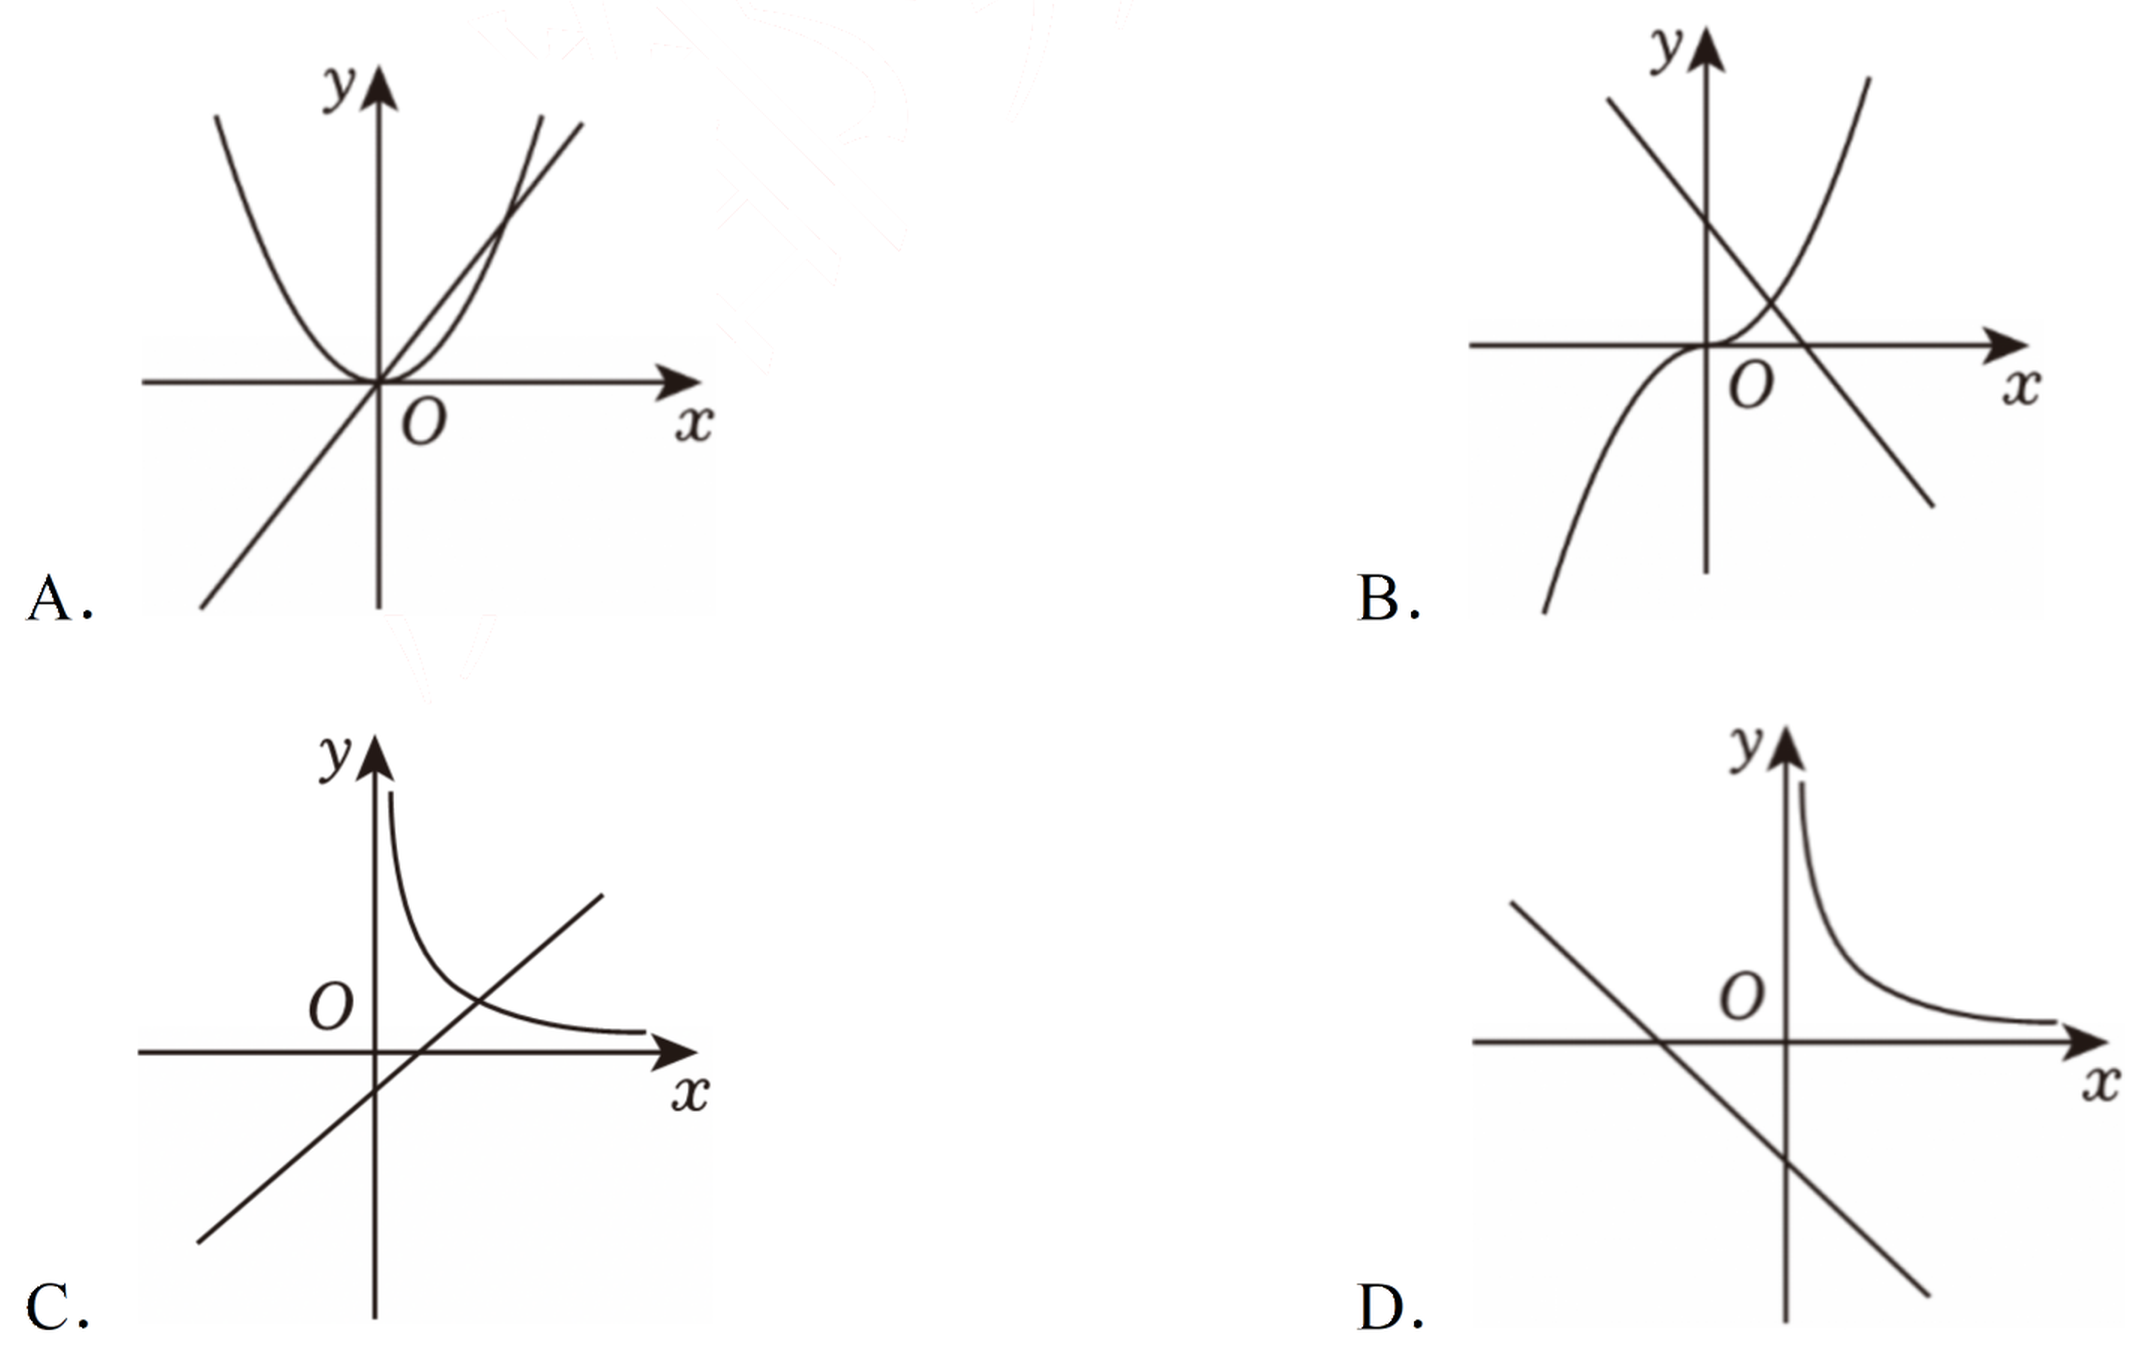
\includegraphics[width=0.80\textwidth]{figures/gao132_q14.png}
\end{center}

\ifanswer
\solbegin
\step{当 $a>0$ 时，$y=ax-\dfrac1a$ 严格增，当 $a<0$ 时，$y=ax-\dfrac1a$ 严格减，}
\step{对于 $A$，因为 $a\ne0$，所以直线 $y=ax-\dfrac1a$ 不过原点，故 $A$ 错误；}
\step{对于 $B$，由函数 $y=x^a(a\ne0)$ 的图象得 $a>1$，}
\step{由 $y=ax-\dfrac1a$ 的图象得 $a<0$，互相矛盾，故 $B$ 错误；}
\step{对于 $C$，由函数 $y=x^a(a\ne0)$ 的图象得 $a>1$，}
\step{由 $y=ax-\dfrac1a$ 的图象得 $a>0$ 且 $-\dfrac1a<0$，符合题意，故 $C$ 正确；}
\step{对于 $D$，由函数 $y=x^a(a\ne0)$ 的图象得 $a<0$，}
\step{由 $y=ax-\dfrac1a$ 的图象得 $a<0$ 且 $-\dfrac1a<0$，互相矛盾，故 $D$ 错误；}
\step{故选 $C$.}
\solend
\fi

\item 中国的 $5G$ 技术领先世界，在 $5G$ 技术中，最大数据传输速率 $C$ 取决于信道带宽 $W$，$C$ 与 $W$ 满足 $C=W\log_2\left(1+\dfrac SN\right)$，其中 $\dfrac SN$ 称为信噪比（单位：$dB$）. 若不改变带宽 $W$，初始信噪比 $\dfrac SN$ 为 $1000$，那么为了使 $C$ 增加 $30\%$，需要将信噪比 $\dfrac SN$ 从 $1000$ 提升至大约\mbox{（\quad）}

\keepwithprev
A. $5000$\qquad\qquad B. $6000$\qquad\qquad C. $7000$\qquad\qquad D. $8000$

\ifanswer
\solbegin
\step{由题意得 $\dfrac SN=1000$ 时，$C=W\log_2(1+1000)\approx W\log_2 1000$，}
\step{要使 $C$ 增加 $30\%$，则 $(1+30\%)C=W\log_2\left(1+\dfrac SN\right)$，即 $1.3C\approx W\log_2\dfrac SN$，}
\step{所以 $1.3\approx\log_{1000}\dfrac SN=\dfrac{\lg\frac SN}{\lg1000}$，所以 $\lg\dfrac SN=3.9$，所以 $\dfrac SN=10^{3.9}\approx8000$.}
\step{故选 $D$.}
\solend
\fi

\item 对于 $a\in\R$，设非空集合 $A=\left\{x\mid\dfrac{(x^2-930x+a)(x-52)}{x+a}=0\right\}$，记 $A$ 中的所有元素之和为 $S(a)$，所有元素之积为 $T(a)$，则下列说法中，不正确的是\mbox{（\quad）}

\keepwithprev
A. 存在实数 $a$，使得 $S(a)=930$

B. 存在实数 $a$，使得 $T(a)=517$

C. 不存在实数 $a$，使得 $T(a)=0$

D. 恰存在 $1$ 个实数 $a$，使得 $T(a)=-52$

\ifanswer
\solbegin
\step{由分式值为 $0$，得分子为 $0$ 且分母不为 $0$，}
\step{分子 $(x^2-930x+a)(x-52)=0$ 的根为 $x=52$}
\step{及方程 $x^2-930x+a=0$ 的两根 $x_1$，$x_2$，}
\step{由根与系数的关系得 $x_1+x_2=930$，$x_1\cdot x_2=a$，}
\step{分母限制 $x\ne-a$，需要剔除等于 $-a$ 的根，}
\step{选项 $A$，取 $a=-52$，$x=52$ 为增根舍去，集合 $A=\{x_1,x_2\}$，}
\step{元素之和 $S(a)=930$，故 $A$ 正确；}
\step{选项 $B$，当无增根时，$T(a)=52a$，令 $52a=517$，得 $a=\dfrac{517}{52}$，}
\step{验证无增根，存在这样的 $a$，故 $B$ 正确；}
\step{选项 $C$，若 $T(a)=0$，则 $0\in A$，代入分子得 $a=0$，}
\step{但 $a=0$ 时分母 $x\ne0$，$x=0$ 为增根，$0$ 不能属于集合 $A$，}
\step{故不存在 $a$ 使得 $T(a)=0$，故 $C$ 正确；}
\step{选项 $D$，当无增根时，令 $52a=-52$，得 $a=-1$；}
\step{当 $x=-a$ 是二次方程的根且不等于 $52$ 时，}
\step{令 $52\times(930+a)=-52$，解得 $a=-931$，验证符合条件；}
\step{当 $a=-52$ 时，$x=52$，舍去，}
\step{集合 $A=\{x_1,x_2\}$，$T(a)=a=-52$，得到两个满足条件的 $a$；}
\step{因此存在 $3$ 个满足条件的 $a$，故 $D$ 错误.}
\step{故选 $D$.}
\solend
\fi

\end{enumerate}

\bigsec{三、解答题}

\begin{enumerate}
\setcounter{enumi}{16}

\item 已知全集 $U=\R$，集合 $A=\left\{x\mid\dfrac{x}{x-3}<0\right\}$，$B=\{x\mid(x-a)(x+4-a)<0\}$.

(1) 当 $a=2$ 时，求 $\overline{B}$、$A\cap\overline{B}$；

(2) 若 $A\cap B=A$，求实数 $a$ 的取值范围.

\ifanswer
\solbegin
\step{(1) $\dfrac{x}{x-3}<0$，即 $x(x-3)<0$，解得 $A=\{x\mid0<x<3\}$，}
\step{当 $a=2$ 时，$B=\{x\mid(x-a)(x+4-a)<0\}=\{x\mid-2<x<2\}$，}
\step{则 $\overline{B}=\{x\mid x\leq-2$ 或 $x\geq2\}$，故 $A\cap\overline{B}=\{x\mid2\leq x<3\}$；}
\step{(2) $A\cap B=A$，则 $A\subseteq B$，故 $\begin{cases}a-4\leq0\\a\geq3\end{cases}$，解得 $3\leq a\leq4$，}
\step{故实数 $a$ 的取值范围是 $\{a\mid3\leq a\leq4\}$.}
\solend
\fi

% 第 18 题是"题干 + 图"约 7cm 的一整块，守卫放在 \item 之前
\needvspace{7cm}
\item 如图，$OA$、$OB$ 是两条长度足够长的互相垂直的笔直小路，矩形 $OCPD$ 的顶点 $C$、$D$ 分别在 $OA$、$OB$ 上，且该矩形区域内种满了荷花. 为了让观赏者有更好的观赏体验，现计划经过点 $P$ 修一条小路 $EF$，其中点 $E$ 在小路 $OA$ 上，点 $F$ 在小路 $OB$ 上，并在 $\triangle OEF$ 区域内种满荷花. 已知 $OD=25m$，$OC=40m$，且小路 $EF$ 要完全位于一个以 $O$ 为顶点的，边长为 $100$ m 的正方形内部（包括边界）. 记 $\triangle OEF$ 的面积为 $S$m$^2$.

(1) 设 $EC=x\cdot m$，试用 $x$ 表示 $OF$，并求 $x$ 的取值范围.

(2) 当 $EC$ 的长度为多少时，$S$ 取得最小值？最小值是多少？

\begin{center}
% 图取原卷 07 页截图去粉色水印，3× LANCZOS 放大
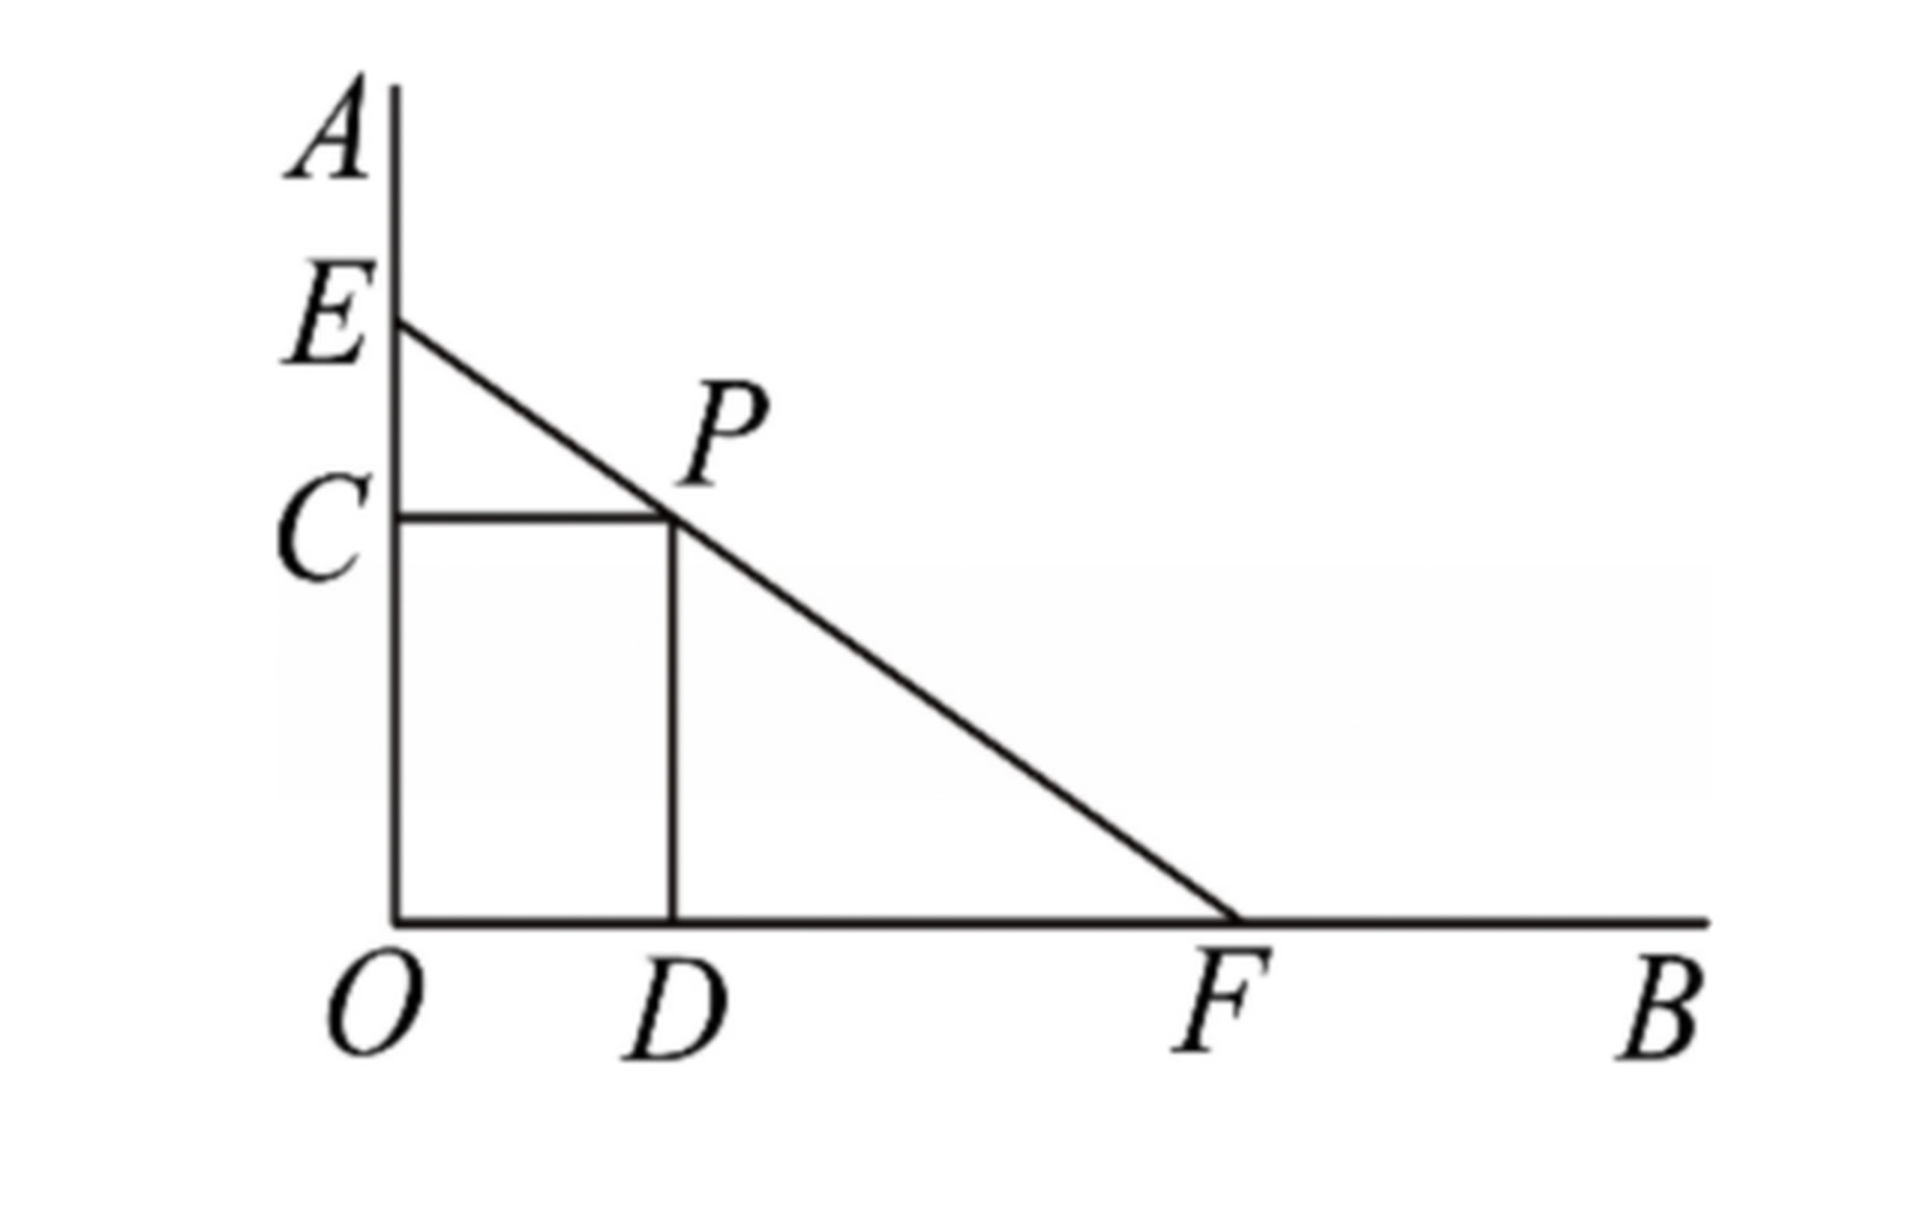
\includegraphics[width=0.32\textwidth]{figures/gao132_q18.png}
\end{center}

\ifanswer
\solbegin
\step{(1) 由题意得 $x\leq60$，}
\step{$\triangle PCE\sim\triangle FDP$，所以 $\dfrac{EC}{CP}=\dfrac{PD}{DF}$，即 $\dfrac{x}{25}=\dfrac{40}{DF}$，得 $DF=\dfrac{1000}{x}$m，}
\step{所以 $OF=OD+DF=\left(25+\dfrac{1000}x\right)$m，}
\step{所以 $25+\dfrac{1000}x\leq100$，解得 $x\geq\dfrac{40}3$；}
\step{综上，$\dfrac{40}3\leq x\leq60$；}
\step{(2) 由 $OE=OC+CE=(40+x)$m，}
\step{所以 $S=\dfrac12 OF\cdot OE=\dfrac12\left(25+\dfrac{1000}x\right)(40+x)$}
\step{$=\dfrac12\left(1000+25x+\dfrac{40000}x+1000\right)$m$^2$，}
\step{由基本不等式得 $S\geq\dfrac12\left(2000+2\sqrt{25x\cdot\dfrac{40000}x}\right)=2000$m$^2$，}
\step{当且仅当 $25x=\dfrac{40000}x$，即 $x=40$ 时取等号，}
\step{故 $EC=40$m 时，$S$ 取得最小值，为 $2000$m$^2$.}
\solend
\fi

\item 已知 $a>0$，$b>0$，请选择适当的方法证明.

(1) 若 $a\ne b$，证明：$a^3+b^3>a^2b+ab^2$；

(2) 若 $ab=1$，证明：$a^2+a<2$ 与 $b^2+b<2$ 不能同时成立.

\ifanswer
\solbegin
\step{(1) 因为 $a>0$，$b>0$，$a\ne b$，}
\step{所以 $a^3+b^3-a^2b-ab^2=a^2(a-b)+b^2(b-a)$}
\step{$=(a^2-b^2)(a-b)=(a-b)^2(a+b)>0$，所以 $a^3+b^3>a^2b+ab^2$.}
\step{(2) 假设 $a^2+a<2$ 与 $b^2+b<2$ 同时成立，所以 $-2<a<1,-2<b<1$，}
\step{又因为 $a>0,b>0$，所以 $0<a<1,0<b<1$，}
\step{所以 $0<ab<1$，这与 $ab=1$ 矛盾，}
\step{故 $a^2+a<2$ 与 $b^2+b<2$ 不可能同时成立.}
\solend
\fi

\item 若设 $M(a,n)=\lvert ax-1\rvert+\lvert ax-2\rvert+\cdots+\lvert ax-n\rvert$ 为曼哈顿扩张距离，它由 $n$ 个绝对值之和组成，其中 $n$ 为正整数.

(1) 若 $M(2,1)\leq5$，求 $x$ 的取值范围；

(2) 若 $k\leq M(2,2)$ 对一切实数 $x$ 恒成立，求实数 $k$ 的取值范围；

(3) $M(2,6)$ 是否存在最小值？若存在，求出该最小值与此时实数 $x$ 的取值范围；若不存在，说明理由.

\ifanswer
\solbegin
\step{(1) $M(2,1)=\lvert2x-1\rvert\leq5$，则不等式可化为 $-5\leq2x-1\leq5$，解得 $-2\leq x\leq3$，}
\step{所以 $x$ 的取值范围为 $[-2,3]$.}
\step{(2) 因为 $k\leq M(2,2)=\lvert2x-1\rvert+\lvert2x-2\rvert$ 对一切实数 $x$ 恒成立，}
\step{又 $\lvert2x-1\rvert+\lvert2x-2\rvert\geq\lvert(2x-1)-(2x-2)\rvert=1$，}
\step{当且仅当 $(2x-1)(2x-2)\leq0$，即 $\dfrac12\leq x\leq1$ 时取等号，}
\step{故 $k\leq1$，所以实数 $k$ 的取值范围为 $(-\infty,1]$.}
\step{(3) $M(2,6)=\lvert2x-1\rvert+\lvert2x-2\rvert+\lvert2x-3\rvert+\lvert2x-4\rvert+\lvert2x-5\rvert+\lvert2x-6\rvert$}
\step{$=2\left(\left\lvert x-\dfrac12\right\rvert+\lvert x-1\rvert+\left\lvert x-\dfrac32\right\rvert+\lvert x-2\rvert+\left\lvert x-\dfrac52\right\rvert+\lvert x-3\rvert\right)$，}
\step{其中 $\left\lvert x-\dfrac12\right\rvert+\lvert x-1\rvert+\left\lvert x-\dfrac32\right\rvert+\lvert x-2\rvert+\left\lvert x-\dfrac52\right\rvert+\lvert x-3\rvert$ 的几何意义为}
\step{在数轴上一点 $x$ 到 $\dfrac12,1,\dfrac32,2,\dfrac52,3$ 的距离之和，}
\step{要想距离之和最小，其中 $x\in\left[\dfrac12,3\right]$ 时，$\left\lvert x-\dfrac12\right\rvert+\lvert x-3\rvert$ 取得最小值，}
\step{当 $x\in\left[1,\dfrac52\right]$ 时，$\lvert x-1\rvert+\left\lvert x-\dfrac52\right\rvert$ 取得最小值，}
\step{当 $x\in\left[\dfrac32,2\right]$ 时，$\left\lvert x-\dfrac32\right\rvert+\lvert x-2\rvert$ 取得最小值，}
\step{综上，当 $x\in\left[\dfrac32,2\right]$ 时，$\left\lvert x-\dfrac12\right\rvert+\lvert x-1\rvert+\left\lvert x-\dfrac32\right\rvert+\lvert x-2\rvert+\left\lvert x-\dfrac52\right\rvert+\lvert x-3\rvert$}
\step{取得最小值，最小值为 $3-\dfrac12+\dfrac52-1+2-\dfrac32=\dfrac92$，}
\step{故 $M(2,6)=2\left(\left\lvert x-\dfrac12\right\rvert+\lvert x-1\rvert+\left\lvert x-\dfrac32\right\rvert+\lvert x-2\rvert+\left\lvert x-\dfrac52\right\rvert+\lvert x-3\rvert\right)$ 的}
\step{最小值为 $9$.}
\solend
\fi

\item 已知集合 $A=\{a_1,a_2,\cdots,a_n\}(0\leq a_1<a_2<\cdots<a_n,n\in\N,n\geq3)$ 具有性质 $Q$：对任意 $i,j(1\leq i\leq j\leq n)$，$a_i+a_j$ 与 $a_j-a_i$ 至少有一个属于集合 $A$；

(1) 判断集合 $M=\{0,2,4\}$ 与 $N=\{2,3,4\}$ 是否具有性质 $Q$，并说明理由；

(2) 已知 $A=\{a_1,a_2,a_3\}$ 具有性质 $Q$，当 $a_2=2026$ 时，求集合 $A$；

(3) 已知 $B=\{b_1,b_2,\cdots,b_{2026}\}$ 具有性质 $Q$，求 $\dfrac{b_1+b_2+\cdots+b_{2026}}{b_{2026}}$ 的值；

\ifanswer
\solbegin
\step{(1) 集合 $M=\{0,2,4\}$ 中，}
\step{因为 $0+2\in M,0+4\in M,4-2\in M,0\pm0=0\in M$，}
\step{$2+2=4\in M,2-2=0\in M,4-4=0\in M$，所以集合 $M$ 具有性质 $Q$；}
\step{集合 $N=\{2,3,4\}$ 中，因为 $3+3=6\notin N,3-3=0\notin N$，}
\step{所以集合 $N$ 不具有性质 $Q$.}
\step{(2) 因为 $a_1<a_2<a_3$，且 $A=\{a_1,a_2,a_3\}$ 具有性质 $Q$，}
\step{所以 $a_3+a_3\notin A,a_3-a_3=0\in A$，则 $a_1=0$，}
\step{又因为 $a_2+a_3>a_3$，所以 $a_2+a_3\notin A$，则 $a_3-a_2\in A$，}
\step{由集合的互异性得 $a_3-a_2=a_2$，而 $a_2=2026$，所以 $a_3=4052$，}
\step{故 $A=\{0,2026,4052\}$；}
\step{(3) 先证明一般结论：$A=\{a_1,a_2,\cdots,a_n\}(0\leq a_1<a_2<\cdots<a_n,n\in\N,n\geq3)$}
\step{具有性质 $Q$，则 $a_1+a_2+a_3+\cdots+a_n=\dfrac n2 a_n$.}
\step{因为 $A=\{a_1,a_2,\cdots,a_n\}(0\leq a_1<a_2<\cdots<a_n,n\in\N,n\geq3)$ 具有性质 $Q$，}
\step{所以 $a_n+a_n\notin A$，则 $a_n-a_n=0\in A$，则 $a_1=0$.}
\step{又因为 $0\leq a_1<a_2<\cdots<a_n$，所以 $0\leq a_n-a_n<a_n-a_{n-1}<\cdots<a_n-a_1$，}
\step{又因为 $a_n+a_{n-i}>a_n(i=1,2,\cdots,n-1)$，所以 $a_n+a_{n-i}\notin A$，}
\step{则 $a_n-a_{n-i}\in A$，}
\step{所以 $a_1=a_n-a_n,a_2=a_n-a_{n-1},a_3=a_n-a_{n-2},\cdots,a_n=a_n-a_1$.}
\step{所以 $a_1+a_2+a_3+\cdots+a_n$}
\step{$=(a_n-a_n)+(a_n-a_{n-1})+(a_n-a_{n-2})+\cdots+(a_n-a_1)$，}
\step{即 $a_1+a_2+a_3+\cdots+a_n=\dfrac n2 a_n$，}
\step{所以 $B=\{b_1,b_2,\cdots,b_{2026}\}$ 具有性质 $Q$，则 $b_1+b_2+\cdots+b_{2026}=\dfrac{2026}{2}b_{2026}$，}
\step{所以 $\dfrac{b_1+b_2+\cdots+b_{2026}}{b_{2026}}=\dfrac{2026}{2}=1013$.}
\solend
\fi

\end{enumerate}

% 行数复核：逐题数 \step 条数，合计 144 条（Q3：4；Q4：1；Q5：4；Q6：2；Q7：9；Q8：2；
% Q9：3；Q10：6；Q11：9；Q12：9；Q13：0；Q14：9；Q15：4；Q16：19；Q17：5；Q18：11；
% Q19：7；Q20：17；Q21：23），与原卷印刷行逐题相等（cases 块作一个印刷行计）。
% 第 13 题只印括号内答案、提 \ans{}，不计入 \step 账；第 14—16 题答案在解析末句，
% 括号内留空、不另提 \ans{}。

\end{document}
"
% 紧凑版：xelatex "\def\iscompact{1}% 高一132_川沙中学_期中.tex
%   —— 高一上数学"2026-2027 年川沙中学高一上期中"（试卷版/答案版）
% 试卷版：xelatex 高一132_川沙中学_期中.tex
% 答案版：xelatex "\def\isanswer{1}\input{高一132_川沙中学_期中.tex}"
% 紧凑版：xelatex "\def\iscompact{1}\input{高一132_川沙中学_期中.tex}"
%
% 原始材料：微信公众号"魔都数学加油站"文章，作者破晓，2026-11-14 19:00 发布；
% 连载"27学年高一132"，原文标题"27学年高一132——2026-2027年上海市川沙中学高一上期中"；
% 原文链接：https://mp.weixin.qq.com/s/VBG01CrUNMIYWWHhSfz8JQ。
% 正文为 11 张 PNG 页（01、04、06、07、09、11 为 2560x3620，02、03、05、08、10 为 4762x6735），
% 题目下印有【解析】，为讲评版。题目、解析均据原图转录；
% 卷面粉红色水印"魔都数学加油站"及公众号页脚未录入。全卷 2 幅插图：第 14 题四幅坐标图选项、
% 第 18 题矩形 OCPD 与小路 EF 示意图，均取原卷 04／07 页截图去水印。
%
% 卷首标题：原卷印作"2026-2027 年川沙中学高一上期中"（公众号标题中的"上海市"
% 卷面标题行没有，本稿照卷面），年份区间按全稿惯例排 en dash；原卷未印副标题，
% 本卷为期中卷、跨集合与常用逻辑用语／不等式／函数三章，按题目内容标为
% "集合与常用逻辑用语、不等式、函数"（与 125／126／128／129／131 同期中卷口径相同）：
% 集合与逻辑见 Q5、Q6、Q17、Q21，不等式见 Q3、Q4、Q9、Q10、Q12、Q13、Q15、Q16、Q19，
% 函数（幂函数、指数／对数、基本不等式应用）见 Q7、Q8、Q11、Q14、Q18、Q20。
%
% 题号体例：本卷共 19 题——一、填空题 3—12（10 题）、二、选择题 13—16（4 题）、
% 三、解答题 17—21（5 题）。三节分别 \setcounter{enumi}{2}／{12}／{16}。
%
% 与原卷的排版差异：
%   ① 原文从第 3 题起，本稿保留原题号（见上"题号体例"）；
%   ② 原卷每题下直接印【解析】，本稿按全稿惯例置于答案版；第 13 题答案 D 印在题干
%      括号内、无独立答案段，按 高一37／52／53／55／63／64／128／131 成例括号留空、
%      另提 \ans{$D$}；第 14—16 题答案在解析末句"故选 …"，括号内留空、不另提 \ans{}；
%   ③ 原卷未印副标题，本稿按"知识模块"口径补出；
%   ④ 原卷填空横线按全稿惯例排为 \blankline[4.4em]；选择题括号排 \mbox{（\quad）}、
%      选项段前按惯例加 \keepwithprev；解答题不留作答区（原卷为讲评版，与 109—131 同）；
%   ⑤ 原卷数集排斜体 $R^+$／$R$／$Z$／$N$，按全稿惯例改 \R^+／\R／\Z／\N；
%      绝对值排 \lvert…\rvert，集合描述竖线排 \mid；不等号按全稿惯例排 \leqslant／\geqslant；
%      补集照原卷上划线排 \overline{B}；
%   ⑥ 子题标号 (1)(2)(3) 原卷用半角括号，照录；第 14 题四幅坐标图选项按原卷 2×2 排布
%      合并裁为一张 \includegraphics（未用 TikZ 重绘，以保证与原卷一致），题前加
%      \needvspace{9cm} 守卫；第 18 题图取 07 页截图，题前按惯例加 \needvspace{7cm} 守卫
%      （照 高一120／127／129／131 成例），两者守卫都放在 \item 之前；
%   ⑦ 原卷 Q7 解析跨 01—02 页、Q10 解析跨 02—03 页、Q12 解析跨 03—04 页、
%      Q14 解析跨 04—05 页、Q16 解析在 06 页、Q18 解析跨 07—08 页、
%      Q20 解析跨 08—09 页、Q21 解析跨 10—11 页，本稿按题合并连续排版；
%      末页第 11 页为 Q21 (3) 解析的续尾，按实际印刷行单列。
%
% 判别式字形：第 10 题 $\triangle=4(a-1)^2+16(a-1)<0$、第 11 题
%   $\triangle=4(m-2)^2-4(m^2-3m+3)=-4m+4>0$ 两处原卷均排 $\triangle$（等边、扁），
%   逐处放大核对、字形一致，照录 \triangle；与 高一129／131 同题排 $\Delta$（等腰、高）不同。
%   全卷 \triangle 兼作第 18 题「$\triangle PCE\sim\triangle FDP$」「$\triangle OEF$」的几何
%   三角形记号，全卷未出现 \Delta。
%
% 子集符号：第 5 题解析 $B\subseteq A$、第 17 题 (2) 解析 $A\subseteq B$ 均印带下划线，
%   照录 \subseteq；全卷未出现单线 \subset。
%
% 原卷存疑照录：
%   第 9 题题干作"充分非必要条件"、解析作"充分不必要条件"，措辞不同，照录；
%   第 10 题解析"当 $a-1=0$ 时，$-4\geq0$，不等式不成立，$a=1$ 满足题意"照录；
%   第 11 题解析"所以 $2(m-1)+\dfrac1{m-1}\leq-2\sqrt2$"由上一行 $2(1-m)+\dfrac1{1-m}\geq2\sqrt2$
%     直接变号得到，照录；
%   第 12 题解析"由 $x\in Z$，$-7<-2\sqrt{10}<-6$"与"即 $k^2+7k+10\leq0$，解得 $-5\leq k\leq-2$"照录；
%   第 16 题解析"令 $52\times(930+a)=-52$，解得 $a=-931$"（按式应为 $a=-931$ 之外的解）照录；
%   第 19 题 (2) 解析"所以 $-2<a<1,-2<b<1$"数学式内半角逗号，照录；
%   第 20 题 (3) 解析"最小值为 $3-\dfrac12+\dfrac52-1+2-\dfrac32=\dfrac92$"与
%     "故 $M(2,6)=\dots$ 的最小值为 9"两处结论并列，照录；
%   第 21 题 (1) 解析"$0+2\in M,0+4\in M,4-2\in M,0\pm0=0\in M$"、
%     "$2+2=4\in M,2-2=0\in M,4-4=0\in M$"、(3) 各连写等式内半角逗号，照录；
%   第 21 题 (3) 解析"即 $a_1+a_2+a_3+\cdots+a_n=\dfrac n2 a_n$，"句末用半角逗号，照录。
%
% 行数复核：见文末"行数复核"注（逐题 \step 条数与原卷印刷行逐题相等，cases 块作一个印刷行计）。
%   第 13 题只印括号内答案、提 \ans{}，不计入 \step 账；第 14—16 题答案在解析末句，
%   括号内留空、不另提 \ans{}。
%
\documentclass[a4paper,11pt]{article}
\usepackage{common}

\begin{document}

\examtitlest[3]{2026--2027 年川沙中学高一上期中}{集合与常用逻辑用语、不等式、函数}

\bigsec{一、填空题}

\begin{enumerate}
\setcounter{enumi}{2}

\item 已知 $a$、$b\in\R^+$ 且 $ab=2$，则 $a+2b$ 的最小值为\blankline[4.4em].

\ifanswer
\solbegin
\step{因为 $a\in\R^+$，$b\in\R^+$ 且 $ab=2$，}
\step{由基本不等式得 $a+2b\geq2\sqrt{a\cdot2b}=2\sqrt{2ab}=2\sqrt4=4$.}
\step{等号当且仅当 $a=2b$ 时成立，结合 $ab=2$ 解得 $b=1$，$a=2$，}
\step{所以 $a+2b$ 的最小值为 $4$.}
\solend
\fi

\item 如果幂函数 $f(x)=(m^2-3m-3)x^{m^2+m-3}$ 在 $(0,+\infty)$ 上是增函数，则实数 $m=$\blankline[4.4em].

\ifanswer
\solbegin
\step{由已知得 $\begin{cases}m^2-3m-3=1\\m^2+m-3>0\end{cases}$，所以 $m=4$.}
\solend
\fi

\item 已知集合 $A=\{1,2\}$，集合 $B=\{x\mid ax=6\}$，若 $A\cup B=A$，则 $a$ 的所有取值构成的集合为\blankline[4.4em].

\ifanswer
\solbegin
\step{因为 $A\cup B=A$，所以 $B\subseteq A$，}
\step{当 $a=0$ 时，$B=\varnothing$，满足 $B\subseteq A$；}
\step{当 $a\ne0$ 时，$B=\left\{\dfrac6a\right\}$，则 $\dfrac6a=1$ 或 $\dfrac6a=2$，解得 $a=6$ 或 $a=3$，}
\step{综上所述，$a$ 的所有取值构成的集合为 $\{0,3,6\}$.}
\solend
\fi

\item 设全集为 $\R$，$A=\{y\mid y=-x^2+2x+1\}$，$B=\{x\mid y=\ln(x-1)\}$，则 $A\cap B=$\blankline[4.4em].

\ifanswer
\solbegin
\step{$A=\{y\mid y=-x^2+2x+1\}=\{y\mid y=-(x-1)^2+2\}=\{y\mid y\leq2\}$，}
\step{$B=\{x\mid y=\ln(x-1)\}=\{x\mid x>1\}$，则 $A\cap B=(1,2]$.}
\solend
\fi

\item 已知 $x\in\R$，则方程 $\lvert 6-x\rvert+\lvert 6x-3\rvert=\lvert 5x+3\rvert$ 的解集为\blankline[4.4em].

\ifanswer
\solbegin
\step{当 $x<-\dfrac35$ 时，$6-x>0$，$6x-3<0$，$5x+3<0$，}
\step{原方程为 $6-x-6x+3=-5x-3$，解得 $x=6$，不满足 $x<-\dfrac35$；}
\step{当 $-\dfrac35\leq x\leq\dfrac12$ 时，$5x+3\geq0$，$6x-3<0$，$6-x>0$，}
\step{原方程为 $6-x+3-6x=5x+3$，解得 $x=\dfrac12$；}
\step{当 $\dfrac12<x\leq6$ 时，$5x+3>0$，$6x-3>0$，$6-x\geq0$，}
\step{原方程为 $6-x+6x-3=5x+3$，即 $0=0$，恒成立，所以 $\dfrac12<x\leq6$；}
\step{当 $x>6$ 时，$5x+3\geq0$，$6x-3>0$，$6-x<0$，}
\step{原方程为 $x-6+6x-3=5x+3$，解得 $x=6$，不满足 $x>6$；}
\step{综上 $\dfrac12\leq x\leq6$，所以原方程的解集为 $\left\{x\mid\dfrac12\leq x\leq6\right\}$.}
\solend
\fi

\item 已知 $\log_2 3=a,2^b=7$，用 $a,b$ 表示 $\log_{42}56$ 为\blankline[4.4em].

\ifanswer
\solbegin
\step{$\log_{42}56=\dfrac{\log_2 56}{\log_2 42}=\dfrac{\log_2(7\times8)}{\log_2(6\times7)}=\dfrac{\log_2 7+\log_2 8}{\log_2 6+\log_2 7}$}
\step{$=\dfrac{\log_2 7+\log_2 2^3}{\log_2 2+\log_2 3+\log_2 7}=\dfrac{b+3}{1+a+b}$.}
\solend
\fi

\item 已知 $\dfrac13<x<\dfrac12$ 是不等式 $\lvert x-m\rvert<1$ 成立的充分非必要条件，则 $m$ 的取值范围是\blankline[4.4em].

\ifanswer
\solbegin
\step{因为 $\lvert x-m\rvert<1$，所以 $-1<x-m<1$，所以 $m-1<x<m+1$，}
\step{所以 $m-1<x<m+1$ 成立的充分不必要条件是 $\dfrac13<x<\dfrac12$，}
\step{所以 $\begin{cases}m-1\leq\dfrac13\\m+1\geq\dfrac12\end{cases}$，解得 $-\dfrac12\leq m\leq\dfrac43$，故 $m$ 的取值范围是 $\left[-\dfrac12,\dfrac43\right]$.}
\solend
\fi

\item 若关于 $x$ 的不等式 $(a-1)x^2+2(a-1)x-4\geq0$ 的解集为空集，则 $a$ 的取值范围是\blankline[4.4em].

\ifanswer
\solbegin
\step{关于 $x$ 的不等式 $(a-1)x^2+2(a-1)x-4\geq0$ 的解集为 $\varnothing$，}
\step{当 $a-1=0$ 时，$-4\geq0$，不等式不成立，$a=1$ 满足题意；}
\step{当 $a-1>0$ 时，$a>1$，不等式的解集不为空集，不满足题意；}
\step{当 $a-1<0$ 时，$a<1$，当 $\triangle=4(a-1)^2+16(a-1)<0$ 时，即 $(a-1)(a+3)<0$，}
\step{解得 $-3<a<1$，满足题意；}
\step{综上，实数 $a$ 的取值范围是 $\{a\mid-3<a\leq1\}$.}
\solend
\fi

\item 已知关于 $x$ 的方程 $x^2+2(m-2)x+m^2-3m+3=0$ 有两个不相等的实数根 $x_1$、$x_2$，则 $\dfrac{mx_1}{x_1-1}+\dfrac{mx_2}{x_2-1}-\dfrac{2}{x_1+x_2-2}$ 的最大值为\blankline[4.4em].

\ifanswer
\solbegin
\step{关于 $x$ 的方程 $x^2+2(m-2)x+m^2-3m+3=0$ 有两个不相等的实数根 $x_1$、$x_2$，}
\step{则 $\triangle=4(m-2)^2-4(m^2-3m+3)=-4m+4>0$，得 $m<1$，}
\step{且 $x_1+x_2=-2(m-2)$，$x_1x_2=m^2-3m+3$，}
\step{$\dfrac{mx_1}{x_1-1}+\dfrac{mx_2}{x_2-1}-\dfrac{2}{x_1+x_2-2}=\dfrac{m[2x_1x_2-(x_1+x_2)]}{x_1x_2-(x_1+x_2)+1}+\dfrac1{m-1}$}
\step{$=\dfrac{2m(m-1)^2}{m^2-m}+\dfrac1{m-1}=2(m-1)+\dfrac1{m-1}$，}
\step{又因为 $m<1$，所以 $m-1<0$，则 $1-m>0$，}
\step{所以 $2(1-m)+\dfrac1{1-m}\geq2\sqrt{2(1-m)\cdot\dfrac1{1-m}}=2\sqrt2$，}
\step{当且仅当 $2(1-m)=\dfrac1{1-m}$ 时，即 $m=1-\dfrac{\sqrt2}2$ 时取等号，}
\step{所以 $2(m-1)+\dfrac1{m-1}\leq-2\sqrt2$，即 $\dfrac{mx_1}{x_1-1}+\dfrac{mx_2}{x_2-1}-\dfrac2{x_1+x_2-2}$ 的最大值为 $-2\sqrt2$.}
\solend
\fi

\item 若使集合 $A=\{x\mid(kx-k^2-10)(x-1)>0,x\in\Z\}$ 中的元素个数最少，则实数 $k$ 的取值范围是\blankline[4.4em].

\ifanswer
\solbegin
\step{由题意集合 $A=\{x\mid(kx-k^2-10)(x-1)>0,\ x\in\Z\}$，}
\step{$k=0$ 时，不等式解得 $x<1$，有无数个整数解；}
\step{$k\ne0$ 时，则不等式变形为 $k\left(x-k-\dfrac{10}k\right)(x-1)>0$，}
\step{当 $k>0$ 时，$k+\dfrac{10}k\geq2\sqrt{10}$，仅当 $k=\sqrt{10}$ 时等号成立，}
\step{此时不等式解得 $x>k+\dfrac{10}k$ 或 $x<1$，有无数个整数解；}
\step{当 $k<0$ 时，$k+\dfrac{10}k=-\left[(-k)+\left(-\dfrac{10}k\right)\right]\leq-2\sqrt{10}$，仅当 $k=-\sqrt{10}$ 时等号成立，}
\step{此时不等式解得 $k+\dfrac{10}k<x<1$，}
\step{由 $x\in\Z$，$-7<-2\sqrt{10}<-6$，要使集合 $A$ 中的元素最少，则 $k+\dfrac{10}k\geq-7$，}
\step{即 $k^2+7k+10\leq0$，解得 $-5\leq k\leq-2$，故实数 $k$ 的取值范围是 $[-5,-2]$.}
\solend
\fi

\end{enumerate}

\bigsec{二、选择题}

\begin{enumerate}
\setcounter{enumi}{12}

\item 下列说法正确的是\mbox{（\quad）}

\keepwithprev
A. 若 $a>b$，则 $\dfrac1a<\dfrac1b$\qquad\qquad B. 若 $a>b$，$c>d$，则 $ac>bd$

C. 若 $a>b$，则 $ac^2>bc^2$\qquad\qquad D. 若 $ac^2>bc^2$，则 $a>b$

\ifanswer
\ans{$D$}
\fi

% 第 14 题四幅坐标图选项是一整块，守卫放在 \item 之前
\needvspace{9cm}
\item 在同一坐标系内，函数 $y=x^a(a\ne0)$ 和 $y=ax-\dfrac1a$ 的图象可能是\mbox{（\quad）}

\keepwithprev
\begin{center}
% 四幅坐标图选项取原卷 04 页截图去粉色水印，按原卷 2×2 排布合并为一张
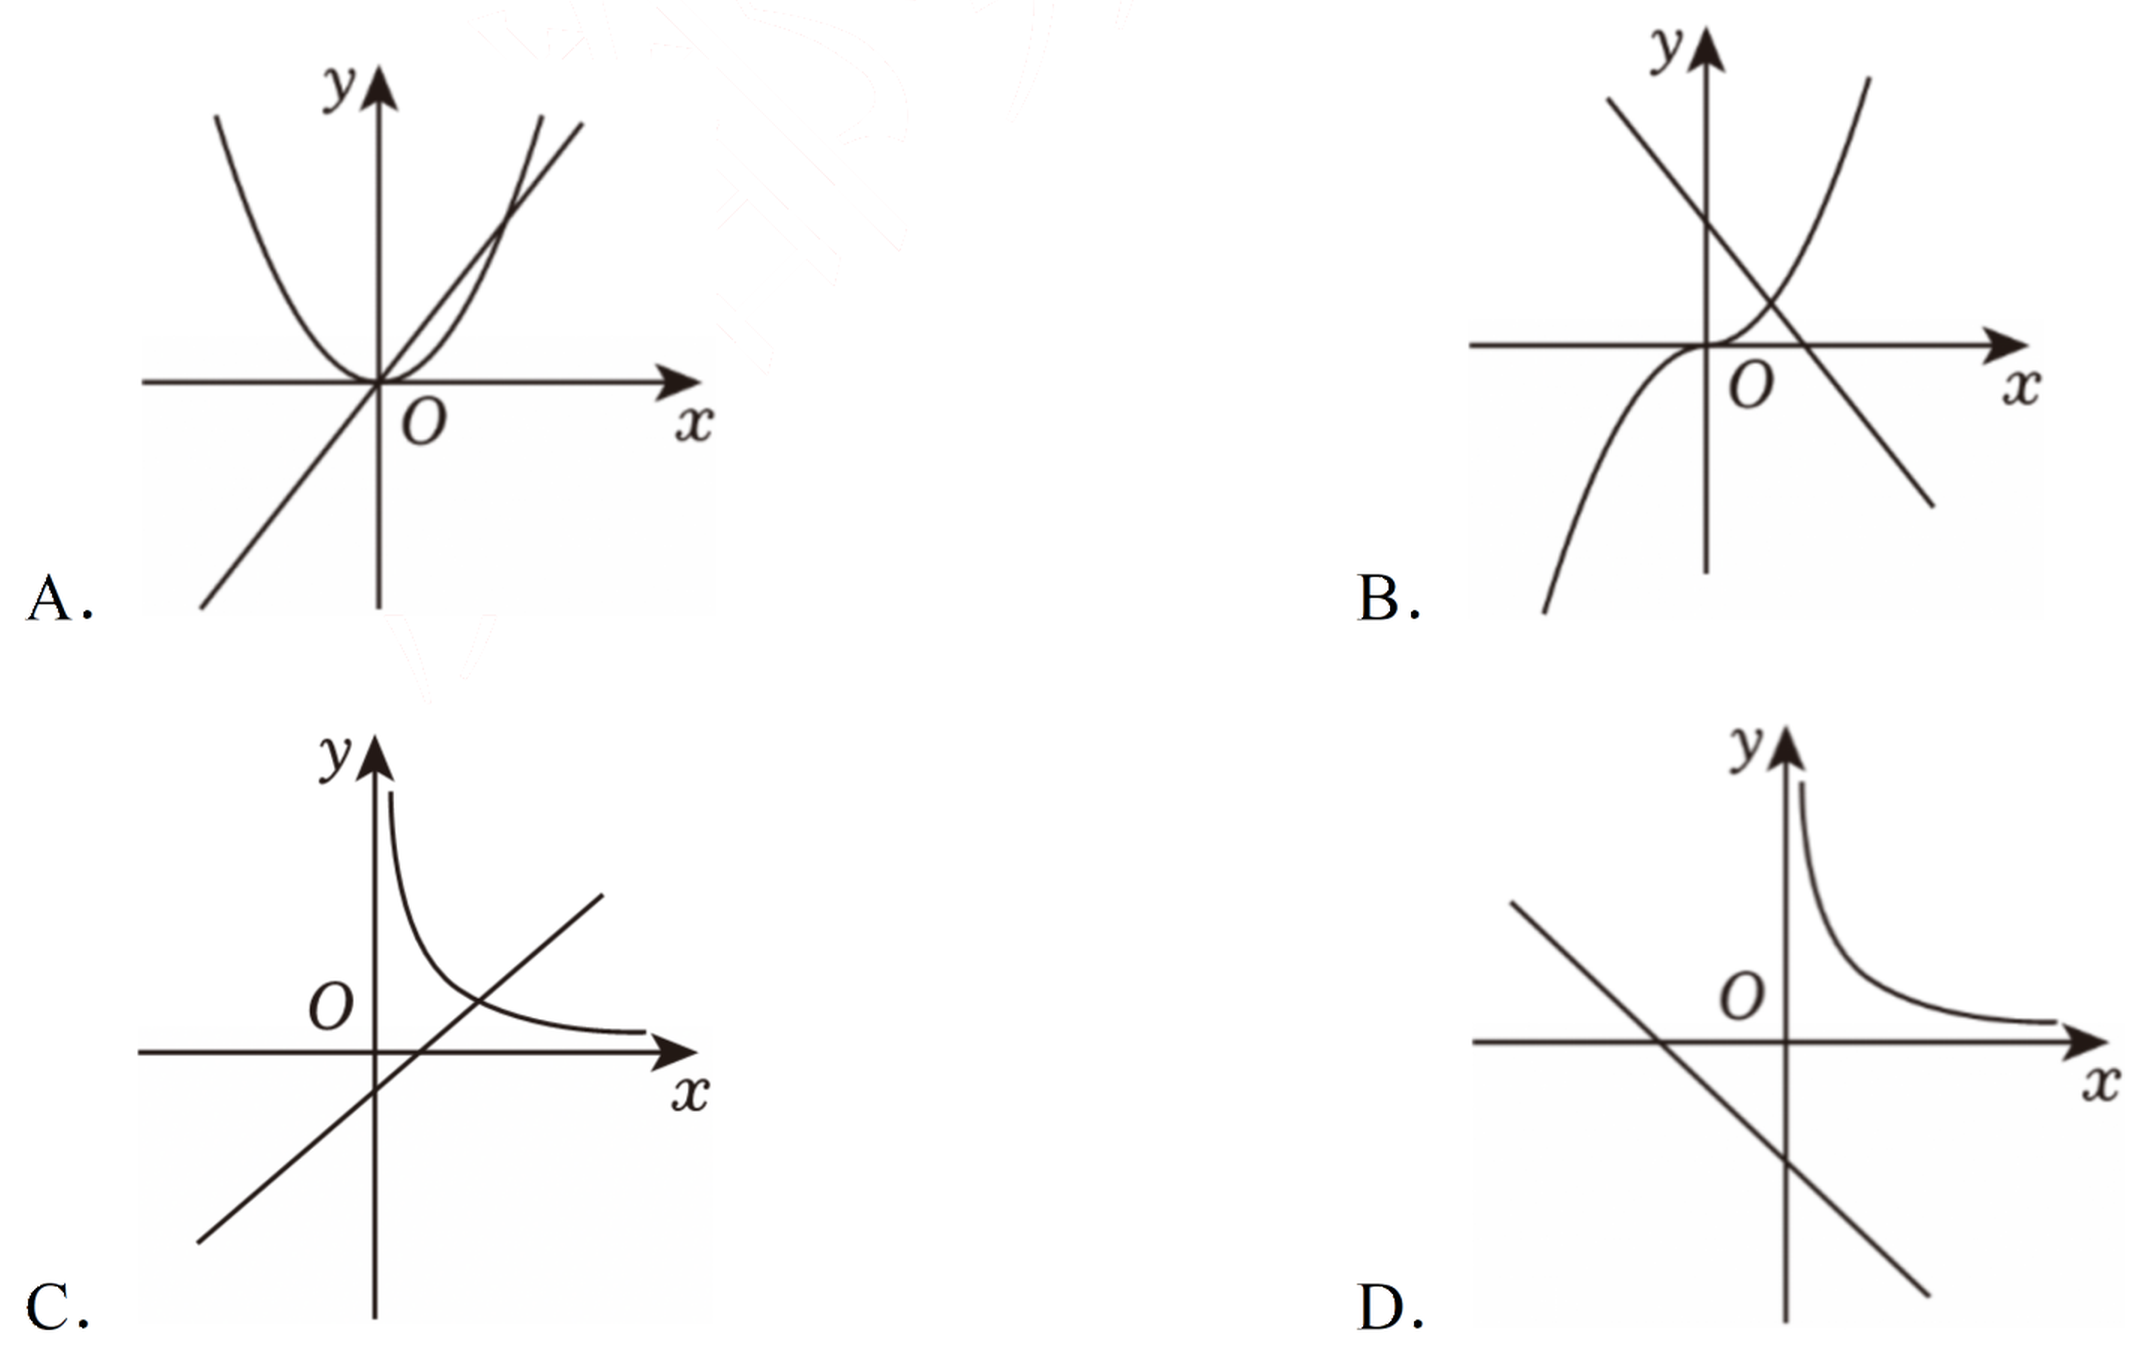
\includegraphics[width=0.80\textwidth]{figures/gao132_q14.png}
\end{center}

\ifanswer
\solbegin
\step{当 $a>0$ 时，$y=ax-\dfrac1a$ 严格增，当 $a<0$ 时，$y=ax-\dfrac1a$ 严格减，}
\step{对于 $A$，因为 $a\ne0$，所以直线 $y=ax-\dfrac1a$ 不过原点，故 $A$ 错误；}
\step{对于 $B$，由函数 $y=x^a(a\ne0)$ 的图象得 $a>1$，}
\step{由 $y=ax-\dfrac1a$ 的图象得 $a<0$，互相矛盾，故 $B$ 错误；}
\step{对于 $C$，由函数 $y=x^a(a\ne0)$ 的图象得 $a>1$，}
\step{由 $y=ax-\dfrac1a$ 的图象得 $a>0$ 且 $-\dfrac1a<0$，符合题意，故 $C$ 正确；}
\step{对于 $D$，由函数 $y=x^a(a\ne0)$ 的图象得 $a<0$，}
\step{由 $y=ax-\dfrac1a$ 的图象得 $a<0$ 且 $-\dfrac1a<0$，互相矛盾，故 $D$ 错误；}
\step{故选 $C$.}
\solend
\fi

\item 中国的 $5G$ 技术领先世界，在 $5G$ 技术中，最大数据传输速率 $C$ 取决于信道带宽 $W$，$C$ 与 $W$ 满足 $C=W\log_2\left(1+\dfrac SN\right)$，其中 $\dfrac SN$ 称为信噪比（单位：$dB$）. 若不改变带宽 $W$，初始信噪比 $\dfrac SN$ 为 $1000$，那么为了使 $C$ 增加 $30\%$，需要将信噪比 $\dfrac SN$ 从 $1000$ 提升至大约\mbox{（\quad）}

\keepwithprev
A. $5000$\qquad\qquad B. $6000$\qquad\qquad C. $7000$\qquad\qquad D. $8000$

\ifanswer
\solbegin
\step{由题意得 $\dfrac SN=1000$ 时，$C=W\log_2(1+1000)\approx W\log_2 1000$，}
\step{要使 $C$ 增加 $30\%$，则 $(1+30\%)C=W\log_2\left(1+\dfrac SN\right)$，即 $1.3C\approx W\log_2\dfrac SN$，}
\step{所以 $1.3\approx\log_{1000}\dfrac SN=\dfrac{\lg\frac SN}{\lg1000}$，所以 $\lg\dfrac SN=3.9$，所以 $\dfrac SN=10^{3.9}\approx8000$.}
\step{故选 $D$.}
\solend
\fi

\item 对于 $a\in\R$，设非空集合 $A=\left\{x\mid\dfrac{(x^2-930x+a)(x-52)}{x+a}=0\right\}$，记 $A$ 中的所有元素之和为 $S(a)$，所有元素之积为 $T(a)$，则下列说法中，不正确的是\mbox{（\quad）}

\keepwithprev
A. 存在实数 $a$，使得 $S(a)=930$

B. 存在实数 $a$，使得 $T(a)=517$

C. 不存在实数 $a$，使得 $T(a)=0$

D. 恰存在 $1$ 个实数 $a$，使得 $T(a)=-52$

\ifanswer
\solbegin
\step{由分式值为 $0$，得分子为 $0$ 且分母不为 $0$，}
\step{分子 $(x^2-930x+a)(x-52)=0$ 的根为 $x=52$}
\step{及方程 $x^2-930x+a=0$ 的两根 $x_1$，$x_2$，}
\step{由根与系数的关系得 $x_1+x_2=930$，$x_1\cdot x_2=a$，}
\step{分母限制 $x\ne-a$，需要剔除等于 $-a$ 的根，}
\step{选项 $A$，取 $a=-52$，$x=52$ 为增根舍去，集合 $A=\{x_1,x_2\}$，}
\step{元素之和 $S(a)=930$，故 $A$ 正确；}
\step{选项 $B$，当无增根时，$T(a)=52a$，令 $52a=517$，得 $a=\dfrac{517}{52}$，}
\step{验证无增根，存在这样的 $a$，故 $B$ 正确；}
\step{选项 $C$，若 $T(a)=0$，则 $0\in A$，代入分子得 $a=0$，}
\step{但 $a=0$ 时分母 $x\ne0$，$x=0$ 为增根，$0$ 不能属于集合 $A$，}
\step{故不存在 $a$ 使得 $T(a)=0$，故 $C$ 正确；}
\step{选项 $D$，当无增根时，令 $52a=-52$，得 $a=-1$；}
\step{当 $x=-a$ 是二次方程的根且不等于 $52$ 时，}
\step{令 $52\times(930+a)=-52$，解得 $a=-931$，验证符合条件；}
\step{当 $a=-52$ 时，$x=52$，舍去，}
\step{集合 $A=\{x_1,x_2\}$，$T(a)=a=-52$，得到两个满足条件的 $a$；}
\step{因此存在 $3$ 个满足条件的 $a$，故 $D$ 错误.}
\step{故选 $D$.}
\solend
\fi

\end{enumerate}

\bigsec{三、解答题}

\begin{enumerate}
\setcounter{enumi}{16}

\item 已知全集 $U=\R$，集合 $A=\left\{x\mid\dfrac{x}{x-3}<0\right\}$，$B=\{x\mid(x-a)(x+4-a)<0\}$.

(1) 当 $a=2$ 时，求 $\overline{B}$、$A\cap\overline{B}$；

(2) 若 $A\cap B=A$，求实数 $a$ 的取值范围.

\ifanswer
\solbegin
\step{(1) $\dfrac{x}{x-3}<0$，即 $x(x-3)<0$，解得 $A=\{x\mid0<x<3\}$，}
\step{当 $a=2$ 时，$B=\{x\mid(x-a)(x+4-a)<0\}=\{x\mid-2<x<2\}$，}
\step{则 $\overline{B}=\{x\mid x\leq-2$ 或 $x\geq2\}$，故 $A\cap\overline{B}=\{x\mid2\leq x<3\}$；}
\step{(2) $A\cap B=A$，则 $A\subseteq B$，故 $\begin{cases}a-4\leq0\\a\geq3\end{cases}$，解得 $3\leq a\leq4$，}
\step{故实数 $a$ 的取值范围是 $\{a\mid3\leq a\leq4\}$.}
\solend
\fi

% 第 18 题是"题干 + 图"约 7cm 的一整块，守卫放在 \item 之前
\needvspace{7cm}
\item 如图，$OA$、$OB$ 是两条长度足够长的互相垂直的笔直小路，矩形 $OCPD$ 的顶点 $C$、$D$ 分别在 $OA$、$OB$ 上，且该矩形区域内种满了荷花. 为了让观赏者有更好的观赏体验，现计划经过点 $P$ 修一条小路 $EF$，其中点 $E$ 在小路 $OA$ 上，点 $F$ 在小路 $OB$ 上，并在 $\triangle OEF$ 区域内种满荷花. 已知 $OD=25m$，$OC=40m$，且小路 $EF$ 要完全位于一个以 $O$ 为顶点的，边长为 $100$ m 的正方形内部（包括边界）. 记 $\triangle OEF$ 的面积为 $S$m$^2$.

(1) 设 $EC=x\cdot m$，试用 $x$ 表示 $OF$，并求 $x$ 的取值范围.

(2) 当 $EC$ 的长度为多少时，$S$ 取得最小值？最小值是多少？

\begin{center}
% 图取原卷 07 页截图去粉色水印，3× LANCZOS 放大
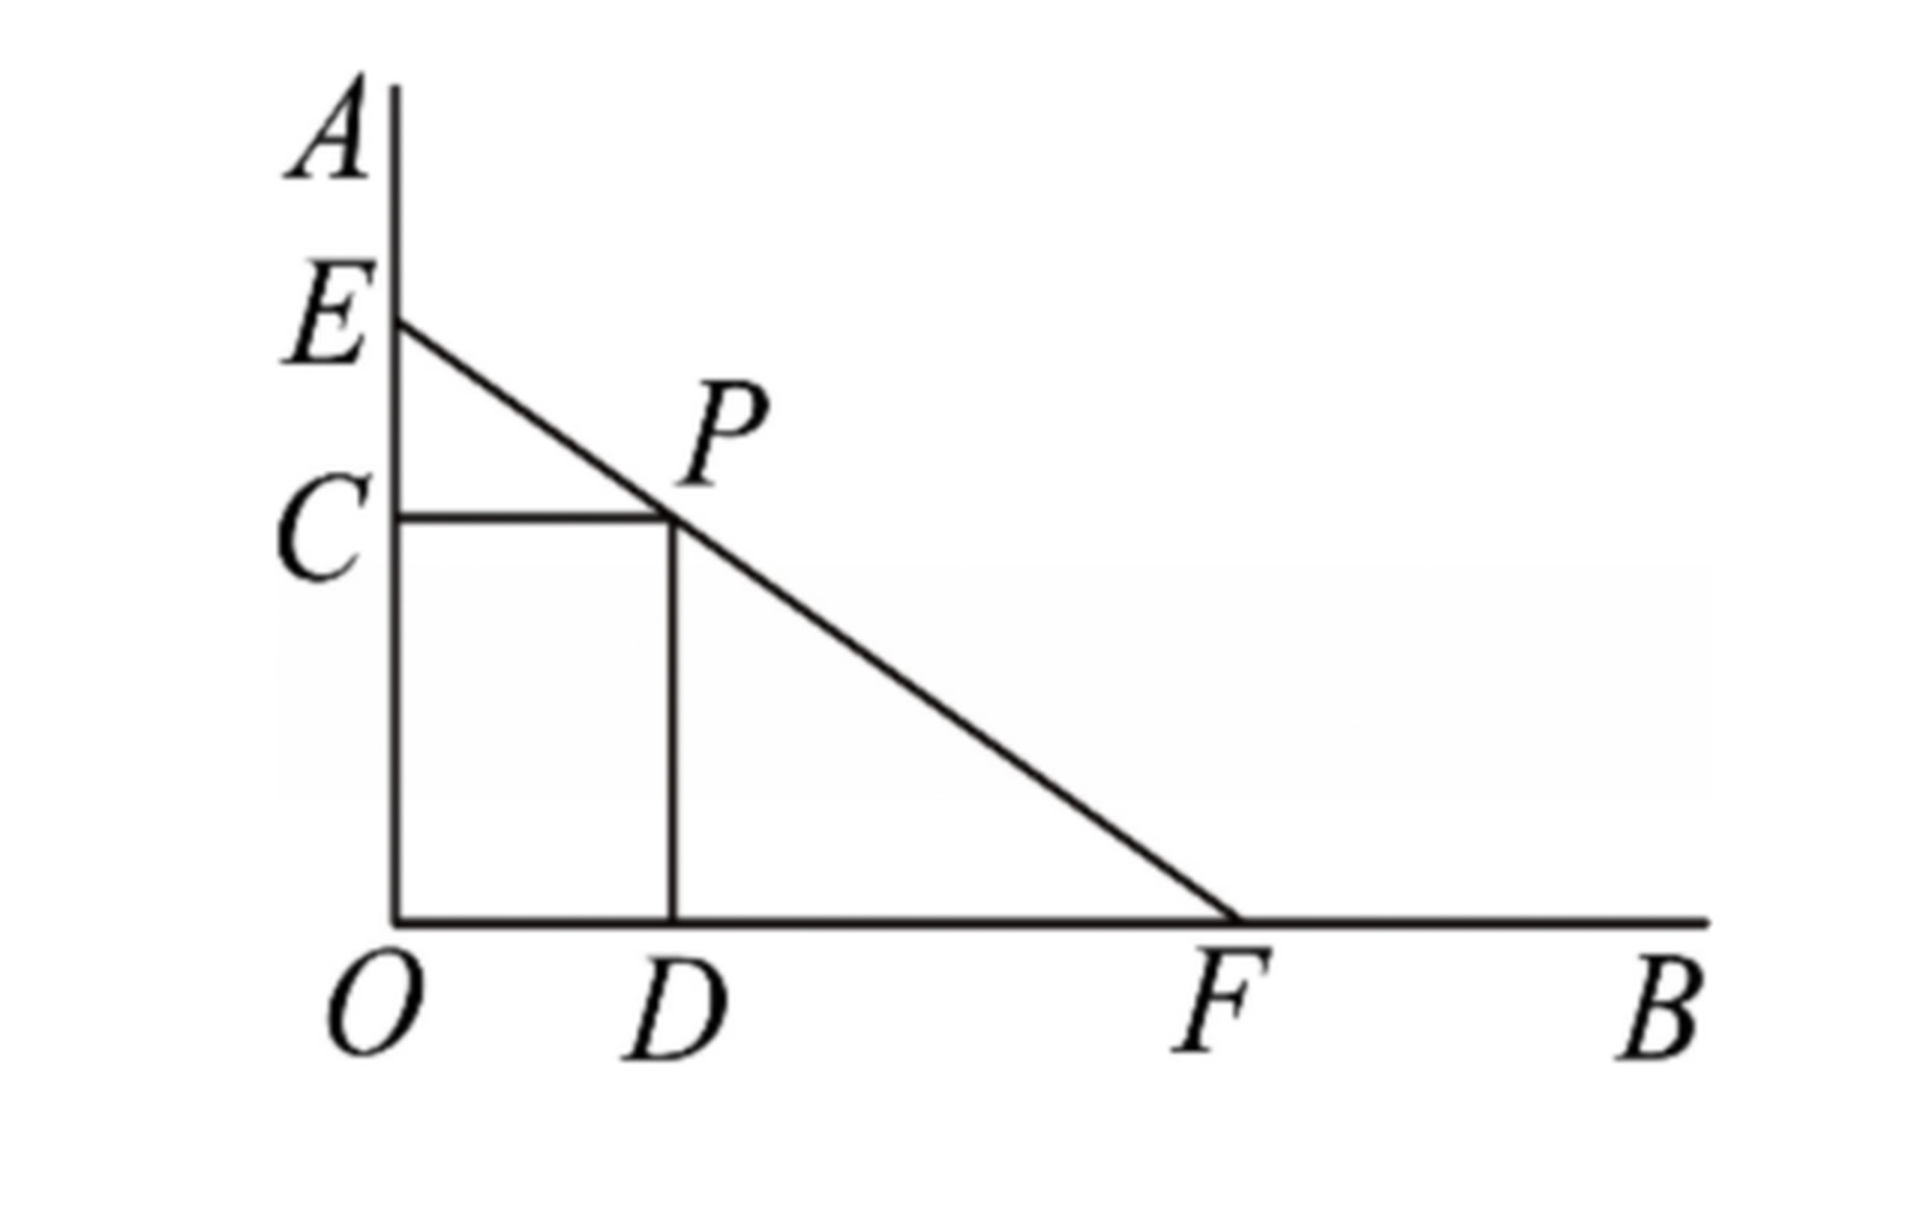
\includegraphics[width=0.32\textwidth]{figures/gao132_q18.png}
\end{center}

\ifanswer
\solbegin
\step{(1) 由题意得 $x\leq60$，}
\step{$\triangle PCE\sim\triangle FDP$，所以 $\dfrac{EC}{CP}=\dfrac{PD}{DF}$，即 $\dfrac{x}{25}=\dfrac{40}{DF}$，得 $DF=\dfrac{1000}{x}$m，}
\step{所以 $OF=OD+DF=\left(25+\dfrac{1000}x\right)$m，}
\step{所以 $25+\dfrac{1000}x\leq100$，解得 $x\geq\dfrac{40}3$；}
\step{综上，$\dfrac{40}3\leq x\leq60$；}
\step{(2) 由 $OE=OC+CE=(40+x)$m，}
\step{所以 $S=\dfrac12 OF\cdot OE=\dfrac12\left(25+\dfrac{1000}x\right)(40+x)$}
\step{$=\dfrac12\left(1000+25x+\dfrac{40000}x+1000\right)$m$^2$，}
\step{由基本不等式得 $S\geq\dfrac12\left(2000+2\sqrt{25x\cdot\dfrac{40000}x}\right)=2000$m$^2$，}
\step{当且仅当 $25x=\dfrac{40000}x$，即 $x=40$ 时取等号，}
\step{故 $EC=40$m 时，$S$ 取得最小值，为 $2000$m$^2$.}
\solend
\fi

\item 已知 $a>0$，$b>0$，请选择适当的方法证明.

(1) 若 $a\ne b$，证明：$a^3+b^3>a^2b+ab^2$；

(2) 若 $ab=1$，证明：$a^2+a<2$ 与 $b^2+b<2$ 不能同时成立.

\ifanswer
\solbegin
\step{(1) 因为 $a>0$，$b>0$，$a\ne b$，}
\step{所以 $a^3+b^3-a^2b-ab^2=a^2(a-b)+b^2(b-a)$}
\step{$=(a^2-b^2)(a-b)=(a-b)^2(a+b)>0$，所以 $a^3+b^3>a^2b+ab^2$.}
\step{(2) 假设 $a^2+a<2$ 与 $b^2+b<2$ 同时成立，所以 $-2<a<1,-2<b<1$，}
\step{又因为 $a>0,b>0$，所以 $0<a<1,0<b<1$，}
\step{所以 $0<ab<1$，这与 $ab=1$ 矛盾，}
\step{故 $a^2+a<2$ 与 $b^2+b<2$ 不可能同时成立.}
\solend
\fi

\item 若设 $M(a,n)=\lvert ax-1\rvert+\lvert ax-2\rvert+\cdots+\lvert ax-n\rvert$ 为曼哈顿扩张距离，它由 $n$ 个绝对值之和组成，其中 $n$ 为正整数.

(1) 若 $M(2,1)\leq5$，求 $x$ 的取值范围；

(2) 若 $k\leq M(2,2)$ 对一切实数 $x$ 恒成立，求实数 $k$ 的取值范围；

(3) $M(2,6)$ 是否存在最小值？若存在，求出该最小值与此时实数 $x$ 的取值范围；若不存在，说明理由.

\ifanswer
\solbegin
\step{(1) $M(2,1)=\lvert2x-1\rvert\leq5$，则不等式可化为 $-5\leq2x-1\leq5$，解得 $-2\leq x\leq3$，}
\step{所以 $x$ 的取值范围为 $[-2,3]$.}
\step{(2) 因为 $k\leq M(2,2)=\lvert2x-1\rvert+\lvert2x-2\rvert$ 对一切实数 $x$ 恒成立，}
\step{又 $\lvert2x-1\rvert+\lvert2x-2\rvert\geq\lvert(2x-1)-(2x-2)\rvert=1$，}
\step{当且仅当 $(2x-1)(2x-2)\leq0$，即 $\dfrac12\leq x\leq1$ 时取等号，}
\step{故 $k\leq1$，所以实数 $k$ 的取值范围为 $(-\infty,1]$.}
\step{(3) $M(2,6)=\lvert2x-1\rvert+\lvert2x-2\rvert+\lvert2x-3\rvert+\lvert2x-4\rvert+\lvert2x-5\rvert+\lvert2x-6\rvert$}
\step{$=2\left(\left\lvert x-\dfrac12\right\rvert+\lvert x-1\rvert+\left\lvert x-\dfrac32\right\rvert+\lvert x-2\rvert+\left\lvert x-\dfrac52\right\rvert+\lvert x-3\rvert\right)$，}
\step{其中 $\left\lvert x-\dfrac12\right\rvert+\lvert x-1\rvert+\left\lvert x-\dfrac32\right\rvert+\lvert x-2\rvert+\left\lvert x-\dfrac52\right\rvert+\lvert x-3\rvert$ 的几何意义为}
\step{在数轴上一点 $x$ 到 $\dfrac12,1,\dfrac32,2,\dfrac52,3$ 的距离之和，}
\step{要想距离之和最小，其中 $x\in\left[\dfrac12,3\right]$ 时，$\left\lvert x-\dfrac12\right\rvert+\lvert x-3\rvert$ 取得最小值，}
\step{当 $x\in\left[1,\dfrac52\right]$ 时，$\lvert x-1\rvert+\left\lvert x-\dfrac52\right\rvert$ 取得最小值，}
\step{当 $x\in\left[\dfrac32,2\right]$ 时，$\left\lvert x-\dfrac32\right\rvert+\lvert x-2\rvert$ 取得最小值，}
\step{综上，当 $x\in\left[\dfrac32,2\right]$ 时，$\left\lvert x-\dfrac12\right\rvert+\lvert x-1\rvert+\left\lvert x-\dfrac32\right\rvert+\lvert x-2\rvert+\left\lvert x-\dfrac52\right\rvert+\lvert x-3\rvert$}
\step{取得最小值，最小值为 $3-\dfrac12+\dfrac52-1+2-\dfrac32=\dfrac92$，}
\step{故 $M(2,6)=2\left(\left\lvert x-\dfrac12\right\rvert+\lvert x-1\rvert+\left\lvert x-\dfrac32\right\rvert+\lvert x-2\rvert+\left\lvert x-\dfrac52\right\rvert+\lvert x-3\rvert\right)$ 的}
\step{最小值为 $9$.}
\solend
\fi

\item 已知集合 $A=\{a_1,a_2,\cdots,a_n\}(0\leq a_1<a_2<\cdots<a_n,n\in\N,n\geq3)$ 具有性质 $Q$：对任意 $i,j(1\leq i\leq j\leq n)$，$a_i+a_j$ 与 $a_j-a_i$ 至少有一个属于集合 $A$；

(1) 判断集合 $M=\{0,2,4\}$ 与 $N=\{2,3,4\}$ 是否具有性质 $Q$，并说明理由；

(2) 已知 $A=\{a_1,a_2,a_3\}$ 具有性质 $Q$，当 $a_2=2026$ 时，求集合 $A$；

(3) 已知 $B=\{b_1,b_2,\cdots,b_{2026}\}$ 具有性质 $Q$，求 $\dfrac{b_1+b_2+\cdots+b_{2026}}{b_{2026}}$ 的值；

\ifanswer
\solbegin
\step{(1) 集合 $M=\{0,2,4\}$ 中，}
\step{因为 $0+2\in M,0+4\in M,4-2\in M,0\pm0=0\in M$，}
\step{$2+2=4\in M,2-2=0\in M,4-4=0\in M$，所以集合 $M$ 具有性质 $Q$；}
\step{集合 $N=\{2,3,4\}$ 中，因为 $3+3=6\notin N,3-3=0\notin N$，}
\step{所以集合 $N$ 不具有性质 $Q$.}
\step{(2) 因为 $a_1<a_2<a_3$，且 $A=\{a_1,a_2,a_3\}$ 具有性质 $Q$，}
\step{所以 $a_3+a_3\notin A,a_3-a_3=0\in A$，则 $a_1=0$，}
\step{又因为 $a_2+a_3>a_3$，所以 $a_2+a_3\notin A$，则 $a_3-a_2\in A$，}
\step{由集合的互异性得 $a_3-a_2=a_2$，而 $a_2=2026$，所以 $a_3=4052$，}
\step{故 $A=\{0,2026,4052\}$；}
\step{(3) 先证明一般结论：$A=\{a_1,a_2,\cdots,a_n\}(0\leq a_1<a_2<\cdots<a_n,n\in\N,n\geq3)$}
\step{具有性质 $Q$，则 $a_1+a_2+a_3+\cdots+a_n=\dfrac n2 a_n$.}
\step{因为 $A=\{a_1,a_2,\cdots,a_n\}(0\leq a_1<a_2<\cdots<a_n,n\in\N,n\geq3)$ 具有性质 $Q$，}
\step{所以 $a_n+a_n\notin A$，则 $a_n-a_n=0\in A$，则 $a_1=0$.}
\step{又因为 $0\leq a_1<a_2<\cdots<a_n$，所以 $0\leq a_n-a_n<a_n-a_{n-1}<\cdots<a_n-a_1$，}
\step{又因为 $a_n+a_{n-i}>a_n(i=1,2,\cdots,n-1)$，所以 $a_n+a_{n-i}\notin A$，}
\step{则 $a_n-a_{n-i}\in A$，}
\step{所以 $a_1=a_n-a_n,a_2=a_n-a_{n-1},a_3=a_n-a_{n-2},\cdots,a_n=a_n-a_1$.}
\step{所以 $a_1+a_2+a_3+\cdots+a_n$}
\step{$=(a_n-a_n)+(a_n-a_{n-1})+(a_n-a_{n-2})+\cdots+(a_n-a_1)$，}
\step{即 $a_1+a_2+a_3+\cdots+a_n=\dfrac n2 a_n$，}
\step{所以 $B=\{b_1,b_2,\cdots,b_{2026}\}$ 具有性质 $Q$，则 $b_1+b_2+\cdots+b_{2026}=\dfrac{2026}{2}b_{2026}$，}
\step{所以 $\dfrac{b_1+b_2+\cdots+b_{2026}}{b_{2026}}=\dfrac{2026}{2}=1013$.}
\solend
\fi

\end{enumerate}

% 行数复核：逐题数 \step 条数，合计 144 条（Q3：4；Q4：1；Q5：4；Q6：2；Q7：9；Q8：2；
% Q9：3；Q10：6；Q11：9；Q12：9；Q13：0；Q14：9；Q15：4；Q16：19；Q17：5；Q18：11；
% Q19：7；Q20：17；Q21：23），与原卷印刷行逐题相等（cases 块作一个印刷行计）。
% 第 13 题只印括号内答案、提 \ans{}，不计入 \step 账；第 14—16 题答案在解析末句，
% 括号内留空、不另提 \ans{}。

\end{document}
"
%
% 原始材料：微信公众号"魔都数学加油站"文章，作者破晓，2026-11-14 19:00 发布；
% 连载"27学年高一132"，原文标题"27学年高一132——2026-2027年上海市川沙中学高一上期中"；
% 原文链接：https://mp.weixin.qq.com/s/VBG01CrUNMIYWWHhSfz8JQ。
% 正文为 11 张 PNG 页（01、04、06、07、09、11 为 2560x3620，02、03、05、08、10 为 4762x6735），
% 题目下印有【解析】，为讲评版。题目、解析均据原图转录；
% 卷面粉红色水印"魔都数学加油站"及公众号页脚未录入。全卷 2 幅插图：第 14 题四幅坐标图选项、
% 第 18 题矩形 OCPD 与小路 EF 示意图，均取原卷 04／07 页截图去水印。
%
% 卷首标题：原卷印作"2026-2027 年川沙中学高一上期中"（公众号标题中的"上海市"
% 卷面标题行没有，本稿照卷面），年份区间按全稿惯例排 en dash；原卷未印副标题，
% 本卷为期中卷、跨集合与常用逻辑用语／不等式／函数三章，按题目内容标为
% "集合与常用逻辑用语、不等式、函数"（与 125／126／128／129／131 同期中卷口径相同）：
% 集合与逻辑见 Q5、Q6、Q17、Q21，不等式见 Q3、Q4、Q9、Q10、Q12、Q13、Q15、Q16、Q19，
% 函数（幂函数、指数／对数、基本不等式应用）见 Q7、Q8、Q11、Q14、Q18、Q20。
%
% 题号体例：本卷共 19 题——一、填空题 3—12（10 题）、二、选择题 13—16（4 题）、
% 三、解答题 17—21（5 题）。三节分别 \setcounter{enumi}{2}／{12}／{16}。
%
% 与原卷的排版差异：
%   ① 原文从第 3 题起，本稿保留原题号（见上"题号体例"）；
%   ② 原卷每题下直接印【解析】，本稿按全稿惯例置于答案版；第 13 题答案 D 印在题干
%      括号内、无独立答案段，按 高一37／52／53／55／63／64／128／131 成例括号留空、
%      另提 \ans{$D$}；第 14—16 题答案在解析末句"故选 …"，括号内留空、不另提 \ans{}；
%   ③ 原卷未印副标题，本稿按"知识模块"口径补出；
%   ④ 原卷填空横线按全稿惯例排为 \blankline[4.4em]；选择题括号排 \mbox{（\quad）}、
%      选项段前按惯例加 \keepwithprev；解答题不留作答区（原卷为讲评版，与 109—131 同）；
%   ⑤ 原卷数集排斜体 $R^+$／$R$／$Z$／$N$，按全稿惯例改 \R^+／\R／\Z／\N；
%      绝对值排 \lvert…\rvert，集合描述竖线排 \mid；不等号按全稿惯例排 \leqslant／\geqslant；
%      补集照原卷上划线排 \overline{B}；
%   ⑥ 子题标号 (1)(2)(3) 原卷用半角括号，照录；第 14 题四幅坐标图选项按原卷 2×2 排布
%      合并裁为一张 \includegraphics（未用 TikZ 重绘，以保证与原卷一致），题前加
%      \needvspace{9cm} 守卫；第 18 题图取 07 页截图，题前按惯例加 \needvspace{7cm} 守卫
%      （照 高一120／127／129／131 成例），两者守卫都放在 \item 之前；
%   ⑦ 原卷 Q7 解析跨 01—02 页、Q10 解析跨 02—03 页、Q12 解析跨 03—04 页、
%      Q14 解析跨 04—05 页、Q16 解析在 06 页、Q18 解析跨 07—08 页、
%      Q20 解析跨 08—09 页、Q21 解析跨 10—11 页，本稿按题合并连续排版；
%      末页第 11 页为 Q21 (3) 解析的续尾，按实际印刷行单列。
%
% 判别式字形：第 10 题 $\triangle=4(a-1)^2+16(a-1)<0$、第 11 题
%   $\triangle=4(m-2)^2-4(m^2-3m+3)=-4m+4>0$ 两处原卷均排 $\triangle$（等边、扁），
%   逐处放大核对、字形一致，照录 \triangle；与 高一129／131 同题排 $\Delta$（等腰、高）不同。
%   全卷 \triangle 兼作第 18 题「$\triangle PCE\sim\triangle FDP$」「$\triangle OEF$」的几何
%   三角形记号，全卷未出现 \Delta。
%
% 子集符号：第 5 题解析 $B\subseteq A$、第 17 题 (2) 解析 $A\subseteq B$ 均印带下划线，
%   照录 \subseteq；全卷未出现单线 \subset。
%
% 原卷存疑照录：
%   第 9 题题干作"充分非必要条件"、解析作"充分不必要条件"，措辞不同，照录；
%   第 10 题解析"当 $a-1=0$ 时，$-4\geq0$，不等式不成立，$a=1$ 满足题意"照录；
%   第 11 题解析"所以 $2(m-1)+\dfrac1{m-1}\leq-2\sqrt2$"由上一行 $2(1-m)+\dfrac1{1-m}\geq2\sqrt2$
%     直接变号得到，照录；
%   第 12 题解析"由 $x\in Z$，$-7<-2\sqrt{10}<-6$"与"即 $k^2+7k+10\leq0$，解得 $-5\leq k\leq-2$"照录；
%   第 16 题解析"令 $52\times(930+a)=-52$，解得 $a=-931$"（按式应为 $a=-931$ 之外的解）照录；
%   第 19 题 (2) 解析"所以 $-2<a<1,-2<b<1$"数学式内半角逗号，照录；
%   第 20 题 (3) 解析"最小值为 $3-\dfrac12+\dfrac52-1+2-\dfrac32=\dfrac92$"与
%     "故 $M(2,6)=\dots$ 的最小值为 9"两处结论并列，照录；
%   第 21 题 (1) 解析"$0+2\in M,0+4\in M,4-2\in M,0\pm0=0\in M$"、
%     "$2+2=4\in M,2-2=0\in M,4-4=0\in M$"、(3) 各连写等式内半角逗号，照录；
%   第 21 题 (3) 解析"即 $a_1+a_2+a_3+\cdots+a_n=\dfrac n2 a_n$，"句末用半角逗号，照录。
%
% 行数复核：见文末"行数复核"注（逐题 \step 条数与原卷印刷行逐题相等，cases 块作一个印刷行计）。
%   第 13 题只印括号内答案、提 \ans{}，不计入 \step 账；第 14—16 题答案在解析末句，
%   括号内留空、不另提 \ans{}。
%
\documentclass[a4paper,11pt]{article}
\usepackage{common}

\begin{document}

\examtitlest[3]{2026--2027 年川沙中学高一上期中}{集合与常用逻辑用语、不等式、函数}

\bigsec{一、填空题}

\begin{enumerate}
\setcounter{enumi}{2}

\item 已知 $a$、$b\in\R^+$ 且 $ab=2$，则 $a+2b$ 的最小值为\blankline[4.4em].

\ifanswer
\solbegin
\step{因为 $a\in\R^+$，$b\in\R^+$ 且 $ab=2$，}
\step{由基本不等式得 $a+2b\geq2\sqrt{a\cdot2b}=2\sqrt{2ab}=2\sqrt4=4$.}
\step{等号当且仅当 $a=2b$ 时成立，结合 $ab=2$ 解得 $b=1$，$a=2$，}
\step{所以 $a+2b$ 的最小值为 $4$.}
\solend
\fi

\item 如果幂函数 $f(x)=(m^2-3m-3)x^{m^2+m-3}$ 在 $(0,+\infty)$ 上是增函数，则实数 $m=$\blankline[4.4em].

\ifanswer
\solbegin
\step{由已知得 $\begin{cases}m^2-3m-3=1\\m^2+m-3>0\end{cases}$，所以 $m=4$.}
\solend
\fi

\item 已知集合 $A=\{1,2\}$，集合 $B=\{x\mid ax=6\}$，若 $A\cup B=A$，则 $a$ 的所有取值构成的集合为\blankline[4.4em].

\ifanswer
\solbegin
\step{因为 $A\cup B=A$，所以 $B\subseteq A$，}
\step{当 $a=0$ 时，$B=\varnothing$，满足 $B\subseteq A$；}
\step{当 $a\ne0$ 时，$B=\left\{\dfrac6a\right\}$，则 $\dfrac6a=1$ 或 $\dfrac6a=2$，解得 $a=6$ 或 $a=3$，}
\step{综上所述，$a$ 的所有取值构成的集合为 $\{0,3,6\}$.}
\solend
\fi

\item 设全集为 $\R$，$A=\{y\mid y=-x^2+2x+1\}$，$B=\{x\mid y=\ln(x-1)\}$，则 $A\cap B=$\blankline[4.4em].

\ifanswer
\solbegin
\step{$A=\{y\mid y=-x^2+2x+1\}=\{y\mid y=-(x-1)^2+2\}=\{y\mid y\leq2\}$，}
\step{$B=\{x\mid y=\ln(x-1)\}=\{x\mid x>1\}$，则 $A\cap B=(1,2]$.}
\solend
\fi

\item 已知 $x\in\R$，则方程 $\lvert 6-x\rvert+\lvert 6x-3\rvert=\lvert 5x+3\rvert$ 的解集为\blankline[4.4em].

\ifanswer
\solbegin
\step{当 $x<-\dfrac35$ 时，$6-x>0$，$6x-3<0$，$5x+3<0$，}
\step{原方程为 $6-x-6x+3=-5x-3$，解得 $x=6$，不满足 $x<-\dfrac35$；}
\step{当 $-\dfrac35\leq x\leq\dfrac12$ 时，$5x+3\geq0$，$6x-3<0$，$6-x>0$，}
\step{原方程为 $6-x+3-6x=5x+3$，解得 $x=\dfrac12$；}
\step{当 $\dfrac12<x\leq6$ 时，$5x+3>0$，$6x-3>0$，$6-x\geq0$，}
\step{原方程为 $6-x+6x-3=5x+3$，即 $0=0$，恒成立，所以 $\dfrac12<x\leq6$；}
\step{当 $x>6$ 时，$5x+3\geq0$，$6x-3>0$，$6-x<0$，}
\step{原方程为 $x-6+6x-3=5x+3$，解得 $x=6$，不满足 $x>6$；}
\step{综上 $\dfrac12\leq x\leq6$，所以原方程的解集为 $\left\{x\mid\dfrac12\leq x\leq6\right\}$.}
\solend
\fi

\item 已知 $\log_2 3=a,2^b=7$，用 $a,b$ 表示 $\log_{42}56$ 为\blankline[4.4em].

\ifanswer
\solbegin
\step{$\log_{42}56=\dfrac{\log_2 56}{\log_2 42}=\dfrac{\log_2(7\times8)}{\log_2(6\times7)}=\dfrac{\log_2 7+\log_2 8}{\log_2 6+\log_2 7}$}
\step{$=\dfrac{\log_2 7+\log_2 2^3}{\log_2 2+\log_2 3+\log_2 7}=\dfrac{b+3}{1+a+b}$.}
\solend
\fi

\item 已知 $\dfrac13<x<\dfrac12$ 是不等式 $\lvert x-m\rvert<1$ 成立的充分非必要条件，则 $m$ 的取值范围是\blankline[4.4em].

\ifanswer
\solbegin
\step{因为 $\lvert x-m\rvert<1$，所以 $-1<x-m<1$，所以 $m-1<x<m+1$，}
\step{所以 $m-1<x<m+1$ 成立的充分不必要条件是 $\dfrac13<x<\dfrac12$，}
\step{所以 $\begin{cases}m-1\leq\dfrac13\\m+1\geq\dfrac12\end{cases}$，解得 $-\dfrac12\leq m\leq\dfrac43$，故 $m$ 的取值范围是 $\left[-\dfrac12,\dfrac43\right]$.}
\solend
\fi

\item 若关于 $x$ 的不等式 $(a-1)x^2+2(a-1)x-4\geq0$ 的解集为空集，则 $a$ 的取值范围是\blankline[4.4em].

\ifanswer
\solbegin
\step{关于 $x$ 的不等式 $(a-1)x^2+2(a-1)x-4\geq0$ 的解集为 $\varnothing$，}
\step{当 $a-1=0$ 时，$-4\geq0$，不等式不成立，$a=1$ 满足题意；}
\step{当 $a-1>0$ 时，$a>1$，不等式的解集不为空集，不满足题意；}
\step{当 $a-1<0$ 时，$a<1$，当 $\triangle=4(a-1)^2+16(a-1)<0$ 时，即 $(a-1)(a+3)<0$，}
\step{解得 $-3<a<1$，满足题意；}
\step{综上，实数 $a$ 的取值范围是 $\{a\mid-3<a\leq1\}$.}
\solend
\fi

\item 已知关于 $x$ 的方程 $x^2+2(m-2)x+m^2-3m+3=0$ 有两个不相等的实数根 $x_1$、$x_2$，则 $\dfrac{mx_1}{x_1-1}+\dfrac{mx_2}{x_2-1}-\dfrac{2}{x_1+x_2-2}$ 的最大值为\blankline[4.4em].

\ifanswer
\solbegin
\step{关于 $x$ 的方程 $x^2+2(m-2)x+m^2-3m+3=0$ 有两个不相等的实数根 $x_1$、$x_2$，}
\step{则 $\triangle=4(m-2)^2-4(m^2-3m+3)=-4m+4>0$，得 $m<1$，}
\step{且 $x_1+x_2=-2(m-2)$，$x_1x_2=m^2-3m+3$，}
\step{$\dfrac{mx_1}{x_1-1}+\dfrac{mx_2}{x_2-1}-\dfrac{2}{x_1+x_2-2}=\dfrac{m[2x_1x_2-(x_1+x_2)]}{x_1x_2-(x_1+x_2)+1}+\dfrac1{m-1}$}
\step{$=\dfrac{2m(m-1)^2}{m^2-m}+\dfrac1{m-1}=2(m-1)+\dfrac1{m-1}$，}
\step{又因为 $m<1$，所以 $m-1<0$，则 $1-m>0$，}
\step{所以 $2(1-m)+\dfrac1{1-m}\geq2\sqrt{2(1-m)\cdot\dfrac1{1-m}}=2\sqrt2$，}
\step{当且仅当 $2(1-m)=\dfrac1{1-m}$ 时，即 $m=1-\dfrac{\sqrt2}2$ 时取等号，}
\step{所以 $2(m-1)+\dfrac1{m-1}\leq-2\sqrt2$，即 $\dfrac{mx_1}{x_1-1}+\dfrac{mx_2}{x_2-1}-\dfrac2{x_1+x_2-2}$ 的最大值为 $-2\sqrt2$.}
\solend
\fi

\item 若使集合 $A=\{x\mid(kx-k^2-10)(x-1)>0,x\in\Z\}$ 中的元素个数最少，则实数 $k$ 的取值范围是\blankline[4.4em].

\ifanswer
\solbegin
\step{由题意集合 $A=\{x\mid(kx-k^2-10)(x-1)>0,\ x\in\Z\}$，}
\step{$k=0$ 时，不等式解得 $x<1$，有无数个整数解；}
\step{$k\ne0$ 时，则不等式变形为 $k\left(x-k-\dfrac{10}k\right)(x-1)>0$，}
\step{当 $k>0$ 时，$k+\dfrac{10}k\geq2\sqrt{10}$，仅当 $k=\sqrt{10}$ 时等号成立，}
\step{此时不等式解得 $x>k+\dfrac{10}k$ 或 $x<1$，有无数个整数解；}
\step{当 $k<0$ 时，$k+\dfrac{10}k=-\left[(-k)+\left(-\dfrac{10}k\right)\right]\leq-2\sqrt{10}$，仅当 $k=-\sqrt{10}$ 时等号成立，}
\step{此时不等式解得 $k+\dfrac{10}k<x<1$，}
\step{由 $x\in\Z$，$-7<-2\sqrt{10}<-6$，要使集合 $A$ 中的元素最少，则 $k+\dfrac{10}k\geq-7$，}
\step{即 $k^2+7k+10\leq0$，解得 $-5\leq k\leq-2$，故实数 $k$ 的取值范围是 $[-5,-2]$.}
\solend
\fi

\end{enumerate}

\bigsec{二、选择题}

\begin{enumerate}
\setcounter{enumi}{12}

\item 下列说法正确的是\mbox{（\quad）}

\keepwithprev
A. 若 $a>b$，则 $\dfrac1a<\dfrac1b$\qquad\qquad B. 若 $a>b$，$c>d$，则 $ac>bd$

C. 若 $a>b$，则 $ac^2>bc^2$\qquad\qquad D. 若 $ac^2>bc^2$，则 $a>b$

\ifanswer
\ans{$D$}
\fi

% 第 14 题四幅坐标图选项是一整块，守卫放在 \item 之前
\needvspace{9cm}
\item 在同一坐标系内，函数 $y=x^a(a\ne0)$ 和 $y=ax-\dfrac1a$ 的图象可能是\mbox{（\quad）}

\keepwithprev
\begin{center}
% 四幅坐标图选项取原卷 04 页截图去粉色水印，按原卷 2×2 排布合并为一张
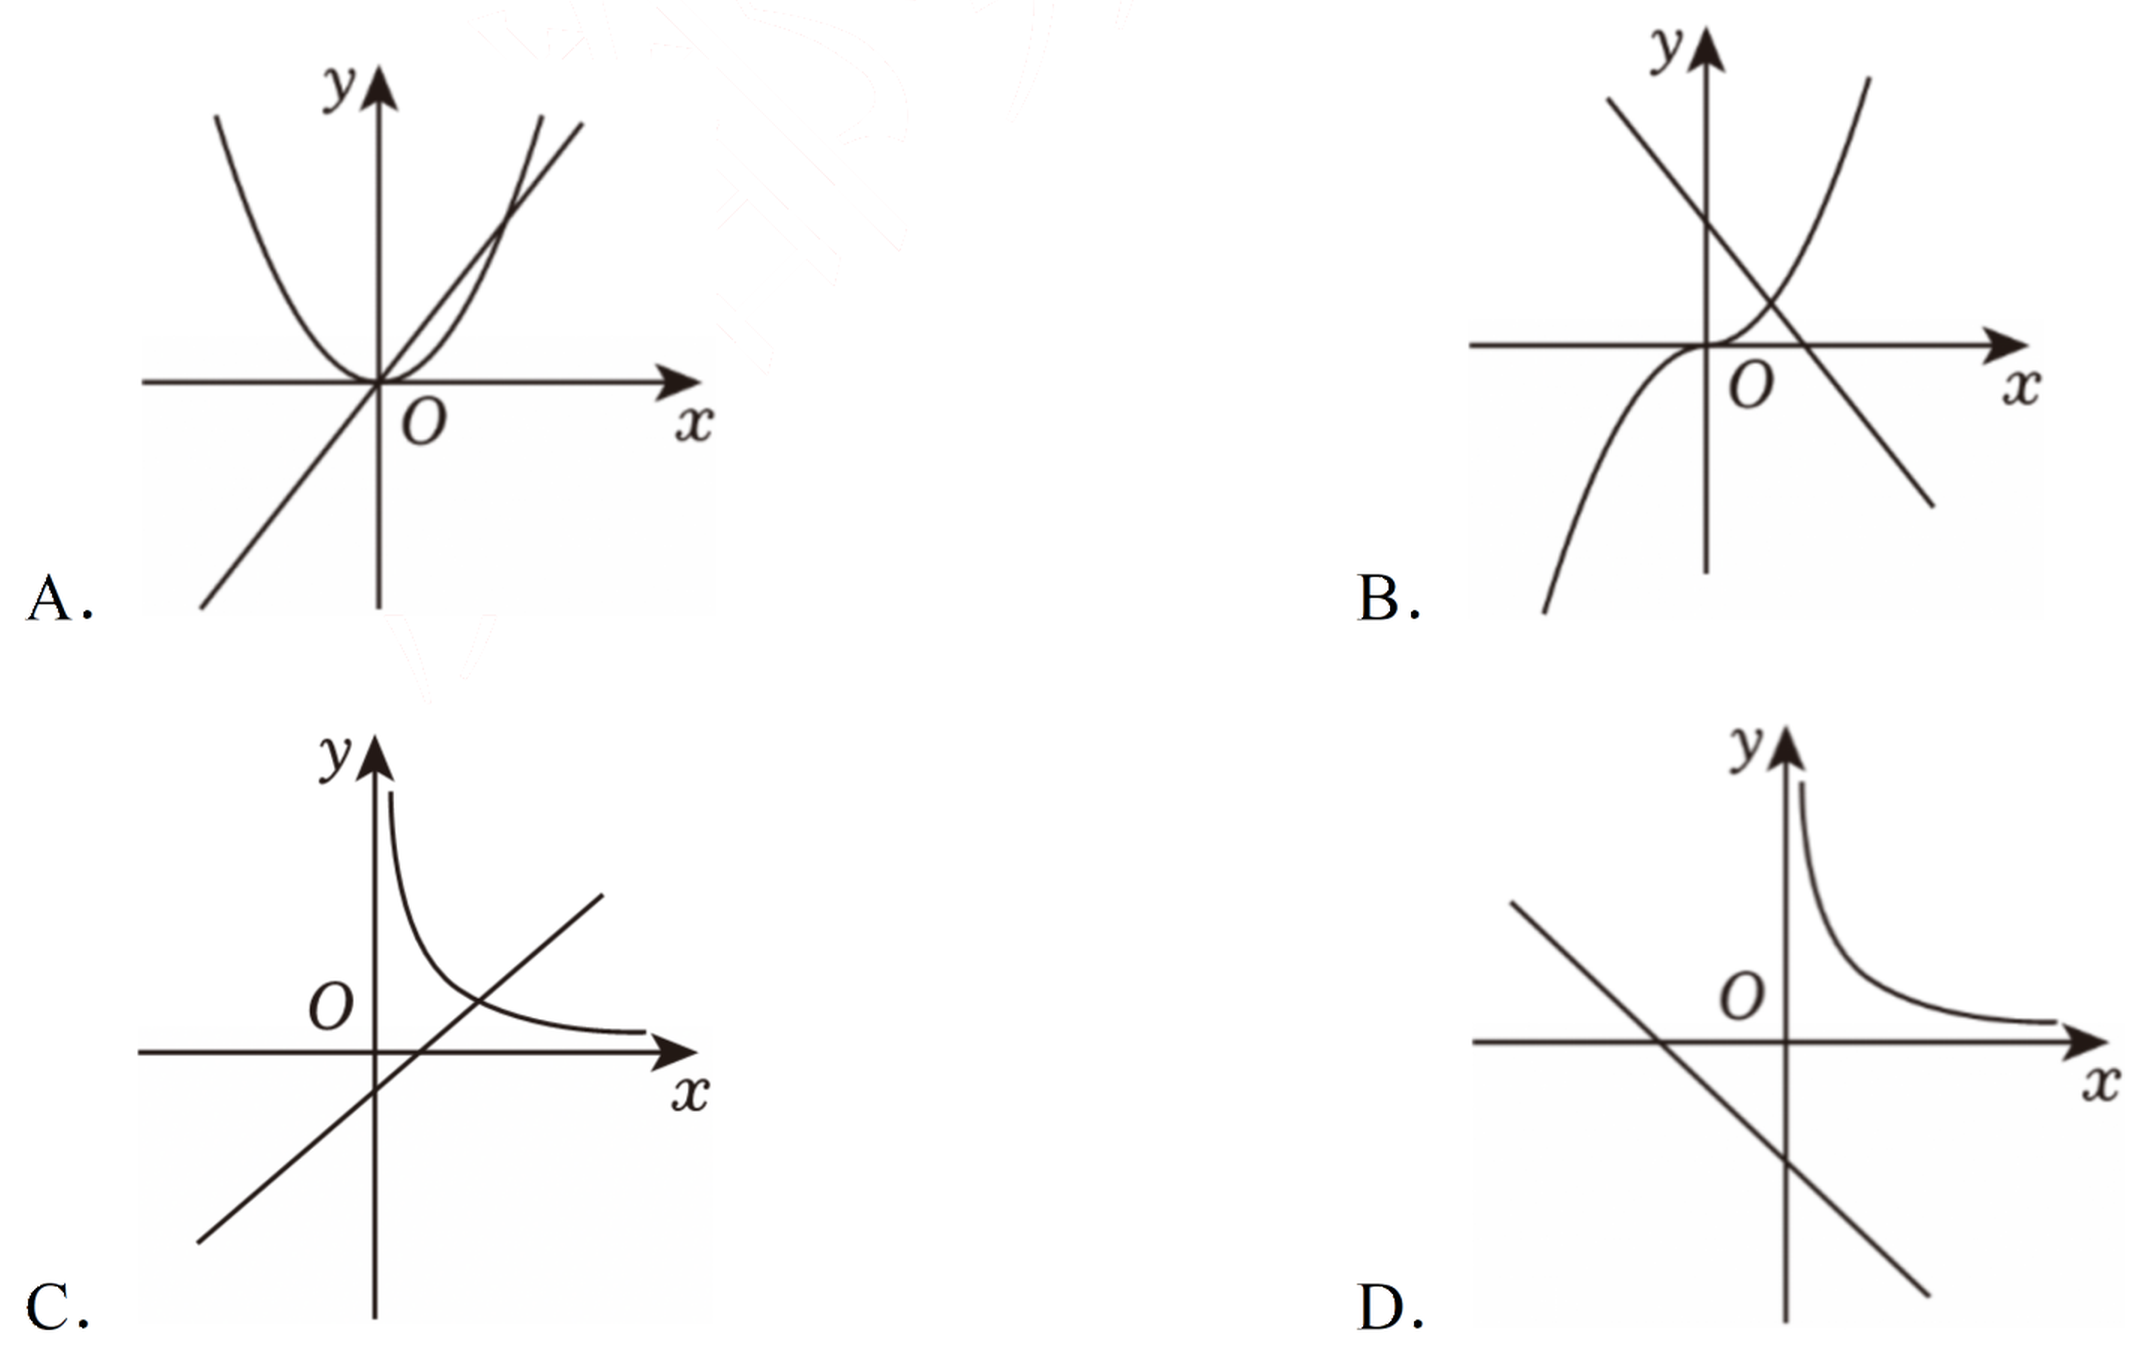
\includegraphics[width=0.80\textwidth]{figures/gao132_q14.png}
\end{center}

\ifanswer
\solbegin
\step{当 $a>0$ 时，$y=ax-\dfrac1a$ 严格增，当 $a<0$ 时，$y=ax-\dfrac1a$ 严格减，}
\step{对于 $A$，因为 $a\ne0$，所以直线 $y=ax-\dfrac1a$ 不过原点，故 $A$ 错误；}
\step{对于 $B$，由函数 $y=x^a(a\ne0)$ 的图象得 $a>1$，}
\step{由 $y=ax-\dfrac1a$ 的图象得 $a<0$，互相矛盾，故 $B$ 错误；}
\step{对于 $C$，由函数 $y=x^a(a\ne0)$ 的图象得 $a>1$，}
\step{由 $y=ax-\dfrac1a$ 的图象得 $a>0$ 且 $-\dfrac1a<0$，符合题意，故 $C$ 正确；}
\step{对于 $D$，由函数 $y=x^a(a\ne0)$ 的图象得 $a<0$，}
\step{由 $y=ax-\dfrac1a$ 的图象得 $a<0$ 且 $-\dfrac1a<0$，互相矛盾，故 $D$ 错误；}
\step{故选 $C$.}
\solend
\fi

\item 中国的 $5G$ 技术领先世界，在 $5G$ 技术中，最大数据传输速率 $C$ 取决于信道带宽 $W$，$C$ 与 $W$ 满足 $C=W\log_2\left(1+\dfrac SN\right)$，其中 $\dfrac SN$ 称为信噪比（单位：$dB$）. 若不改变带宽 $W$，初始信噪比 $\dfrac SN$ 为 $1000$，那么为了使 $C$ 增加 $30\%$，需要将信噪比 $\dfrac SN$ 从 $1000$ 提升至大约\mbox{（\quad）}

\keepwithprev
A. $5000$\qquad\qquad B. $6000$\qquad\qquad C. $7000$\qquad\qquad D. $8000$

\ifanswer
\solbegin
\step{由题意得 $\dfrac SN=1000$ 时，$C=W\log_2(1+1000)\approx W\log_2 1000$，}
\step{要使 $C$ 增加 $30\%$，则 $(1+30\%)C=W\log_2\left(1+\dfrac SN\right)$，即 $1.3C\approx W\log_2\dfrac SN$，}
\step{所以 $1.3\approx\log_{1000}\dfrac SN=\dfrac{\lg\frac SN}{\lg1000}$，所以 $\lg\dfrac SN=3.9$，所以 $\dfrac SN=10^{3.9}\approx8000$.}
\step{故选 $D$.}
\solend
\fi

\item 对于 $a\in\R$，设非空集合 $A=\left\{x\mid\dfrac{(x^2-930x+a)(x-52)}{x+a}=0\right\}$，记 $A$ 中的所有元素之和为 $S(a)$，所有元素之积为 $T(a)$，则下列说法中，不正确的是\mbox{（\quad）}

\keepwithprev
A. 存在实数 $a$，使得 $S(a)=930$

B. 存在实数 $a$，使得 $T(a)=517$

C. 不存在实数 $a$，使得 $T(a)=0$

D. 恰存在 $1$ 个实数 $a$，使得 $T(a)=-52$

\ifanswer
\solbegin
\step{由分式值为 $0$，得分子为 $0$ 且分母不为 $0$，}
\step{分子 $(x^2-930x+a)(x-52)=0$ 的根为 $x=52$}
\step{及方程 $x^2-930x+a=0$ 的两根 $x_1$，$x_2$，}
\step{由根与系数的关系得 $x_1+x_2=930$，$x_1\cdot x_2=a$，}
\step{分母限制 $x\ne-a$，需要剔除等于 $-a$ 的根，}
\step{选项 $A$，取 $a=-52$，$x=52$ 为增根舍去，集合 $A=\{x_1,x_2\}$，}
\step{元素之和 $S(a)=930$，故 $A$ 正确；}
\step{选项 $B$，当无增根时，$T(a)=52a$，令 $52a=517$，得 $a=\dfrac{517}{52}$，}
\step{验证无增根，存在这样的 $a$，故 $B$ 正确；}
\step{选项 $C$，若 $T(a)=0$，则 $0\in A$，代入分子得 $a=0$，}
\step{但 $a=0$ 时分母 $x\ne0$，$x=0$ 为增根，$0$ 不能属于集合 $A$，}
\step{故不存在 $a$ 使得 $T(a)=0$，故 $C$ 正确；}
\step{选项 $D$，当无增根时，令 $52a=-52$，得 $a=-1$；}
\step{当 $x=-a$ 是二次方程的根且不等于 $52$ 时，}
\step{令 $52\times(930+a)=-52$，解得 $a=-931$，验证符合条件；}
\step{当 $a=-52$ 时，$x=52$，舍去，}
\step{集合 $A=\{x_1,x_2\}$，$T(a)=a=-52$，得到两个满足条件的 $a$；}
\step{因此存在 $3$ 个满足条件的 $a$，故 $D$ 错误.}
\step{故选 $D$.}
\solend
\fi

\end{enumerate}

\bigsec{三、解答题}

\begin{enumerate}
\setcounter{enumi}{16}

\item 已知全集 $U=\R$，集合 $A=\left\{x\mid\dfrac{x}{x-3}<0\right\}$，$B=\{x\mid(x-a)(x+4-a)<0\}$.

(1) 当 $a=2$ 时，求 $\overline{B}$、$A\cap\overline{B}$；

(2) 若 $A\cap B=A$，求实数 $a$ 的取值范围.

\ifanswer
\solbegin
\step{(1) $\dfrac{x}{x-3}<0$，即 $x(x-3)<0$，解得 $A=\{x\mid0<x<3\}$，}
\step{当 $a=2$ 时，$B=\{x\mid(x-a)(x+4-a)<0\}=\{x\mid-2<x<2\}$，}
\step{则 $\overline{B}=\{x\mid x\leq-2$ 或 $x\geq2\}$，故 $A\cap\overline{B}=\{x\mid2\leq x<3\}$；}
\step{(2) $A\cap B=A$，则 $A\subseteq B$，故 $\begin{cases}a-4\leq0\\a\geq3\end{cases}$，解得 $3\leq a\leq4$，}
\step{故实数 $a$ 的取值范围是 $\{a\mid3\leq a\leq4\}$.}
\solend
\fi

% 第 18 题是"题干 + 图"约 7cm 的一整块，守卫放在 \item 之前
\needvspace{7cm}
\item 如图，$OA$、$OB$ 是两条长度足够长的互相垂直的笔直小路，矩形 $OCPD$ 的顶点 $C$、$D$ 分别在 $OA$、$OB$ 上，且该矩形区域内种满了荷花. 为了让观赏者有更好的观赏体验，现计划经过点 $P$ 修一条小路 $EF$，其中点 $E$ 在小路 $OA$ 上，点 $F$ 在小路 $OB$ 上，并在 $\triangle OEF$ 区域内种满荷花. 已知 $OD=25m$，$OC=40m$，且小路 $EF$ 要完全位于一个以 $O$ 为顶点的，边长为 $100$ m 的正方形内部（包括边界）. 记 $\triangle OEF$ 的面积为 $S$m$^2$.

(1) 设 $EC=x\cdot m$，试用 $x$ 表示 $OF$，并求 $x$ 的取值范围.

(2) 当 $EC$ 的长度为多少时，$S$ 取得最小值？最小值是多少？

\begin{center}
% 图取原卷 07 页截图去粉色水印，3× LANCZOS 放大
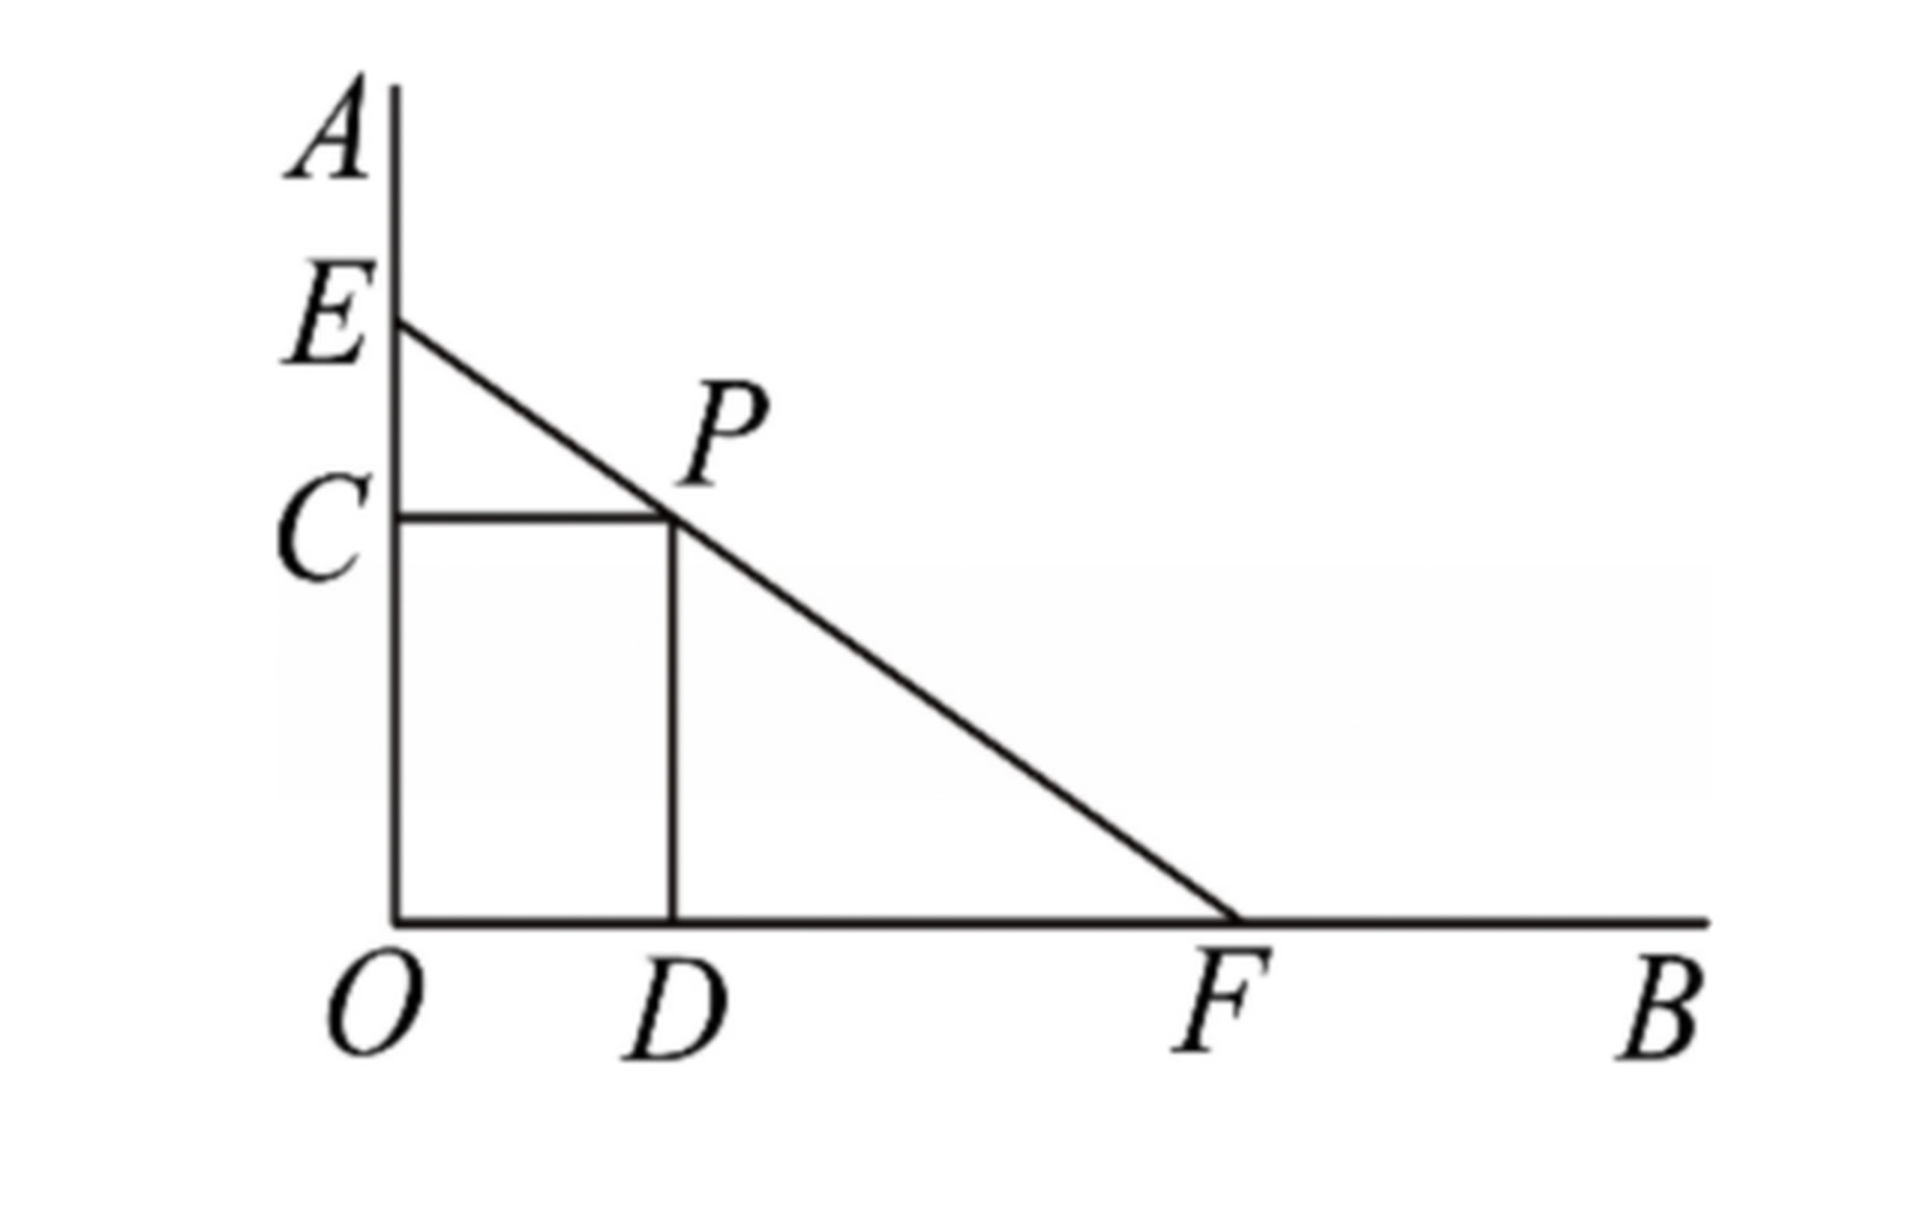
\includegraphics[width=0.32\textwidth]{figures/gao132_q18.png}
\end{center}

\ifanswer
\solbegin
\step{(1) 由题意得 $x\leq60$，}
\step{$\triangle PCE\sim\triangle FDP$，所以 $\dfrac{EC}{CP}=\dfrac{PD}{DF}$，即 $\dfrac{x}{25}=\dfrac{40}{DF}$，得 $DF=\dfrac{1000}{x}$m，}
\step{所以 $OF=OD+DF=\left(25+\dfrac{1000}x\right)$m，}
\step{所以 $25+\dfrac{1000}x\leq100$，解得 $x\geq\dfrac{40}3$；}
\step{综上，$\dfrac{40}3\leq x\leq60$；}
\step{(2) 由 $OE=OC+CE=(40+x)$m，}
\step{所以 $S=\dfrac12 OF\cdot OE=\dfrac12\left(25+\dfrac{1000}x\right)(40+x)$}
\step{$=\dfrac12\left(1000+25x+\dfrac{40000}x+1000\right)$m$^2$，}
\step{由基本不等式得 $S\geq\dfrac12\left(2000+2\sqrt{25x\cdot\dfrac{40000}x}\right)=2000$m$^2$，}
\step{当且仅当 $25x=\dfrac{40000}x$，即 $x=40$ 时取等号，}
\step{故 $EC=40$m 时，$S$ 取得最小值，为 $2000$m$^2$.}
\solend
\fi

\item 已知 $a>0$，$b>0$，请选择适当的方法证明.

(1) 若 $a\ne b$，证明：$a^3+b^3>a^2b+ab^2$；

(2) 若 $ab=1$，证明：$a^2+a<2$ 与 $b^2+b<2$ 不能同时成立.

\ifanswer
\solbegin
\step{(1) 因为 $a>0$，$b>0$，$a\ne b$，}
\step{所以 $a^3+b^3-a^2b-ab^2=a^2(a-b)+b^2(b-a)$}
\step{$=(a^2-b^2)(a-b)=(a-b)^2(a+b)>0$，所以 $a^3+b^3>a^2b+ab^2$.}
\step{(2) 假设 $a^2+a<2$ 与 $b^2+b<2$ 同时成立，所以 $-2<a<1,-2<b<1$，}
\step{又因为 $a>0,b>0$，所以 $0<a<1,0<b<1$，}
\step{所以 $0<ab<1$，这与 $ab=1$ 矛盾，}
\step{故 $a^2+a<2$ 与 $b^2+b<2$ 不可能同时成立.}
\solend
\fi

\item 若设 $M(a,n)=\lvert ax-1\rvert+\lvert ax-2\rvert+\cdots+\lvert ax-n\rvert$ 为曼哈顿扩张距离，它由 $n$ 个绝对值之和组成，其中 $n$ 为正整数.

(1) 若 $M(2,1)\leq5$，求 $x$ 的取值范围；

(2) 若 $k\leq M(2,2)$ 对一切实数 $x$ 恒成立，求实数 $k$ 的取值范围；

(3) $M(2,6)$ 是否存在最小值？若存在，求出该最小值与此时实数 $x$ 的取值范围；若不存在，说明理由.

\ifanswer
\solbegin
\step{(1) $M(2,1)=\lvert2x-1\rvert\leq5$，则不等式可化为 $-5\leq2x-1\leq5$，解得 $-2\leq x\leq3$，}
\step{所以 $x$ 的取值范围为 $[-2,3]$.}
\step{(2) 因为 $k\leq M(2,2)=\lvert2x-1\rvert+\lvert2x-2\rvert$ 对一切实数 $x$ 恒成立，}
\step{又 $\lvert2x-1\rvert+\lvert2x-2\rvert\geq\lvert(2x-1)-(2x-2)\rvert=1$，}
\step{当且仅当 $(2x-1)(2x-2)\leq0$，即 $\dfrac12\leq x\leq1$ 时取等号，}
\step{故 $k\leq1$，所以实数 $k$ 的取值范围为 $(-\infty,1]$.}
\step{(3) $M(2,6)=\lvert2x-1\rvert+\lvert2x-2\rvert+\lvert2x-3\rvert+\lvert2x-4\rvert+\lvert2x-5\rvert+\lvert2x-6\rvert$}
\step{$=2\left(\left\lvert x-\dfrac12\right\rvert+\lvert x-1\rvert+\left\lvert x-\dfrac32\right\rvert+\lvert x-2\rvert+\left\lvert x-\dfrac52\right\rvert+\lvert x-3\rvert\right)$，}
\step{其中 $\left\lvert x-\dfrac12\right\rvert+\lvert x-1\rvert+\left\lvert x-\dfrac32\right\rvert+\lvert x-2\rvert+\left\lvert x-\dfrac52\right\rvert+\lvert x-3\rvert$ 的几何意义为}
\step{在数轴上一点 $x$ 到 $\dfrac12,1,\dfrac32,2,\dfrac52,3$ 的距离之和，}
\step{要想距离之和最小，其中 $x\in\left[\dfrac12,3\right]$ 时，$\left\lvert x-\dfrac12\right\rvert+\lvert x-3\rvert$ 取得最小值，}
\step{当 $x\in\left[1,\dfrac52\right]$ 时，$\lvert x-1\rvert+\left\lvert x-\dfrac52\right\rvert$ 取得最小值，}
\step{当 $x\in\left[\dfrac32,2\right]$ 时，$\left\lvert x-\dfrac32\right\rvert+\lvert x-2\rvert$ 取得最小值，}
\step{综上，当 $x\in\left[\dfrac32,2\right]$ 时，$\left\lvert x-\dfrac12\right\rvert+\lvert x-1\rvert+\left\lvert x-\dfrac32\right\rvert+\lvert x-2\rvert+\left\lvert x-\dfrac52\right\rvert+\lvert x-3\rvert$}
\step{取得最小值，最小值为 $3-\dfrac12+\dfrac52-1+2-\dfrac32=\dfrac92$，}
\step{故 $M(2,6)=2\left(\left\lvert x-\dfrac12\right\rvert+\lvert x-1\rvert+\left\lvert x-\dfrac32\right\rvert+\lvert x-2\rvert+\left\lvert x-\dfrac52\right\rvert+\lvert x-3\rvert\right)$ 的}
\step{最小值为 $9$.}
\solend
\fi

\item 已知集合 $A=\{a_1,a_2,\cdots,a_n\}(0\leq a_1<a_2<\cdots<a_n,n\in\N,n\geq3)$ 具有性质 $Q$：对任意 $i,j(1\leq i\leq j\leq n)$，$a_i+a_j$ 与 $a_j-a_i$ 至少有一个属于集合 $A$；

(1) 判断集合 $M=\{0,2,4\}$ 与 $N=\{2,3,4\}$ 是否具有性质 $Q$，并说明理由；

(2) 已知 $A=\{a_1,a_2,a_3\}$ 具有性质 $Q$，当 $a_2=2026$ 时，求集合 $A$；

(3) 已知 $B=\{b_1,b_2,\cdots,b_{2026}\}$ 具有性质 $Q$，求 $\dfrac{b_1+b_2+\cdots+b_{2026}}{b_{2026}}$ 的值；

\ifanswer
\solbegin
\step{(1) 集合 $M=\{0,2,4\}$ 中，}
\step{因为 $0+2\in M,0+4\in M,4-2\in M,0\pm0=0\in M$，}
\step{$2+2=4\in M,2-2=0\in M,4-4=0\in M$，所以集合 $M$ 具有性质 $Q$；}
\step{集合 $N=\{2,3,4\}$ 中，因为 $3+3=6\notin N,3-3=0\notin N$，}
\step{所以集合 $N$ 不具有性质 $Q$.}
\step{(2) 因为 $a_1<a_2<a_3$，且 $A=\{a_1,a_2,a_3\}$ 具有性质 $Q$，}
\step{所以 $a_3+a_3\notin A,a_3-a_3=0\in A$，则 $a_1=0$，}
\step{又因为 $a_2+a_3>a_3$，所以 $a_2+a_3\notin A$，则 $a_3-a_2\in A$，}
\step{由集合的互异性得 $a_3-a_2=a_2$，而 $a_2=2026$，所以 $a_3=4052$，}
\step{故 $A=\{0,2026,4052\}$；}
\step{(3) 先证明一般结论：$A=\{a_1,a_2,\cdots,a_n\}(0\leq a_1<a_2<\cdots<a_n,n\in\N,n\geq3)$}
\step{具有性质 $Q$，则 $a_1+a_2+a_3+\cdots+a_n=\dfrac n2 a_n$.}
\step{因为 $A=\{a_1,a_2,\cdots,a_n\}(0\leq a_1<a_2<\cdots<a_n,n\in\N,n\geq3)$ 具有性质 $Q$，}
\step{所以 $a_n+a_n\notin A$，则 $a_n-a_n=0\in A$，则 $a_1=0$.}
\step{又因为 $0\leq a_1<a_2<\cdots<a_n$，所以 $0\leq a_n-a_n<a_n-a_{n-1}<\cdots<a_n-a_1$，}
\step{又因为 $a_n+a_{n-i}>a_n(i=1,2,\cdots,n-1)$，所以 $a_n+a_{n-i}\notin A$，}
\step{则 $a_n-a_{n-i}\in A$，}
\step{所以 $a_1=a_n-a_n,a_2=a_n-a_{n-1},a_3=a_n-a_{n-2},\cdots,a_n=a_n-a_1$.}
\step{所以 $a_1+a_2+a_3+\cdots+a_n$}
\step{$=(a_n-a_n)+(a_n-a_{n-1})+(a_n-a_{n-2})+\cdots+(a_n-a_1)$，}
\step{即 $a_1+a_2+a_3+\cdots+a_n=\dfrac n2 a_n$，}
\step{所以 $B=\{b_1,b_2,\cdots,b_{2026}\}$ 具有性质 $Q$，则 $b_1+b_2+\cdots+b_{2026}=\dfrac{2026}{2}b_{2026}$，}
\step{所以 $\dfrac{b_1+b_2+\cdots+b_{2026}}{b_{2026}}=\dfrac{2026}{2}=1013$.}
\solend
\fi

\end{enumerate}

% 行数复核：逐题数 \step 条数，合计 144 条（Q3：4；Q4：1；Q5：4；Q6：2；Q7：9；Q8：2；
% Q9：3；Q10：6；Q11：9；Q12：9；Q13：0；Q14：9；Q15：4；Q16：19；Q17：5；Q18：11；
% Q19：7；Q20：17；Q21：23），与原卷印刷行逐题相等（cases 块作一个印刷行计）。
% 第 13 题只印括号内答案、提 \ans{}，不计入 \step 账；第 14—16 题答案在解析末句，
% 括号内留空、不另提 \ans{}。

\end{document}
"
% 紧凑版：xelatex "\def\iscompact{1}% 高一132_川沙中学_期中.tex
%   —— 高一上数学"2026-2027 年川沙中学高一上期中"（试卷版/答案版）
% 试卷版：xelatex 高一132_川沙中学_期中.tex
% 答案版：xelatex "\def\isanswer{1}% 高一132_川沙中学_期中.tex
%   —— 高一上数学"2026-2027 年川沙中学高一上期中"（试卷版/答案版）
% 试卷版：xelatex 高一132_川沙中学_期中.tex
% 答案版：xelatex "\def\isanswer{1}\input{高一132_川沙中学_期中.tex}"
% 紧凑版：xelatex "\def\iscompact{1}\input{高一132_川沙中学_期中.tex}"
%
% 原始材料：微信公众号"魔都数学加油站"文章，作者破晓，2026-11-14 19:00 发布；
% 连载"27学年高一132"，原文标题"27学年高一132——2026-2027年上海市川沙中学高一上期中"；
% 原文链接：https://mp.weixin.qq.com/s/VBG01CrUNMIYWWHhSfz8JQ。
% 正文为 11 张 PNG 页（01、04、06、07、09、11 为 2560x3620，02、03、05、08、10 为 4762x6735），
% 题目下印有【解析】，为讲评版。题目、解析均据原图转录；
% 卷面粉红色水印"魔都数学加油站"及公众号页脚未录入。全卷 2 幅插图：第 14 题四幅坐标图选项、
% 第 18 题矩形 OCPD 与小路 EF 示意图，均取原卷 04／07 页截图去水印。
%
% 卷首标题：原卷印作"2026-2027 年川沙中学高一上期中"（公众号标题中的"上海市"
% 卷面标题行没有，本稿照卷面），年份区间按全稿惯例排 en dash；原卷未印副标题，
% 本卷为期中卷、跨集合与常用逻辑用语／不等式／函数三章，按题目内容标为
% "集合与常用逻辑用语、不等式、函数"（与 125／126／128／129／131 同期中卷口径相同）：
% 集合与逻辑见 Q5、Q6、Q17、Q21，不等式见 Q3、Q4、Q9、Q10、Q12、Q13、Q15、Q16、Q19，
% 函数（幂函数、指数／对数、基本不等式应用）见 Q7、Q8、Q11、Q14、Q18、Q20。
%
% 题号体例：本卷共 19 题——一、填空题 3—12（10 题）、二、选择题 13—16（4 题）、
% 三、解答题 17—21（5 题）。三节分别 \setcounter{enumi}{2}／{12}／{16}。
%
% 与原卷的排版差异：
%   ① 原文从第 3 题起，本稿保留原题号（见上"题号体例"）；
%   ② 原卷每题下直接印【解析】，本稿按全稿惯例置于答案版；第 13 题答案 D 印在题干
%      括号内、无独立答案段，按 高一37／52／53／55／63／64／128／131 成例括号留空、
%      另提 \ans{$D$}；第 14—16 题答案在解析末句"故选 …"，括号内留空、不另提 \ans{}；
%   ③ 原卷未印副标题，本稿按"知识模块"口径补出；
%   ④ 原卷填空横线按全稿惯例排为 \blankline[4.4em]；选择题括号排 \mbox{（\quad）}、
%      选项段前按惯例加 \keepwithprev；解答题不留作答区（原卷为讲评版，与 109—131 同）；
%   ⑤ 原卷数集排斜体 $R^+$／$R$／$Z$／$N$，按全稿惯例改 \R^+／\R／\Z／\N；
%      绝对值排 \lvert…\rvert，集合描述竖线排 \mid；不等号按全稿惯例排 \leqslant／\geqslant；
%      补集照原卷上划线排 \overline{B}；
%   ⑥ 子题标号 (1)(2)(3) 原卷用半角括号，照录；第 14 题四幅坐标图选项按原卷 2×2 排布
%      合并裁为一张 \includegraphics（未用 TikZ 重绘，以保证与原卷一致），题前加
%      \needvspace{9cm} 守卫；第 18 题图取 07 页截图，题前按惯例加 \needvspace{7cm} 守卫
%      （照 高一120／127／129／131 成例），两者守卫都放在 \item 之前；
%   ⑦ 原卷 Q7 解析跨 01—02 页、Q10 解析跨 02—03 页、Q12 解析跨 03—04 页、
%      Q14 解析跨 04—05 页、Q16 解析在 06 页、Q18 解析跨 07—08 页、
%      Q20 解析跨 08—09 页、Q21 解析跨 10—11 页，本稿按题合并连续排版；
%      末页第 11 页为 Q21 (3) 解析的续尾，按实际印刷行单列。
%
% 判别式字形：第 10 题 $\triangle=4(a-1)^2+16(a-1)<0$、第 11 题
%   $\triangle=4(m-2)^2-4(m^2-3m+3)=-4m+4>0$ 两处原卷均排 $\triangle$（等边、扁），
%   逐处放大核对、字形一致，照录 \triangle；与 高一129／131 同题排 $\Delta$（等腰、高）不同。
%   全卷 \triangle 兼作第 18 题「$\triangle PCE\sim\triangle FDP$」「$\triangle OEF$」的几何
%   三角形记号，全卷未出现 \Delta。
%
% 子集符号：第 5 题解析 $B\subseteq A$、第 17 题 (2) 解析 $A\subseteq B$ 均印带下划线，
%   照录 \subseteq；全卷未出现单线 \subset。
%
% 原卷存疑照录：
%   第 9 题题干作"充分非必要条件"、解析作"充分不必要条件"，措辞不同，照录；
%   第 10 题解析"当 $a-1=0$ 时，$-4\geq0$，不等式不成立，$a=1$ 满足题意"照录；
%   第 11 题解析"所以 $2(m-1)+\dfrac1{m-1}\leq-2\sqrt2$"由上一行 $2(1-m)+\dfrac1{1-m}\geq2\sqrt2$
%     直接变号得到，照录；
%   第 12 题解析"由 $x\in Z$，$-7<-2\sqrt{10}<-6$"与"即 $k^2+7k+10\leq0$，解得 $-5\leq k\leq-2$"照录；
%   第 16 题解析"令 $52\times(930+a)=-52$，解得 $a=-931$"（按式应为 $a=-931$ 之外的解）照录；
%   第 19 题 (2) 解析"所以 $-2<a<1,-2<b<1$"数学式内半角逗号，照录；
%   第 20 题 (3) 解析"最小值为 $3-\dfrac12+\dfrac52-1+2-\dfrac32=\dfrac92$"与
%     "故 $M(2,6)=\dots$ 的最小值为 9"两处结论并列，照录；
%   第 21 题 (1) 解析"$0+2\in M,0+4\in M,4-2\in M,0\pm0=0\in M$"、
%     "$2+2=4\in M,2-2=0\in M,4-4=0\in M$"、(3) 各连写等式内半角逗号，照录；
%   第 21 题 (3) 解析"即 $a_1+a_2+a_3+\cdots+a_n=\dfrac n2 a_n$，"句末用半角逗号，照录。
%
% 行数复核：见文末"行数复核"注（逐题 \step 条数与原卷印刷行逐题相等，cases 块作一个印刷行计）。
%   第 13 题只印括号内答案、提 \ans{}，不计入 \step 账；第 14—16 题答案在解析末句，
%   括号内留空、不另提 \ans{}。
%
\documentclass[a4paper,11pt]{article}
\usepackage{common}

\begin{document}

\examtitlest[3]{2026--2027 年川沙中学高一上期中}{集合与常用逻辑用语、不等式、函数}

\bigsec{一、填空题}

\begin{enumerate}
\setcounter{enumi}{2}

\item 已知 $a$、$b\in\R^+$ 且 $ab=2$，则 $a+2b$ 的最小值为\blankline[4.4em].

\ifanswer
\solbegin
\step{因为 $a\in\R^+$，$b\in\R^+$ 且 $ab=2$，}
\step{由基本不等式得 $a+2b\geq2\sqrt{a\cdot2b}=2\sqrt{2ab}=2\sqrt4=4$.}
\step{等号当且仅当 $a=2b$ 时成立，结合 $ab=2$ 解得 $b=1$，$a=2$，}
\step{所以 $a+2b$ 的最小值为 $4$.}
\solend
\fi

\item 如果幂函数 $f(x)=(m^2-3m-3)x^{m^2+m-3}$ 在 $(0,+\infty)$ 上是增函数，则实数 $m=$\blankline[4.4em].

\ifanswer
\solbegin
\step{由已知得 $\begin{cases}m^2-3m-3=1\\m^2+m-3>0\end{cases}$，所以 $m=4$.}
\solend
\fi

\item 已知集合 $A=\{1,2\}$，集合 $B=\{x\mid ax=6\}$，若 $A\cup B=A$，则 $a$ 的所有取值构成的集合为\blankline[4.4em].

\ifanswer
\solbegin
\step{因为 $A\cup B=A$，所以 $B\subseteq A$，}
\step{当 $a=0$ 时，$B=\varnothing$，满足 $B\subseteq A$；}
\step{当 $a\ne0$ 时，$B=\left\{\dfrac6a\right\}$，则 $\dfrac6a=1$ 或 $\dfrac6a=2$，解得 $a=6$ 或 $a=3$，}
\step{综上所述，$a$ 的所有取值构成的集合为 $\{0,3,6\}$.}
\solend
\fi

\item 设全集为 $\R$，$A=\{y\mid y=-x^2+2x+1\}$，$B=\{x\mid y=\ln(x-1)\}$，则 $A\cap B=$\blankline[4.4em].

\ifanswer
\solbegin
\step{$A=\{y\mid y=-x^2+2x+1\}=\{y\mid y=-(x-1)^2+2\}=\{y\mid y\leq2\}$，}
\step{$B=\{x\mid y=\ln(x-1)\}=\{x\mid x>1\}$，则 $A\cap B=(1,2]$.}
\solend
\fi

\item 已知 $x\in\R$，则方程 $\lvert 6-x\rvert+\lvert 6x-3\rvert=\lvert 5x+3\rvert$ 的解集为\blankline[4.4em].

\ifanswer
\solbegin
\step{当 $x<-\dfrac35$ 时，$6-x>0$，$6x-3<0$，$5x+3<0$，}
\step{原方程为 $6-x-6x+3=-5x-3$，解得 $x=6$，不满足 $x<-\dfrac35$；}
\step{当 $-\dfrac35\leq x\leq\dfrac12$ 时，$5x+3\geq0$，$6x-3<0$，$6-x>0$，}
\step{原方程为 $6-x+3-6x=5x+3$，解得 $x=\dfrac12$；}
\step{当 $\dfrac12<x\leq6$ 时，$5x+3>0$，$6x-3>0$，$6-x\geq0$，}
\step{原方程为 $6-x+6x-3=5x+3$，即 $0=0$，恒成立，所以 $\dfrac12<x\leq6$；}
\step{当 $x>6$ 时，$5x+3\geq0$，$6x-3>0$，$6-x<0$，}
\step{原方程为 $x-6+6x-3=5x+3$，解得 $x=6$，不满足 $x>6$；}
\step{综上 $\dfrac12\leq x\leq6$，所以原方程的解集为 $\left\{x\mid\dfrac12\leq x\leq6\right\}$.}
\solend
\fi

\item 已知 $\log_2 3=a,2^b=7$，用 $a,b$ 表示 $\log_{42}56$ 为\blankline[4.4em].

\ifanswer
\solbegin
\step{$\log_{42}56=\dfrac{\log_2 56}{\log_2 42}=\dfrac{\log_2(7\times8)}{\log_2(6\times7)}=\dfrac{\log_2 7+\log_2 8}{\log_2 6+\log_2 7}$}
\step{$=\dfrac{\log_2 7+\log_2 2^3}{\log_2 2+\log_2 3+\log_2 7}=\dfrac{b+3}{1+a+b}$.}
\solend
\fi

\item 已知 $\dfrac13<x<\dfrac12$ 是不等式 $\lvert x-m\rvert<1$ 成立的充分非必要条件，则 $m$ 的取值范围是\blankline[4.4em].

\ifanswer
\solbegin
\step{因为 $\lvert x-m\rvert<1$，所以 $-1<x-m<1$，所以 $m-1<x<m+1$，}
\step{所以 $m-1<x<m+1$ 成立的充分不必要条件是 $\dfrac13<x<\dfrac12$，}
\step{所以 $\begin{cases}m-1\leq\dfrac13\\m+1\geq\dfrac12\end{cases}$，解得 $-\dfrac12\leq m\leq\dfrac43$，故 $m$ 的取值范围是 $\left[-\dfrac12,\dfrac43\right]$.}
\solend
\fi

\item 若关于 $x$ 的不等式 $(a-1)x^2+2(a-1)x-4\geq0$ 的解集为空集，则 $a$ 的取值范围是\blankline[4.4em].

\ifanswer
\solbegin
\step{关于 $x$ 的不等式 $(a-1)x^2+2(a-1)x-4\geq0$ 的解集为 $\varnothing$，}
\step{当 $a-1=0$ 时，$-4\geq0$，不等式不成立，$a=1$ 满足题意；}
\step{当 $a-1>0$ 时，$a>1$，不等式的解集不为空集，不满足题意；}
\step{当 $a-1<0$ 时，$a<1$，当 $\triangle=4(a-1)^2+16(a-1)<0$ 时，即 $(a-1)(a+3)<0$，}
\step{解得 $-3<a<1$，满足题意；}
\step{综上，实数 $a$ 的取值范围是 $\{a\mid-3<a\leq1\}$.}
\solend
\fi

\item 已知关于 $x$ 的方程 $x^2+2(m-2)x+m^2-3m+3=0$ 有两个不相等的实数根 $x_1$、$x_2$，则 $\dfrac{mx_1}{x_1-1}+\dfrac{mx_2}{x_2-1}-\dfrac{2}{x_1+x_2-2}$ 的最大值为\blankline[4.4em].

\ifanswer
\solbegin
\step{关于 $x$ 的方程 $x^2+2(m-2)x+m^2-3m+3=0$ 有两个不相等的实数根 $x_1$、$x_2$，}
\step{则 $\triangle=4(m-2)^2-4(m^2-3m+3)=-4m+4>0$，得 $m<1$，}
\step{且 $x_1+x_2=-2(m-2)$，$x_1x_2=m^2-3m+3$，}
\step{$\dfrac{mx_1}{x_1-1}+\dfrac{mx_2}{x_2-1}-\dfrac{2}{x_1+x_2-2}=\dfrac{m[2x_1x_2-(x_1+x_2)]}{x_1x_2-(x_1+x_2)+1}+\dfrac1{m-1}$}
\step{$=\dfrac{2m(m-1)^2}{m^2-m}+\dfrac1{m-1}=2(m-1)+\dfrac1{m-1}$，}
\step{又因为 $m<1$，所以 $m-1<0$，则 $1-m>0$，}
\step{所以 $2(1-m)+\dfrac1{1-m}\geq2\sqrt{2(1-m)\cdot\dfrac1{1-m}}=2\sqrt2$，}
\step{当且仅当 $2(1-m)=\dfrac1{1-m}$ 时，即 $m=1-\dfrac{\sqrt2}2$ 时取等号，}
\step{所以 $2(m-1)+\dfrac1{m-1}\leq-2\sqrt2$，即 $\dfrac{mx_1}{x_1-1}+\dfrac{mx_2}{x_2-1}-\dfrac2{x_1+x_2-2}$ 的最大值为 $-2\sqrt2$.}
\solend
\fi

\item 若使集合 $A=\{x\mid(kx-k^2-10)(x-1)>0,x\in\Z\}$ 中的元素个数最少，则实数 $k$ 的取值范围是\blankline[4.4em].

\ifanswer
\solbegin
\step{由题意集合 $A=\{x\mid(kx-k^2-10)(x-1)>0,\ x\in\Z\}$，}
\step{$k=0$ 时，不等式解得 $x<1$，有无数个整数解；}
\step{$k\ne0$ 时，则不等式变形为 $k\left(x-k-\dfrac{10}k\right)(x-1)>0$，}
\step{当 $k>0$ 时，$k+\dfrac{10}k\geq2\sqrt{10}$，仅当 $k=\sqrt{10}$ 时等号成立，}
\step{此时不等式解得 $x>k+\dfrac{10}k$ 或 $x<1$，有无数个整数解；}
\step{当 $k<0$ 时，$k+\dfrac{10}k=-\left[(-k)+\left(-\dfrac{10}k\right)\right]\leq-2\sqrt{10}$，仅当 $k=-\sqrt{10}$ 时等号成立，}
\step{此时不等式解得 $k+\dfrac{10}k<x<1$，}
\step{由 $x\in\Z$，$-7<-2\sqrt{10}<-6$，要使集合 $A$ 中的元素最少，则 $k+\dfrac{10}k\geq-7$，}
\step{即 $k^2+7k+10\leq0$，解得 $-5\leq k\leq-2$，故实数 $k$ 的取值范围是 $[-5,-2]$.}
\solend
\fi

\end{enumerate}

\bigsec{二、选择题}

\begin{enumerate}
\setcounter{enumi}{12}

\item 下列说法正确的是\mbox{（\quad）}

\keepwithprev
A. 若 $a>b$，则 $\dfrac1a<\dfrac1b$\qquad\qquad B. 若 $a>b$，$c>d$，则 $ac>bd$

C. 若 $a>b$，则 $ac^2>bc^2$\qquad\qquad D. 若 $ac^2>bc^2$，则 $a>b$

\ifanswer
\ans{$D$}
\fi

% 第 14 题四幅坐标图选项是一整块，守卫放在 \item 之前
\needvspace{9cm}
\item 在同一坐标系内，函数 $y=x^a(a\ne0)$ 和 $y=ax-\dfrac1a$ 的图象可能是\mbox{（\quad）}

\keepwithprev
\begin{center}
% 四幅坐标图选项取原卷 04 页截图去粉色水印，按原卷 2×2 排布合并为一张
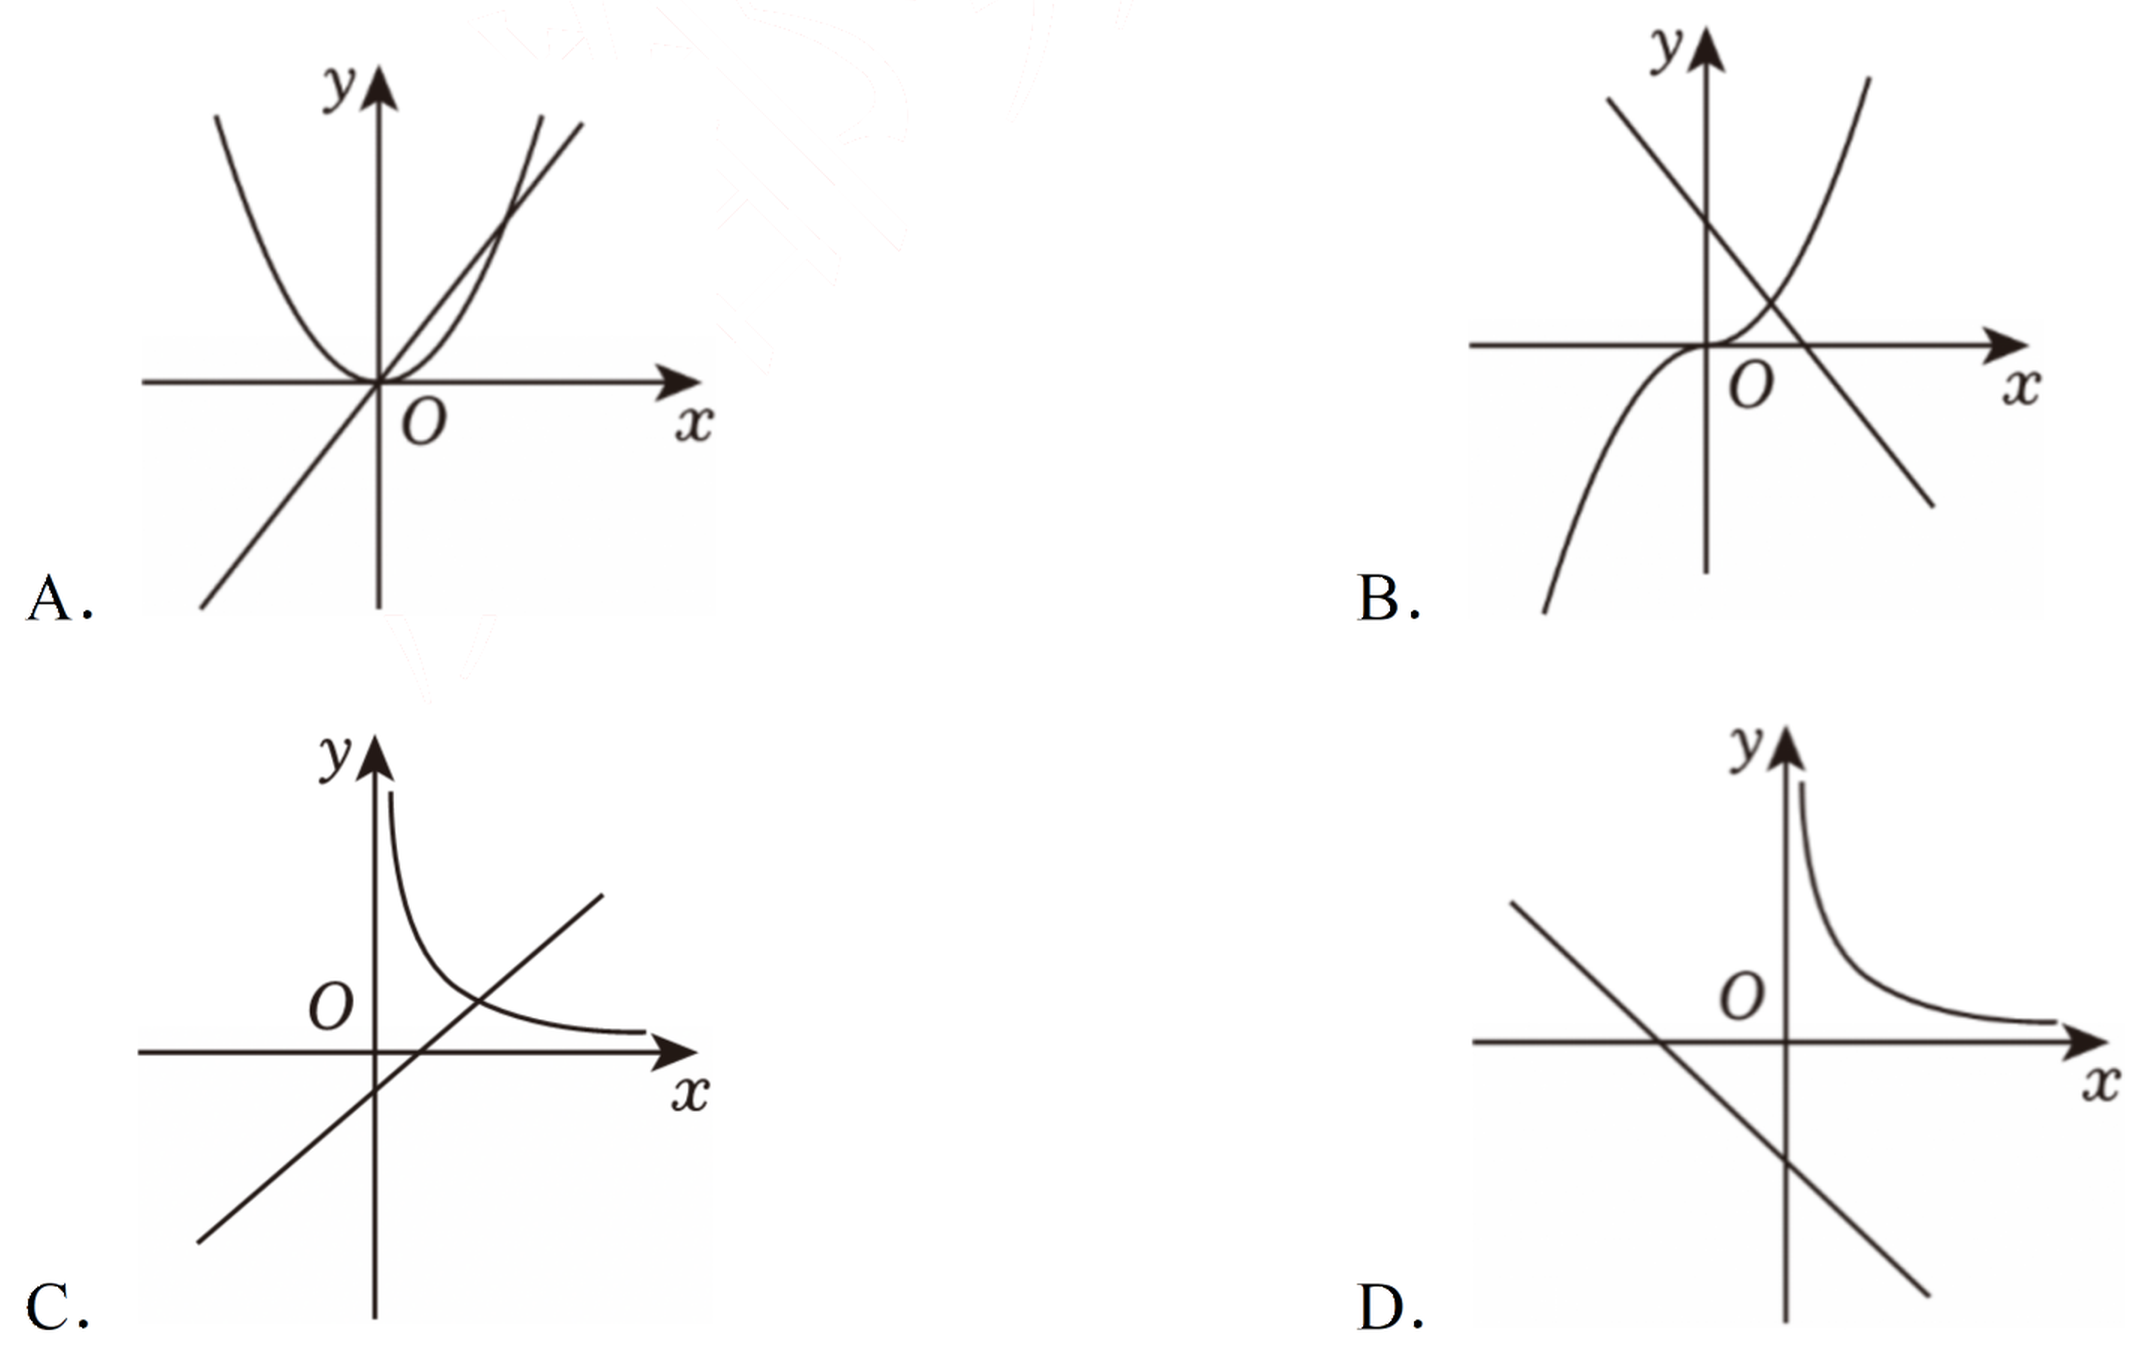
\includegraphics[width=0.80\textwidth]{figures/gao132_q14.png}
\end{center}

\ifanswer
\solbegin
\step{当 $a>0$ 时，$y=ax-\dfrac1a$ 严格增，当 $a<0$ 时，$y=ax-\dfrac1a$ 严格减，}
\step{对于 $A$，因为 $a\ne0$，所以直线 $y=ax-\dfrac1a$ 不过原点，故 $A$ 错误；}
\step{对于 $B$，由函数 $y=x^a(a\ne0)$ 的图象得 $a>1$，}
\step{由 $y=ax-\dfrac1a$ 的图象得 $a<0$，互相矛盾，故 $B$ 错误；}
\step{对于 $C$，由函数 $y=x^a(a\ne0)$ 的图象得 $a>1$，}
\step{由 $y=ax-\dfrac1a$ 的图象得 $a>0$ 且 $-\dfrac1a<0$，符合题意，故 $C$ 正确；}
\step{对于 $D$，由函数 $y=x^a(a\ne0)$ 的图象得 $a<0$，}
\step{由 $y=ax-\dfrac1a$ 的图象得 $a<0$ 且 $-\dfrac1a<0$，互相矛盾，故 $D$ 错误；}
\step{故选 $C$.}
\solend
\fi

\item 中国的 $5G$ 技术领先世界，在 $5G$ 技术中，最大数据传输速率 $C$ 取决于信道带宽 $W$，$C$ 与 $W$ 满足 $C=W\log_2\left(1+\dfrac SN\right)$，其中 $\dfrac SN$ 称为信噪比（单位：$dB$）. 若不改变带宽 $W$，初始信噪比 $\dfrac SN$ 为 $1000$，那么为了使 $C$ 增加 $30\%$，需要将信噪比 $\dfrac SN$ 从 $1000$ 提升至大约\mbox{（\quad）}

\keepwithprev
A. $5000$\qquad\qquad B. $6000$\qquad\qquad C. $7000$\qquad\qquad D. $8000$

\ifanswer
\solbegin
\step{由题意得 $\dfrac SN=1000$ 时，$C=W\log_2(1+1000)\approx W\log_2 1000$，}
\step{要使 $C$ 增加 $30\%$，则 $(1+30\%)C=W\log_2\left(1+\dfrac SN\right)$，即 $1.3C\approx W\log_2\dfrac SN$，}
\step{所以 $1.3\approx\log_{1000}\dfrac SN=\dfrac{\lg\frac SN}{\lg1000}$，所以 $\lg\dfrac SN=3.9$，所以 $\dfrac SN=10^{3.9}\approx8000$.}
\step{故选 $D$.}
\solend
\fi

\item 对于 $a\in\R$，设非空集合 $A=\left\{x\mid\dfrac{(x^2-930x+a)(x-52)}{x+a}=0\right\}$，记 $A$ 中的所有元素之和为 $S(a)$，所有元素之积为 $T(a)$，则下列说法中，不正确的是\mbox{（\quad）}

\keepwithprev
A. 存在实数 $a$，使得 $S(a)=930$

B. 存在实数 $a$，使得 $T(a)=517$

C. 不存在实数 $a$，使得 $T(a)=0$

D. 恰存在 $1$ 个实数 $a$，使得 $T(a)=-52$

\ifanswer
\solbegin
\step{由分式值为 $0$，得分子为 $0$ 且分母不为 $0$，}
\step{分子 $(x^2-930x+a)(x-52)=0$ 的根为 $x=52$}
\step{及方程 $x^2-930x+a=0$ 的两根 $x_1$，$x_2$，}
\step{由根与系数的关系得 $x_1+x_2=930$，$x_1\cdot x_2=a$，}
\step{分母限制 $x\ne-a$，需要剔除等于 $-a$ 的根，}
\step{选项 $A$，取 $a=-52$，$x=52$ 为增根舍去，集合 $A=\{x_1,x_2\}$，}
\step{元素之和 $S(a)=930$，故 $A$ 正确；}
\step{选项 $B$，当无增根时，$T(a)=52a$，令 $52a=517$，得 $a=\dfrac{517}{52}$，}
\step{验证无增根，存在这样的 $a$，故 $B$ 正确；}
\step{选项 $C$，若 $T(a)=0$，则 $0\in A$，代入分子得 $a=0$，}
\step{但 $a=0$ 时分母 $x\ne0$，$x=0$ 为增根，$0$ 不能属于集合 $A$，}
\step{故不存在 $a$ 使得 $T(a)=0$，故 $C$ 正确；}
\step{选项 $D$，当无增根时，令 $52a=-52$，得 $a=-1$；}
\step{当 $x=-a$ 是二次方程的根且不等于 $52$ 时，}
\step{令 $52\times(930+a)=-52$，解得 $a=-931$，验证符合条件；}
\step{当 $a=-52$ 时，$x=52$，舍去，}
\step{集合 $A=\{x_1,x_2\}$，$T(a)=a=-52$，得到两个满足条件的 $a$；}
\step{因此存在 $3$ 个满足条件的 $a$，故 $D$ 错误.}
\step{故选 $D$.}
\solend
\fi

\end{enumerate}

\bigsec{三、解答题}

\begin{enumerate}
\setcounter{enumi}{16}

\item 已知全集 $U=\R$，集合 $A=\left\{x\mid\dfrac{x}{x-3}<0\right\}$，$B=\{x\mid(x-a)(x+4-a)<0\}$.

(1) 当 $a=2$ 时，求 $\overline{B}$、$A\cap\overline{B}$；

(2) 若 $A\cap B=A$，求实数 $a$ 的取值范围.

\ifanswer
\solbegin
\step{(1) $\dfrac{x}{x-3}<0$，即 $x(x-3)<0$，解得 $A=\{x\mid0<x<3\}$，}
\step{当 $a=2$ 时，$B=\{x\mid(x-a)(x+4-a)<0\}=\{x\mid-2<x<2\}$，}
\step{则 $\overline{B}=\{x\mid x\leq-2$ 或 $x\geq2\}$，故 $A\cap\overline{B}=\{x\mid2\leq x<3\}$；}
\step{(2) $A\cap B=A$，则 $A\subseteq B$，故 $\begin{cases}a-4\leq0\\a\geq3\end{cases}$，解得 $3\leq a\leq4$，}
\step{故实数 $a$ 的取值范围是 $\{a\mid3\leq a\leq4\}$.}
\solend
\fi

% 第 18 题是"题干 + 图"约 7cm 的一整块，守卫放在 \item 之前
\needvspace{7cm}
\item 如图，$OA$、$OB$ 是两条长度足够长的互相垂直的笔直小路，矩形 $OCPD$ 的顶点 $C$、$D$ 分别在 $OA$、$OB$ 上，且该矩形区域内种满了荷花. 为了让观赏者有更好的观赏体验，现计划经过点 $P$ 修一条小路 $EF$，其中点 $E$ 在小路 $OA$ 上，点 $F$ 在小路 $OB$ 上，并在 $\triangle OEF$ 区域内种满荷花. 已知 $OD=25m$，$OC=40m$，且小路 $EF$ 要完全位于一个以 $O$ 为顶点的，边长为 $100$ m 的正方形内部（包括边界）. 记 $\triangle OEF$ 的面积为 $S$m$^2$.

(1) 设 $EC=x\cdot m$，试用 $x$ 表示 $OF$，并求 $x$ 的取值范围.

(2) 当 $EC$ 的长度为多少时，$S$ 取得最小值？最小值是多少？

\begin{center}
% 图取原卷 07 页截图去粉色水印，3× LANCZOS 放大
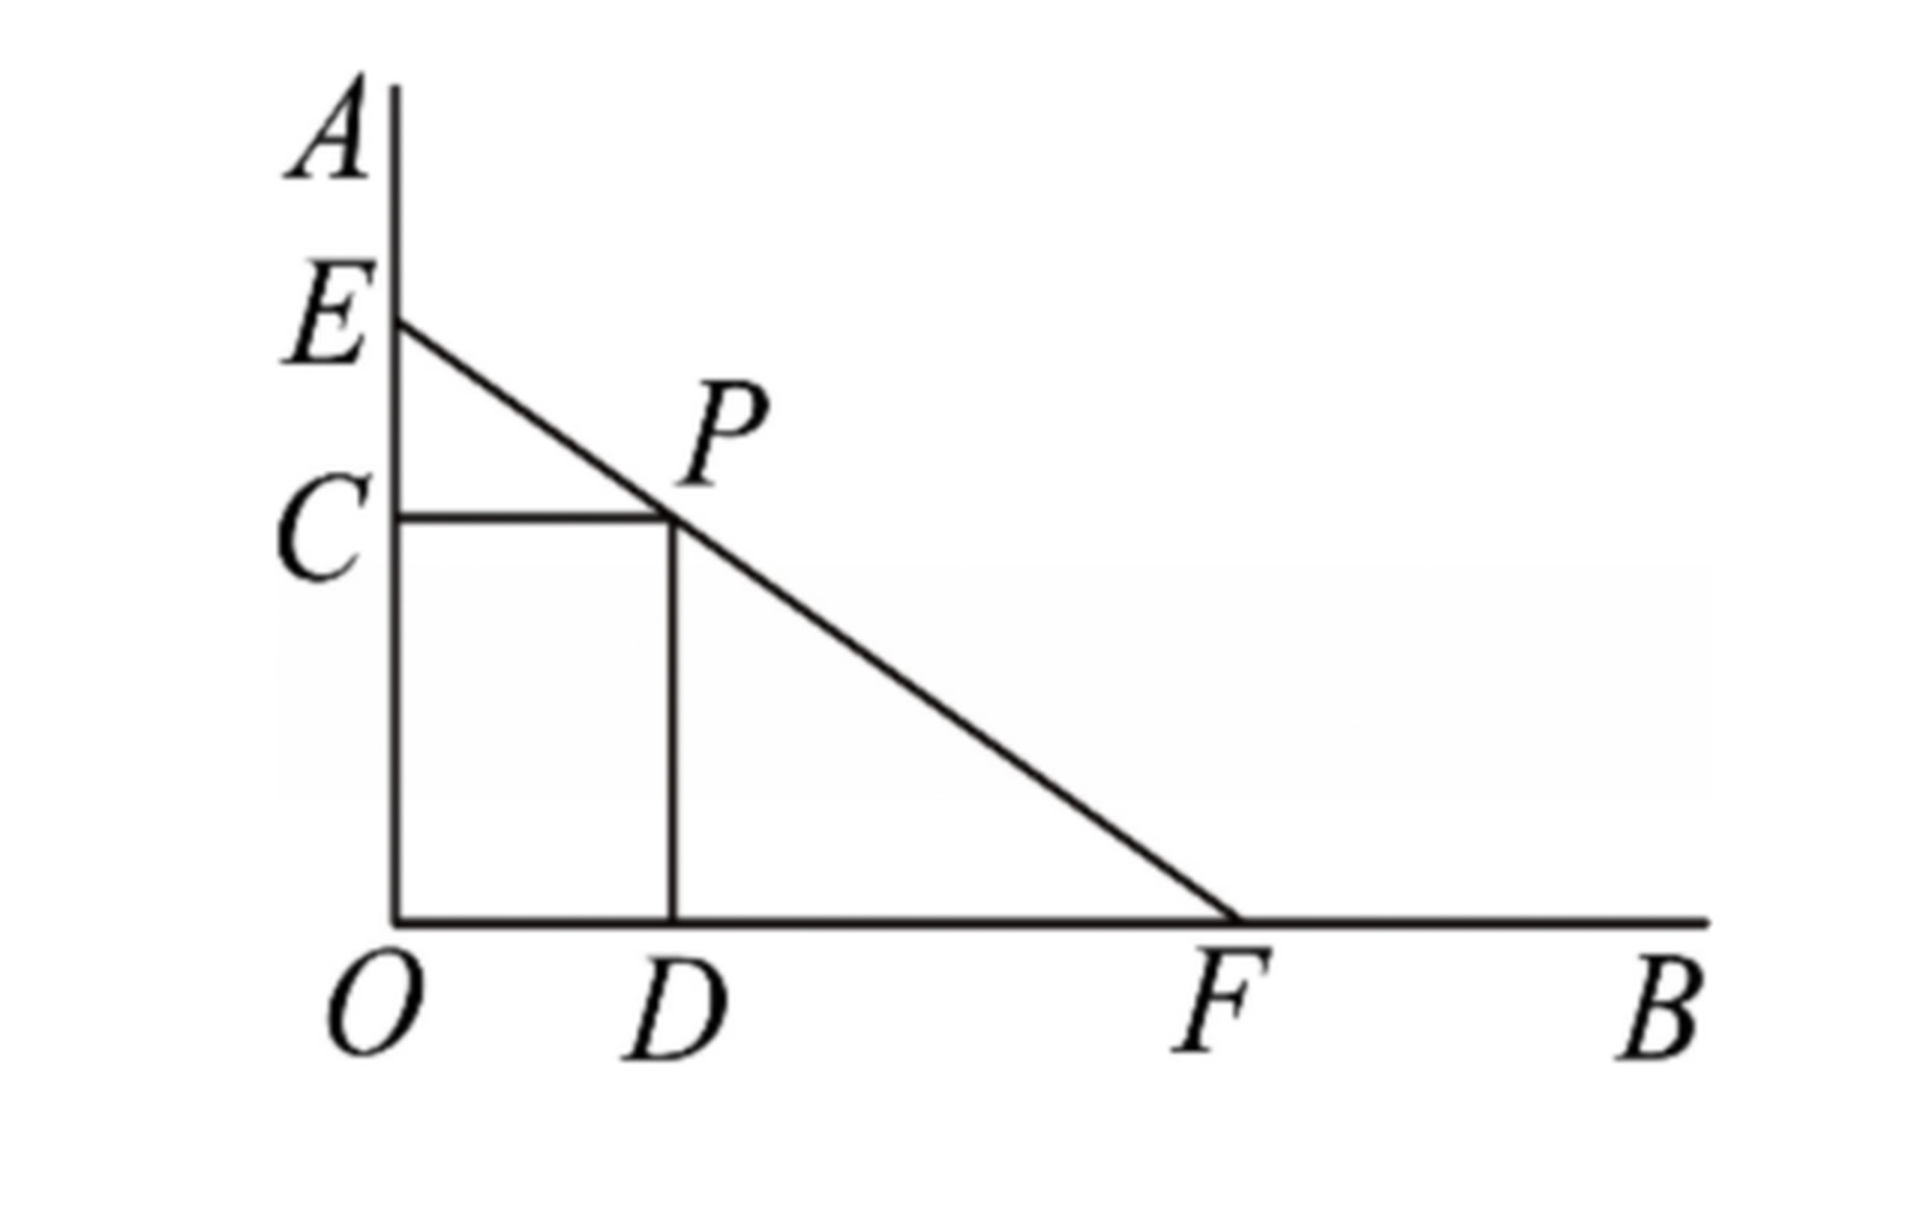
\includegraphics[width=0.32\textwidth]{figures/gao132_q18.png}
\end{center}

\ifanswer
\solbegin
\step{(1) 由题意得 $x\leq60$，}
\step{$\triangle PCE\sim\triangle FDP$，所以 $\dfrac{EC}{CP}=\dfrac{PD}{DF}$，即 $\dfrac{x}{25}=\dfrac{40}{DF}$，得 $DF=\dfrac{1000}{x}$m，}
\step{所以 $OF=OD+DF=\left(25+\dfrac{1000}x\right)$m，}
\step{所以 $25+\dfrac{1000}x\leq100$，解得 $x\geq\dfrac{40}3$；}
\step{综上，$\dfrac{40}3\leq x\leq60$；}
\step{(2) 由 $OE=OC+CE=(40+x)$m，}
\step{所以 $S=\dfrac12 OF\cdot OE=\dfrac12\left(25+\dfrac{1000}x\right)(40+x)$}
\step{$=\dfrac12\left(1000+25x+\dfrac{40000}x+1000\right)$m$^2$，}
\step{由基本不等式得 $S\geq\dfrac12\left(2000+2\sqrt{25x\cdot\dfrac{40000}x}\right)=2000$m$^2$，}
\step{当且仅当 $25x=\dfrac{40000}x$，即 $x=40$ 时取等号，}
\step{故 $EC=40$m 时，$S$ 取得最小值，为 $2000$m$^2$.}
\solend
\fi

\item 已知 $a>0$，$b>0$，请选择适当的方法证明.

(1) 若 $a\ne b$，证明：$a^3+b^3>a^2b+ab^2$；

(2) 若 $ab=1$，证明：$a^2+a<2$ 与 $b^2+b<2$ 不能同时成立.

\ifanswer
\solbegin
\step{(1) 因为 $a>0$，$b>0$，$a\ne b$，}
\step{所以 $a^3+b^3-a^2b-ab^2=a^2(a-b)+b^2(b-a)$}
\step{$=(a^2-b^2)(a-b)=(a-b)^2(a+b)>0$，所以 $a^3+b^3>a^2b+ab^2$.}
\step{(2) 假设 $a^2+a<2$ 与 $b^2+b<2$ 同时成立，所以 $-2<a<1,-2<b<1$，}
\step{又因为 $a>0,b>0$，所以 $0<a<1,0<b<1$，}
\step{所以 $0<ab<1$，这与 $ab=1$ 矛盾，}
\step{故 $a^2+a<2$ 与 $b^2+b<2$ 不可能同时成立.}
\solend
\fi

\item 若设 $M(a,n)=\lvert ax-1\rvert+\lvert ax-2\rvert+\cdots+\lvert ax-n\rvert$ 为曼哈顿扩张距离，它由 $n$ 个绝对值之和组成，其中 $n$ 为正整数.

(1) 若 $M(2,1)\leq5$，求 $x$ 的取值范围；

(2) 若 $k\leq M(2,2)$ 对一切实数 $x$ 恒成立，求实数 $k$ 的取值范围；

(3) $M(2,6)$ 是否存在最小值？若存在，求出该最小值与此时实数 $x$ 的取值范围；若不存在，说明理由.

\ifanswer
\solbegin
\step{(1) $M(2,1)=\lvert2x-1\rvert\leq5$，则不等式可化为 $-5\leq2x-1\leq5$，解得 $-2\leq x\leq3$，}
\step{所以 $x$ 的取值范围为 $[-2,3]$.}
\step{(2) 因为 $k\leq M(2,2)=\lvert2x-1\rvert+\lvert2x-2\rvert$ 对一切实数 $x$ 恒成立，}
\step{又 $\lvert2x-1\rvert+\lvert2x-2\rvert\geq\lvert(2x-1)-(2x-2)\rvert=1$，}
\step{当且仅当 $(2x-1)(2x-2)\leq0$，即 $\dfrac12\leq x\leq1$ 时取等号，}
\step{故 $k\leq1$，所以实数 $k$ 的取值范围为 $(-\infty,1]$.}
\step{(3) $M(2,6)=\lvert2x-1\rvert+\lvert2x-2\rvert+\lvert2x-3\rvert+\lvert2x-4\rvert+\lvert2x-5\rvert+\lvert2x-6\rvert$}
\step{$=2\left(\left\lvert x-\dfrac12\right\rvert+\lvert x-1\rvert+\left\lvert x-\dfrac32\right\rvert+\lvert x-2\rvert+\left\lvert x-\dfrac52\right\rvert+\lvert x-3\rvert\right)$，}
\step{其中 $\left\lvert x-\dfrac12\right\rvert+\lvert x-1\rvert+\left\lvert x-\dfrac32\right\rvert+\lvert x-2\rvert+\left\lvert x-\dfrac52\right\rvert+\lvert x-3\rvert$ 的几何意义为}
\step{在数轴上一点 $x$ 到 $\dfrac12,1,\dfrac32,2,\dfrac52,3$ 的距离之和，}
\step{要想距离之和最小，其中 $x\in\left[\dfrac12,3\right]$ 时，$\left\lvert x-\dfrac12\right\rvert+\lvert x-3\rvert$ 取得最小值，}
\step{当 $x\in\left[1,\dfrac52\right]$ 时，$\lvert x-1\rvert+\left\lvert x-\dfrac52\right\rvert$ 取得最小值，}
\step{当 $x\in\left[\dfrac32,2\right]$ 时，$\left\lvert x-\dfrac32\right\rvert+\lvert x-2\rvert$ 取得最小值，}
\step{综上，当 $x\in\left[\dfrac32,2\right]$ 时，$\left\lvert x-\dfrac12\right\rvert+\lvert x-1\rvert+\left\lvert x-\dfrac32\right\rvert+\lvert x-2\rvert+\left\lvert x-\dfrac52\right\rvert+\lvert x-3\rvert$}
\step{取得最小值，最小值为 $3-\dfrac12+\dfrac52-1+2-\dfrac32=\dfrac92$，}
\step{故 $M(2,6)=2\left(\left\lvert x-\dfrac12\right\rvert+\lvert x-1\rvert+\left\lvert x-\dfrac32\right\rvert+\lvert x-2\rvert+\left\lvert x-\dfrac52\right\rvert+\lvert x-3\rvert\right)$ 的}
\step{最小值为 $9$.}
\solend
\fi

\item 已知集合 $A=\{a_1,a_2,\cdots,a_n\}(0\leq a_1<a_2<\cdots<a_n,n\in\N,n\geq3)$ 具有性质 $Q$：对任意 $i,j(1\leq i\leq j\leq n)$，$a_i+a_j$ 与 $a_j-a_i$ 至少有一个属于集合 $A$；

(1) 判断集合 $M=\{0,2,4\}$ 与 $N=\{2,3,4\}$ 是否具有性质 $Q$，并说明理由；

(2) 已知 $A=\{a_1,a_2,a_3\}$ 具有性质 $Q$，当 $a_2=2026$ 时，求集合 $A$；

(3) 已知 $B=\{b_1,b_2,\cdots,b_{2026}\}$ 具有性质 $Q$，求 $\dfrac{b_1+b_2+\cdots+b_{2026}}{b_{2026}}$ 的值；

\ifanswer
\solbegin
\step{(1) 集合 $M=\{0,2,4\}$ 中，}
\step{因为 $0+2\in M,0+4\in M,4-2\in M,0\pm0=0\in M$，}
\step{$2+2=4\in M,2-2=0\in M,4-4=0\in M$，所以集合 $M$ 具有性质 $Q$；}
\step{集合 $N=\{2,3,4\}$ 中，因为 $3+3=6\notin N,3-3=0\notin N$，}
\step{所以集合 $N$ 不具有性质 $Q$.}
\step{(2) 因为 $a_1<a_2<a_3$，且 $A=\{a_1,a_2,a_3\}$ 具有性质 $Q$，}
\step{所以 $a_3+a_3\notin A,a_3-a_3=0\in A$，则 $a_1=0$，}
\step{又因为 $a_2+a_3>a_3$，所以 $a_2+a_3\notin A$，则 $a_3-a_2\in A$，}
\step{由集合的互异性得 $a_3-a_2=a_2$，而 $a_2=2026$，所以 $a_3=4052$，}
\step{故 $A=\{0,2026,4052\}$；}
\step{(3) 先证明一般结论：$A=\{a_1,a_2,\cdots,a_n\}(0\leq a_1<a_2<\cdots<a_n,n\in\N,n\geq3)$}
\step{具有性质 $Q$，则 $a_1+a_2+a_3+\cdots+a_n=\dfrac n2 a_n$.}
\step{因为 $A=\{a_1,a_2,\cdots,a_n\}(0\leq a_1<a_2<\cdots<a_n,n\in\N,n\geq3)$ 具有性质 $Q$，}
\step{所以 $a_n+a_n\notin A$，则 $a_n-a_n=0\in A$，则 $a_1=0$.}
\step{又因为 $0\leq a_1<a_2<\cdots<a_n$，所以 $0\leq a_n-a_n<a_n-a_{n-1}<\cdots<a_n-a_1$，}
\step{又因为 $a_n+a_{n-i}>a_n(i=1,2,\cdots,n-1)$，所以 $a_n+a_{n-i}\notin A$，}
\step{则 $a_n-a_{n-i}\in A$，}
\step{所以 $a_1=a_n-a_n,a_2=a_n-a_{n-1},a_3=a_n-a_{n-2},\cdots,a_n=a_n-a_1$.}
\step{所以 $a_1+a_2+a_3+\cdots+a_n$}
\step{$=(a_n-a_n)+(a_n-a_{n-1})+(a_n-a_{n-2})+\cdots+(a_n-a_1)$，}
\step{即 $a_1+a_2+a_3+\cdots+a_n=\dfrac n2 a_n$，}
\step{所以 $B=\{b_1,b_2,\cdots,b_{2026}\}$ 具有性质 $Q$，则 $b_1+b_2+\cdots+b_{2026}=\dfrac{2026}{2}b_{2026}$，}
\step{所以 $\dfrac{b_1+b_2+\cdots+b_{2026}}{b_{2026}}=\dfrac{2026}{2}=1013$.}
\solend
\fi

\end{enumerate}

% 行数复核：逐题数 \step 条数，合计 144 条（Q3：4；Q4：1；Q5：4；Q6：2；Q7：9；Q8：2；
% Q9：3；Q10：6；Q11：9；Q12：9；Q13：0；Q14：9；Q15：4；Q16：19；Q17：5；Q18：11；
% Q19：7；Q20：17；Q21：23），与原卷印刷行逐题相等（cases 块作一个印刷行计）。
% 第 13 题只印括号内答案、提 \ans{}，不计入 \step 账；第 14—16 题答案在解析末句，
% 括号内留空、不另提 \ans{}。

\end{document}
"
% 紧凑版：xelatex "\def\iscompact{1}% 高一132_川沙中学_期中.tex
%   —— 高一上数学"2026-2027 年川沙中学高一上期中"（试卷版/答案版）
% 试卷版：xelatex 高一132_川沙中学_期中.tex
% 答案版：xelatex "\def\isanswer{1}\input{高一132_川沙中学_期中.tex}"
% 紧凑版：xelatex "\def\iscompact{1}\input{高一132_川沙中学_期中.tex}"
%
% 原始材料：微信公众号"魔都数学加油站"文章，作者破晓，2026-11-14 19:00 发布；
% 连载"27学年高一132"，原文标题"27学年高一132——2026-2027年上海市川沙中学高一上期中"；
% 原文链接：https://mp.weixin.qq.com/s/VBG01CrUNMIYWWHhSfz8JQ。
% 正文为 11 张 PNG 页（01、04、06、07、09、11 为 2560x3620，02、03、05、08、10 为 4762x6735），
% 题目下印有【解析】，为讲评版。题目、解析均据原图转录；
% 卷面粉红色水印"魔都数学加油站"及公众号页脚未录入。全卷 2 幅插图：第 14 题四幅坐标图选项、
% 第 18 题矩形 OCPD 与小路 EF 示意图，均取原卷 04／07 页截图去水印。
%
% 卷首标题：原卷印作"2026-2027 年川沙中学高一上期中"（公众号标题中的"上海市"
% 卷面标题行没有，本稿照卷面），年份区间按全稿惯例排 en dash；原卷未印副标题，
% 本卷为期中卷、跨集合与常用逻辑用语／不等式／函数三章，按题目内容标为
% "集合与常用逻辑用语、不等式、函数"（与 125／126／128／129／131 同期中卷口径相同）：
% 集合与逻辑见 Q5、Q6、Q17、Q21，不等式见 Q3、Q4、Q9、Q10、Q12、Q13、Q15、Q16、Q19，
% 函数（幂函数、指数／对数、基本不等式应用）见 Q7、Q8、Q11、Q14、Q18、Q20。
%
% 题号体例：本卷共 19 题——一、填空题 3—12（10 题）、二、选择题 13—16（4 题）、
% 三、解答题 17—21（5 题）。三节分别 \setcounter{enumi}{2}／{12}／{16}。
%
% 与原卷的排版差异：
%   ① 原文从第 3 题起，本稿保留原题号（见上"题号体例"）；
%   ② 原卷每题下直接印【解析】，本稿按全稿惯例置于答案版；第 13 题答案 D 印在题干
%      括号内、无独立答案段，按 高一37／52／53／55／63／64／128／131 成例括号留空、
%      另提 \ans{$D$}；第 14—16 题答案在解析末句"故选 …"，括号内留空、不另提 \ans{}；
%   ③ 原卷未印副标题，本稿按"知识模块"口径补出；
%   ④ 原卷填空横线按全稿惯例排为 \blankline[4.4em]；选择题括号排 \mbox{（\quad）}、
%      选项段前按惯例加 \keepwithprev；解答题不留作答区（原卷为讲评版，与 109—131 同）；
%   ⑤ 原卷数集排斜体 $R^+$／$R$／$Z$／$N$，按全稿惯例改 \R^+／\R／\Z／\N；
%      绝对值排 \lvert…\rvert，集合描述竖线排 \mid；不等号按全稿惯例排 \leqslant／\geqslant；
%      补集照原卷上划线排 \overline{B}；
%   ⑥ 子题标号 (1)(2)(3) 原卷用半角括号，照录；第 14 题四幅坐标图选项按原卷 2×2 排布
%      合并裁为一张 \includegraphics（未用 TikZ 重绘，以保证与原卷一致），题前加
%      \needvspace{9cm} 守卫；第 18 题图取 07 页截图，题前按惯例加 \needvspace{7cm} 守卫
%      （照 高一120／127／129／131 成例），两者守卫都放在 \item 之前；
%   ⑦ 原卷 Q7 解析跨 01—02 页、Q10 解析跨 02—03 页、Q12 解析跨 03—04 页、
%      Q14 解析跨 04—05 页、Q16 解析在 06 页、Q18 解析跨 07—08 页、
%      Q20 解析跨 08—09 页、Q21 解析跨 10—11 页，本稿按题合并连续排版；
%      末页第 11 页为 Q21 (3) 解析的续尾，按实际印刷行单列。
%
% 判别式字形：第 10 题 $\triangle=4(a-1)^2+16(a-1)<0$、第 11 题
%   $\triangle=4(m-2)^2-4(m^2-3m+3)=-4m+4>0$ 两处原卷均排 $\triangle$（等边、扁），
%   逐处放大核对、字形一致，照录 \triangle；与 高一129／131 同题排 $\Delta$（等腰、高）不同。
%   全卷 \triangle 兼作第 18 题「$\triangle PCE\sim\triangle FDP$」「$\triangle OEF$」的几何
%   三角形记号，全卷未出现 \Delta。
%
% 子集符号：第 5 题解析 $B\subseteq A$、第 17 题 (2) 解析 $A\subseteq B$ 均印带下划线，
%   照录 \subseteq；全卷未出现单线 \subset。
%
% 原卷存疑照录：
%   第 9 题题干作"充分非必要条件"、解析作"充分不必要条件"，措辞不同，照录；
%   第 10 题解析"当 $a-1=0$ 时，$-4\geq0$，不等式不成立，$a=1$ 满足题意"照录；
%   第 11 题解析"所以 $2(m-1)+\dfrac1{m-1}\leq-2\sqrt2$"由上一行 $2(1-m)+\dfrac1{1-m}\geq2\sqrt2$
%     直接变号得到，照录；
%   第 12 题解析"由 $x\in Z$，$-7<-2\sqrt{10}<-6$"与"即 $k^2+7k+10\leq0$，解得 $-5\leq k\leq-2$"照录；
%   第 16 题解析"令 $52\times(930+a)=-52$，解得 $a=-931$"（按式应为 $a=-931$ 之外的解）照录；
%   第 19 题 (2) 解析"所以 $-2<a<1,-2<b<1$"数学式内半角逗号，照录；
%   第 20 题 (3) 解析"最小值为 $3-\dfrac12+\dfrac52-1+2-\dfrac32=\dfrac92$"与
%     "故 $M(2,6)=\dots$ 的最小值为 9"两处结论并列，照录；
%   第 21 题 (1) 解析"$0+2\in M,0+4\in M,4-2\in M,0\pm0=0\in M$"、
%     "$2+2=4\in M,2-2=0\in M,4-4=0\in M$"、(3) 各连写等式内半角逗号，照录；
%   第 21 题 (3) 解析"即 $a_1+a_2+a_3+\cdots+a_n=\dfrac n2 a_n$，"句末用半角逗号，照录。
%
% 行数复核：见文末"行数复核"注（逐题 \step 条数与原卷印刷行逐题相等，cases 块作一个印刷行计）。
%   第 13 题只印括号内答案、提 \ans{}，不计入 \step 账；第 14—16 题答案在解析末句，
%   括号内留空、不另提 \ans{}。
%
\documentclass[a4paper,11pt]{article}
\usepackage{common}

\begin{document}

\examtitlest[3]{2026--2027 年川沙中学高一上期中}{集合与常用逻辑用语、不等式、函数}

\bigsec{一、填空题}

\begin{enumerate}
\setcounter{enumi}{2}

\item 已知 $a$、$b\in\R^+$ 且 $ab=2$，则 $a+2b$ 的最小值为\blankline[4.4em].

\ifanswer
\solbegin
\step{因为 $a\in\R^+$，$b\in\R^+$ 且 $ab=2$，}
\step{由基本不等式得 $a+2b\geq2\sqrt{a\cdot2b}=2\sqrt{2ab}=2\sqrt4=4$.}
\step{等号当且仅当 $a=2b$ 时成立，结合 $ab=2$ 解得 $b=1$，$a=2$，}
\step{所以 $a+2b$ 的最小值为 $4$.}
\solend
\fi

\item 如果幂函数 $f(x)=(m^2-3m-3)x^{m^2+m-3}$ 在 $(0,+\infty)$ 上是增函数，则实数 $m=$\blankline[4.4em].

\ifanswer
\solbegin
\step{由已知得 $\begin{cases}m^2-3m-3=1\\m^2+m-3>0\end{cases}$，所以 $m=4$.}
\solend
\fi

\item 已知集合 $A=\{1,2\}$，集合 $B=\{x\mid ax=6\}$，若 $A\cup B=A$，则 $a$ 的所有取值构成的集合为\blankline[4.4em].

\ifanswer
\solbegin
\step{因为 $A\cup B=A$，所以 $B\subseteq A$，}
\step{当 $a=0$ 时，$B=\varnothing$，满足 $B\subseteq A$；}
\step{当 $a\ne0$ 时，$B=\left\{\dfrac6a\right\}$，则 $\dfrac6a=1$ 或 $\dfrac6a=2$，解得 $a=6$ 或 $a=3$，}
\step{综上所述，$a$ 的所有取值构成的集合为 $\{0,3,6\}$.}
\solend
\fi

\item 设全集为 $\R$，$A=\{y\mid y=-x^2+2x+1\}$，$B=\{x\mid y=\ln(x-1)\}$，则 $A\cap B=$\blankline[4.4em].

\ifanswer
\solbegin
\step{$A=\{y\mid y=-x^2+2x+1\}=\{y\mid y=-(x-1)^2+2\}=\{y\mid y\leq2\}$，}
\step{$B=\{x\mid y=\ln(x-1)\}=\{x\mid x>1\}$，则 $A\cap B=(1,2]$.}
\solend
\fi

\item 已知 $x\in\R$，则方程 $\lvert 6-x\rvert+\lvert 6x-3\rvert=\lvert 5x+3\rvert$ 的解集为\blankline[4.4em].

\ifanswer
\solbegin
\step{当 $x<-\dfrac35$ 时，$6-x>0$，$6x-3<0$，$5x+3<0$，}
\step{原方程为 $6-x-6x+3=-5x-3$，解得 $x=6$，不满足 $x<-\dfrac35$；}
\step{当 $-\dfrac35\leq x\leq\dfrac12$ 时，$5x+3\geq0$，$6x-3<0$，$6-x>0$，}
\step{原方程为 $6-x+3-6x=5x+3$，解得 $x=\dfrac12$；}
\step{当 $\dfrac12<x\leq6$ 时，$5x+3>0$，$6x-3>0$，$6-x\geq0$，}
\step{原方程为 $6-x+6x-3=5x+3$，即 $0=0$，恒成立，所以 $\dfrac12<x\leq6$；}
\step{当 $x>6$ 时，$5x+3\geq0$，$6x-3>0$，$6-x<0$，}
\step{原方程为 $x-6+6x-3=5x+3$，解得 $x=6$，不满足 $x>6$；}
\step{综上 $\dfrac12\leq x\leq6$，所以原方程的解集为 $\left\{x\mid\dfrac12\leq x\leq6\right\}$.}
\solend
\fi

\item 已知 $\log_2 3=a,2^b=7$，用 $a,b$ 表示 $\log_{42}56$ 为\blankline[4.4em].

\ifanswer
\solbegin
\step{$\log_{42}56=\dfrac{\log_2 56}{\log_2 42}=\dfrac{\log_2(7\times8)}{\log_2(6\times7)}=\dfrac{\log_2 7+\log_2 8}{\log_2 6+\log_2 7}$}
\step{$=\dfrac{\log_2 7+\log_2 2^3}{\log_2 2+\log_2 3+\log_2 7}=\dfrac{b+3}{1+a+b}$.}
\solend
\fi

\item 已知 $\dfrac13<x<\dfrac12$ 是不等式 $\lvert x-m\rvert<1$ 成立的充分非必要条件，则 $m$ 的取值范围是\blankline[4.4em].

\ifanswer
\solbegin
\step{因为 $\lvert x-m\rvert<1$，所以 $-1<x-m<1$，所以 $m-1<x<m+1$，}
\step{所以 $m-1<x<m+1$ 成立的充分不必要条件是 $\dfrac13<x<\dfrac12$，}
\step{所以 $\begin{cases}m-1\leq\dfrac13\\m+1\geq\dfrac12\end{cases}$，解得 $-\dfrac12\leq m\leq\dfrac43$，故 $m$ 的取值范围是 $\left[-\dfrac12,\dfrac43\right]$.}
\solend
\fi

\item 若关于 $x$ 的不等式 $(a-1)x^2+2(a-1)x-4\geq0$ 的解集为空集，则 $a$ 的取值范围是\blankline[4.4em].

\ifanswer
\solbegin
\step{关于 $x$ 的不等式 $(a-1)x^2+2(a-1)x-4\geq0$ 的解集为 $\varnothing$，}
\step{当 $a-1=0$ 时，$-4\geq0$，不等式不成立，$a=1$ 满足题意；}
\step{当 $a-1>0$ 时，$a>1$，不等式的解集不为空集，不满足题意；}
\step{当 $a-1<0$ 时，$a<1$，当 $\triangle=4(a-1)^2+16(a-1)<0$ 时，即 $(a-1)(a+3)<0$，}
\step{解得 $-3<a<1$，满足题意；}
\step{综上，实数 $a$ 的取值范围是 $\{a\mid-3<a\leq1\}$.}
\solend
\fi

\item 已知关于 $x$ 的方程 $x^2+2(m-2)x+m^2-3m+3=0$ 有两个不相等的实数根 $x_1$、$x_2$，则 $\dfrac{mx_1}{x_1-1}+\dfrac{mx_2}{x_2-1}-\dfrac{2}{x_1+x_2-2}$ 的最大值为\blankline[4.4em].

\ifanswer
\solbegin
\step{关于 $x$ 的方程 $x^2+2(m-2)x+m^2-3m+3=0$ 有两个不相等的实数根 $x_1$、$x_2$，}
\step{则 $\triangle=4(m-2)^2-4(m^2-3m+3)=-4m+4>0$，得 $m<1$，}
\step{且 $x_1+x_2=-2(m-2)$，$x_1x_2=m^2-3m+3$，}
\step{$\dfrac{mx_1}{x_1-1}+\dfrac{mx_2}{x_2-1}-\dfrac{2}{x_1+x_2-2}=\dfrac{m[2x_1x_2-(x_1+x_2)]}{x_1x_2-(x_1+x_2)+1}+\dfrac1{m-1}$}
\step{$=\dfrac{2m(m-1)^2}{m^2-m}+\dfrac1{m-1}=2(m-1)+\dfrac1{m-1}$，}
\step{又因为 $m<1$，所以 $m-1<0$，则 $1-m>0$，}
\step{所以 $2(1-m)+\dfrac1{1-m}\geq2\sqrt{2(1-m)\cdot\dfrac1{1-m}}=2\sqrt2$，}
\step{当且仅当 $2(1-m)=\dfrac1{1-m}$ 时，即 $m=1-\dfrac{\sqrt2}2$ 时取等号，}
\step{所以 $2(m-1)+\dfrac1{m-1}\leq-2\sqrt2$，即 $\dfrac{mx_1}{x_1-1}+\dfrac{mx_2}{x_2-1}-\dfrac2{x_1+x_2-2}$ 的最大值为 $-2\sqrt2$.}
\solend
\fi

\item 若使集合 $A=\{x\mid(kx-k^2-10)(x-1)>0,x\in\Z\}$ 中的元素个数最少，则实数 $k$ 的取值范围是\blankline[4.4em].

\ifanswer
\solbegin
\step{由题意集合 $A=\{x\mid(kx-k^2-10)(x-1)>0,\ x\in\Z\}$，}
\step{$k=0$ 时，不等式解得 $x<1$，有无数个整数解；}
\step{$k\ne0$ 时，则不等式变形为 $k\left(x-k-\dfrac{10}k\right)(x-1)>0$，}
\step{当 $k>0$ 时，$k+\dfrac{10}k\geq2\sqrt{10}$，仅当 $k=\sqrt{10}$ 时等号成立，}
\step{此时不等式解得 $x>k+\dfrac{10}k$ 或 $x<1$，有无数个整数解；}
\step{当 $k<0$ 时，$k+\dfrac{10}k=-\left[(-k)+\left(-\dfrac{10}k\right)\right]\leq-2\sqrt{10}$，仅当 $k=-\sqrt{10}$ 时等号成立，}
\step{此时不等式解得 $k+\dfrac{10}k<x<1$，}
\step{由 $x\in\Z$，$-7<-2\sqrt{10}<-6$，要使集合 $A$ 中的元素最少，则 $k+\dfrac{10}k\geq-7$，}
\step{即 $k^2+7k+10\leq0$，解得 $-5\leq k\leq-2$，故实数 $k$ 的取值范围是 $[-5,-2]$.}
\solend
\fi

\end{enumerate}

\bigsec{二、选择题}

\begin{enumerate}
\setcounter{enumi}{12}

\item 下列说法正确的是\mbox{（\quad）}

\keepwithprev
A. 若 $a>b$，则 $\dfrac1a<\dfrac1b$\qquad\qquad B. 若 $a>b$，$c>d$，则 $ac>bd$

C. 若 $a>b$，则 $ac^2>bc^2$\qquad\qquad D. 若 $ac^2>bc^2$，则 $a>b$

\ifanswer
\ans{$D$}
\fi

% 第 14 题四幅坐标图选项是一整块，守卫放在 \item 之前
\needvspace{9cm}
\item 在同一坐标系内，函数 $y=x^a(a\ne0)$ 和 $y=ax-\dfrac1a$ 的图象可能是\mbox{（\quad）}

\keepwithprev
\begin{center}
% 四幅坐标图选项取原卷 04 页截图去粉色水印，按原卷 2×2 排布合并为一张
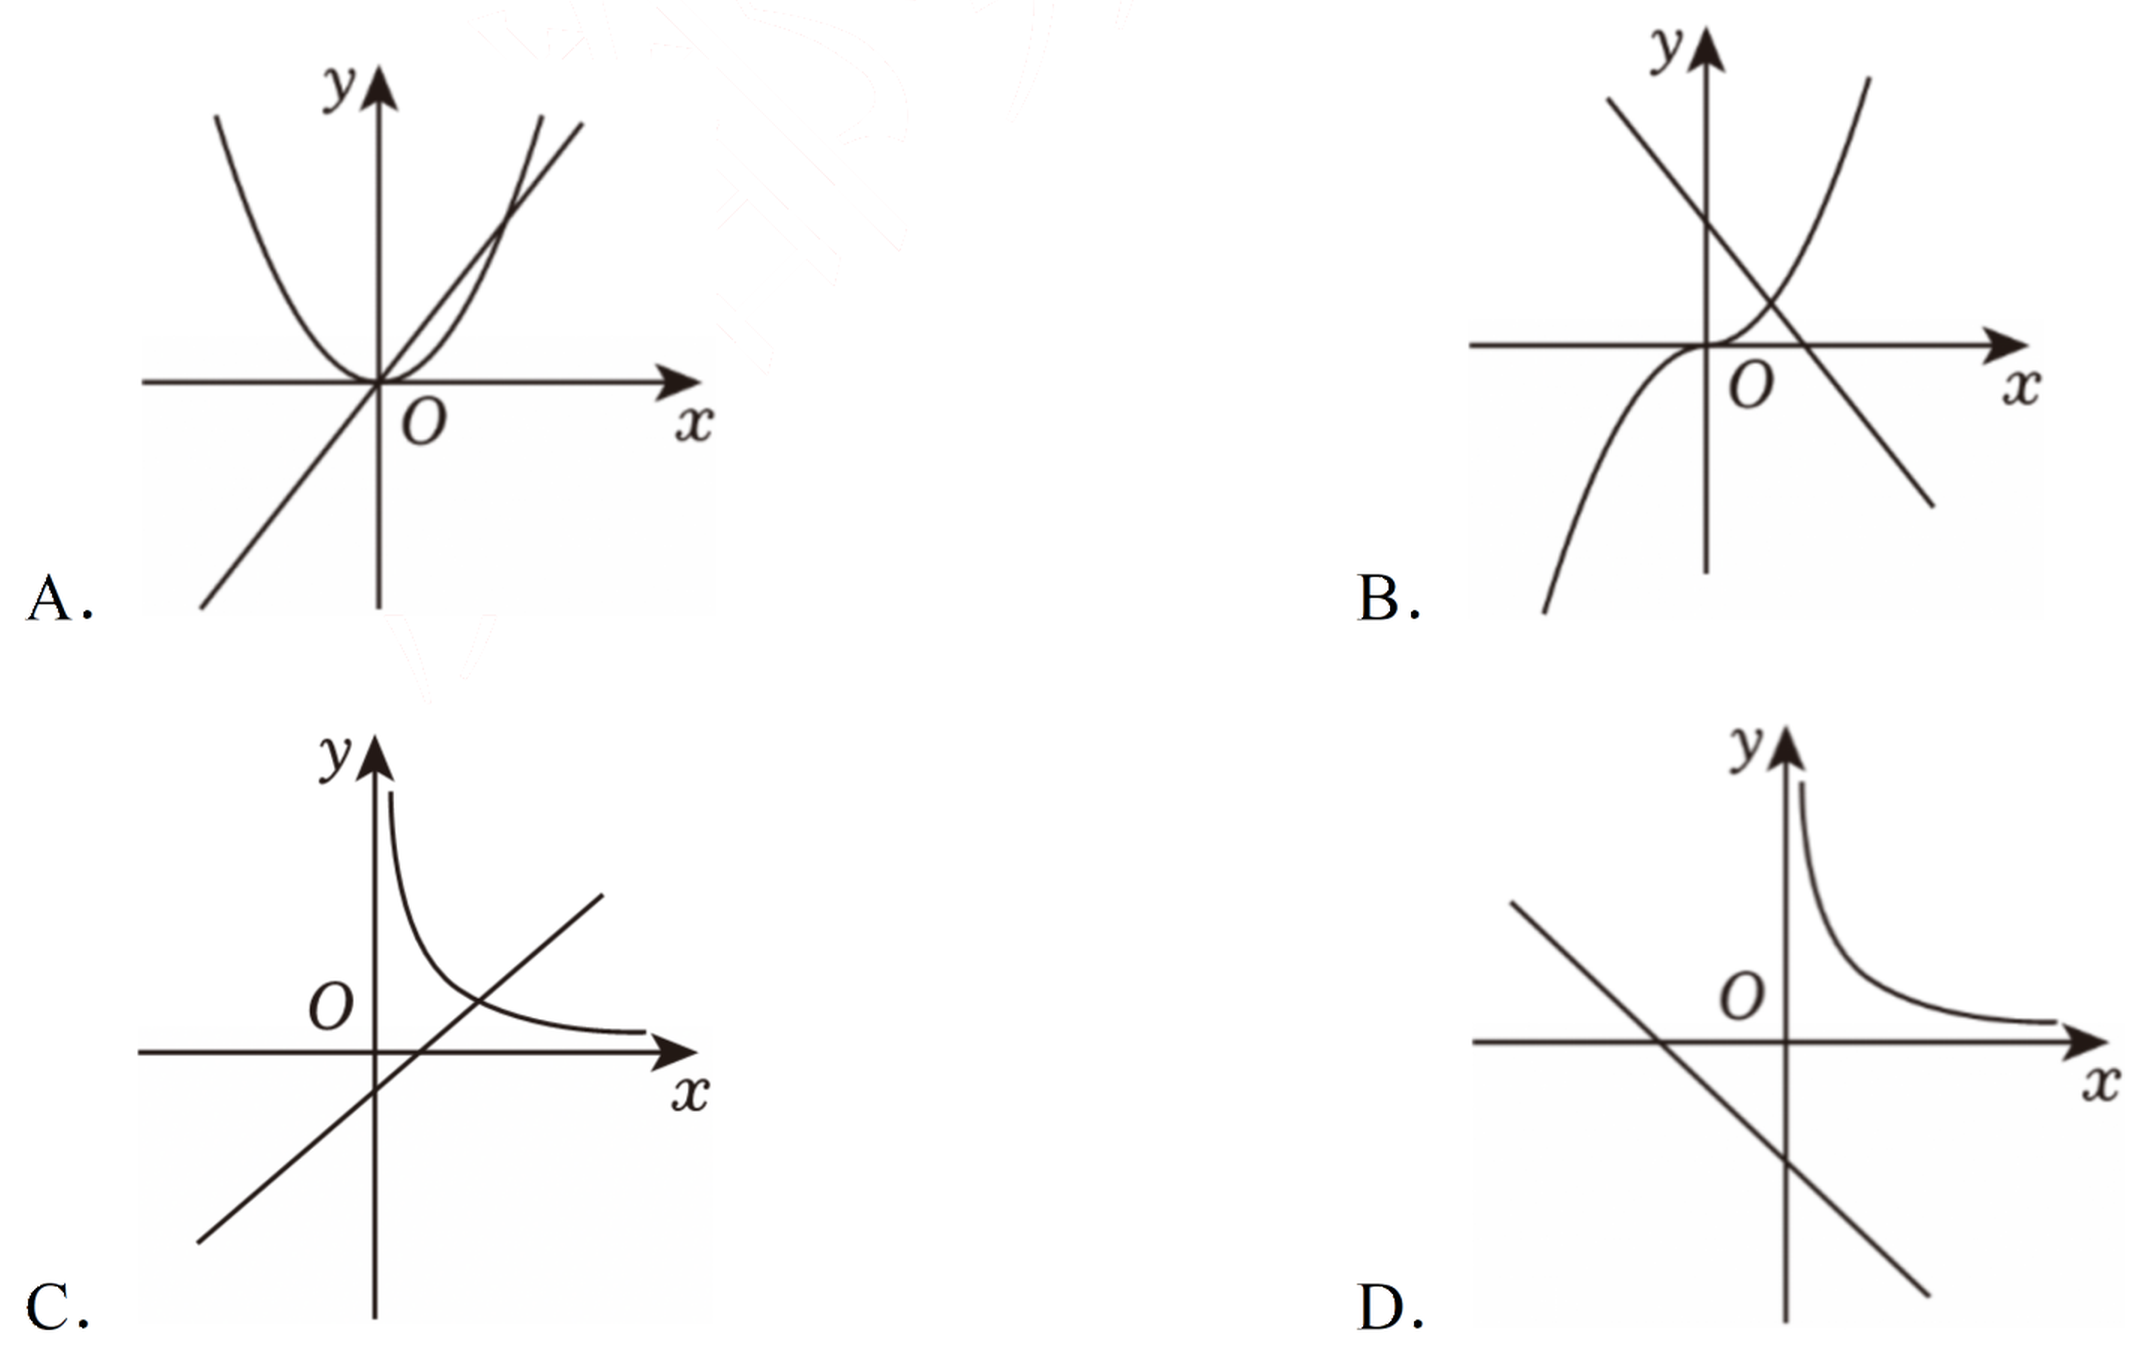
\includegraphics[width=0.80\textwidth]{figures/gao132_q14.png}
\end{center}

\ifanswer
\solbegin
\step{当 $a>0$ 时，$y=ax-\dfrac1a$ 严格增，当 $a<0$ 时，$y=ax-\dfrac1a$ 严格减，}
\step{对于 $A$，因为 $a\ne0$，所以直线 $y=ax-\dfrac1a$ 不过原点，故 $A$ 错误；}
\step{对于 $B$，由函数 $y=x^a(a\ne0)$ 的图象得 $a>1$，}
\step{由 $y=ax-\dfrac1a$ 的图象得 $a<0$，互相矛盾，故 $B$ 错误；}
\step{对于 $C$，由函数 $y=x^a(a\ne0)$ 的图象得 $a>1$，}
\step{由 $y=ax-\dfrac1a$ 的图象得 $a>0$ 且 $-\dfrac1a<0$，符合题意，故 $C$ 正确；}
\step{对于 $D$，由函数 $y=x^a(a\ne0)$ 的图象得 $a<0$，}
\step{由 $y=ax-\dfrac1a$ 的图象得 $a<0$ 且 $-\dfrac1a<0$，互相矛盾，故 $D$ 错误；}
\step{故选 $C$.}
\solend
\fi

\item 中国的 $5G$ 技术领先世界，在 $5G$ 技术中，最大数据传输速率 $C$ 取决于信道带宽 $W$，$C$ 与 $W$ 满足 $C=W\log_2\left(1+\dfrac SN\right)$，其中 $\dfrac SN$ 称为信噪比（单位：$dB$）. 若不改变带宽 $W$，初始信噪比 $\dfrac SN$ 为 $1000$，那么为了使 $C$ 增加 $30\%$，需要将信噪比 $\dfrac SN$ 从 $1000$ 提升至大约\mbox{（\quad）}

\keepwithprev
A. $5000$\qquad\qquad B. $6000$\qquad\qquad C. $7000$\qquad\qquad D. $8000$

\ifanswer
\solbegin
\step{由题意得 $\dfrac SN=1000$ 时，$C=W\log_2(1+1000)\approx W\log_2 1000$，}
\step{要使 $C$ 增加 $30\%$，则 $(1+30\%)C=W\log_2\left(1+\dfrac SN\right)$，即 $1.3C\approx W\log_2\dfrac SN$，}
\step{所以 $1.3\approx\log_{1000}\dfrac SN=\dfrac{\lg\frac SN}{\lg1000}$，所以 $\lg\dfrac SN=3.9$，所以 $\dfrac SN=10^{3.9}\approx8000$.}
\step{故选 $D$.}
\solend
\fi

\item 对于 $a\in\R$，设非空集合 $A=\left\{x\mid\dfrac{(x^2-930x+a)(x-52)}{x+a}=0\right\}$，记 $A$ 中的所有元素之和为 $S(a)$，所有元素之积为 $T(a)$，则下列说法中，不正确的是\mbox{（\quad）}

\keepwithprev
A. 存在实数 $a$，使得 $S(a)=930$

B. 存在实数 $a$，使得 $T(a)=517$

C. 不存在实数 $a$，使得 $T(a)=0$

D. 恰存在 $1$ 个实数 $a$，使得 $T(a)=-52$

\ifanswer
\solbegin
\step{由分式值为 $0$，得分子为 $0$ 且分母不为 $0$，}
\step{分子 $(x^2-930x+a)(x-52)=0$ 的根为 $x=52$}
\step{及方程 $x^2-930x+a=0$ 的两根 $x_1$，$x_2$，}
\step{由根与系数的关系得 $x_1+x_2=930$，$x_1\cdot x_2=a$，}
\step{分母限制 $x\ne-a$，需要剔除等于 $-a$ 的根，}
\step{选项 $A$，取 $a=-52$，$x=52$ 为增根舍去，集合 $A=\{x_1,x_2\}$，}
\step{元素之和 $S(a)=930$，故 $A$ 正确；}
\step{选项 $B$，当无增根时，$T(a)=52a$，令 $52a=517$，得 $a=\dfrac{517}{52}$，}
\step{验证无增根，存在这样的 $a$，故 $B$ 正确；}
\step{选项 $C$，若 $T(a)=0$，则 $0\in A$，代入分子得 $a=0$，}
\step{但 $a=0$ 时分母 $x\ne0$，$x=0$ 为增根，$0$ 不能属于集合 $A$，}
\step{故不存在 $a$ 使得 $T(a)=0$，故 $C$ 正确；}
\step{选项 $D$，当无增根时，令 $52a=-52$，得 $a=-1$；}
\step{当 $x=-a$ 是二次方程的根且不等于 $52$ 时，}
\step{令 $52\times(930+a)=-52$，解得 $a=-931$，验证符合条件；}
\step{当 $a=-52$ 时，$x=52$，舍去，}
\step{集合 $A=\{x_1,x_2\}$，$T(a)=a=-52$，得到两个满足条件的 $a$；}
\step{因此存在 $3$ 个满足条件的 $a$，故 $D$ 错误.}
\step{故选 $D$.}
\solend
\fi

\end{enumerate}

\bigsec{三、解答题}

\begin{enumerate}
\setcounter{enumi}{16}

\item 已知全集 $U=\R$，集合 $A=\left\{x\mid\dfrac{x}{x-3}<0\right\}$，$B=\{x\mid(x-a)(x+4-a)<0\}$.

(1) 当 $a=2$ 时，求 $\overline{B}$、$A\cap\overline{B}$；

(2) 若 $A\cap B=A$，求实数 $a$ 的取值范围.

\ifanswer
\solbegin
\step{(1) $\dfrac{x}{x-3}<0$，即 $x(x-3)<0$，解得 $A=\{x\mid0<x<3\}$，}
\step{当 $a=2$ 时，$B=\{x\mid(x-a)(x+4-a)<0\}=\{x\mid-2<x<2\}$，}
\step{则 $\overline{B}=\{x\mid x\leq-2$ 或 $x\geq2\}$，故 $A\cap\overline{B}=\{x\mid2\leq x<3\}$；}
\step{(2) $A\cap B=A$，则 $A\subseteq B$，故 $\begin{cases}a-4\leq0\\a\geq3\end{cases}$，解得 $3\leq a\leq4$，}
\step{故实数 $a$ 的取值范围是 $\{a\mid3\leq a\leq4\}$.}
\solend
\fi

% 第 18 题是"题干 + 图"约 7cm 的一整块，守卫放在 \item 之前
\needvspace{7cm}
\item 如图，$OA$、$OB$ 是两条长度足够长的互相垂直的笔直小路，矩形 $OCPD$ 的顶点 $C$、$D$ 分别在 $OA$、$OB$ 上，且该矩形区域内种满了荷花. 为了让观赏者有更好的观赏体验，现计划经过点 $P$ 修一条小路 $EF$，其中点 $E$ 在小路 $OA$ 上，点 $F$ 在小路 $OB$ 上，并在 $\triangle OEF$ 区域内种满荷花. 已知 $OD=25m$，$OC=40m$，且小路 $EF$ 要完全位于一个以 $O$ 为顶点的，边长为 $100$ m 的正方形内部（包括边界）. 记 $\triangle OEF$ 的面积为 $S$m$^2$.

(1) 设 $EC=x\cdot m$，试用 $x$ 表示 $OF$，并求 $x$ 的取值范围.

(2) 当 $EC$ 的长度为多少时，$S$ 取得最小值？最小值是多少？

\begin{center}
% 图取原卷 07 页截图去粉色水印，3× LANCZOS 放大
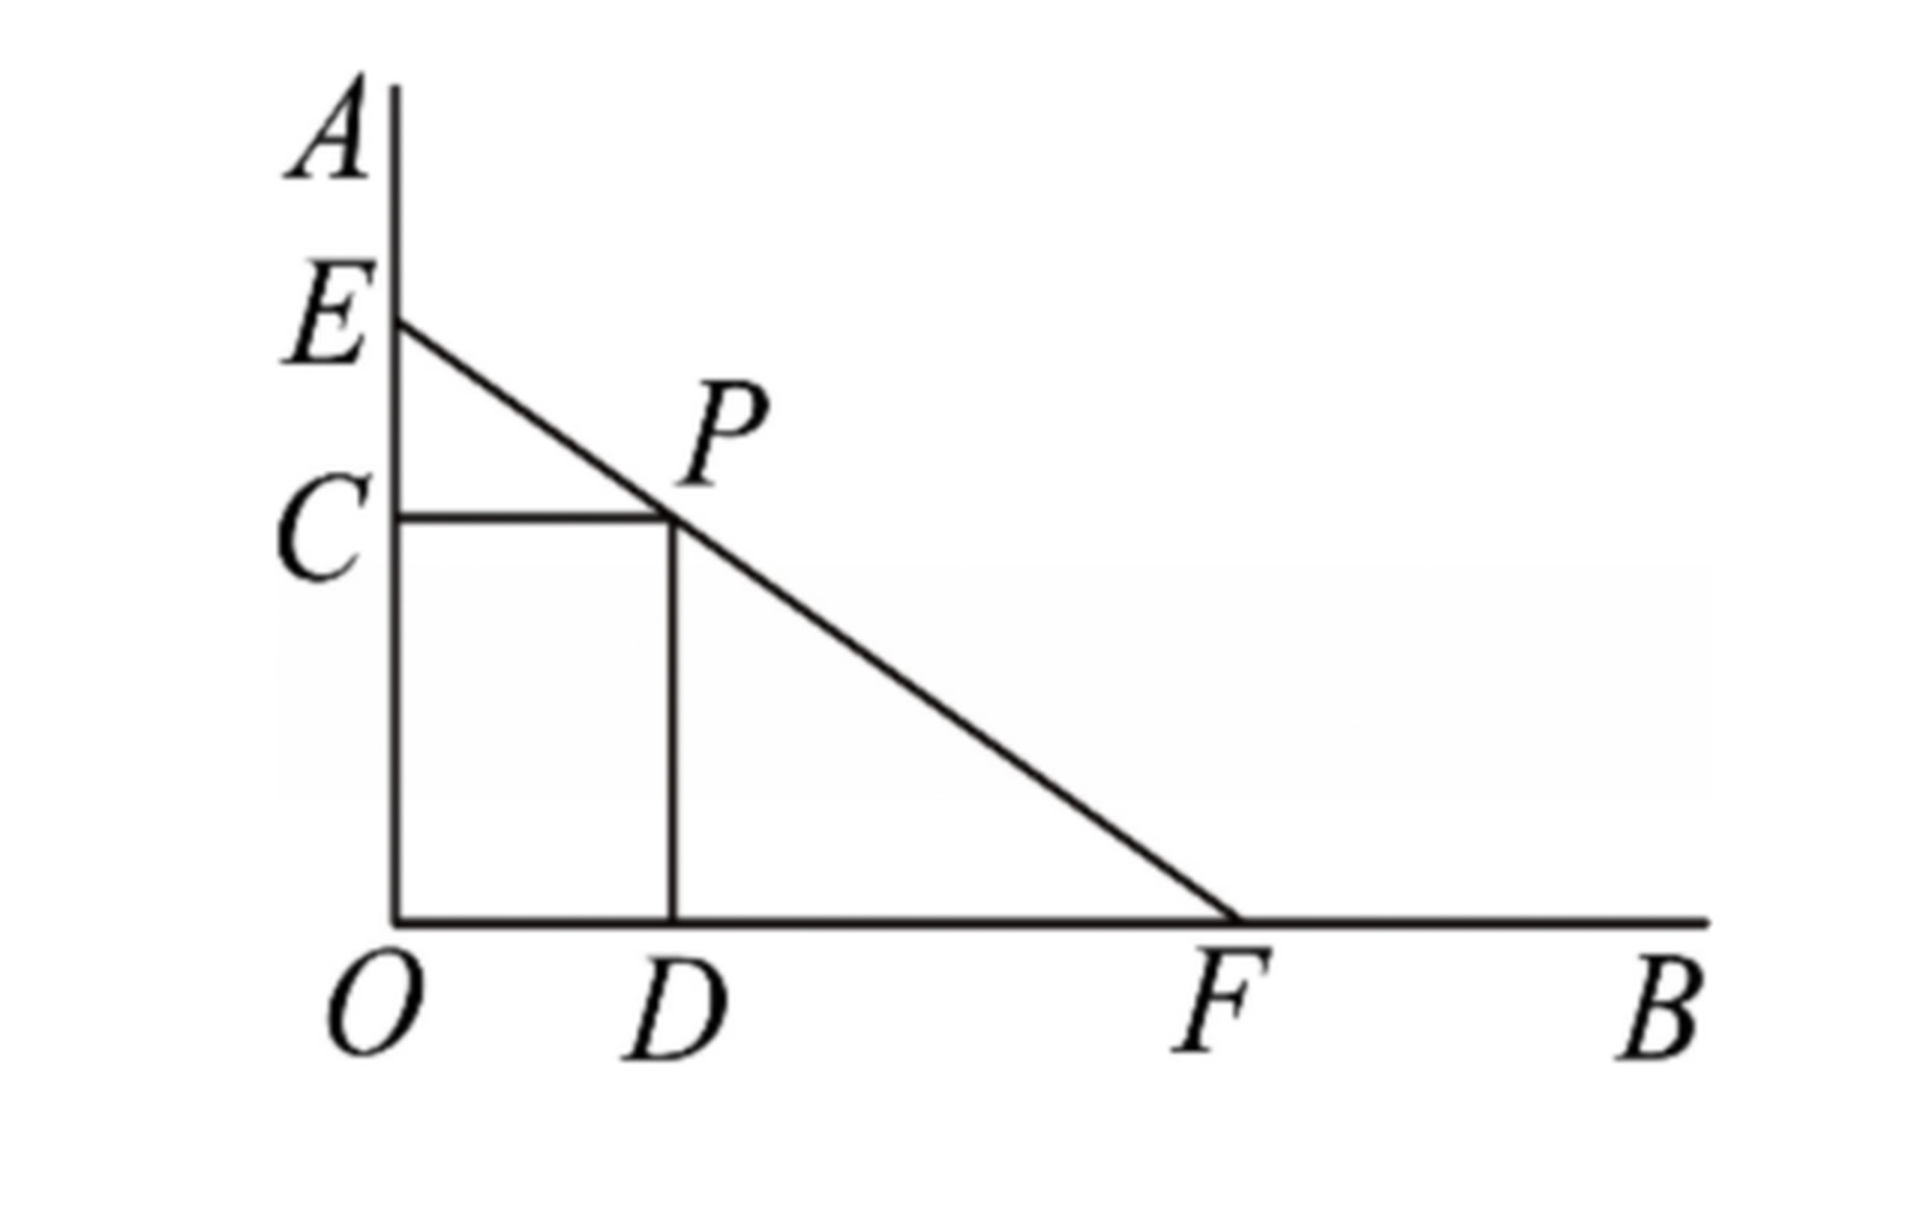
\includegraphics[width=0.32\textwidth]{figures/gao132_q18.png}
\end{center}

\ifanswer
\solbegin
\step{(1) 由题意得 $x\leq60$，}
\step{$\triangle PCE\sim\triangle FDP$，所以 $\dfrac{EC}{CP}=\dfrac{PD}{DF}$，即 $\dfrac{x}{25}=\dfrac{40}{DF}$，得 $DF=\dfrac{1000}{x}$m，}
\step{所以 $OF=OD+DF=\left(25+\dfrac{1000}x\right)$m，}
\step{所以 $25+\dfrac{1000}x\leq100$，解得 $x\geq\dfrac{40}3$；}
\step{综上，$\dfrac{40}3\leq x\leq60$；}
\step{(2) 由 $OE=OC+CE=(40+x)$m，}
\step{所以 $S=\dfrac12 OF\cdot OE=\dfrac12\left(25+\dfrac{1000}x\right)(40+x)$}
\step{$=\dfrac12\left(1000+25x+\dfrac{40000}x+1000\right)$m$^2$，}
\step{由基本不等式得 $S\geq\dfrac12\left(2000+2\sqrt{25x\cdot\dfrac{40000}x}\right)=2000$m$^2$，}
\step{当且仅当 $25x=\dfrac{40000}x$，即 $x=40$ 时取等号，}
\step{故 $EC=40$m 时，$S$ 取得最小值，为 $2000$m$^2$.}
\solend
\fi

\item 已知 $a>0$，$b>0$，请选择适当的方法证明.

(1) 若 $a\ne b$，证明：$a^3+b^3>a^2b+ab^2$；

(2) 若 $ab=1$，证明：$a^2+a<2$ 与 $b^2+b<2$ 不能同时成立.

\ifanswer
\solbegin
\step{(1) 因为 $a>0$，$b>0$，$a\ne b$，}
\step{所以 $a^3+b^3-a^2b-ab^2=a^2(a-b)+b^2(b-a)$}
\step{$=(a^2-b^2)(a-b)=(a-b)^2(a+b)>0$，所以 $a^3+b^3>a^2b+ab^2$.}
\step{(2) 假设 $a^2+a<2$ 与 $b^2+b<2$ 同时成立，所以 $-2<a<1,-2<b<1$，}
\step{又因为 $a>0,b>0$，所以 $0<a<1,0<b<1$，}
\step{所以 $0<ab<1$，这与 $ab=1$ 矛盾，}
\step{故 $a^2+a<2$ 与 $b^2+b<2$ 不可能同时成立.}
\solend
\fi

\item 若设 $M(a,n)=\lvert ax-1\rvert+\lvert ax-2\rvert+\cdots+\lvert ax-n\rvert$ 为曼哈顿扩张距离，它由 $n$ 个绝对值之和组成，其中 $n$ 为正整数.

(1) 若 $M(2,1)\leq5$，求 $x$ 的取值范围；

(2) 若 $k\leq M(2,2)$ 对一切实数 $x$ 恒成立，求实数 $k$ 的取值范围；

(3) $M(2,6)$ 是否存在最小值？若存在，求出该最小值与此时实数 $x$ 的取值范围；若不存在，说明理由.

\ifanswer
\solbegin
\step{(1) $M(2,1)=\lvert2x-1\rvert\leq5$，则不等式可化为 $-5\leq2x-1\leq5$，解得 $-2\leq x\leq3$，}
\step{所以 $x$ 的取值范围为 $[-2,3]$.}
\step{(2) 因为 $k\leq M(2,2)=\lvert2x-1\rvert+\lvert2x-2\rvert$ 对一切实数 $x$ 恒成立，}
\step{又 $\lvert2x-1\rvert+\lvert2x-2\rvert\geq\lvert(2x-1)-(2x-2)\rvert=1$，}
\step{当且仅当 $(2x-1)(2x-2)\leq0$，即 $\dfrac12\leq x\leq1$ 时取等号，}
\step{故 $k\leq1$，所以实数 $k$ 的取值范围为 $(-\infty,1]$.}
\step{(3) $M(2,6)=\lvert2x-1\rvert+\lvert2x-2\rvert+\lvert2x-3\rvert+\lvert2x-4\rvert+\lvert2x-5\rvert+\lvert2x-6\rvert$}
\step{$=2\left(\left\lvert x-\dfrac12\right\rvert+\lvert x-1\rvert+\left\lvert x-\dfrac32\right\rvert+\lvert x-2\rvert+\left\lvert x-\dfrac52\right\rvert+\lvert x-3\rvert\right)$，}
\step{其中 $\left\lvert x-\dfrac12\right\rvert+\lvert x-1\rvert+\left\lvert x-\dfrac32\right\rvert+\lvert x-2\rvert+\left\lvert x-\dfrac52\right\rvert+\lvert x-3\rvert$ 的几何意义为}
\step{在数轴上一点 $x$ 到 $\dfrac12,1,\dfrac32,2,\dfrac52,3$ 的距离之和，}
\step{要想距离之和最小，其中 $x\in\left[\dfrac12,3\right]$ 时，$\left\lvert x-\dfrac12\right\rvert+\lvert x-3\rvert$ 取得最小值，}
\step{当 $x\in\left[1,\dfrac52\right]$ 时，$\lvert x-1\rvert+\left\lvert x-\dfrac52\right\rvert$ 取得最小值，}
\step{当 $x\in\left[\dfrac32,2\right]$ 时，$\left\lvert x-\dfrac32\right\rvert+\lvert x-2\rvert$ 取得最小值，}
\step{综上，当 $x\in\left[\dfrac32,2\right]$ 时，$\left\lvert x-\dfrac12\right\rvert+\lvert x-1\rvert+\left\lvert x-\dfrac32\right\rvert+\lvert x-2\rvert+\left\lvert x-\dfrac52\right\rvert+\lvert x-3\rvert$}
\step{取得最小值，最小值为 $3-\dfrac12+\dfrac52-1+2-\dfrac32=\dfrac92$，}
\step{故 $M(2,6)=2\left(\left\lvert x-\dfrac12\right\rvert+\lvert x-1\rvert+\left\lvert x-\dfrac32\right\rvert+\lvert x-2\rvert+\left\lvert x-\dfrac52\right\rvert+\lvert x-3\rvert\right)$ 的}
\step{最小值为 $9$.}
\solend
\fi

\item 已知集合 $A=\{a_1,a_2,\cdots,a_n\}(0\leq a_1<a_2<\cdots<a_n,n\in\N,n\geq3)$ 具有性质 $Q$：对任意 $i,j(1\leq i\leq j\leq n)$，$a_i+a_j$ 与 $a_j-a_i$ 至少有一个属于集合 $A$；

(1) 判断集合 $M=\{0,2,4\}$ 与 $N=\{2,3,4\}$ 是否具有性质 $Q$，并说明理由；

(2) 已知 $A=\{a_1,a_2,a_3\}$ 具有性质 $Q$，当 $a_2=2026$ 时，求集合 $A$；

(3) 已知 $B=\{b_1,b_2,\cdots,b_{2026}\}$ 具有性质 $Q$，求 $\dfrac{b_1+b_2+\cdots+b_{2026}}{b_{2026}}$ 的值；

\ifanswer
\solbegin
\step{(1) 集合 $M=\{0,2,4\}$ 中，}
\step{因为 $0+2\in M,0+4\in M,4-2\in M,0\pm0=0\in M$，}
\step{$2+2=4\in M,2-2=0\in M,4-4=0\in M$，所以集合 $M$ 具有性质 $Q$；}
\step{集合 $N=\{2,3,4\}$ 中，因为 $3+3=6\notin N,3-3=0\notin N$，}
\step{所以集合 $N$ 不具有性质 $Q$.}
\step{(2) 因为 $a_1<a_2<a_3$，且 $A=\{a_1,a_2,a_3\}$ 具有性质 $Q$，}
\step{所以 $a_3+a_3\notin A,a_3-a_3=0\in A$，则 $a_1=0$，}
\step{又因为 $a_2+a_3>a_3$，所以 $a_2+a_3\notin A$，则 $a_3-a_2\in A$，}
\step{由集合的互异性得 $a_3-a_2=a_2$，而 $a_2=2026$，所以 $a_3=4052$，}
\step{故 $A=\{0,2026,4052\}$；}
\step{(3) 先证明一般结论：$A=\{a_1,a_2,\cdots,a_n\}(0\leq a_1<a_2<\cdots<a_n,n\in\N,n\geq3)$}
\step{具有性质 $Q$，则 $a_1+a_2+a_3+\cdots+a_n=\dfrac n2 a_n$.}
\step{因为 $A=\{a_1,a_2,\cdots,a_n\}(0\leq a_1<a_2<\cdots<a_n,n\in\N,n\geq3)$ 具有性质 $Q$，}
\step{所以 $a_n+a_n\notin A$，则 $a_n-a_n=0\in A$，则 $a_1=0$.}
\step{又因为 $0\leq a_1<a_2<\cdots<a_n$，所以 $0\leq a_n-a_n<a_n-a_{n-1}<\cdots<a_n-a_1$，}
\step{又因为 $a_n+a_{n-i}>a_n(i=1,2,\cdots,n-1)$，所以 $a_n+a_{n-i}\notin A$，}
\step{则 $a_n-a_{n-i}\in A$，}
\step{所以 $a_1=a_n-a_n,a_2=a_n-a_{n-1},a_3=a_n-a_{n-2},\cdots,a_n=a_n-a_1$.}
\step{所以 $a_1+a_2+a_3+\cdots+a_n$}
\step{$=(a_n-a_n)+(a_n-a_{n-1})+(a_n-a_{n-2})+\cdots+(a_n-a_1)$，}
\step{即 $a_1+a_2+a_3+\cdots+a_n=\dfrac n2 a_n$，}
\step{所以 $B=\{b_1,b_2,\cdots,b_{2026}\}$ 具有性质 $Q$，则 $b_1+b_2+\cdots+b_{2026}=\dfrac{2026}{2}b_{2026}$，}
\step{所以 $\dfrac{b_1+b_2+\cdots+b_{2026}}{b_{2026}}=\dfrac{2026}{2}=1013$.}
\solend
\fi

\end{enumerate}

% 行数复核：逐题数 \step 条数，合计 144 条（Q3：4；Q4：1；Q5：4；Q6：2；Q7：9；Q8：2；
% Q9：3；Q10：6；Q11：9；Q12：9；Q13：0；Q14：9；Q15：4；Q16：19；Q17：5；Q18：11；
% Q19：7；Q20：17；Q21：23），与原卷印刷行逐题相等（cases 块作一个印刷行计）。
% 第 13 题只印括号内答案、提 \ans{}，不计入 \step 账；第 14—16 题答案在解析末句，
% 括号内留空、不另提 \ans{}。

\end{document}
"
%
% 原始材料：微信公众号"魔都数学加油站"文章，作者破晓，2026-11-14 19:00 发布；
% 连载"27学年高一132"，原文标题"27学年高一132——2026-2027年上海市川沙中学高一上期中"；
% 原文链接：https://mp.weixin.qq.com/s/VBG01CrUNMIYWWHhSfz8JQ。
% 正文为 11 张 PNG 页（01、04、06、07、09、11 为 2560x3620，02、03、05、08、10 为 4762x6735），
% 题目下印有【解析】，为讲评版。题目、解析均据原图转录；
% 卷面粉红色水印"魔都数学加油站"及公众号页脚未录入。全卷 2 幅插图：第 14 题四幅坐标图选项、
% 第 18 题矩形 OCPD 与小路 EF 示意图，均取原卷 04／07 页截图去水印。
%
% 卷首标题：原卷印作"2026-2027 年川沙中学高一上期中"（公众号标题中的"上海市"
% 卷面标题行没有，本稿照卷面），年份区间按全稿惯例排 en dash；原卷未印副标题，
% 本卷为期中卷、跨集合与常用逻辑用语／不等式／函数三章，按题目内容标为
% "集合与常用逻辑用语、不等式、函数"（与 125／126／128／129／131 同期中卷口径相同）：
% 集合与逻辑见 Q5、Q6、Q17、Q21，不等式见 Q3、Q4、Q9、Q10、Q12、Q13、Q15、Q16、Q19，
% 函数（幂函数、指数／对数、基本不等式应用）见 Q7、Q8、Q11、Q14、Q18、Q20。
%
% 题号体例：本卷共 19 题——一、填空题 3—12（10 题）、二、选择题 13—16（4 题）、
% 三、解答题 17—21（5 题）。三节分别 \setcounter{enumi}{2}／{12}／{16}。
%
% 与原卷的排版差异：
%   ① 原文从第 3 题起，本稿保留原题号（见上"题号体例"）；
%   ② 原卷每题下直接印【解析】，本稿按全稿惯例置于答案版；第 13 题答案 D 印在题干
%      括号内、无独立答案段，按 高一37／52／53／55／63／64／128／131 成例括号留空、
%      另提 \ans{$D$}；第 14—16 题答案在解析末句"故选 …"，括号内留空、不另提 \ans{}；
%   ③ 原卷未印副标题，本稿按"知识模块"口径补出；
%   ④ 原卷填空横线按全稿惯例排为 \blankline[4.4em]；选择题括号排 \mbox{（\quad）}、
%      选项段前按惯例加 \keepwithprev；解答题不留作答区（原卷为讲评版，与 109—131 同）；
%   ⑤ 原卷数集排斜体 $R^+$／$R$／$Z$／$N$，按全稿惯例改 \R^+／\R／\Z／\N；
%      绝对值排 \lvert…\rvert，集合描述竖线排 \mid；不等号按全稿惯例排 \leqslant／\geqslant；
%      补集照原卷上划线排 \overline{B}；
%   ⑥ 子题标号 (1)(2)(3) 原卷用半角括号，照录；第 14 题四幅坐标图选项按原卷 2×2 排布
%      合并裁为一张 \includegraphics（未用 TikZ 重绘，以保证与原卷一致），题前加
%      \needvspace{9cm} 守卫；第 18 题图取 07 页截图，题前按惯例加 \needvspace{7cm} 守卫
%      （照 高一120／127／129／131 成例），两者守卫都放在 \item 之前；
%   ⑦ 原卷 Q7 解析跨 01—02 页、Q10 解析跨 02—03 页、Q12 解析跨 03—04 页、
%      Q14 解析跨 04—05 页、Q16 解析在 06 页、Q18 解析跨 07—08 页、
%      Q20 解析跨 08—09 页、Q21 解析跨 10—11 页，本稿按题合并连续排版；
%      末页第 11 页为 Q21 (3) 解析的续尾，按实际印刷行单列。
%
% 判别式字形：第 10 题 $\triangle=4(a-1)^2+16(a-1)<0$、第 11 题
%   $\triangle=4(m-2)^2-4(m^2-3m+3)=-4m+4>0$ 两处原卷均排 $\triangle$（等边、扁），
%   逐处放大核对、字形一致，照录 \triangle；与 高一129／131 同题排 $\Delta$（等腰、高）不同。
%   全卷 \triangle 兼作第 18 题「$\triangle PCE\sim\triangle FDP$」「$\triangle OEF$」的几何
%   三角形记号，全卷未出现 \Delta。
%
% 子集符号：第 5 题解析 $B\subseteq A$、第 17 题 (2) 解析 $A\subseteq B$ 均印带下划线，
%   照录 \subseteq；全卷未出现单线 \subset。
%
% 原卷存疑照录：
%   第 9 题题干作"充分非必要条件"、解析作"充分不必要条件"，措辞不同，照录；
%   第 10 题解析"当 $a-1=0$ 时，$-4\geq0$，不等式不成立，$a=1$ 满足题意"照录；
%   第 11 题解析"所以 $2(m-1)+\dfrac1{m-1}\leq-2\sqrt2$"由上一行 $2(1-m)+\dfrac1{1-m}\geq2\sqrt2$
%     直接变号得到，照录；
%   第 12 题解析"由 $x\in Z$，$-7<-2\sqrt{10}<-6$"与"即 $k^2+7k+10\leq0$，解得 $-5\leq k\leq-2$"照录；
%   第 16 题解析"令 $52\times(930+a)=-52$，解得 $a=-931$"（按式应为 $a=-931$ 之外的解）照录；
%   第 19 题 (2) 解析"所以 $-2<a<1,-2<b<1$"数学式内半角逗号，照录；
%   第 20 题 (3) 解析"最小值为 $3-\dfrac12+\dfrac52-1+2-\dfrac32=\dfrac92$"与
%     "故 $M(2,6)=\dots$ 的最小值为 9"两处结论并列，照录；
%   第 21 题 (1) 解析"$0+2\in M,0+4\in M,4-2\in M,0\pm0=0\in M$"、
%     "$2+2=4\in M,2-2=0\in M,4-4=0\in M$"、(3) 各连写等式内半角逗号，照录；
%   第 21 题 (3) 解析"即 $a_1+a_2+a_3+\cdots+a_n=\dfrac n2 a_n$，"句末用半角逗号，照录。
%
% 行数复核：见文末"行数复核"注（逐题 \step 条数与原卷印刷行逐题相等，cases 块作一个印刷行计）。
%   第 13 题只印括号内答案、提 \ans{}，不计入 \step 账；第 14—16 题答案在解析末句，
%   括号内留空、不另提 \ans{}。
%
\documentclass[a4paper,11pt]{article}
\usepackage{common}

\begin{document}

\examtitlest[3]{2026--2027 年川沙中学高一上期中}{集合与常用逻辑用语、不等式、函数}

\bigsec{一、填空题}

\begin{enumerate}
\setcounter{enumi}{2}

\item 已知 $a$、$b\in\R^+$ 且 $ab=2$，则 $a+2b$ 的最小值为\blankline[4.4em].

\ifanswer
\solbegin
\step{因为 $a\in\R^+$，$b\in\R^+$ 且 $ab=2$，}
\step{由基本不等式得 $a+2b\geq2\sqrt{a\cdot2b}=2\sqrt{2ab}=2\sqrt4=4$.}
\step{等号当且仅当 $a=2b$ 时成立，结合 $ab=2$ 解得 $b=1$，$a=2$，}
\step{所以 $a+2b$ 的最小值为 $4$.}
\solend
\fi

\item 如果幂函数 $f(x)=(m^2-3m-3)x^{m^2+m-3}$ 在 $(0,+\infty)$ 上是增函数，则实数 $m=$\blankline[4.4em].

\ifanswer
\solbegin
\step{由已知得 $\begin{cases}m^2-3m-3=1\\m^2+m-3>0\end{cases}$，所以 $m=4$.}
\solend
\fi

\item 已知集合 $A=\{1,2\}$，集合 $B=\{x\mid ax=6\}$，若 $A\cup B=A$，则 $a$ 的所有取值构成的集合为\blankline[4.4em].

\ifanswer
\solbegin
\step{因为 $A\cup B=A$，所以 $B\subseteq A$，}
\step{当 $a=0$ 时，$B=\varnothing$，满足 $B\subseteq A$；}
\step{当 $a\ne0$ 时，$B=\left\{\dfrac6a\right\}$，则 $\dfrac6a=1$ 或 $\dfrac6a=2$，解得 $a=6$ 或 $a=3$，}
\step{综上所述，$a$ 的所有取值构成的集合为 $\{0,3,6\}$.}
\solend
\fi

\item 设全集为 $\R$，$A=\{y\mid y=-x^2+2x+1\}$，$B=\{x\mid y=\ln(x-1)\}$，则 $A\cap B=$\blankline[4.4em].

\ifanswer
\solbegin
\step{$A=\{y\mid y=-x^2+2x+1\}=\{y\mid y=-(x-1)^2+2\}=\{y\mid y\leq2\}$，}
\step{$B=\{x\mid y=\ln(x-1)\}=\{x\mid x>1\}$，则 $A\cap B=(1,2]$.}
\solend
\fi

\item 已知 $x\in\R$，则方程 $\lvert 6-x\rvert+\lvert 6x-3\rvert=\lvert 5x+3\rvert$ 的解集为\blankline[4.4em].

\ifanswer
\solbegin
\step{当 $x<-\dfrac35$ 时，$6-x>0$，$6x-3<0$，$5x+3<0$，}
\step{原方程为 $6-x-6x+3=-5x-3$，解得 $x=6$，不满足 $x<-\dfrac35$；}
\step{当 $-\dfrac35\leq x\leq\dfrac12$ 时，$5x+3\geq0$，$6x-3<0$，$6-x>0$，}
\step{原方程为 $6-x+3-6x=5x+3$，解得 $x=\dfrac12$；}
\step{当 $\dfrac12<x\leq6$ 时，$5x+3>0$，$6x-3>0$，$6-x\geq0$，}
\step{原方程为 $6-x+6x-3=5x+3$，即 $0=0$，恒成立，所以 $\dfrac12<x\leq6$；}
\step{当 $x>6$ 时，$5x+3\geq0$，$6x-3>0$，$6-x<0$，}
\step{原方程为 $x-6+6x-3=5x+3$，解得 $x=6$，不满足 $x>6$；}
\step{综上 $\dfrac12\leq x\leq6$，所以原方程的解集为 $\left\{x\mid\dfrac12\leq x\leq6\right\}$.}
\solend
\fi

\item 已知 $\log_2 3=a,2^b=7$，用 $a,b$ 表示 $\log_{42}56$ 为\blankline[4.4em].

\ifanswer
\solbegin
\step{$\log_{42}56=\dfrac{\log_2 56}{\log_2 42}=\dfrac{\log_2(7\times8)}{\log_2(6\times7)}=\dfrac{\log_2 7+\log_2 8}{\log_2 6+\log_2 7}$}
\step{$=\dfrac{\log_2 7+\log_2 2^3}{\log_2 2+\log_2 3+\log_2 7}=\dfrac{b+3}{1+a+b}$.}
\solend
\fi

\item 已知 $\dfrac13<x<\dfrac12$ 是不等式 $\lvert x-m\rvert<1$ 成立的充分非必要条件，则 $m$ 的取值范围是\blankline[4.4em].

\ifanswer
\solbegin
\step{因为 $\lvert x-m\rvert<1$，所以 $-1<x-m<1$，所以 $m-1<x<m+1$，}
\step{所以 $m-1<x<m+1$ 成立的充分不必要条件是 $\dfrac13<x<\dfrac12$，}
\step{所以 $\begin{cases}m-1\leq\dfrac13\\m+1\geq\dfrac12\end{cases}$，解得 $-\dfrac12\leq m\leq\dfrac43$，故 $m$ 的取值范围是 $\left[-\dfrac12,\dfrac43\right]$.}
\solend
\fi

\item 若关于 $x$ 的不等式 $(a-1)x^2+2(a-1)x-4\geq0$ 的解集为空集，则 $a$ 的取值范围是\blankline[4.4em].

\ifanswer
\solbegin
\step{关于 $x$ 的不等式 $(a-1)x^2+2(a-1)x-4\geq0$ 的解集为 $\varnothing$，}
\step{当 $a-1=0$ 时，$-4\geq0$，不等式不成立，$a=1$ 满足题意；}
\step{当 $a-1>0$ 时，$a>1$，不等式的解集不为空集，不满足题意；}
\step{当 $a-1<0$ 时，$a<1$，当 $\triangle=4(a-1)^2+16(a-1)<0$ 时，即 $(a-1)(a+3)<0$，}
\step{解得 $-3<a<1$，满足题意；}
\step{综上，实数 $a$ 的取值范围是 $\{a\mid-3<a\leq1\}$.}
\solend
\fi

\item 已知关于 $x$ 的方程 $x^2+2(m-2)x+m^2-3m+3=0$ 有两个不相等的实数根 $x_1$、$x_2$，则 $\dfrac{mx_1}{x_1-1}+\dfrac{mx_2}{x_2-1}-\dfrac{2}{x_1+x_2-2}$ 的最大值为\blankline[4.4em].

\ifanswer
\solbegin
\step{关于 $x$ 的方程 $x^2+2(m-2)x+m^2-3m+3=0$ 有两个不相等的实数根 $x_1$、$x_2$，}
\step{则 $\triangle=4(m-2)^2-4(m^2-3m+3)=-4m+4>0$，得 $m<1$，}
\step{且 $x_1+x_2=-2(m-2)$，$x_1x_2=m^2-3m+3$，}
\step{$\dfrac{mx_1}{x_1-1}+\dfrac{mx_2}{x_2-1}-\dfrac{2}{x_1+x_2-2}=\dfrac{m[2x_1x_2-(x_1+x_2)]}{x_1x_2-(x_1+x_2)+1}+\dfrac1{m-1}$}
\step{$=\dfrac{2m(m-1)^2}{m^2-m}+\dfrac1{m-1}=2(m-1)+\dfrac1{m-1}$，}
\step{又因为 $m<1$，所以 $m-1<0$，则 $1-m>0$，}
\step{所以 $2(1-m)+\dfrac1{1-m}\geq2\sqrt{2(1-m)\cdot\dfrac1{1-m}}=2\sqrt2$，}
\step{当且仅当 $2(1-m)=\dfrac1{1-m}$ 时，即 $m=1-\dfrac{\sqrt2}2$ 时取等号，}
\step{所以 $2(m-1)+\dfrac1{m-1}\leq-2\sqrt2$，即 $\dfrac{mx_1}{x_1-1}+\dfrac{mx_2}{x_2-1}-\dfrac2{x_1+x_2-2}$ 的最大值为 $-2\sqrt2$.}
\solend
\fi

\item 若使集合 $A=\{x\mid(kx-k^2-10)(x-1)>0,x\in\Z\}$ 中的元素个数最少，则实数 $k$ 的取值范围是\blankline[4.4em].

\ifanswer
\solbegin
\step{由题意集合 $A=\{x\mid(kx-k^2-10)(x-1)>0,\ x\in\Z\}$，}
\step{$k=0$ 时，不等式解得 $x<1$，有无数个整数解；}
\step{$k\ne0$ 时，则不等式变形为 $k\left(x-k-\dfrac{10}k\right)(x-1)>0$，}
\step{当 $k>0$ 时，$k+\dfrac{10}k\geq2\sqrt{10}$，仅当 $k=\sqrt{10}$ 时等号成立，}
\step{此时不等式解得 $x>k+\dfrac{10}k$ 或 $x<1$，有无数个整数解；}
\step{当 $k<0$ 时，$k+\dfrac{10}k=-\left[(-k)+\left(-\dfrac{10}k\right)\right]\leq-2\sqrt{10}$，仅当 $k=-\sqrt{10}$ 时等号成立，}
\step{此时不等式解得 $k+\dfrac{10}k<x<1$，}
\step{由 $x\in\Z$，$-7<-2\sqrt{10}<-6$，要使集合 $A$ 中的元素最少，则 $k+\dfrac{10}k\geq-7$，}
\step{即 $k^2+7k+10\leq0$，解得 $-5\leq k\leq-2$，故实数 $k$ 的取值范围是 $[-5,-2]$.}
\solend
\fi

\end{enumerate}

\bigsec{二、选择题}

\begin{enumerate}
\setcounter{enumi}{12}

\item 下列说法正确的是\mbox{（\quad）}

\keepwithprev
A. 若 $a>b$，则 $\dfrac1a<\dfrac1b$\qquad\qquad B. 若 $a>b$，$c>d$，则 $ac>bd$

C. 若 $a>b$，则 $ac^2>bc^2$\qquad\qquad D. 若 $ac^2>bc^2$，则 $a>b$

\ifanswer
\ans{$D$}
\fi

% 第 14 题四幅坐标图选项是一整块，守卫放在 \item 之前
\needvspace{9cm}
\item 在同一坐标系内，函数 $y=x^a(a\ne0)$ 和 $y=ax-\dfrac1a$ 的图象可能是\mbox{（\quad）}

\keepwithprev
\begin{center}
% 四幅坐标图选项取原卷 04 页截图去粉色水印，按原卷 2×2 排布合并为一张
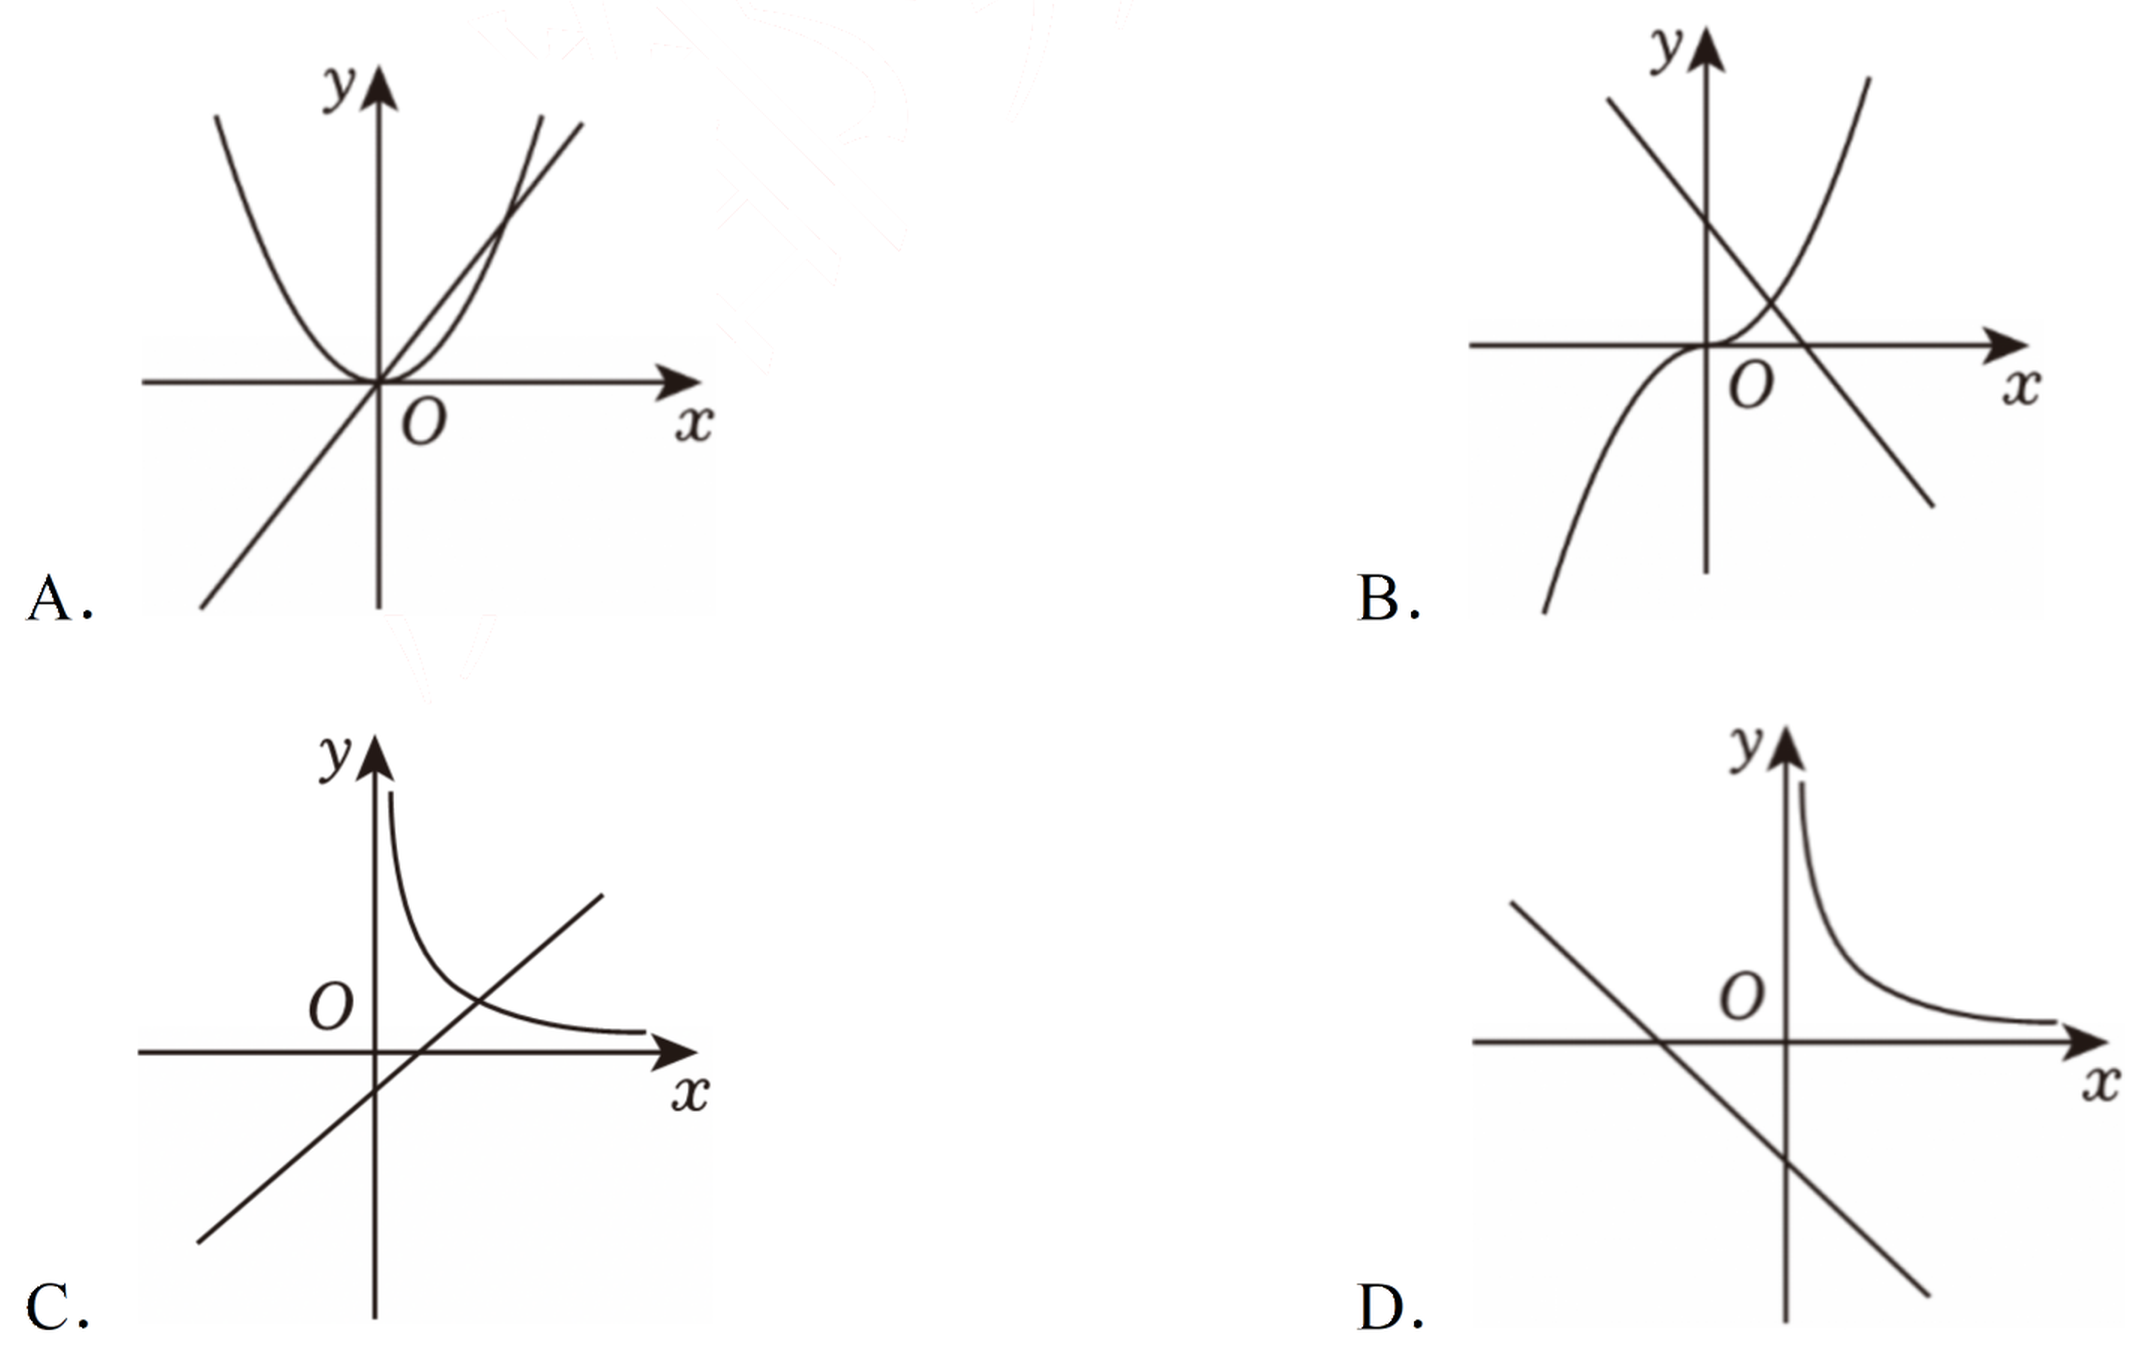
\includegraphics[width=0.80\textwidth]{figures/gao132_q14.png}
\end{center}

\ifanswer
\solbegin
\step{当 $a>0$ 时，$y=ax-\dfrac1a$ 严格增，当 $a<0$ 时，$y=ax-\dfrac1a$ 严格减，}
\step{对于 $A$，因为 $a\ne0$，所以直线 $y=ax-\dfrac1a$ 不过原点，故 $A$ 错误；}
\step{对于 $B$，由函数 $y=x^a(a\ne0)$ 的图象得 $a>1$，}
\step{由 $y=ax-\dfrac1a$ 的图象得 $a<0$，互相矛盾，故 $B$ 错误；}
\step{对于 $C$，由函数 $y=x^a(a\ne0)$ 的图象得 $a>1$，}
\step{由 $y=ax-\dfrac1a$ 的图象得 $a>0$ 且 $-\dfrac1a<0$，符合题意，故 $C$ 正确；}
\step{对于 $D$，由函数 $y=x^a(a\ne0)$ 的图象得 $a<0$，}
\step{由 $y=ax-\dfrac1a$ 的图象得 $a<0$ 且 $-\dfrac1a<0$，互相矛盾，故 $D$ 错误；}
\step{故选 $C$.}
\solend
\fi

\item 中国的 $5G$ 技术领先世界，在 $5G$ 技术中，最大数据传输速率 $C$ 取决于信道带宽 $W$，$C$ 与 $W$ 满足 $C=W\log_2\left(1+\dfrac SN\right)$，其中 $\dfrac SN$ 称为信噪比（单位：$dB$）. 若不改变带宽 $W$，初始信噪比 $\dfrac SN$ 为 $1000$，那么为了使 $C$ 增加 $30\%$，需要将信噪比 $\dfrac SN$ 从 $1000$ 提升至大约\mbox{（\quad）}

\keepwithprev
A. $5000$\qquad\qquad B. $6000$\qquad\qquad C. $7000$\qquad\qquad D. $8000$

\ifanswer
\solbegin
\step{由题意得 $\dfrac SN=1000$ 时，$C=W\log_2(1+1000)\approx W\log_2 1000$，}
\step{要使 $C$ 增加 $30\%$，则 $(1+30\%)C=W\log_2\left(1+\dfrac SN\right)$，即 $1.3C\approx W\log_2\dfrac SN$，}
\step{所以 $1.3\approx\log_{1000}\dfrac SN=\dfrac{\lg\frac SN}{\lg1000}$，所以 $\lg\dfrac SN=3.9$，所以 $\dfrac SN=10^{3.9}\approx8000$.}
\step{故选 $D$.}
\solend
\fi

\item 对于 $a\in\R$，设非空集合 $A=\left\{x\mid\dfrac{(x^2-930x+a)(x-52)}{x+a}=0\right\}$，记 $A$ 中的所有元素之和为 $S(a)$，所有元素之积为 $T(a)$，则下列说法中，不正确的是\mbox{（\quad）}

\keepwithprev
A. 存在实数 $a$，使得 $S(a)=930$

B. 存在实数 $a$，使得 $T(a)=517$

C. 不存在实数 $a$，使得 $T(a)=0$

D. 恰存在 $1$ 个实数 $a$，使得 $T(a)=-52$

\ifanswer
\solbegin
\step{由分式值为 $0$，得分子为 $0$ 且分母不为 $0$，}
\step{分子 $(x^2-930x+a)(x-52)=0$ 的根为 $x=52$}
\step{及方程 $x^2-930x+a=0$ 的两根 $x_1$，$x_2$，}
\step{由根与系数的关系得 $x_1+x_2=930$，$x_1\cdot x_2=a$，}
\step{分母限制 $x\ne-a$，需要剔除等于 $-a$ 的根，}
\step{选项 $A$，取 $a=-52$，$x=52$ 为增根舍去，集合 $A=\{x_1,x_2\}$，}
\step{元素之和 $S(a)=930$，故 $A$ 正确；}
\step{选项 $B$，当无增根时，$T(a)=52a$，令 $52a=517$，得 $a=\dfrac{517}{52}$，}
\step{验证无增根，存在这样的 $a$，故 $B$ 正确；}
\step{选项 $C$，若 $T(a)=0$，则 $0\in A$，代入分子得 $a=0$，}
\step{但 $a=0$ 时分母 $x\ne0$，$x=0$ 为增根，$0$ 不能属于集合 $A$，}
\step{故不存在 $a$ 使得 $T(a)=0$，故 $C$ 正确；}
\step{选项 $D$，当无增根时，令 $52a=-52$，得 $a=-1$；}
\step{当 $x=-a$ 是二次方程的根且不等于 $52$ 时，}
\step{令 $52\times(930+a)=-52$，解得 $a=-931$，验证符合条件；}
\step{当 $a=-52$ 时，$x=52$，舍去，}
\step{集合 $A=\{x_1,x_2\}$，$T(a)=a=-52$，得到两个满足条件的 $a$；}
\step{因此存在 $3$ 个满足条件的 $a$，故 $D$ 错误.}
\step{故选 $D$.}
\solend
\fi

\end{enumerate}

\bigsec{三、解答题}

\begin{enumerate}
\setcounter{enumi}{16}

\item 已知全集 $U=\R$，集合 $A=\left\{x\mid\dfrac{x}{x-3}<0\right\}$，$B=\{x\mid(x-a)(x+4-a)<0\}$.

(1) 当 $a=2$ 时，求 $\overline{B}$、$A\cap\overline{B}$；

(2) 若 $A\cap B=A$，求实数 $a$ 的取值范围.

\ifanswer
\solbegin
\step{(1) $\dfrac{x}{x-3}<0$，即 $x(x-3)<0$，解得 $A=\{x\mid0<x<3\}$，}
\step{当 $a=2$ 时，$B=\{x\mid(x-a)(x+4-a)<0\}=\{x\mid-2<x<2\}$，}
\step{则 $\overline{B}=\{x\mid x\leq-2$ 或 $x\geq2\}$，故 $A\cap\overline{B}=\{x\mid2\leq x<3\}$；}
\step{(2) $A\cap B=A$，则 $A\subseteq B$，故 $\begin{cases}a-4\leq0\\a\geq3\end{cases}$，解得 $3\leq a\leq4$，}
\step{故实数 $a$ 的取值范围是 $\{a\mid3\leq a\leq4\}$.}
\solend
\fi

% 第 18 题是"题干 + 图"约 7cm 的一整块，守卫放在 \item 之前
\needvspace{7cm}
\item 如图，$OA$、$OB$ 是两条长度足够长的互相垂直的笔直小路，矩形 $OCPD$ 的顶点 $C$、$D$ 分别在 $OA$、$OB$ 上，且该矩形区域内种满了荷花. 为了让观赏者有更好的观赏体验，现计划经过点 $P$ 修一条小路 $EF$，其中点 $E$ 在小路 $OA$ 上，点 $F$ 在小路 $OB$ 上，并在 $\triangle OEF$ 区域内种满荷花. 已知 $OD=25m$，$OC=40m$，且小路 $EF$ 要完全位于一个以 $O$ 为顶点的，边长为 $100$ m 的正方形内部（包括边界）. 记 $\triangle OEF$ 的面积为 $S$m$^2$.

(1) 设 $EC=x\cdot m$，试用 $x$ 表示 $OF$，并求 $x$ 的取值范围.

(2) 当 $EC$ 的长度为多少时，$S$ 取得最小值？最小值是多少？

\begin{center}
% 图取原卷 07 页截图去粉色水印，3× LANCZOS 放大
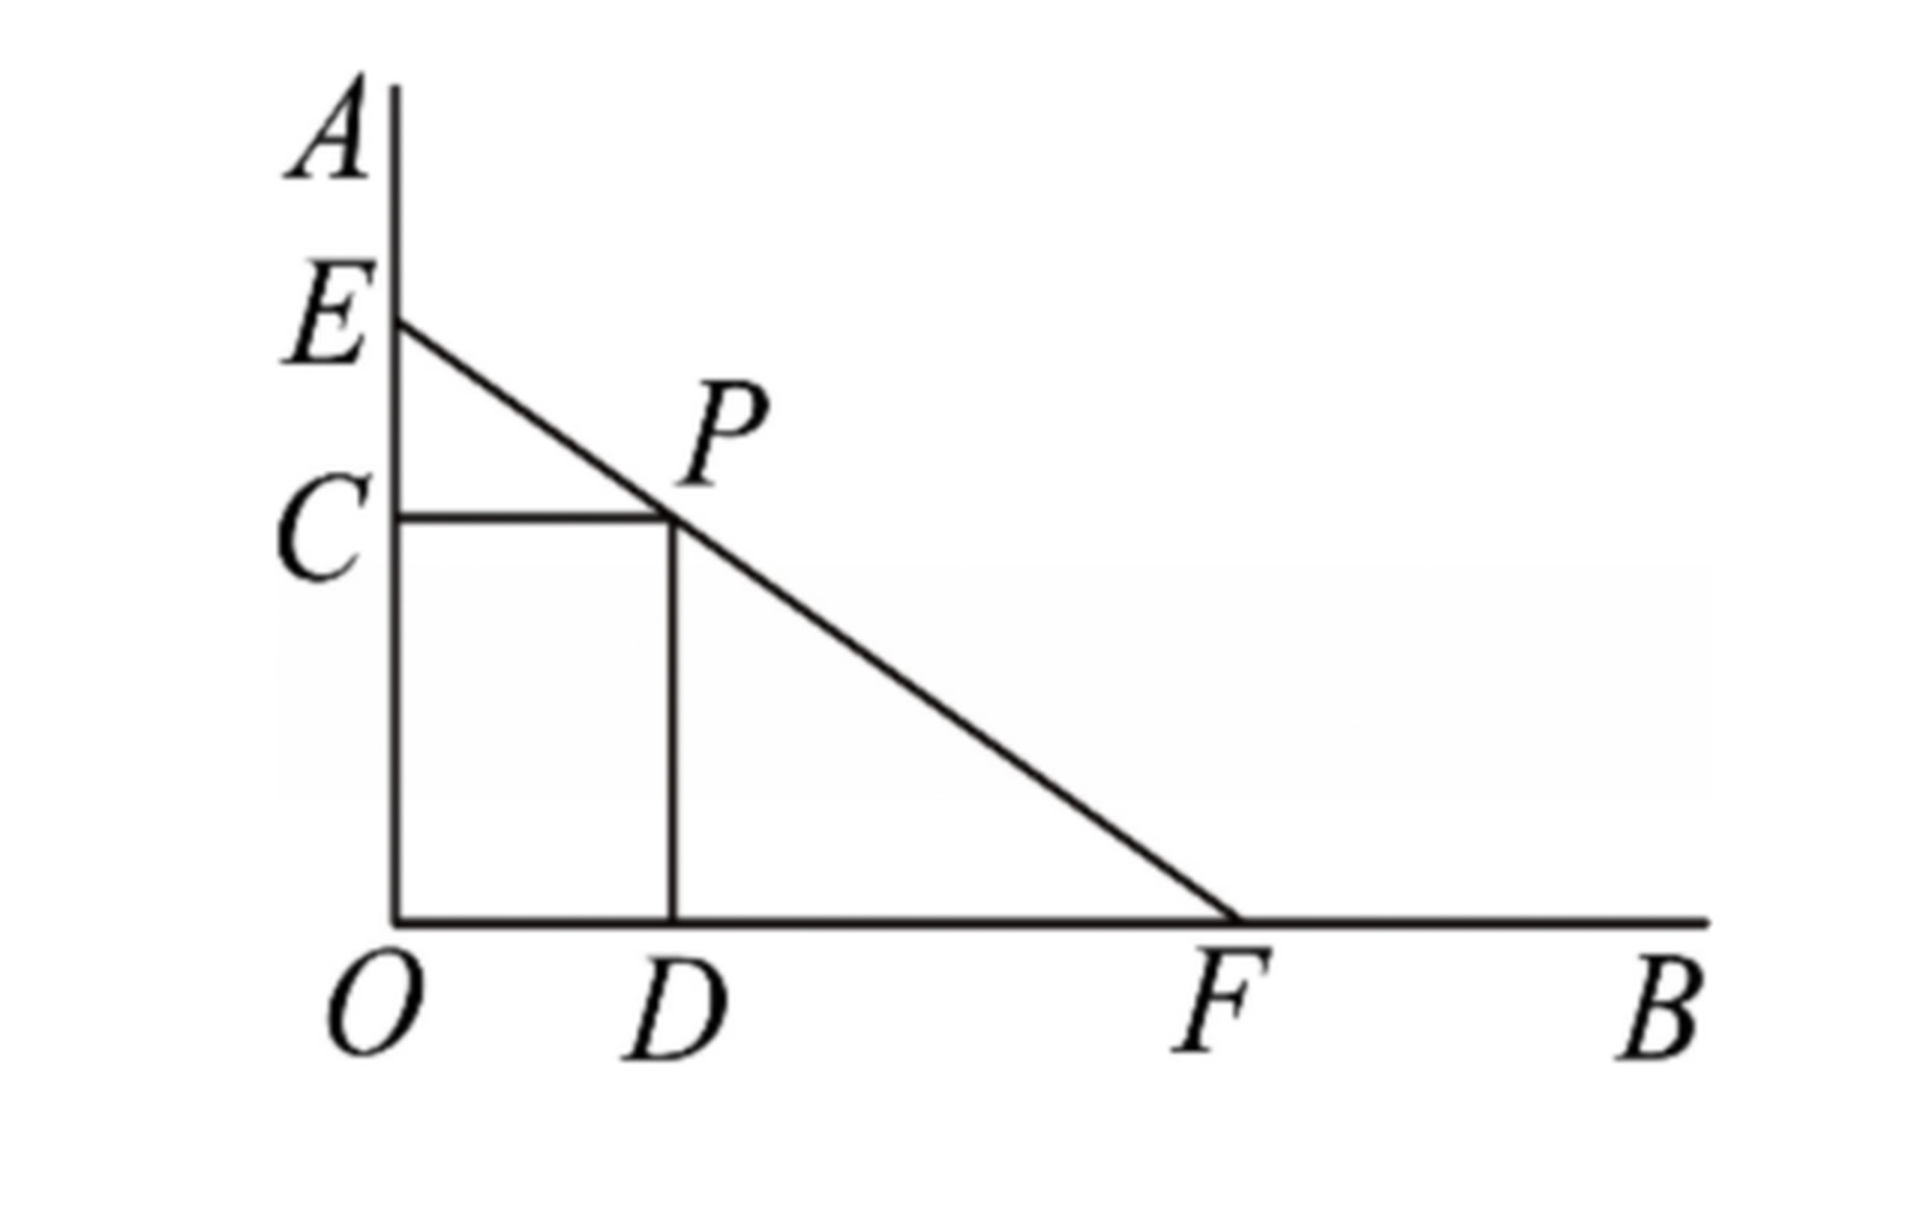
\includegraphics[width=0.32\textwidth]{figures/gao132_q18.png}
\end{center}

\ifanswer
\solbegin
\step{(1) 由题意得 $x\leq60$，}
\step{$\triangle PCE\sim\triangle FDP$，所以 $\dfrac{EC}{CP}=\dfrac{PD}{DF}$，即 $\dfrac{x}{25}=\dfrac{40}{DF}$，得 $DF=\dfrac{1000}{x}$m，}
\step{所以 $OF=OD+DF=\left(25+\dfrac{1000}x\right)$m，}
\step{所以 $25+\dfrac{1000}x\leq100$，解得 $x\geq\dfrac{40}3$；}
\step{综上，$\dfrac{40}3\leq x\leq60$；}
\step{(2) 由 $OE=OC+CE=(40+x)$m，}
\step{所以 $S=\dfrac12 OF\cdot OE=\dfrac12\left(25+\dfrac{1000}x\right)(40+x)$}
\step{$=\dfrac12\left(1000+25x+\dfrac{40000}x+1000\right)$m$^2$，}
\step{由基本不等式得 $S\geq\dfrac12\left(2000+2\sqrt{25x\cdot\dfrac{40000}x}\right)=2000$m$^2$，}
\step{当且仅当 $25x=\dfrac{40000}x$，即 $x=40$ 时取等号，}
\step{故 $EC=40$m 时，$S$ 取得最小值，为 $2000$m$^2$.}
\solend
\fi

\item 已知 $a>0$，$b>0$，请选择适当的方法证明.

(1) 若 $a\ne b$，证明：$a^3+b^3>a^2b+ab^2$；

(2) 若 $ab=1$，证明：$a^2+a<2$ 与 $b^2+b<2$ 不能同时成立.

\ifanswer
\solbegin
\step{(1) 因为 $a>0$，$b>0$，$a\ne b$，}
\step{所以 $a^3+b^3-a^2b-ab^2=a^2(a-b)+b^2(b-a)$}
\step{$=(a^2-b^2)(a-b)=(a-b)^2(a+b)>0$，所以 $a^3+b^3>a^2b+ab^2$.}
\step{(2) 假设 $a^2+a<2$ 与 $b^2+b<2$ 同时成立，所以 $-2<a<1,-2<b<1$，}
\step{又因为 $a>0,b>0$，所以 $0<a<1,0<b<1$，}
\step{所以 $0<ab<1$，这与 $ab=1$ 矛盾，}
\step{故 $a^2+a<2$ 与 $b^2+b<2$ 不可能同时成立.}
\solend
\fi

\item 若设 $M(a,n)=\lvert ax-1\rvert+\lvert ax-2\rvert+\cdots+\lvert ax-n\rvert$ 为曼哈顿扩张距离，它由 $n$ 个绝对值之和组成，其中 $n$ 为正整数.

(1) 若 $M(2,1)\leq5$，求 $x$ 的取值范围；

(2) 若 $k\leq M(2,2)$ 对一切实数 $x$ 恒成立，求实数 $k$ 的取值范围；

(3) $M(2,6)$ 是否存在最小值？若存在，求出该最小值与此时实数 $x$ 的取值范围；若不存在，说明理由.

\ifanswer
\solbegin
\step{(1) $M(2,1)=\lvert2x-1\rvert\leq5$，则不等式可化为 $-5\leq2x-1\leq5$，解得 $-2\leq x\leq3$，}
\step{所以 $x$ 的取值范围为 $[-2,3]$.}
\step{(2) 因为 $k\leq M(2,2)=\lvert2x-1\rvert+\lvert2x-2\rvert$ 对一切实数 $x$ 恒成立，}
\step{又 $\lvert2x-1\rvert+\lvert2x-2\rvert\geq\lvert(2x-1)-(2x-2)\rvert=1$，}
\step{当且仅当 $(2x-1)(2x-2)\leq0$，即 $\dfrac12\leq x\leq1$ 时取等号，}
\step{故 $k\leq1$，所以实数 $k$ 的取值范围为 $(-\infty,1]$.}
\step{(3) $M(2,6)=\lvert2x-1\rvert+\lvert2x-2\rvert+\lvert2x-3\rvert+\lvert2x-4\rvert+\lvert2x-5\rvert+\lvert2x-6\rvert$}
\step{$=2\left(\left\lvert x-\dfrac12\right\rvert+\lvert x-1\rvert+\left\lvert x-\dfrac32\right\rvert+\lvert x-2\rvert+\left\lvert x-\dfrac52\right\rvert+\lvert x-3\rvert\right)$，}
\step{其中 $\left\lvert x-\dfrac12\right\rvert+\lvert x-1\rvert+\left\lvert x-\dfrac32\right\rvert+\lvert x-2\rvert+\left\lvert x-\dfrac52\right\rvert+\lvert x-3\rvert$ 的几何意义为}
\step{在数轴上一点 $x$ 到 $\dfrac12,1,\dfrac32,2,\dfrac52,3$ 的距离之和，}
\step{要想距离之和最小，其中 $x\in\left[\dfrac12,3\right]$ 时，$\left\lvert x-\dfrac12\right\rvert+\lvert x-3\rvert$ 取得最小值，}
\step{当 $x\in\left[1,\dfrac52\right]$ 时，$\lvert x-1\rvert+\left\lvert x-\dfrac52\right\rvert$ 取得最小值，}
\step{当 $x\in\left[\dfrac32,2\right]$ 时，$\left\lvert x-\dfrac32\right\rvert+\lvert x-2\rvert$ 取得最小值，}
\step{综上，当 $x\in\left[\dfrac32,2\right]$ 时，$\left\lvert x-\dfrac12\right\rvert+\lvert x-1\rvert+\left\lvert x-\dfrac32\right\rvert+\lvert x-2\rvert+\left\lvert x-\dfrac52\right\rvert+\lvert x-3\rvert$}
\step{取得最小值，最小值为 $3-\dfrac12+\dfrac52-1+2-\dfrac32=\dfrac92$，}
\step{故 $M(2,6)=2\left(\left\lvert x-\dfrac12\right\rvert+\lvert x-1\rvert+\left\lvert x-\dfrac32\right\rvert+\lvert x-2\rvert+\left\lvert x-\dfrac52\right\rvert+\lvert x-3\rvert\right)$ 的}
\step{最小值为 $9$.}
\solend
\fi

\item 已知集合 $A=\{a_1,a_2,\cdots,a_n\}(0\leq a_1<a_2<\cdots<a_n,n\in\N,n\geq3)$ 具有性质 $Q$：对任意 $i,j(1\leq i\leq j\leq n)$，$a_i+a_j$ 与 $a_j-a_i$ 至少有一个属于集合 $A$；

(1) 判断集合 $M=\{0,2,4\}$ 与 $N=\{2,3,4\}$ 是否具有性质 $Q$，并说明理由；

(2) 已知 $A=\{a_1,a_2,a_3\}$ 具有性质 $Q$，当 $a_2=2026$ 时，求集合 $A$；

(3) 已知 $B=\{b_1,b_2,\cdots,b_{2026}\}$ 具有性质 $Q$，求 $\dfrac{b_1+b_2+\cdots+b_{2026}}{b_{2026}}$ 的值；

\ifanswer
\solbegin
\step{(1) 集合 $M=\{0,2,4\}$ 中，}
\step{因为 $0+2\in M,0+4\in M,4-2\in M,0\pm0=0\in M$，}
\step{$2+2=4\in M,2-2=0\in M,4-4=0\in M$，所以集合 $M$ 具有性质 $Q$；}
\step{集合 $N=\{2,3,4\}$ 中，因为 $3+3=6\notin N,3-3=0\notin N$，}
\step{所以集合 $N$ 不具有性质 $Q$.}
\step{(2) 因为 $a_1<a_2<a_3$，且 $A=\{a_1,a_2,a_3\}$ 具有性质 $Q$，}
\step{所以 $a_3+a_3\notin A,a_3-a_3=0\in A$，则 $a_1=0$，}
\step{又因为 $a_2+a_3>a_3$，所以 $a_2+a_3\notin A$，则 $a_3-a_2\in A$，}
\step{由集合的互异性得 $a_3-a_2=a_2$，而 $a_2=2026$，所以 $a_3=4052$，}
\step{故 $A=\{0,2026,4052\}$；}
\step{(3) 先证明一般结论：$A=\{a_1,a_2,\cdots,a_n\}(0\leq a_1<a_2<\cdots<a_n,n\in\N,n\geq3)$}
\step{具有性质 $Q$，则 $a_1+a_2+a_3+\cdots+a_n=\dfrac n2 a_n$.}
\step{因为 $A=\{a_1,a_2,\cdots,a_n\}(0\leq a_1<a_2<\cdots<a_n,n\in\N,n\geq3)$ 具有性质 $Q$，}
\step{所以 $a_n+a_n\notin A$，则 $a_n-a_n=0\in A$，则 $a_1=0$.}
\step{又因为 $0\leq a_1<a_2<\cdots<a_n$，所以 $0\leq a_n-a_n<a_n-a_{n-1}<\cdots<a_n-a_1$，}
\step{又因为 $a_n+a_{n-i}>a_n(i=1,2,\cdots,n-1)$，所以 $a_n+a_{n-i}\notin A$，}
\step{则 $a_n-a_{n-i}\in A$，}
\step{所以 $a_1=a_n-a_n,a_2=a_n-a_{n-1},a_3=a_n-a_{n-2},\cdots,a_n=a_n-a_1$.}
\step{所以 $a_1+a_2+a_3+\cdots+a_n$}
\step{$=(a_n-a_n)+(a_n-a_{n-1})+(a_n-a_{n-2})+\cdots+(a_n-a_1)$，}
\step{即 $a_1+a_2+a_3+\cdots+a_n=\dfrac n2 a_n$，}
\step{所以 $B=\{b_1,b_2,\cdots,b_{2026}\}$ 具有性质 $Q$，则 $b_1+b_2+\cdots+b_{2026}=\dfrac{2026}{2}b_{2026}$，}
\step{所以 $\dfrac{b_1+b_2+\cdots+b_{2026}}{b_{2026}}=\dfrac{2026}{2}=1013$.}
\solend
\fi

\end{enumerate}

% 行数复核：逐题数 \step 条数，合计 144 条（Q3：4；Q4：1；Q5：4；Q6：2；Q7：9；Q8：2；
% Q9：3；Q10：6；Q11：9；Q12：9；Q13：0；Q14：9；Q15：4；Q16：19；Q17：5；Q18：11；
% Q19：7；Q20：17；Q21：23），与原卷印刷行逐题相等（cases 块作一个印刷行计）。
% 第 13 题只印括号内答案、提 \ans{}，不计入 \step 账；第 14—16 题答案在解析末句，
% 括号内留空、不另提 \ans{}。

\end{document}
"
%
% 原始材料：微信公众号"魔都数学加油站"文章，作者破晓，2026-11-14 19:00 发布；
% 连载"27学年高一132"，原文标题"27学年高一132——2026-2027年上海市川沙中学高一上期中"；
% 原文链接：https://mp.weixin.qq.com/s/VBG01CrUNMIYWWHhSfz8JQ。
% 正文为 11 张 PNG 页（01、04、06、07、09、11 为 2560x3620，02、03、05、08、10 为 4762x6735），
% 题目下印有【解析】，为讲评版。题目、解析均据原图转录；
% 卷面粉红色水印"魔都数学加油站"及公众号页脚未录入。全卷 2 幅插图：第 14 题四幅坐标图选项、
% 第 18 题矩形 OCPD 与小路 EF 示意图，均取原卷 04／07 页截图去水印。
%
% 卷首标题：原卷印作"2026-2027 年川沙中学高一上期中"（公众号标题中的"上海市"
% 卷面标题行没有，本稿照卷面），年份区间按全稿惯例排 en dash；原卷未印副标题，
% 本卷为期中卷、跨集合与常用逻辑用语／不等式／函数三章，按题目内容标为
% "集合与常用逻辑用语、不等式、函数"（与 125／126／128／129／131 同期中卷口径相同）：
% 集合与逻辑见 Q5、Q6、Q17、Q21，不等式见 Q3、Q4、Q9、Q10、Q12、Q13、Q15、Q16、Q19，
% 函数（幂函数、指数／对数、基本不等式应用）见 Q7、Q8、Q11、Q14、Q18、Q20。
%
% 题号体例：本卷共 19 题——一、填空题 3—12（10 题）、二、选择题 13—16（4 题）、
% 三、解答题 17—21（5 题）。三节分别 \setcounter{enumi}{2}／{12}／{16}。
%
% 与原卷的排版差异：
%   ① 原文从第 3 题起，本稿保留原题号（见上"题号体例"）；
%   ② 原卷每题下直接印【解析】，本稿按全稿惯例置于答案版；第 13 题答案 D 印在题干
%      括号内、无独立答案段，按 高一37／52／53／55／63／64／128／131 成例括号留空、
%      另提 \ans{$D$}；第 14—16 题答案在解析末句"故选 …"，括号内留空、不另提 \ans{}；
%   ③ 原卷未印副标题，本稿按"知识模块"口径补出；
%   ④ 原卷填空横线按全稿惯例排为 \blankline[4.4em]；选择题括号排 \mbox{（\quad）}、
%      选项段前按惯例加 \keepwithprev；解答题不留作答区（原卷为讲评版，与 109—131 同）；
%   ⑤ 原卷数集排斜体 $R^+$／$R$／$Z$／$N$，按全稿惯例改 \R^+／\R／\Z／\N；
%      绝对值排 \lvert…\rvert，集合描述竖线排 \mid；不等号按全稿惯例排 \leqslant／\geqslant；
%      补集照原卷上划线排 \overline{B}；
%   ⑥ 子题标号 (1)(2)(3) 原卷用半角括号，照录；第 14 题四幅坐标图选项按原卷 2×2 排布
%      合并裁为一张 \includegraphics（未用 TikZ 重绘，以保证与原卷一致），题前加
%      \needvspace{9cm} 守卫；第 18 题图取 07 页截图，题前按惯例加 \needvspace{7cm} 守卫
%      （照 高一120／127／129／131 成例），两者守卫都放在 \item 之前；
%   ⑦ 原卷 Q7 解析跨 01—02 页、Q10 解析跨 02—03 页、Q12 解析跨 03—04 页、
%      Q14 解析跨 04—05 页、Q16 解析在 06 页、Q18 解析跨 07—08 页、
%      Q20 解析跨 08—09 页、Q21 解析跨 10—11 页，本稿按题合并连续排版；
%      末页第 11 页为 Q21 (3) 解析的续尾，按实际印刷行单列。
%
% 判别式字形：第 10 题 $\triangle=4(a-1)^2+16(a-1)<0$、第 11 题
%   $\triangle=4(m-2)^2-4(m^2-3m+3)=-4m+4>0$ 两处原卷均排 $\triangle$（等边、扁），
%   逐处放大核对、字形一致，照录 \triangle；与 高一129／131 同题排 $\Delta$（等腰、高）不同。
%   全卷 \triangle 兼作第 18 题「$\triangle PCE\sim\triangle FDP$」「$\triangle OEF$」的几何
%   三角形记号，全卷未出现 \Delta。
%
% 子集符号：第 5 题解析 $B\subseteq A$、第 17 题 (2) 解析 $A\subseteq B$ 均印带下划线，
%   照录 \subseteq；全卷未出现单线 \subset。
%
% 原卷存疑照录：
%   第 9 题题干作"充分非必要条件"、解析作"充分不必要条件"，措辞不同，照录；
%   第 10 题解析"当 $a-1=0$ 时，$-4\geq0$，不等式不成立，$a=1$ 满足题意"照录；
%   第 11 题解析"所以 $2(m-1)+\dfrac1{m-1}\leq-2\sqrt2$"由上一行 $2(1-m)+\dfrac1{1-m}\geq2\sqrt2$
%     直接变号得到，照录；
%   第 12 题解析"由 $x\in Z$，$-7<-2\sqrt{10}<-6$"与"即 $k^2+7k+10\leq0$，解得 $-5\leq k\leq-2$"照录；
%   第 16 题解析"令 $52\times(930+a)=-52$，解得 $a=-931$"（按式应为 $a=-931$ 之外的解）照录；
%   第 19 题 (2) 解析"所以 $-2<a<1,-2<b<1$"数学式内半角逗号，照录；
%   第 20 题 (3) 解析"最小值为 $3-\dfrac12+\dfrac52-1+2-\dfrac32=\dfrac92$"与
%     "故 $M(2,6)=\dots$ 的最小值为 9"两处结论并列，照录；
%   第 21 题 (1) 解析"$0+2\in M,0+4\in M,4-2\in M,0\pm0=0\in M$"、
%     "$2+2=4\in M,2-2=0\in M,4-4=0\in M$"、(3) 各连写等式内半角逗号，照录；
%   第 21 题 (3) 解析"即 $a_1+a_2+a_3+\cdots+a_n=\dfrac n2 a_n$，"句末用半角逗号，照录。
%
% 行数复核：见文末"行数复核"注（逐题 \step 条数与原卷印刷行逐题相等，cases 块作一个印刷行计）。
%   第 13 题只印括号内答案、提 \ans{}，不计入 \step 账；第 14—16 题答案在解析末句，
%   括号内留空、不另提 \ans{}。
%
\documentclass[a4paper,11pt]{article}
\usepackage{common}

\begin{document}

\examtitlest[3]{2026--2027 年川沙中学高一上期中}{集合与常用逻辑用语、不等式、函数}

\bigsec{一、填空题}

\begin{enumerate}
\setcounter{enumi}{2}

\item 已知 $a$、$b\in\R^+$ 且 $ab=2$，则 $a+2b$ 的最小值为\blankline[4.4em].

\ifanswer
\solbegin
\step{因为 $a\in\R^+$，$b\in\R^+$ 且 $ab=2$，}
\step{由基本不等式得 $a+2b\geq2\sqrt{a\cdot2b}=2\sqrt{2ab}=2\sqrt4=4$.}
\step{等号当且仅当 $a=2b$ 时成立，结合 $ab=2$ 解得 $b=1$，$a=2$，}
\step{所以 $a+2b$ 的最小值为 $4$.}
\solend
\fi

\item 如果幂函数 $f(x)=(m^2-3m-3)x^{m^2+m-3}$ 在 $(0,+\infty)$ 上是增函数，则实数 $m=$\blankline[4.4em].

\ifanswer
\solbegin
\step{由已知得 $\begin{cases}m^2-3m-3=1\\m^2+m-3>0\end{cases}$，所以 $m=4$.}
\solend
\fi

\item 已知集合 $A=\{1,2\}$，集合 $B=\{x\mid ax=6\}$，若 $A\cup B=A$，则 $a$ 的所有取值构成的集合为\blankline[4.4em].

\ifanswer
\solbegin
\step{因为 $A\cup B=A$，所以 $B\subseteq A$，}
\step{当 $a=0$ 时，$B=\varnothing$，满足 $B\subseteq A$；}
\step{当 $a\ne0$ 时，$B=\left\{\dfrac6a\right\}$，则 $\dfrac6a=1$ 或 $\dfrac6a=2$，解得 $a=6$ 或 $a=3$，}
\step{综上所述，$a$ 的所有取值构成的集合为 $\{0,3,6\}$.}
\solend
\fi

\item 设全集为 $\R$，$A=\{y\mid y=-x^2+2x+1\}$，$B=\{x\mid y=\ln(x-1)\}$，则 $A\cap B=$\blankline[4.4em].

\ifanswer
\solbegin
\step{$A=\{y\mid y=-x^2+2x+1\}=\{y\mid y=-(x-1)^2+2\}=\{y\mid y\leq2\}$，}
\step{$B=\{x\mid y=\ln(x-1)\}=\{x\mid x>1\}$，则 $A\cap B=(1,2]$.}
\solend
\fi

\item 已知 $x\in\R$，则方程 $\lvert 6-x\rvert+\lvert 6x-3\rvert=\lvert 5x+3\rvert$ 的解集为\blankline[4.4em].

\ifanswer
\solbegin
\step{当 $x<-\dfrac35$ 时，$6-x>0$，$6x-3<0$，$5x+3<0$，}
\step{原方程为 $6-x-6x+3=-5x-3$，解得 $x=6$，不满足 $x<-\dfrac35$；}
\step{当 $-\dfrac35\leq x\leq\dfrac12$ 时，$5x+3\geq0$，$6x-3<0$，$6-x>0$，}
\step{原方程为 $6-x+3-6x=5x+3$，解得 $x=\dfrac12$；}
\step{当 $\dfrac12<x\leq6$ 时，$5x+3>0$，$6x-3>0$，$6-x\geq0$，}
\step{原方程为 $6-x+6x-3=5x+3$，即 $0=0$，恒成立，所以 $\dfrac12<x\leq6$；}
\step{当 $x>6$ 时，$5x+3\geq0$，$6x-3>0$，$6-x<0$，}
\step{原方程为 $x-6+6x-3=5x+3$，解得 $x=6$，不满足 $x>6$；}
\step{综上 $\dfrac12\leq x\leq6$，所以原方程的解集为 $\left\{x\mid\dfrac12\leq x\leq6\right\}$.}
\solend
\fi

\item 已知 $\log_2 3=a,2^b=7$，用 $a,b$ 表示 $\log_{42}56$ 为\blankline[4.4em].

\ifanswer
\solbegin
\step{$\log_{42}56=\dfrac{\log_2 56}{\log_2 42}=\dfrac{\log_2(7\times8)}{\log_2(6\times7)}=\dfrac{\log_2 7+\log_2 8}{\log_2 6+\log_2 7}$}
\step{$=\dfrac{\log_2 7+\log_2 2^3}{\log_2 2+\log_2 3+\log_2 7}=\dfrac{b+3}{1+a+b}$.}
\solend
\fi

\item 已知 $\dfrac13<x<\dfrac12$ 是不等式 $\lvert x-m\rvert<1$ 成立的充分非必要条件，则 $m$ 的取值范围是\blankline[4.4em].

\ifanswer
\solbegin
\step{因为 $\lvert x-m\rvert<1$，所以 $-1<x-m<1$，所以 $m-1<x<m+1$，}
\step{所以 $m-1<x<m+1$ 成立的充分不必要条件是 $\dfrac13<x<\dfrac12$，}
\step{所以 $\begin{cases}m-1\leq\dfrac13\\m+1\geq\dfrac12\end{cases}$，解得 $-\dfrac12\leq m\leq\dfrac43$，故 $m$ 的取值范围是 $\left[-\dfrac12,\dfrac43\right]$.}
\solend
\fi

\item 若关于 $x$ 的不等式 $(a-1)x^2+2(a-1)x-4\geq0$ 的解集为空集，则 $a$ 的取值范围是\blankline[4.4em].

\ifanswer
\solbegin
\step{关于 $x$ 的不等式 $(a-1)x^2+2(a-1)x-4\geq0$ 的解集为 $\varnothing$，}
\step{当 $a-1=0$ 时，$-4\geq0$，不等式不成立，$a=1$ 满足题意；}
\step{当 $a-1>0$ 时，$a>1$，不等式的解集不为空集，不满足题意；}
\step{当 $a-1<0$ 时，$a<1$，当 $\triangle=4(a-1)^2+16(a-1)<0$ 时，即 $(a-1)(a+3)<0$，}
\step{解得 $-3<a<1$，满足题意；}
\step{综上，实数 $a$ 的取值范围是 $\{a\mid-3<a\leq1\}$.}
\solend
\fi

\item 已知关于 $x$ 的方程 $x^2+2(m-2)x+m^2-3m+3=0$ 有两个不相等的实数根 $x_1$、$x_2$，则 $\dfrac{mx_1}{x_1-1}+\dfrac{mx_2}{x_2-1}-\dfrac{2}{x_1+x_2-2}$ 的最大值为\blankline[4.4em].

\ifanswer
\solbegin
\step{关于 $x$ 的方程 $x^2+2(m-2)x+m^2-3m+3=0$ 有两个不相等的实数根 $x_1$、$x_2$，}
\step{则 $\triangle=4(m-2)^2-4(m^2-3m+3)=-4m+4>0$，得 $m<1$，}
\step{且 $x_1+x_2=-2(m-2)$，$x_1x_2=m^2-3m+3$，}
\step{$\dfrac{mx_1}{x_1-1}+\dfrac{mx_2}{x_2-1}-\dfrac{2}{x_1+x_2-2}=\dfrac{m[2x_1x_2-(x_1+x_2)]}{x_1x_2-(x_1+x_2)+1}+\dfrac1{m-1}$}
\step{$=\dfrac{2m(m-1)^2}{m^2-m}+\dfrac1{m-1}=2(m-1)+\dfrac1{m-1}$，}
\step{又因为 $m<1$，所以 $m-1<0$，则 $1-m>0$，}
\step{所以 $2(1-m)+\dfrac1{1-m}\geq2\sqrt{2(1-m)\cdot\dfrac1{1-m}}=2\sqrt2$，}
\step{当且仅当 $2(1-m)=\dfrac1{1-m}$ 时，即 $m=1-\dfrac{\sqrt2}2$ 时取等号，}
\step{所以 $2(m-1)+\dfrac1{m-1}\leq-2\sqrt2$，即 $\dfrac{mx_1}{x_1-1}+\dfrac{mx_2}{x_2-1}-\dfrac2{x_1+x_2-2}$ 的最大值为 $-2\sqrt2$.}
\solend
\fi

\item 若使集合 $A=\{x\mid(kx-k^2-10)(x-1)>0,x\in\Z\}$ 中的元素个数最少，则实数 $k$ 的取值范围是\blankline[4.4em].

\ifanswer
\solbegin
\step{由题意集合 $A=\{x\mid(kx-k^2-10)(x-1)>0,\ x\in\Z\}$，}
\step{$k=0$ 时，不等式解得 $x<1$，有无数个整数解；}
\step{$k\ne0$ 时，则不等式变形为 $k\left(x-k-\dfrac{10}k\right)(x-1)>0$，}
\step{当 $k>0$ 时，$k+\dfrac{10}k\geq2\sqrt{10}$，仅当 $k=\sqrt{10}$ 时等号成立，}
\step{此时不等式解得 $x>k+\dfrac{10}k$ 或 $x<1$，有无数个整数解；}
\step{当 $k<0$ 时，$k+\dfrac{10}k=-\left[(-k)+\left(-\dfrac{10}k\right)\right]\leq-2\sqrt{10}$，仅当 $k=-\sqrt{10}$ 时等号成立，}
\step{此时不等式解得 $k+\dfrac{10}k<x<1$，}
\step{由 $x\in\Z$，$-7<-2\sqrt{10}<-6$，要使集合 $A$ 中的元素最少，则 $k+\dfrac{10}k\geq-7$，}
\step{即 $k^2+7k+10\leq0$，解得 $-5\leq k\leq-2$，故实数 $k$ 的取值范围是 $[-5,-2]$.}
\solend
\fi

\end{enumerate}

\bigsec{二、选择题}

\begin{enumerate}
\setcounter{enumi}{12}

\item 下列说法正确的是\mbox{（\quad）}

\keepwithprev
A. 若 $a>b$，则 $\dfrac1a<\dfrac1b$\qquad\qquad B. 若 $a>b$，$c>d$，则 $ac>bd$

C. 若 $a>b$，则 $ac^2>bc^2$\qquad\qquad D. 若 $ac^2>bc^2$，则 $a>b$

\ifanswer
\ans{$D$}
\fi

% 第 14 题四幅坐标图选项是一整块，守卫放在 \item 之前
\needvspace{9cm}
\item 在同一坐标系内，函数 $y=x^a(a\ne0)$ 和 $y=ax-\dfrac1a$ 的图象可能是\mbox{（\quad）}

\keepwithprev
\begin{center}
% 四幅坐标图选项取原卷 04 页截图去粉色水印，按原卷 2×2 排布合并为一张
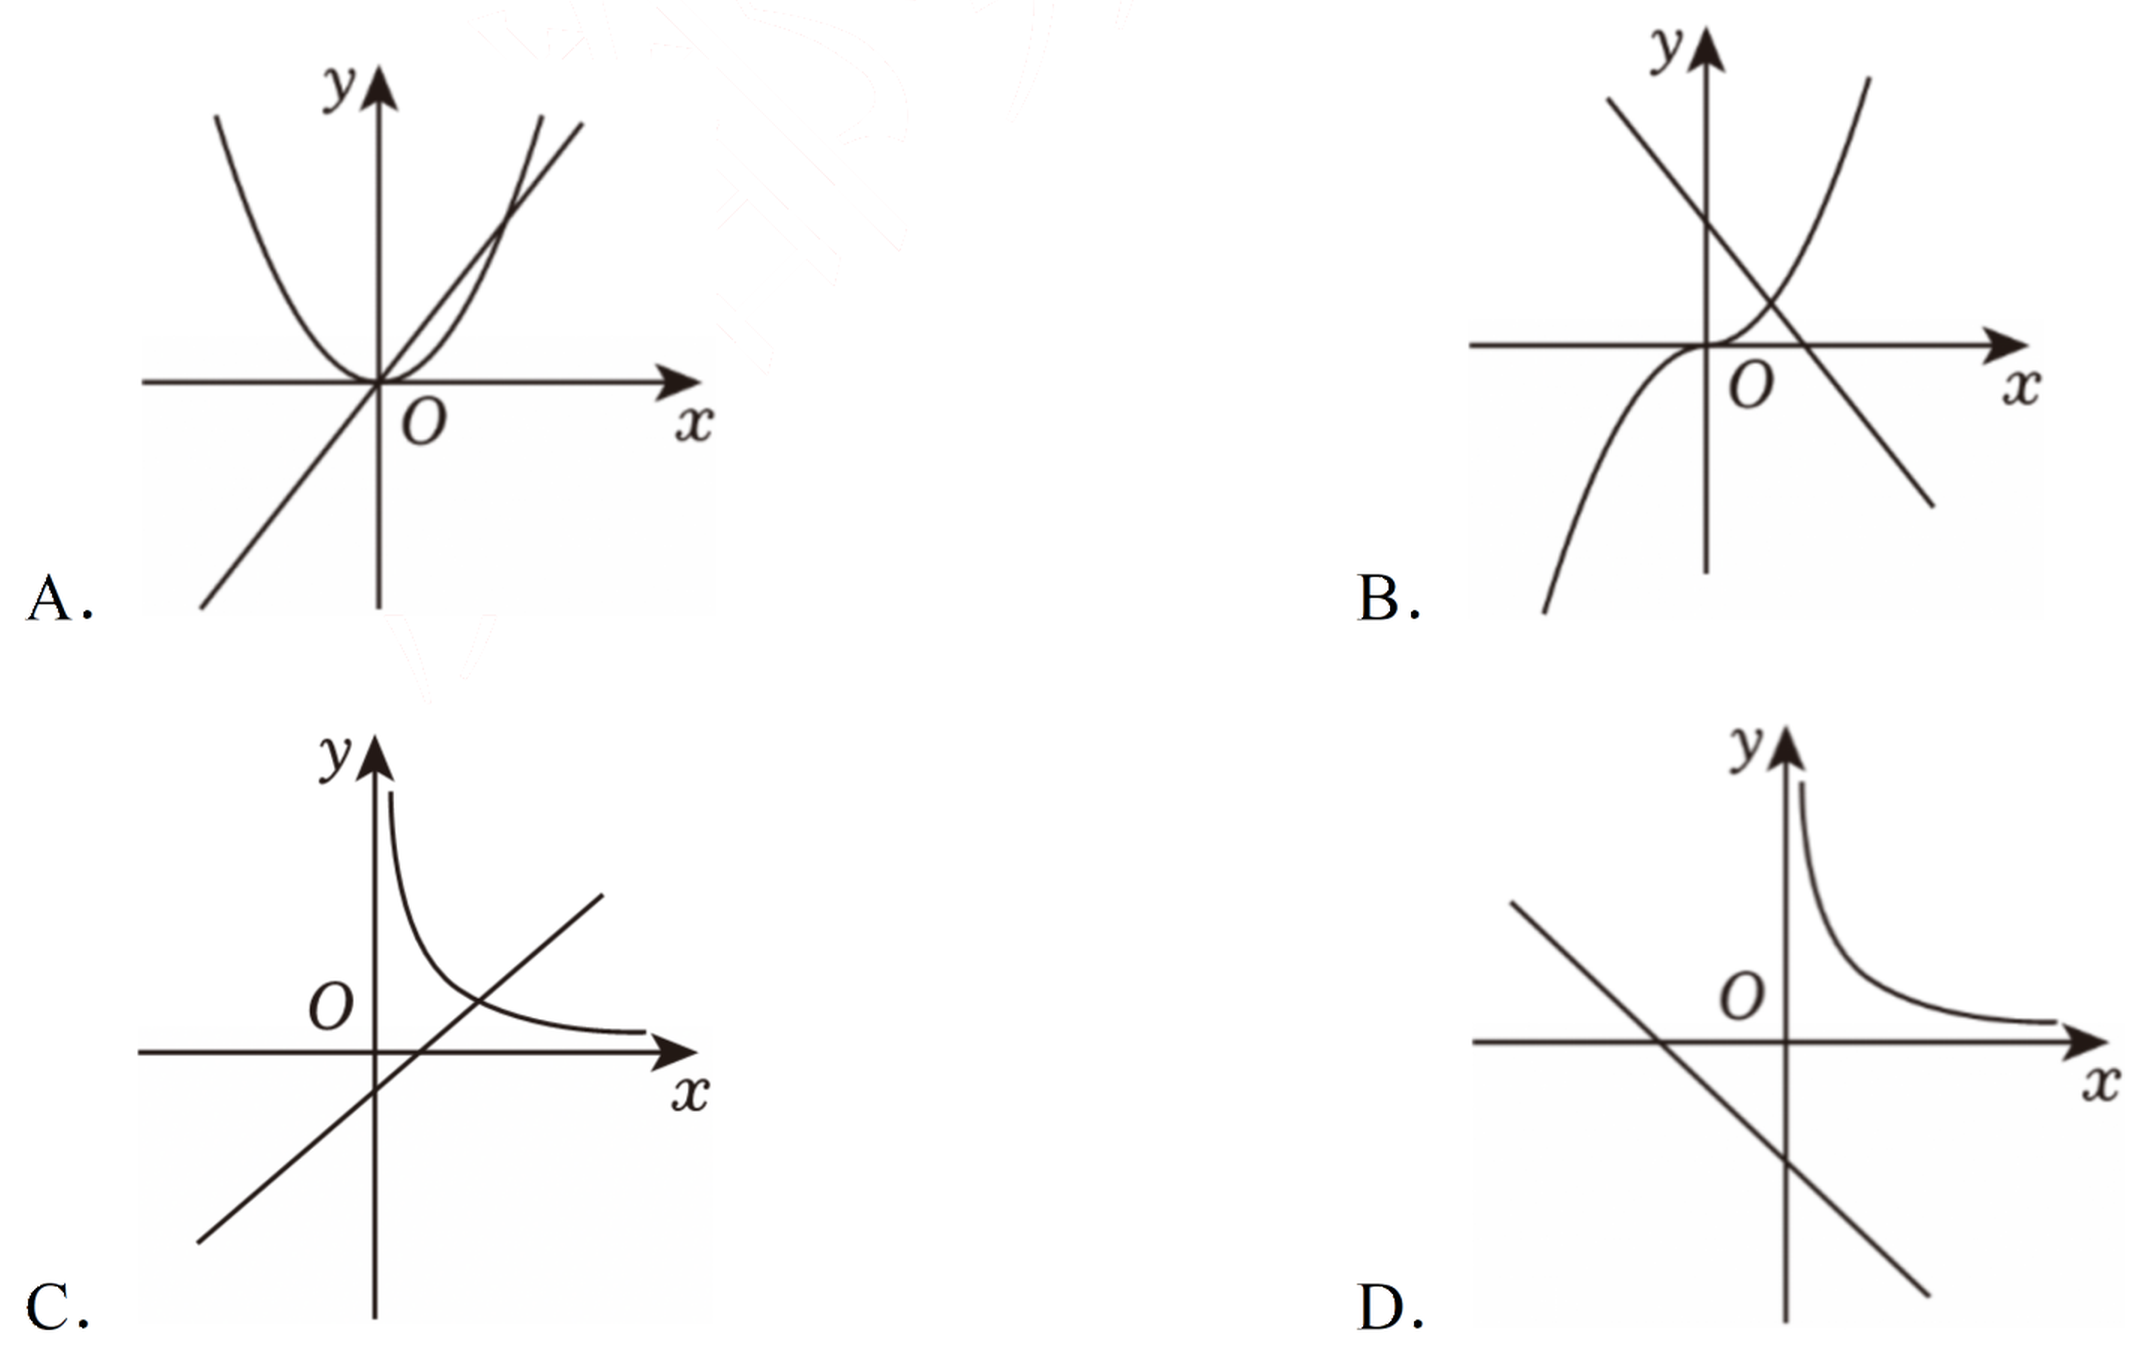
\includegraphics[width=0.80\textwidth]{figures/gao132_q14.png}
\end{center}

\ifanswer
\solbegin
\step{当 $a>0$ 时，$y=ax-\dfrac1a$ 严格增，当 $a<0$ 时，$y=ax-\dfrac1a$ 严格减，}
\step{对于 $A$，因为 $a\ne0$，所以直线 $y=ax-\dfrac1a$ 不过原点，故 $A$ 错误；}
\step{对于 $B$，由函数 $y=x^a(a\ne0)$ 的图象得 $a>1$，}
\step{由 $y=ax-\dfrac1a$ 的图象得 $a<0$，互相矛盾，故 $B$ 错误；}
\step{对于 $C$，由函数 $y=x^a(a\ne0)$ 的图象得 $a>1$，}
\step{由 $y=ax-\dfrac1a$ 的图象得 $a>0$ 且 $-\dfrac1a<0$，符合题意，故 $C$ 正确；}
\step{对于 $D$，由函数 $y=x^a(a\ne0)$ 的图象得 $a<0$，}
\step{由 $y=ax-\dfrac1a$ 的图象得 $a<0$ 且 $-\dfrac1a<0$，互相矛盾，故 $D$ 错误；}
\step{故选 $C$.}
\solend
\fi

\item 中国的 $5G$ 技术领先世界，在 $5G$ 技术中，最大数据传输速率 $C$ 取决于信道带宽 $W$，$C$ 与 $W$ 满足 $C=W\log_2\left(1+\dfrac SN\right)$，其中 $\dfrac SN$ 称为信噪比（单位：$dB$）. 若不改变带宽 $W$，初始信噪比 $\dfrac SN$ 为 $1000$，那么为了使 $C$ 增加 $30\%$，需要将信噪比 $\dfrac SN$ 从 $1000$ 提升至大约\mbox{（\quad）}

\keepwithprev
A. $5000$\qquad\qquad B. $6000$\qquad\qquad C. $7000$\qquad\qquad D. $8000$

\ifanswer
\solbegin
\step{由题意得 $\dfrac SN=1000$ 时，$C=W\log_2(1+1000)\approx W\log_2 1000$，}
\step{要使 $C$ 增加 $30\%$，则 $(1+30\%)C=W\log_2\left(1+\dfrac SN\right)$，即 $1.3C\approx W\log_2\dfrac SN$，}
\step{所以 $1.3\approx\log_{1000}\dfrac SN=\dfrac{\lg\frac SN}{\lg1000}$，所以 $\lg\dfrac SN=3.9$，所以 $\dfrac SN=10^{3.9}\approx8000$.}
\step{故选 $D$.}
\solend
\fi

\item 对于 $a\in\R$，设非空集合 $A=\left\{x\mid\dfrac{(x^2-930x+a)(x-52)}{x+a}=0\right\}$，记 $A$ 中的所有元素之和为 $S(a)$，所有元素之积为 $T(a)$，则下列说法中，不正确的是\mbox{（\quad）}

\keepwithprev
A. 存在实数 $a$，使得 $S(a)=930$

B. 存在实数 $a$，使得 $T(a)=517$

C. 不存在实数 $a$，使得 $T(a)=0$

D. 恰存在 $1$ 个实数 $a$，使得 $T(a)=-52$

\ifanswer
\solbegin
\step{由分式值为 $0$，得分子为 $0$ 且分母不为 $0$，}
\step{分子 $(x^2-930x+a)(x-52)=0$ 的根为 $x=52$}
\step{及方程 $x^2-930x+a=0$ 的两根 $x_1$，$x_2$，}
\step{由根与系数的关系得 $x_1+x_2=930$，$x_1\cdot x_2=a$，}
\step{分母限制 $x\ne-a$，需要剔除等于 $-a$ 的根，}
\step{选项 $A$，取 $a=-52$，$x=52$ 为增根舍去，集合 $A=\{x_1,x_2\}$，}
\step{元素之和 $S(a)=930$，故 $A$ 正确；}
\step{选项 $B$，当无增根时，$T(a)=52a$，令 $52a=517$，得 $a=\dfrac{517}{52}$，}
\step{验证无增根，存在这样的 $a$，故 $B$ 正确；}
\step{选项 $C$，若 $T(a)=0$，则 $0\in A$，代入分子得 $a=0$，}
\step{但 $a=0$ 时分母 $x\ne0$，$x=0$ 为增根，$0$ 不能属于集合 $A$，}
\step{故不存在 $a$ 使得 $T(a)=0$，故 $C$ 正确；}
\step{选项 $D$，当无增根时，令 $52a=-52$，得 $a=-1$；}
\step{当 $x=-a$ 是二次方程的根且不等于 $52$ 时，}
\step{令 $52\times(930+a)=-52$，解得 $a=-931$，验证符合条件；}
\step{当 $a=-52$ 时，$x=52$，舍去，}
\step{集合 $A=\{x_1,x_2\}$，$T(a)=a=-52$，得到两个满足条件的 $a$；}
\step{因此存在 $3$ 个满足条件的 $a$，故 $D$ 错误.}
\step{故选 $D$.}
\solend
\fi

\end{enumerate}

\bigsec{三、解答题}

\begin{enumerate}
\setcounter{enumi}{16}

\item 已知全集 $U=\R$，集合 $A=\left\{x\mid\dfrac{x}{x-3}<0\right\}$，$B=\{x\mid(x-a)(x+4-a)<0\}$.

(1) 当 $a=2$ 时，求 $\overline{B}$、$A\cap\overline{B}$；

(2) 若 $A\cap B=A$，求实数 $a$ 的取值范围.

\ifanswer
\solbegin
\step{(1) $\dfrac{x}{x-3}<0$，即 $x(x-3)<0$，解得 $A=\{x\mid0<x<3\}$，}
\step{当 $a=2$ 时，$B=\{x\mid(x-a)(x+4-a)<0\}=\{x\mid-2<x<2\}$，}
\step{则 $\overline{B}=\{x\mid x\leq-2$ 或 $x\geq2\}$，故 $A\cap\overline{B}=\{x\mid2\leq x<3\}$；}
\step{(2) $A\cap B=A$，则 $A\subseteq B$，故 $\begin{cases}a-4\leq0\\a\geq3\end{cases}$，解得 $3\leq a\leq4$，}
\step{故实数 $a$ 的取值范围是 $\{a\mid3\leq a\leq4\}$.}
\solend
\fi

% 第 18 题是"题干 + 图"约 7cm 的一整块，守卫放在 \item 之前
\needvspace{7cm}
\item 如图，$OA$、$OB$ 是两条长度足够长的互相垂直的笔直小路，矩形 $OCPD$ 的顶点 $C$、$D$ 分别在 $OA$、$OB$ 上，且该矩形区域内种满了荷花. 为了让观赏者有更好的观赏体验，现计划经过点 $P$ 修一条小路 $EF$，其中点 $E$ 在小路 $OA$ 上，点 $F$ 在小路 $OB$ 上，并在 $\triangle OEF$ 区域内种满荷花. 已知 $OD=25m$，$OC=40m$，且小路 $EF$ 要完全位于一个以 $O$ 为顶点的，边长为 $100$ m 的正方形内部（包括边界）. 记 $\triangle OEF$ 的面积为 $S$m$^2$.

(1) 设 $EC=x\cdot m$，试用 $x$ 表示 $OF$，并求 $x$ 的取值范围.

(2) 当 $EC$ 的长度为多少时，$S$ 取得最小值？最小值是多少？

\begin{center}
% 图取原卷 07 页截图去粉色水印，3× LANCZOS 放大
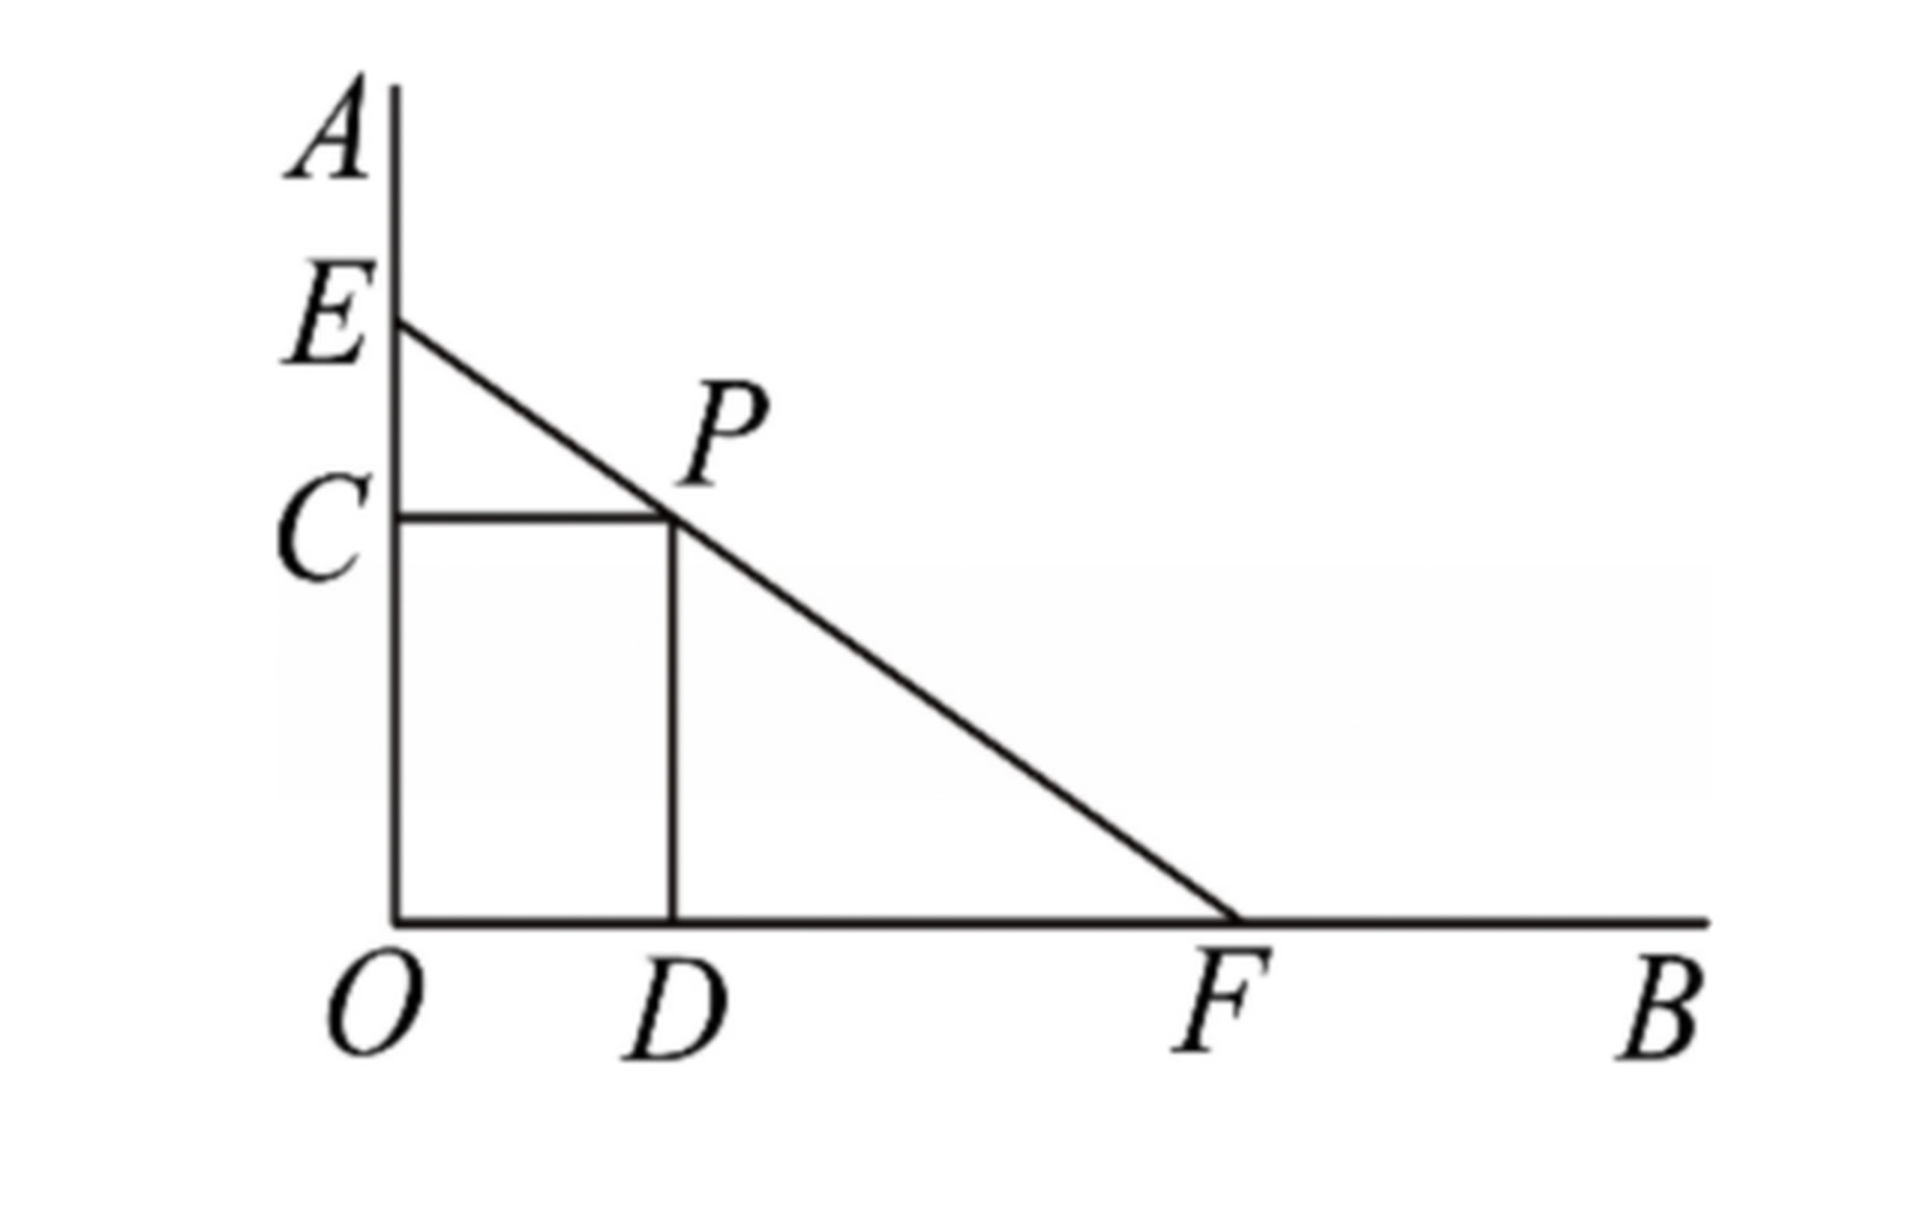
\includegraphics[width=0.32\textwidth]{figures/gao132_q18.png}
\end{center}

\ifanswer
\solbegin
\step{(1) 由题意得 $x\leq60$，}
\step{$\triangle PCE\sim\triangle FDP$，所以 $\dfrac{EC}{CP}=\dfrac{PD}{DF}$，即 $\dfrac{x}{25}=\dfrac{40}{DF}$，得 $DF=\dfrac{1000}{x}$m，}
\step{所以 $OF=OD+DF=\left(25+\dfrac{1000}x\right)$m，}
\step{所以 $25+\dfrac{1000}x\leq100$，解得 $x\geq\dfrac{40}3$；}
\step{综上，$\dfrac{40}3\leq x\leq60$；}
\step{(2) 由 $OE=OC+CE=(40+x)$m，}
\step{所以 $S=\dfrac12 OF\cdot OE=\dfrac12\left(25+\dfrac{1000}x\right)(40+x)$}
\step{$=\dfrac12\left(1000+25x+\dfrac{40000}x+1000\right)$m$^2$，}
\step{由基本不等式得 $S\geq\dfrac12\left(2000+2\sqrt{25x\cdot\dfrac{40000}x}\right)=2000$m$^2$，}
\step{当且仅当 $25x=\dfrac{40000}x$，即 $x=40$ 时取等号，}
\step{故 $EC=40$m 时，$S$ 取得最小值，为 $2000$m$^2$.}
\solend
\fi

\item 已知 $a>0$，$b>0$，请选择适当的方法证明.

(1) 若 $a\ne b$，证明：$a^3+b^3>a^2b+ab^2$；

(2) 若 $ab=1$，证明：$a^2+a<2$ 与 $b^2+b<2$ 不能同时成立.

\ifanswer
\solbegin
\step{(1) 因为 $a>0$，$b>0$，$a\ne b$，}
\step{所以 $a^3+b^3-a^2b-ab^2=a^2(a-b)+b^2(b-a)$}
\step{$=(a^2-b^2)(a-b)=(a-b)^2(a+b)>0$，所以 $a^3+b^3>a^2b+ab^2$.}
\step{(2) 假设 $a^2+a<2$ 与 $b^2+b<2$ 同时成立，所以 $-2<a<1,-2<b<1$，}
\step{又因为 $a>0,b>0$，所以 $0<a<1,0<b<1$，}
\step{所以 $0<ab<1$，这与 $ab=1$ 矛盾，}
\step{故 $a^2+a<2$ 与 $b^2+b<2$ 不可能同时成立.}
\solend
\fi

\item 若设 $M(a,n)=\lvert ax-1\rvert+\lvert ax-2\rvert+\cdots+\lvert ax-n\rvert$ 为曼哈顿扩张距离，它由 $n$ 个绝对值之和组成，其中 $n$ 为正整数.

(1) 若 $M(2,1)\leq5$，求 $x$ 的取值范围；

(2) 若 $k\leq M(2,2)$ 对一切实数 $x$ 恒成立，求实数 $k$ 的取值范围；

(3) $M(2,6)$ 是否存在最小值？若存在，求出该最小值与此时实数 $x$ 的取值范围；若不存在，说明理由.

\ifanswer
\solbegin
\step{(1) $M(2,1)=\lvert2x-1\rvert\leq5$，则不等式可化为 $-5\leq2x-1\leq5$，解得 $-2\leq x\leq3$，}
\step{所以 $x$ 的取值范围为 $[-2,3]$.}
\step{(2) 因为 $k\leq M(2,2)=\lvert2x-1\rvert+\lvert2x-2\rvert$ 对一切实数 $x$ 恒成立，}
\step{又 $\lvert2x-1\rvert+\lvert2x-2\rvert\geq\lvert(2x-1)-(2x-2)\rvert=1$，}
\step{当且仅当 $(2x-1)(2x-2)\leq0$，即 $\dfrac12\leq x\leq1$ 时取等号，}
\step{故 $k\leq1$，所以实数 $k$ 的取值范围为 $(-\infty,1]$.}
\step{(3) $M(2,6)=\lvert2x-1\rvert+\lvert2x-2\rvert+\lvert2x-3\rvert+\lvert2x-4\rvert+\lvert2x-5\rvert+\lvert2x-6\rvert$}
\step{$=2\left(\left\lvert x-\dfrac12\right\rvert+\lvert x-1\rvert+\left\lvert x-\dfrac32\right\rvert+\lvert x-2\rvert+\left\lvert x-\dfrac52\right\rvert+\lvert x-3\rvert\right)$，}
\step{其中 $\left\lvert x-\dfrac12\right\rvert+\lvert x-1\rvert+\left\lvert x-\dfrac32\right\rvert+\lvert x-2\rvert+\left\lvert x-\dfrac52\right\rvert+\lvert x-3\rvert$ 的几何意义为}
\step{在数轴上一点 $x$ 到 $\dfrac12,1,\dfrac32,2,\dfrac52,3$ 的距离之和，}
\step{要想距离之和最小，其中 $x\in\left[\dfrac12,3\right]$ 时，$\left\lvert x-\dfrac12\right\rvert+\lvert x-3\rvert$ 取得最小值，}
\step{当 $x\in\left[1,\dfrac52\right]$ 时，$\lvert x-1\rvert+\left\lvert x-\dfrac52\right\rvert$ 取得最小值，}
\step{当 $x\in\left[\dfrac32,2\right]$ 时，$\left\lvert x-\dfrac32\right\rvert+\lvert x-2\rvert$ 取得最小值，}
\step{综上，当 $x\in\left[\dfrac32,2\right]$ 时，$\left\lvert x-\dfrac12\right\rvert+\lvert x-1\rvert+\left\lvert x-\dfrac32\right\rvert+\lvert x-2\rvert+\left\lvert x-\dfrac52\right\rvert+\lvert x-3\rvert$}
\step{取得最小值，最小值为 $3-\dfrac12+\dfrac52-1+2-\dfrac32=\dfrac92$，}
\step{故 $M(2,6)=2\left(\left\lvert x-\dfrac12\right\rvert+\lvert x-1\rvert+\left\lvert x-\dfrac32\right\rvert+\lvert x-2\rvert+\left\lvert x-\dfrac52\right\rvert+\lvert x-3\rvert\right)$ 的}
\step{最小值为 $9$.}
\solend
\fi

\item 已知集合 $A=\{a_1,a_2,\cdots,a_n\}(0\leq a_1<a_2<\cdots<a_n,n\in\N,n\geq3)$ 具有性质 $Q$：对任意 $i,j(1\leq i\leq j\leq n)$，$a_i+a_j$ 与 $a_j-a_i$ 至少有一个属于集合 $A$；

(1) 判断集合 $M=\{0,2,4\}$ 与 $N=\{2,3,4\}$ 是否具有性质 $Q$，并说明理由；

(2) 已知 $A=\{a_1,a_2,a_3\}$ 具有性质 $Q$，当 $a_2=2026$ 时，求集合 $A$；

(3) 已知 $B=\{b_1,b_2,\cdots,b_{2026}\}$ 具有性质 $Q$，求 $\dfrac{b_1+b_2+\cdots+b_{2026}}{b_{2026}}$ 的值；

\ifanswer
\solbegin
\step{(1) 集合 $M=\{0,2,4\}$ 中，}
\step{因为 $0+2\in M,0+4\in M,4-2\in M,0\pm0=0\in M$，}
\step{$2+2=4\in M,2-2=0\in M,4-4=0\in M$，所以集合 $M$ 具有性质 $Q$；}
\step{集合 $N=\{2,3,4\}$ 中，因为 $3+3=6\notin N,3-3=0\notin N$，}
\step{所以集合 $N$ 不具有性质 $Q$.}
\step{(2) 因为 $a_1<a_2<a_3$，且 $A=\{a_1,a_2,a_3\}$ 具有性质 $Q$，}
\step{所以 $a_3+a_3\notin A,a_3-a_3=0\in A$，则 $a_1=0$，}
\step{又因为 $a_2+a_3>a_3$，所以 $a_2+a_3\notin A$，则 $a_3-a_2\in A$，}
\step{由集合的互异性得 $a_3-a_2=a_2$，而 $a_2=2026$，所以 $a_3=4052$，}
\step{故 $A=\{0,2026,4052\}$；}
\step{(3) 先证明一般结论：$A=\{a_1,a_2,\cdots,a_n\}(0\leq a_1<a_2<\cdots<a_n,n\in\N,n\geq3)$}
\step{具有性质 $Q$，则 $a_1+a_2+a_3+\cdots+a_n=\dfrac n2 a_n$.}
\step{因为 $A=\{a_1,a_2,\cdots,a_n\}(0\leq a_1<a_2<\cdots<a_n,n\in\N,n\geq3)$ 具有性质 $Q$，}
\step{所以 $a_n+a_n\notin A$，则 $a_n-a_n=0\in A$，则 $a_1=0$.}
\step{又因为 $0\leq a_1<a_2<\cdots<a_n$，所以 $0\leq a_n-a_n<a_n-a_{n-1}<\cdots<a_n-a_1$，}
\step{又因为 $a_n+a_{n-i}>a_n(i=1,2,\cdots,n-1)$，所以 $a_n+a_{n-i}\notin A$，}
\step{则 $a_n-a_{n-i}\in A$，}
\step{所以 $a_1=a_n-a_n,a_2=a_n-a_{n-1},a_3=a_n-a_{n-2},\cdots,a_n=a_n-a_1$.}
\step{所以 $a_1+a_2+a_3+\cdots+a_n$}
\step{$=(a_n-a_n)+(a_n-a_{n-1})+(a_n-a_{n-2})+\cdots+(a_n-a_1)$，}
\step{即 $a_1+a_2+a_3+\cdots+a_n=\dfrac n2 a_n$，}
\step{所以 $B=\{b_1,b_2,\cdots,b_{2026}\}$ 具有性质 $Q$，则 $b_1+b_2+\cdots+b_{2026}=\dfrac{2026}{2}b_{2026}$，}
\step{所以 $\dfrac{b_1+b_2+\cdots+b_{2026}}{b_{2026}}=\dfrac{2026}{2}=1013$.}
\solend
\fi

\end{enumerate}

% 行数复核：逐题数 \step 条数，合计 144 条（Q3：4；Q4：1；Q5：4；Q6：2；Q7：9；Q8：2；
% Q9：3；Q10：6；Q11：9；Q12：9；Q13：0；Q14：9；Q15：4；Q16：19；Q17：5；Q18：11；
% Q19：7；Q20：17；Q21：23），与原卷印刷行逐题相等（cases 块作一个印刷行计）。
% 第 13 题只印括号内答案、提 \ans{}，不计入 \step 账；第 14—16 题答案在解析末句，
% 括号内留空、不另提 \ans{}。

\end{document}
"
%
% 原始材料：微信公众号"魔都数学加油站"文章，作者破晓，2026-11-14 19:00 发布；
% 连载"27学年高一132"，原文标题"27学年高一132——2026-2027年上海市川沙中学高一上期中"；
% 原文链接：https://mp.weixin.qq.com/s/VBG01CrUNMIYWWHhSfz8JQ。
% 正文为 11 张 PNG 页（01、04、06、07、09、11 为 2560x3620，02、03、05、08、10 为 4762x6735），
% 题目下印有【解析】，为讲评版。题目、解析均据原图转录；
% 卷面粉红色水印"魔都数学加油站"及公众号页脚未录入。全卷 2 幅插图：第 14 题四幅坐标图选项、
% 第 18 题矩形 OCPD 与小路 EF 示意图，均取原卷 04／07 页截图去水印。
%
% 卷首标题：原卷印作"2026-2027 年川沙中学高一上期中"（公众号标题中的"上海市"
% 卷面标题行没有，本稿照卷面），年份区间按全稿惯例排 en dash；原卷未印副标题，
% 本卷为期中卷、跨集合与常用逻辑用语／不等式／函数三章，按题目内容标为
% "集合与常用逻辑用语、不等式、函数"（与 125／126／128／129／131 同期中卷口径相同）：
% 集合与逻辑见 Q5、Q6、Q17、Q21，不等式见 Q3、Q4、Q9、Q10、Q12、Q13、Q15、Q16、Q19，
% 函数（幂函数、指数／对数、基本不等式应用）见 Q7、Q8、Q11、Q14、Q18、Q20。
%
% 题号体例：本卷共 19 题——一、填空题 3—12（10 题）、二、选择题 13—16（4 题）、
% 三、解答题 17—21（5 题）。三节分别 \setcounter{enumi}{2}／{12}／{16}。
%
% 与原卷的排版差异：
%   ① 原文从第 3 题起，本稿保留原题号（见上"题号体例"）；
%   ② 原卷每题下直接印【解析】，本稿按全稿惯例置于答案版；第 13 题答案 D 印在题干
%      括号内、无独立答案段，按 高一37／52／53／55／63／64／128／131 成例括号留空、
%      另提 \ans{$D$}；第 14—16 题答案在解析末句"故选 …"，括号内留空、不另提 \ans{}；
%   ③ 原卷未印副标题，本稿按"知识模块"口径补出；
%   ④ 原卷填空横线按全稿惯例排为 \blankline[4.4em]；选择题括号排 \mbox{（\quad）}、
%      选项段前按惯例加 \keepwithprev；解答题不留作答区（原卷为讲评版，与 109—131 同）；
%   ⑤ 原卷数集排斜体 $R^+$／$R$／$Z$／$N$，按全稿惯例改 \R^+／\R／\Z／\N；
%      绝对值排 \lvert…\rvert，集合描述竖线排 \mid；不等号按全稿惯例排 \leqslant／\geqslant；
%      补集照原卷上划线排 \overline{B}；
%   ⑥ 子题标号 (1)(2)(3) 原卷用半角括号，照录；第 14 题四幅坐标图选项按原卷 2×2 排布
%      合并裁为一张 \includegraphics（未用 TikZ 重绘，以保证与原卷一致），题前加
%      \needvspace{9cm} 守卫；第 18 题图取 07 页截图，题前按惯例加 \needvspace{7cm} 守卫
%      （照 高一120／127／129／131 成例），两者守卫都放在 \item 之前；
%   ⑦ 原卷 Q7 解析跨 01—02 页、Q10 解析跨 02—03 页、Q12 解析跨 03—04 页、
%      Q14 解析跨 04—05 页、Q16 解析在 06 页、Q18 解析跨 07—08 页、
%      Q20 解析跨 08—09 页、Q21 解析跨 10—11 页，本稿按题合并连续排版；
%      末页第 11 页为 Q21 (3) 解析的续尾，按实际印刷行单列。
%
% 判别式字形：第 10 题 $\triangle=4(a-1)^2+16(a-1)<0$、第 11 题
%   $\triangle=4(m-2)^2-4(m^2-3m+3)=-4m+4>0$ 两处原卷均排 $\triangle$（等边、扁），
%   逐处放大核对、字形一致，照录 \triangle；与 高一129／131 同题排 $\Delta$（等腰、高）不同。
%   全卷 \triangle 兼作第 18 题「$\triangle PCE\sim\triangle FDP$」「$\triangle OEF$」的几何
%   三角形记号，全卷未出现 \Delta。
%
% 子集符号：第 5 题解析 $B\subseteq A$、第 17 题 (2) 解析 $A\subseteq B$ 均印带下划线，
%   照录 \subseteq；全卷未出现单线 \subset。
%
% 原卷存疑照录：
%   第 9 题题干作"充分非必要条件"、解析作"充分不必要条件"，措辞不同，照录；
%   第 10 题解析"当 $a-1=0$ 时，$-4\geq0$，不等式不成立，$a=1$ 满足题意"照录；
%   第 11 题解析"所以 $2(m-1)+\dfrac1{m-1}\leq-2\sqrt2$"由上一行 $2(1-m)+\dfrac1{1-m}\geq2\sqrt2$
%     直接变号得到，照录；
%   第 12 题解析"由 $x\in Z$，$-7<-2\sqrt{10}<-6$"与"即 $k^2+7k+10\leq0$，解得 $-5\leq k\leq-2$"照录；
%   第 16 题解析"令 $52\times(930+a)=-52$，解得 $a=-931$"（按式应为 $a=-931$ 之外的解）照录；
%   第 19 题 (2) 解析"所以 $-2<a<1,-2<b<1$"数学式内半角逗号，照录；
%   第 20 题 (3) 解析"最小值为 $3-\dfrac12+\dfrac52-1+2-\dfrac32=\dfrac92$"与
%     "故 $M(2,6)=\dots$ 的最小值为 9"两处结论并列，照录；
%   第 21 题 (1) 解析"$0+2\in M,0+4\in M,4-2\in M,0\pm0=0\in M$"、
%     "$2+2=4\in M,2-2=0\in M,4-4=0\in M$"、(3) 各连写等式内半角逗号，照录；
%   第 21 题 (3) 解析"即 $a_1+a_2+a_3+\cdots+a_n=\dfrac n2 a_n$，"句末用半角逗号，照录。
%
% 行数复核：见文末"行数复核"注（逐题 \step 条数与原卷印刷行逐题相等，cases 块作一个印刷行计）。
%   第 13 题只印括号内答案、提 \ans{}，不计入 \step 账；第 14—16 题答案在解析末句，
%   括号内留空、不另提 \ans{}。
%
\documentclass[a4paper,11pt]{article}
\usepackage{common}

\begin{document}

\examtitlest[3]{2026--2027 年川沙中学高一上期中}{集合与常用逻辑用语、不等式、函数}

\bigsec{一、填空题}

\begin{enumerate}
\setcounter{enumi}{2}

\item 已知 $a$、$b\in\R^+$ 且 $ab=2$，则 $a+2b$ 的最小值为\blankline[4.4em].

\ifanswer
\solbegin
\step{因为 $a\in\R^+$，$b\in\R^+$ 且 $ab=2$，}
\step{由基本不等式得 $a+2b\geq2\sqrt{a\cdot2b}=2\sqrt{2ab}=2\sqrt4=4$.}
\step{等号当且仅当 $a=2b$ 时成立，结合 $ab=2$ 解得 $b=1$，$a=2$，}
\step{所以 $a+2b$ 的最小值为 $4$.}
\solend
\fi

\item 如果幂函数 $f(x)=(m^2-3m-3)x^{m^2+m-3}$ 在 $(0,+\infty)$ 上是增函数，则实数 $m=$\blankline[4.4em].

\ifanswer
\solbegin
\step{由已知得 $\begin{cases}m^2-3m-3=1\\m^2+m-3>0\end{cases}$，所以 $m=4$.}
\solend
\fi

\item 已知集合 $A=\{1,2\}$，集合 $B=\{x\mid ax=6\}$，若 $A\cup B=A$，则 $a$ 的所有取值构成的集合为\blankline[4.4em].

\ifanswer
\solbegin
\step{因为 $A\cup B=A$，所以 $B\subseteq A$，}
\step{当 $a=0$ 时，$B=\varnothing$，满足 $B\subseteq A$；}
\step{当 $a\ne0$ 时，$B=\left\{\dfrac6a\right\}$，则 $\dfrac6a=1$ 或 $\dfrac6a=2$，解得 $a=6$ 或 $a=3$，}
\step{综上所述，$a$ 的所有取值构成的集合为 $\{0,3,6\}$.}
\solend
\fi

\item 设全集为 $\R$，$A=\{y\mid y=-x^2+2x+1\}$，$B=\{x\mid y=\ln(x-1)\}$，则 $A\cap B=$\blankline[4.4em].

\ifanswer
\solbegin
\step{$A=\{y\mid y=-x^2+2x+1\}=\{y\mid y=-(x-1)^2+2\}=\{y\mid y\leq2\}$，}
\step{$B=\{x\mid y=\ln(x-1)\}=\{x\mid x>1\}$，则 $A\cap B=(1,2]$.}
\solend
\fi

\item 已知 $x\in\R$，则方程 $\lvert 6-x\rvert+\lvert 6x-3\rvert=\lvert 5x+3\rvert$ 的解集为\blankline[4.4em].

\ifanswer
\solbegin
\step{当 $x<-\dfrac35$ 时，$6-x>0$，$6x-3<0$，$5x+3<0$，}
\step{原方程为 $6-x-6x+3=-5x-3$，解得 $x=6$，不满足 $x<-\dfrac35$；}
\step{当 $-\dfrac35\leq x\leq\dfrac12$ 时，$5x+3\geq0$，$6x-3<0$，$6-x>0$，}
\step{原方程为 $6-x+3-6x=5x+3$，解得 $x=\dfrac12$；}
\step{当 $\dfrac12<x\leq6$ 时，$5x+3>0$，$6x-3>0$，$6-x\geq0$，}
\step{原方程为 $6-x+6x-3=5x+3$，即 $0=0$，恒成立，所以 $\dfrac12<x\leq6$；}
\step{当 $x>6$ 时，$5x+3\geq0$，$6x-3>0$，$6-x<0$，}
\step{原方程为 $x-6+6x-3=5x+3$，解得 $x=6$，不满足 $x>6$；}
\step{综上 $\dfrac12\leq x\leq6$，所以原方程的解集为 $\left\{x\mid\dfrac12\leq x\leq6\right\}$.}
\solend
\fi

\item 已知 $\log_2 3=a,2^b=7$，用 $a,b$ 表示 $\log_{42}56$ 为\blankline[4.4em].

\ifanswer
\solbegin
\step{$\log_{42}56=\dfrac{\log_2 56}{\log_2 42}=\dfrac{\log_2(7\times8)}{\log_2(6\times7)}=\dfrac{\log_2 7+\log_2 8}{\log_2 6+\log_2 7}$}
\step{$=\dfrac{\log_2 7+\log_2 2^3}{\log_2 2+\log_2 3+\log_2 7}=\dfrac{b+3}{1+a+b}$.}
\solend
\fi

\item 已知 $\dfrac13<x<\dfrac12$ 是不等式 $\lvert x-m\rvert<1$ 成立的充分非必要条件，则 $m$ 的取值范围是\blankline[4.4em].

\ifanswer
\solbegin
\step{因为 $\lvert x-m\rvert<1$，所以 $-1<x-m<1$，所以 $m-1<x<m+1$，}
\step{所以 $m-1<x<m+1$ 成立的充分不必要条件是 $\dfrac13<x<\dfrac12$，}
\step{所以 $\begin{cases}m-1\leq\dfrac13\\m+1\geq\dfrac12\end{cases}$，解得 $-\dfrac12\leq m\leq\dfrac43$，故 $m$ 的取值范围是 $\left[-\dfrac12,\dfrac43\right]$.}
\solend
\fi

\item 若关于 $x$ 的不等式 $(a-1)x^2+2(a-1)x-4\geq0$ 的解集为空集，则 $a$ 的取值范围是\blankline[4.4em].

\ifanswer
\solbegin
\step{关于 $x$ 的不等式 $(a-1)x^2+2(a-1)x-4\geq0$ 的解集为 $\varnothing$，}
\step{当 $a-1=0$ 时，$-4\geq0$，不等式不成立，$a=1$ 满足题意；}
\step{当 $a-1>0$ 时，$a>1$，不等式的解集不为空集，不满足题意；}
\step{当 $a-1<0$ 时，$a<1$，当 $\triangle=4(a-1)^2+16(a-1)<0$ 时，即 $(a-1)(a+3)<0$，}
\step{解得 $-3<a<1$，满足题意；}
\step{综上，实数 $a$ 的取值范围是 $\{a\mid-3<a\leq1\}$.}
\solend
\fi

\item 已知关于 $x$ 的方程 $x^2+2(m-2)x+m^2-3m+3=0$ 有两个不相等的实数根 $x_1$、$x_2$，则 $\dfrac{mx_1}{x_1-1}+\dfrac{mx_2}{x_2-1}-\dfrac{2}{x_1+x_2-2}$ 的最大值为\blankline[4.4em].

\ifanswer
\solbegin
\step{关于 $x$ 的方程 $x^2+2(m-2)x+m^2-3m+3=0$ 有两个不相等的实数根 $x_1$、$x_2$，}
\step{则 $\triangle=4(m-2)^2-4(m^2-3m+3)=-4m+4>0$，得 $m<1$，}
\step{且 $x_1+x_2=-2(m-2)$，$x_1x_2=m^2-3m+3$，}
\step{$\dfrac{mx_1}{x_1-1}+\dfrac{mx_2}{x_2-1}-\dfrac{2}{x_1+x_2-2}=\dfrac{m[2x_1x_2-(x_1+x_2)]}{x_1x_2-(x_1+x_2)+1}+\dfrac1{m-1}$}
\step{$=\dfrac{2m(m-1)^2}{m^2-m}+\dfrac1{m-1}=2(m-1)+\dfrac1{m-1}$，}
\step{又因为 $m<1$，所以 $m-1<0$，则 $1-m>0$，}
\step{所以 $2(1-m)+\dfrac1{1-m}\geq2\sqrt{2(1-m)\cdot\dfrac1{1-m}}=2\sqrt2$，}
\step{当且仅当 $2(1-m)=\dfrac1{1-m}$ 时，即 $m=1-\dfrac{\sqrt2}2$ 时取等号，}
\step{所以 $2(m-1)+\dfrac1{m-1}\leq-2\sqrt2$，即 $\dfrac{mx_1}{x_1-1}+\dfrac{mx_2}{x_2-1}-\dfrac2{x_1+x_2-2}$ 的最大值为 $-2\sqrt2$.}
\solend
\fi

\item 若使集合 $A=\{x\mid(kx-k^2-10)(x-1)>0,x\in\Z\}$ 中的元素个数最少，则实数 $k$ 的取值范围是\blankline[4.4em].

\ifanswer
\solbegin
\step{由题意集合 $A=\{x\mid(kx-k^2-10)(x-1)>0,\ x\in\Z\}$，}
\step{$k=0$ 时，不等式解得 $x<1$，有无数个整数解；}
\step{$k\ne0$ 时，则不等式变形为 $k\left(x-k-\dfrac{10}k\right)(x-1)>0$，}
\step{当 $k>0$ 时，$k+\dfrac{10}k\geq2\sqrt{10}$，仅当 $k=\sqrt{10}$ 时等号成立，}
\step{此时不等式解得 $x>k+\dfrac{10}k$ 或 $x<1$，有无数个整数解；}
\step{当 $k<0$ 时，$k+\dfrac{10}k=-\left[(-k)+\left(-\dfrac{10}k\right)\right]\leq-2\sqrt{10}$，仅当 $k=-\sqrt{10}$ 时等号成立，}
\step{此时不等式解得 $k+\dfrac{10}k<x<1$，}
\step{由 $x\in\Z$，$-7<-2\sqrt{10}<-6$，要使集合 $A$ 中的元素最少，则 $k+\dfrac{10}k\geq-7$，}
\step{即 $k^2+7k+10\leq0$，解得 $-5\leq k\leq-2$，故实数 $k$ 的取值范围是 $[-5,-2]$.}
\solend
\fi

\end{enumerate}

\bigsec{二、选择题}

\begin{enumerate}
\setcounter{enumi}{12}

\item 下列说法正确的是\mbox{（\quad）}

\keepwithprev
A. 若 $a>b$，则 $\dfrac1a<\dfrac1b$\qquad\qquad B. 若 $a>b$，$c>d$，则 $ac>bd$

C. 若 $a>b$，则 $ac^2>bc^2$\qquad\qquad D. 若 $ac^2>bc^2$，则 $a>b$

\ifanswer
\ans{$D$}
\fi

% 第 14 题四幅坐标图选项是一整块，守卫放在 \item 之前
\needvspace{9cm}
\item 在同一坐标系内，函数 $y=x^a(a\ne0)$ 和 $y=ax-\dfrac1a$ 的图象可能是\mbox{（\quad）}

\keepwithprev
\begin{center}
% 四幅坐标图选项取原卷 04 页截图去粉色水印，按原卷 2×2 排布合并为一张
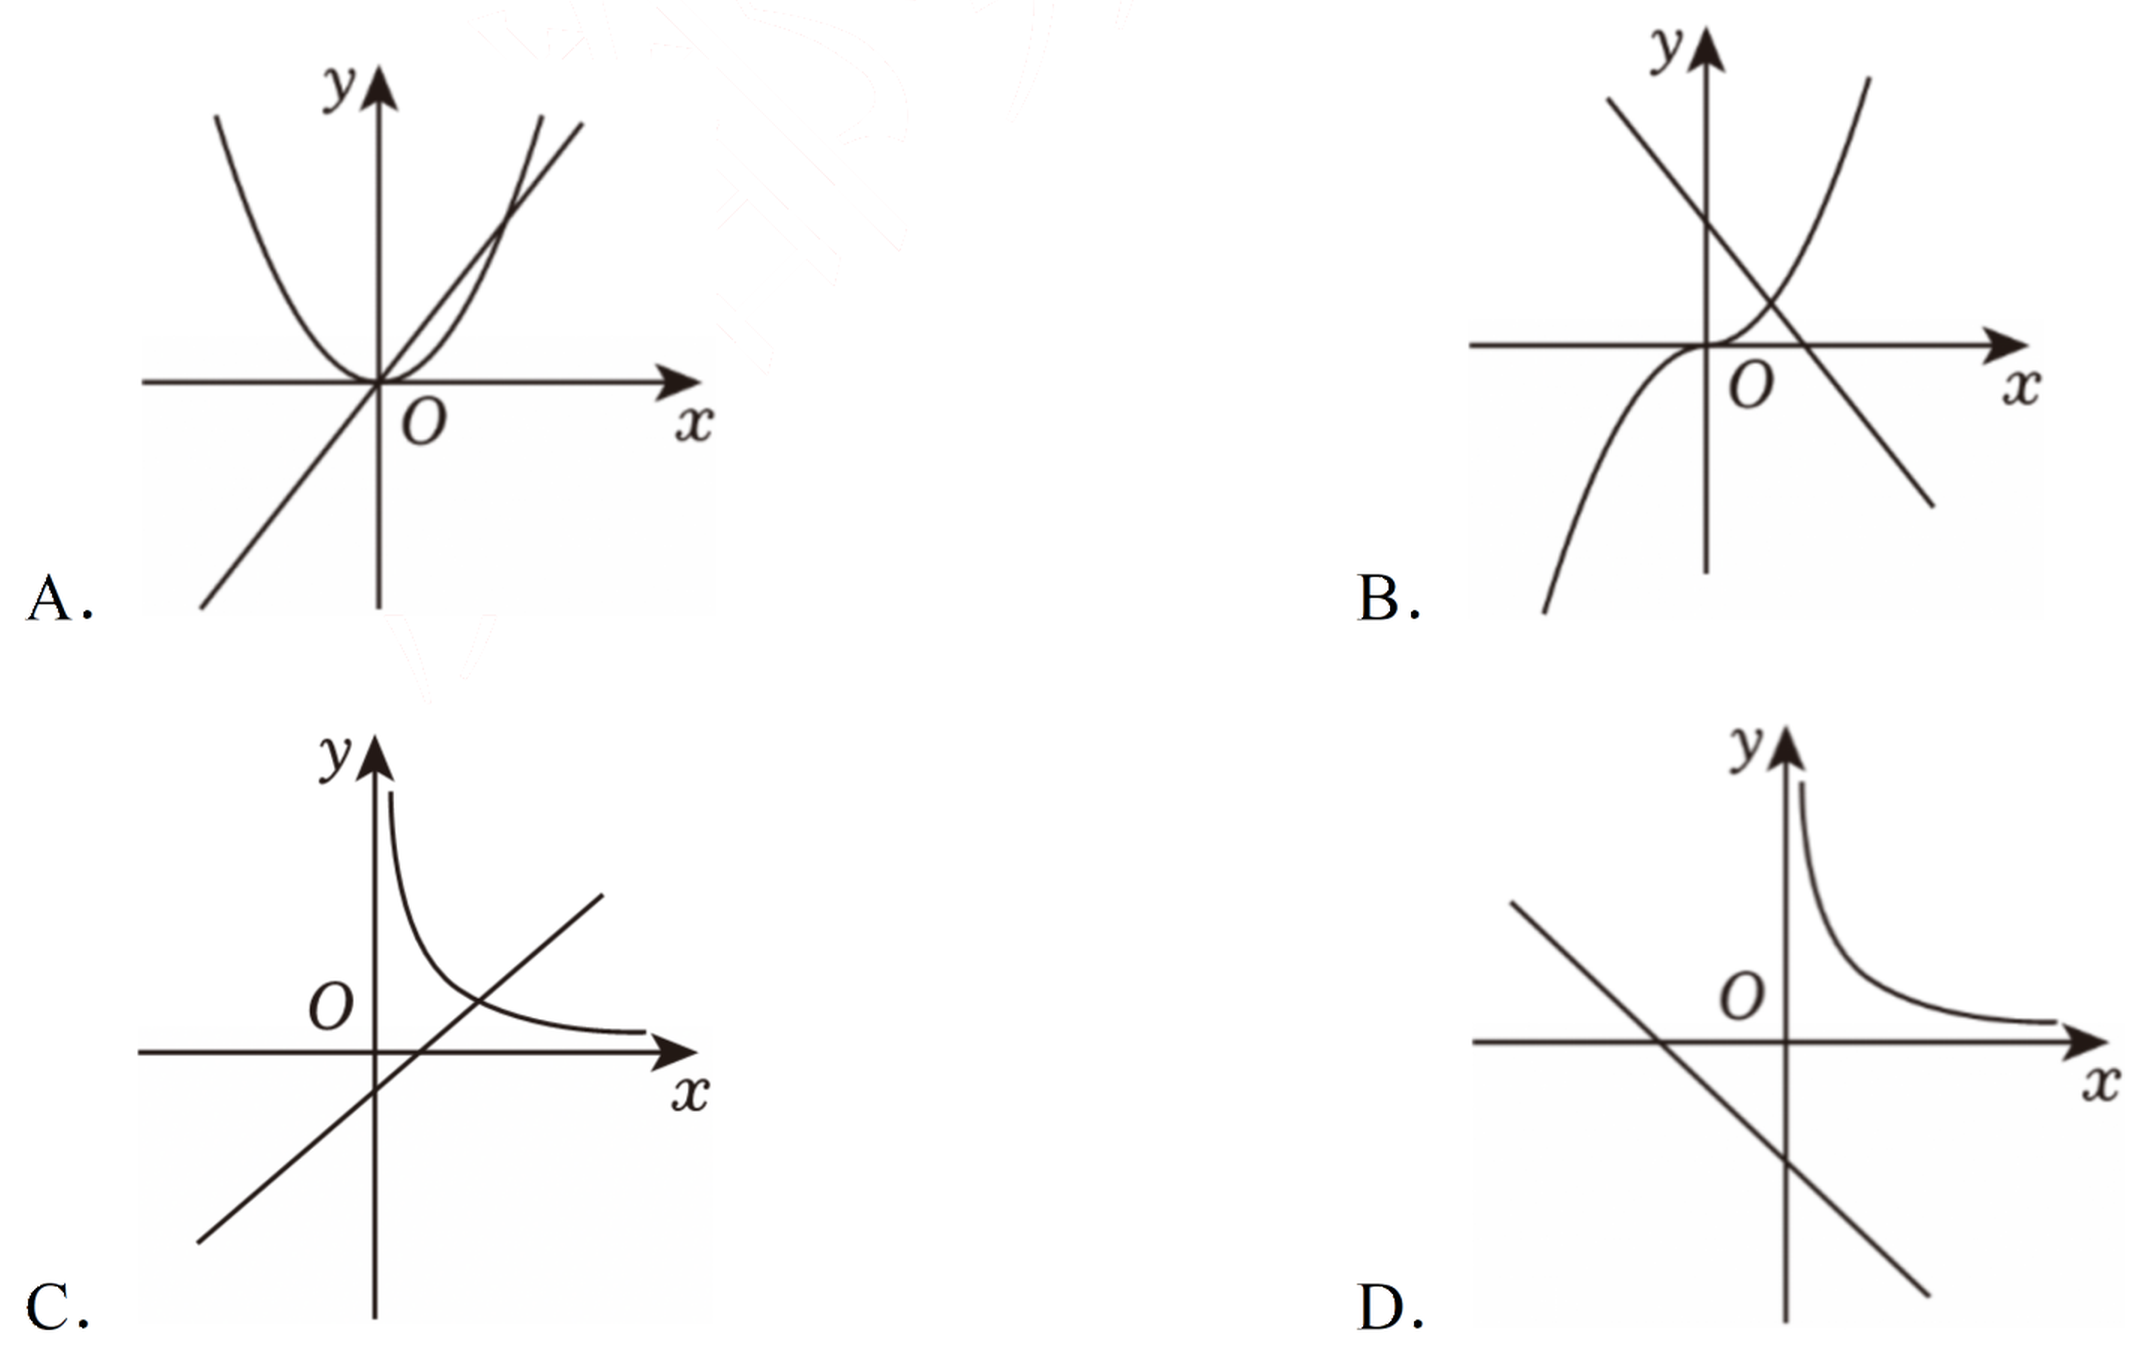
\includegraphics[width=0.80\textwidth]{figures/gao132_q14.png}
\end{center}

\ifanswer
\solbegin
\step{当 $a>0$ 时，$y=ax-\dfrac1a$ 严格增，当 $a<0$ 时，$y=ax-\dfrac1a$ 严格减，}
\step{对于 $A$，因为 $a\ne0$，所以直线 $y=ax-\dfrac1a$ 不过原点，故 $A$ 错误；}
\step{对于 $B$，由函数 $y=x^a(a\ne0)$ 的图象得 $a>1$，}
\step{由 $y=ax-\dfrac1a$ 的图象得 $a<0$，互相矛盾，故 $B$ 错误；}
\step{对于 $C$，由函数 $y=x^a(a\ne0)$ 的图象得 $a>1$，}
\step{由 $y=ax-\dfrac1a$ 的图象得 $a>0$ 且 $-\dfrac1a<0$，符合题意，故 $C$ 正确；}
\step{对于 $D$，由函数 $y=x^a(a\ne0)$ 的图象得 $a<0$，}
\step{由 $y=ax-\dfrac1a$ 的图象得 $a<0$ 且 $-\dfrac1a<0$，互相矛盾，故 $D$ 错误；}
\step{故选 $C$.}
\solend
\fi

\item 中国的 $5G$ 技术领先世界，在 $5G$ 技术中，最大数据传输速率 $C$ 取决于信道带宽 $W$，$C$ 与 $W$ 满足 $C=W\log_2\left(1+\dfrac SN\right)$，其中 $\dfrac SN$ 称为信噪比（单位：$dB$）. 若不改变带宽 $W$，初始信噪比 $\dfrac SN$ 为 $1000$，那么为了使 $C$ 增加 $30\%$，需要将信噪比 $\dfrac SN$ 从 $1000$ 提升至大约\mbox{（\quad）}

\keepwithprev
A. $5000$\qquad\qquad B. $6000$\qquad\qquad C. $7000$\qquad\qquad D. $8000$

\ifanswer
\solbegin
\step{由题意得 $\dfrac SN=1000$ 时，$C=W\log_2(1+1000)\approx W\log_2 1000$，}
\step{要使 $C$ 增加 $30\%$，则 $(1+30\%)C=W\log_2\left(1+\dfrac SN\right)$，即 $1.3C\approx W\log_2\dfrac SN$，}
\step{所以 $1.3\approx\log_{1000}\dfrac SN=\dfrac{\lg\frac SN}{\lg1000}$，所以 $\lg\dfrac SN=3.9$，所以 $\dfrac SN=10^{3.9}\approx8000$.}
\step{故选 $D$.}
\solend
\fi

\item 对于 $a\in\R$，设非空集合 $A=\left\{x\mid\dfrac{(x^2-930x+a)(x-52)}{x+a}=0\right\}$，记 $A$ 中的所有元素之和为 $S(a)$，所有元素之积为 $T(a)$，则下列说法中，不正确的是\mbox{（\quad）}

\keepwithprev
A. 存在实数 $a$，使得 $S(a)=930$

B. 存在实数 $a$，使得 $T(a)=517$

C. 不存在实数 $a$，使得 $T(a)=0$

D. 恰存在 $1$ 个实数 $a$，使得 $T(a)=-52$

\ifanswer
\solbegin
\step{由分式值为 $0$，得分子为 $0$ 且分母不为 $0$，}
\step{分子 $(x^2-930x+a)(x-52)=0$ 的根为 $x=52$}
\step{及方程 $x^2-930x+a=0$ 的两根 $x_1$，$x_2$，}
\step{由根与系数的关系得 $x_1+x_2=930$，$x_1\cdot x_2=a$，}
\step{分母限制 $x\ne-a$，需要剔除等于 $-a$ 的根，}
\step{选项 $A$，取 $a=-52$，$x=52$ 为增根舍去，集合 $A=\{x_1,x_2\}$，}
\step{元素之和 $S(a)=930$，故 $A$ 正确；}
\step{选项 $B$，当无增根时，$T(a)=52a$，令 $52a=517$，得 $a=\dfrac{517}{52}$，}
\step{验证无增根，存在这样的 $a$，故 $B$ 正确；}
\step{选项 $C$，若 $T(a)=0$，则 $0\in A$，代入分子得 $a=0$，}
\step{但 $a=0$ 时分母 $x\ne0$，$x=0$ 为增根，$0$ 不能属于集合 $A$，}
\step{故不存在 $a$ 使得 $T(a)=0$，故 $C$ 正确；}
\step{选项 $D$，当无增根时，令 $52a=-52$，得 $a=-1$；}
\step{当 $x=-a$ 是二次方程的根且不等于 $52$ 时，}
\step{令 $52\times(930+a)=-52$，解得 $a=-931$，验证符合条件；}
\step{当 $a=-52$ 时，$x=52$，舍去，}
\step{集合 $A=\{x_1,x_2\}$，$T(a)=a=-52$，得到两个满足条件的 $a$；}
\step{因此存在 $3$ 个满足条件的 $a$，故 $D$ 错误.}
\step{故选 $D$.}
\solend
\fi

\end{enumerate}

\bigsec{三、解答题}

\begin{enumerate}
\setcounter{enumi}{16}

\item 已知全集 $U=\R$，集合 $A=\left\{x\mid\dfrac{x}{x-3}<0\right\}$，$B=\{x\mid(x-a)(x+4-a)<0\}$.

(1) 当 $a=2$ 时，求 $\overline{B}$、$A\cap\overline{B}$；

(2) 若 $A\cap B=A$，求实数 $a$ 的取值范围.

\ifanswer
\solbegin
\step{(1) $\dfrac{x}{x-3}<0$，即 $x(x-3)<0$，解得 $A=\{x\mid0<x<3\}$，}
\step{当 $a=2$ 时，$B=\{x\mid(x-a)(x+4-a)<0\}=\{x\mid-2<x<2\}$，}
\step{则 $\overline{B}=\{x\mid x\leq-2$ 或 $x\geq2\}$，故 $A\cap\overline{B}=\{x\mid2\leq x<3\}$；}
\step{(2) $A\cap B=A$，则 $A\subseteq B$，故 $\begin{cases}a-4\leq0\\a\geq3\end{cases}$，解得 $3\leq a\leq4$，}
\step{故实数 $a$ 的取值范围是 $\{a\mid3\leq a\leq4\}$.}
\solend
\fi

% 第 18 题是"题干 + 图"约 7cm 的一整块，守卫放在 \item 之前
\needvspace{7cm}
\item 如图，$OA$、$OB$ 是两条长度足够长的互相垂直的笔直小路，矩形 $OCPD$ 的顶点 $C$、$D$ 分别在 $OA$、$OB$ 上，且该矩形区域内种满了荷花. 为了让观赏者有更好的观赏体验，现计划经过点 $P$ 修一条小路 $EF$，其中点 $E$ 在小路 $OA$ 上，点 $F$ 在小路 $OB$ 上，并在 $\triangle OEF$ 区域内种满荷花. 已知 $OD=25m$，$OC=40m$，且小路 $EF$ 要完全位于一个以 $O$ 为顶点的，边长为 $100$ m 的正方形内部（包括边界）. 记 $\triangle OEF$ 的面积为 $S$m$^2$.

(1) 设 $EC=x\cdot m$，试用 $x$ 表示 $OF$，并求 $x$ 的取值范围.

(2) 当 $EC$ 的长度为多少时，$S$ 取得最小值？最小值是多少？

\begin{center}
% 图取原卷 07 页截图去粉色水印，3× LANCZOS 放大
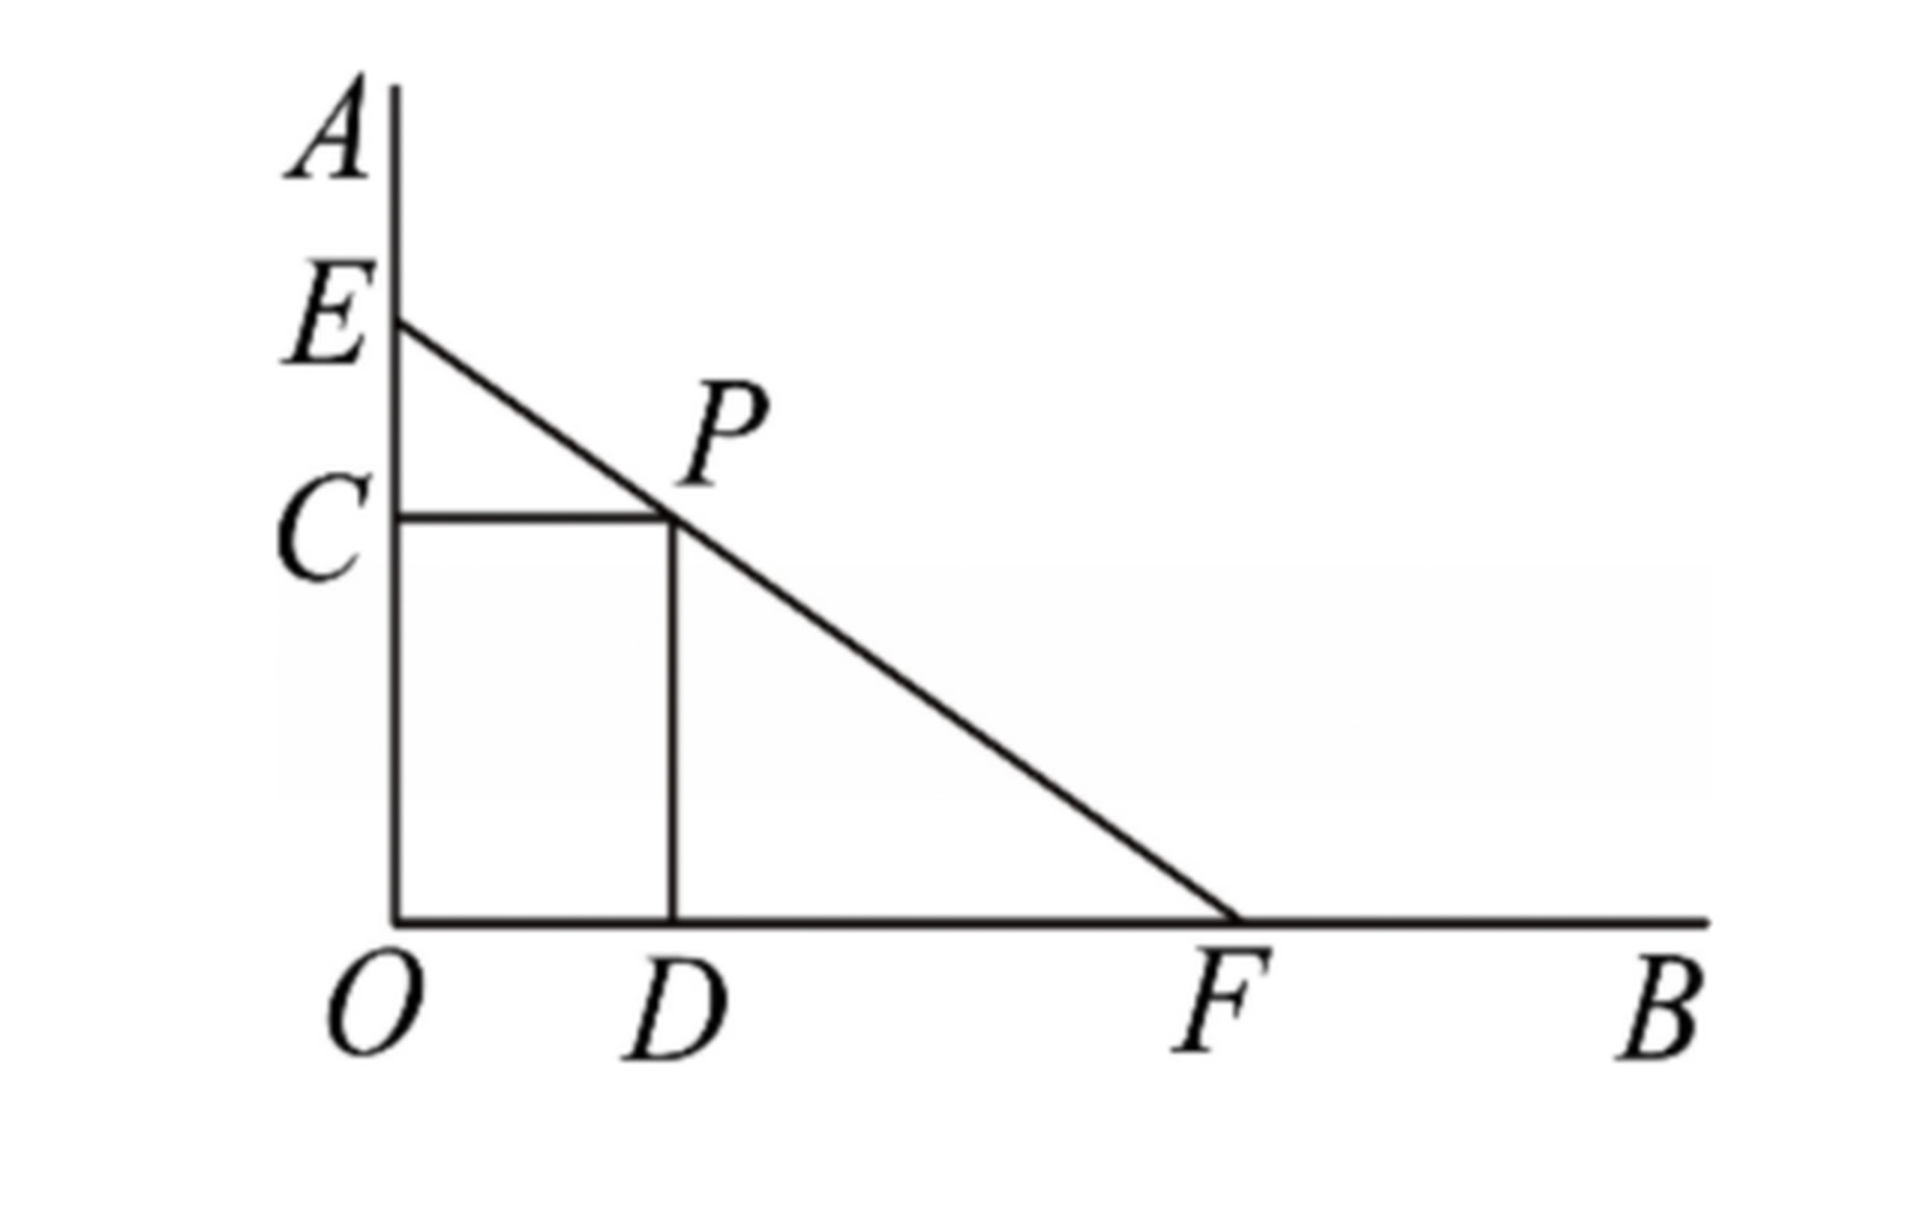
\includegraphics[width=0.32\textwidth]{figures/gao132_q18.png}
\end{center}

\ifanswer
\solbegin
\step{(1) 由题意得 $x\leq60$，}
\step{$\triangle PCE\sim\triangle FDP$，所以 $\dfrac{EC}{CP}=\dfrac{PD}{DF}$，即 $\dfrac{x}{25}=\dfrac{40}{DF}$，得 $DF=\dfrac{1000}{x}$m，}
\step{所以 $OF=OD+DF=\left(25+\dfrac{1000}x\right)$m，}
\step{所以 $25+\dfrac{1000}x\leq100$，解得 $x\geq\dfrac{40}3$；}
\step{综上，$\dfrac{40}3\leq x\leq60$；}
\step{(2) 由 $OE=OC+CE=(40+x)$m，}
\step{所以 $S=\dfrac12 OF\cdot OE=\dfrac12\left(25+\dfrac{1000}x\right)(40+x)$}
\step{$=\dfrac12\left(1000+25x+\dfrac{40000}x+1000\right)$m$^2$，}
\step{由基本不等式得 $S\geq\dfrac12\left(2000+2\sqrt{25x\cdot\dfrac{40000}x}\right)=2000$m$^2$，}
\step{当且仅当 $25x=\dfrac{40000}x$，即 $x=40$ 时取等号，}
\step{故 $EC=40$m 时，$S$ 取得最小值，为 $2000$m$^2$.}
\solend
\fi

\item 已知 $a>0$，$b>0$，请选择适当的方法证明.

(1) 若 $a\ne b$，证明：$a^3+b^3>a^2b+ab^2$；

(2) 若 $ab=1$，证明：$a^2+a<2$ 与 $b^2+b<2$ 不能同时成立.

\ifanswer
\solbegin
\step{(1) 因为 $a>0$，$b>0$，$a\ne b$，}
\step{所以 $a^3+b^3-a^2b-ab^2=a^2(a-b)+b^2(b-a)$}
\step{$=(a^2-b^2)(a-b)=(a-b)^2(a+b)>0$，所以 $a^3+b^3>a^2b+ab^2$.}
\step{(2) 假设 $a^2+a<2$ 与 $b^2+b<2$ 同时成立，所以 $-2<a<1,-2<b<1$，}
\step{又因为 $a>0,b>0$，所以 $0<a<1,0<b<1$，}
\step{所以 $0<ab<1$，这与 $ab=1$ 矛盾，}
\step{故 $a^2+a<2$ 与 $b^2+b<2$ 不可能同时成立.}
\solend
\fi

\item 若设 $M(a,n)=\lvert ax-1\rvert+\lvert ax-2\rvert+\cdots+\lvert ax-n\rvert$ 为曼哈顿扩张距离，它由 $n$ 个绝对值之和组成，其中 $n$ 为正整数.

(1) 若 $M(2,1)\leq5$，求 $x$ 的取值范围；

(2) 若 $k\leq M(2,2)$ 对一切实数 $x$ 恒成立，求实数 $k$ 的取值范围；

(3) $M(2,6)$ 是否存在最小值？若存在，求出该最小值与此时实数 $x$ 的取值范围；若不存在，说明理由.

\ifanswer
\solbegin
\step{(1) $M(2,1)=\lvert2x-1\rvert\leq5$，则不等式可化为 $-5\leq2x-1\leq5$，解得 $-2\leq x\leq3$，}
\step{所以 $x$ 的取值范围为 $[-2,3]$.}
\step{(2) 因为 $k\leq M(2,2)=\lvert2x-1\rvert+\lvert2x-2\rvert$ 对一切实数 $x$ 恒成立，}
\step{又 $\lvert2x-1\rvert+\lvert2x-2\rvert\geq\lvert(2x-1)-(2x-2)\rvert=1$，}
\step{当且仅当 $(2x-1)(2x-2)\leq0$，即 $\dfrac12\leq x\leq1$ 时取等号，}
\step{故 $k\leq1$，所以实数 $k$ 的取值范围为 $(-\infty,1]$.}
\step{(3) $M(2,6)=\lvert2x-1\rvert+\lvert2x-2\rvert+\lvert2x-3\rvert+\lvert2x-4\rvert+\lvert2x-5\rvert+\lvert2x-6\rvert$}
\step{$=2\left(\left\lvert x-\dfrac12\right\rvert+\lvert x-1\rvert+\left\lvert x-\dfrac32\right\rvert+\lvert x-2\rvert+\left\lvert x-\dfrac52\right\rvert+\lvert x-3\rvert\right)$，}
\step{其中 $\left\lvert x-\dfrac12\right\rvert+\lvert x-1\rvert+\left\lvert x-\dfrac32\right\rvert+\lvert x-2\rvert+\left\lvert x-\dfrac52\right\rvert+\lvert x-3\rvert$ 的几何意义为}
\step{在数轴上一点 $x$ 到 $\dfrac12,1,\dfrac32,2,\dfrac52,3$ 的距离之和，}
\step{要想距离之和最小，其中 $x\in\left[\dfrac12,3\right]$ 时，$\left\lvert x-\dfrac12\right\rvert+\lvert x-3\rvert$ 取得最小值，}
\step{当 $x\in\left[1,\dfrac52\right]$ 时，$\lvert x-1\rvert+\left\lvert x-\dfrac52\right\rvert$ 取得最小值，}
\step{当 $x\in\left[\dfrac32,2\right]$ 时，$\left\lvert x-\dfrac32\right\rvert+\lvert x-2\rvert$ 取得最小值，}
\step{综上，当 $x\in\left[\dfrac32,2\right]$ 时，$\left\lvert x-\dfrac12\right\rvert+\lvert x-1\rvert+\left\lvert x-\dfrac32\right\rvert+\lvert x-2\rvert+\left\lvert x-\dfrac52\right\rvert+\lvert x-3\rvert$}
\step{取得最小值，最小值为 $3-\dfrac12+\dfrac52-1+2-\dfrac32=\dfrac92$，}
\step{故 $M(2,6)=2\left(\left\lvert x-\dfrac12\right\rvert+\lvert x-1\rvert+\left\lvert x-\dfrac32\right\rvert+\lvert x-2\rvert+\left\lvert x-\dfrac52\right\rvert+\lvert x-3\rvert\right)$ 的}
\step{最小值为 $9$.}
\solend
\fi

\item 已知集合 $A=\{a_1,a_2,\cdots,a_n\}(0\leq a_1<a_2<\cdots<a_n,n\in\N,n\geq3)$ 具有性质 $Q$：对任意 $i,j(1\leq i\leq j\leq n)$，$a_i+a_j$ 与 $a_j-a_i$ 至少有一个属于集合 $A$；

(1) 判断集合 $M=\{0,2,4\}$ 与 $N=\{2,3,4\}$ 是否具有性质 $Q$，并说明理由；

(2) 已知 $A=\{a_1,a_2,a_3\}$ 具有性质 $Q$，当 $a_2=2026$ 时，求集合 $A$；

(3) 已知 $B=\{b_1,b_2,\cdots,b_{2026}\}$ 具有性质 $Q$，求 $\dfrac{b_1+b_2+\cdots+b_{2026}}{b_{2026}}$ 的值；

\ifanswer
\solbegin
\step{(1) 集合 $M=\{0,2,4\}$ 中，}
\step{因为 $0+2\in M,0+4\in M,4-2\in M,0\pm0=0\in M$，}
\step{$2+2=4\in M,2-2=0\in M,4-4=0\in M$，所以集合 $M$ 具有性质 $Q$；}
\step{集合 $N=\{2,3,4\}$ 中，因为 $3+3=6\notin N,3-3=0\notin N$，}
\step{所以集合 $N$ 不具有性质 $Q$.}
\step{(2) 因为 $a_1<a_2<a_3$，且 $A=\{a_1,a_2,a_3\}$ 具有性质 $Q$，}
\step{所以 $a_3+a_3\notin A,a_3-a_3=0\in A$，则 $a_1=0$，}
\step{又因为 $a_2+a_3>a_3$，所以 $a_2+a_3\notin A$，则 $a_3-a_2\in A$，}
\step{由集合的互异性得 $a_3-a_2=a_2$，而 $a_2=2026$，所以 $a_3=4052$，}
\step{故 $A=\{0,2026,4052\}$；}
\step{(3) 先证明一般结论：$A=\{a_1,a_2,\cdots,a_n\}(0\leq a_1<a_2<\cdots<a_n,n\in\N,n\geq3)$}
\step{具有性质 $Q$，则 $a_1+a_2+a_3+\cdots+a_n=\dfrac n2 a_n$.}
\step{因为 $A=\{a_1,a_2,\cdots,a_n\}(0\leq a_1<a_2<\cdots<a_n,n\in\N,n\geq3)$ 具有性质 $Q$，}
\step{所以 $a_n+a_n\notin A$，则 $a_n-a_n=0\in A$，则 $a_1=0$.}
\step{又因为 $0\leq a_1<a_2<\cdots<a_n$，所以 $0\leq a_n-a_n<a_n-a_{n-1}<\cdots<a_n-a_1$，}
\step{又因为 $a_n+a_{n-i}>a_n(i=1,2,\cdots,n-1)$，所以 $a_n+a_{n-i}\notin A$，}
\step{则 $a_n-a_{n-i}\in A$，}
\step{所以 $a_1=a_n-a_n,a_2=a_n-a_{n-1},a_3=a_n-a_{n-2},\cdots,a_n=a_n-a_1$.}
\step{所以 $a_1+a_2+a_3+\cdots+a_n$}
\step{$=(a_n-a_n)+(a_n-a_{n-1})+(a_n-a_{n-2})+\cdots+(a_n-a_1)$，}
\step{即 $a_1+a_2+a_3+\cdots+a_n=\dfrac n2 a_n$，}
\step{所以 $B=\{b_1,b_2,\cdots,b_{2026}\}$ 具有性质 $Q$，则 $b_1+b_2+\cdots+b_{2026}=\dfrac{2026}{2}b_{2026}$，}
\step{所以 $\dfrac{b_1+b_2+\cdots+b_{2026}}{b_{2026}}=\dfrac{2026}{2}=1013$.}
\solend
\fi

\end{enumerate}

% 行数复核：逐题数 \step 条数，合计 144 条（Q3：4；Q4：1；Q5：4；Q6：2；Q7：9；Q8：2；
% Q9：3；Q10：6；Q11：9；Q12：9；Q13：0；Q14：9；Q15：4；Q16：19；Q17：5；Q18：11；
% Q19：7；Q20：17；Q21：23），与原卷印刷行逐题相等（cases 块作一个印刷行计）。
% 第 13 题只印括号内答案、提 \ans{}，不计入 \step 账；第 14—16 题答案在解析末句，
% 括号内留空、不另提 \ans{}。

\end{document}
